% !TEX TS-program = pdflatex
% !TEX encoding = UTF-8 Unicode

% Example of the Memoir class, an alternative to the default LaTeX classes such as article and book, with many added features built into the class itself.

\documentclass[12pt,a4paper]{memoir} % for a long document
%\documentclass[12pt,a4paper,article]{memoir} % for a short document
\newif\iftth
\iftth\else
\usepackage{makeidx}
\makeindex
\usepackage[utf8]{inputenc} % set input encoding to utf8
\usepackage{moreverb}
\usepackage{graphicx}
\usepackage{longtable}
\usepackage{pifont}
\usepackage{color}
../texdoc/rgb.tex
\usepackage[table]{xcolor}
\usepackage{fancyvrb}
\fi
\usepackage{bbding}
\definecolor{lightblue}{rgb}{0,0,1}
\definecolor{lightred}{rgb}{1,0,0}
\iftth\else
\usepackage{tikz}
\usetikzlibrary{mindmap,trees,snakes}
\fi
%\definecolor{tableShade}{HTML}{F1F5FA}   %iTunes
%\definecolor{tableShade2}{HTML}{ECF3FE} %Finder

%\usepackage{lscape}
\usepackage{pdflscape}
%\usepackage{listings}
%\usepackage{tikz}
%\usepackage{utopia}
%\usepackage[explicit]{titlesec}

%\lstset{language=C,basicstyle=\ttfamily,numbers=left,numberstyle=\tiny}
% Don't forget to read the Memoir manual: memman.pdf

%%% Examples of Memoir customization
%%% enable, disable or adjust these as desired

%%% PAGE DIMENSIONS
% Set up the paper to be as close as possible to both A4 & letter:
%\settrimmedsize{297mm}{210mm}{*} % letter = 11in tall; a4 = 210mm wide
%\setlength{\trimtop}{0pt}
%\setlength{\trimedge}{\stockwidth}
%\addtolength{\trimedge}{-\paperwidth}
%\settypeblocksize{*}{\lxvchars}{1.618} % we want to the text block to have golden proportionals
%\setulmargins{50pt}{*}{*} % 50pt upper margins
%\setlrmargins{*}{*}{1.618} % golden ratio again for left/right margins
%\setheaderspaces{*}{*}{1.618}
%\setheadfoot{\onelineskip}{2\onelineskip}
%\checkandfixthelayout 

%\title{\textsl{A container library for C}}

%\settrimmedsize{297mm}{210mm}{*}
%\setlength{\trimtop}{0pt}
%\setlength{\trimedge}{\stockwidth}
%\addtolength{\trimedge}{-\paperwidth}
\iftth\else
\settypeblocksize{634pt}{448.13pt}{*}
\setulmargins{4cm}{*}{*}
\setlrmargins{30mm}{*}{*}
\setmarginnotes{17pt}{51pt}{\onelineskip}
\setheadfoot{\onelineskip}{2\onelineskip}
\setheaderspaces{*}{2\onelineskip}{*}

\checkandfixthelayout
\fi
\newenvironment{ShorterItemize}{
\begin{itemize}
\iftth\else
  \setlength{\itemsep}{1pt}
  \setlength{\parskip}{0pt}
  \setlength{\parsep}{0pt}
\fi
}{\end{itemize}
}

\iftth\else
%%% ToC (table of contents) APPEARANCE
\maxtocdepth{subsection} % include subsections
\fi
\renewcommand{\cftchapterpagefont}{}
\renewcommand{\cftchapterfont}{}     % no bold!

%%% HEADERS & FOOTERS
\iftth\else
\pagestyle{ruled} % try also: empty , plain , headings , ruled , Ruled , companion

%%% CHAPTERS
\chapterstyle{hangnum} % try also: default , section , hangnum , companion , article, demo
\fi
\renewcommand{\chaptitlefont}{\Huge\sffamily\raggedright} % set sans serif chapter title font
\renewcommand{\chapnumfont}{\Huge\sffamily\raggedright} % set sans serif chapter number font

\iftth\else
%%% SECTIONS
\hangsecnum % hang the section numbers into the margin to match \chapterstyle{hangnum}
\maxsecnumdepth{subsection} % number subsections

\setsecheadstyle{\Large\sffamily\raggedright} % set sans serif section font
\setsubsecheadstyle{\large\sffamily\raggedright} % set sans serif subsection font
\fi
%% END Memoir customization
\newcommand{\raisedrule}[2][0em]{\leaders\hbox{\rule[#1]{1pt}{#2}}\hfill}

\title{\textsl{A container library for C}}
\author{Jacob Navia}
\date{} % Delete this line to display the current date
\usepackage{xargs}
\usepackage{color}
%\renewcommandx*{\hrulefill}[2][0pt]{\leavevmode \leaders \hbox to 1pt{\rule[#1]{1pt}{#2}} \hfill \kern 0pt}
\iftth\else
\renewcommandx*{\hrulefill}[2][1=0.3mm,2=0pt]{\leavevmode \leaders \hbox to 1pt{\rule[#2]{1pt}{#1}} \hfill \kern 0pt}
\fi
\definecolor{purple}{rgb}{0.42,0.12,1.0}

%--------------------------------------------------API
\newcommand{\api}[1] {%
 \iftth\else\Needspace{3\baselineskip}\fi%
\par\vspace{0.4cm}
\addcontentsline{toc}{subsubsection}{#1}
\index{#1!\container}
\addtocounter{apis}{1}
%\par\noindent
\noindent {\large \textbf{#1}} \hrulefill%[1pt][3.5pt]
\iftth\else
\nopagebreak
\fi
\begin{verbatim}
}

\newcommand{\container}{}
%% --------------------------------------- Function command
\newcommand{\function}[1] {%
\vspace{0.2in}
\par\noindent
\textbf{#1}\index{#1!code for \container} \hrulefill
\iftth\else
\nopagebreak
\fi
\noindent\begin{Verbatim}[numbers=left, xleftmargin=7mm]}



%% Description command
\newcommand{\apidescription}{%
\par \noindent \textbf{Description:} %\par\noindent
}
\newcommand{\notes}{
\par \noindent \textbf{Notes:}\par\noindent}

\newcommand{\apierrors}{%
\par \noindent \textbf{Errors:}\par\noindent
}
\newcommand{\doerror}[1]{%
\par\noindent
\iftth
{CONTAINER\_ERROR\_#1}
\else
{\footnotesize CONTAINER\_ERROR\_#1}
\fi
}
\newcommand{\notfound}{
{\footnotesize CONTAINER\_\-ERROR\_\-NOTFOUND}
}

\newcommand{\Const}{
{\par\noindent \textbf{Invariants:}\noindent}
}

\newcommand{\Null}{{\iftth \ NULL \else \footnotesize NULL\  \fi}}

\newcommand{\Type}{{\iftth \ DATA\_TYPE \else \footnotesize DATA\_TYPE\  \fi}}


\newcommand{\X}{
%\colorbox{blue!30}
%{\normalsize \textbf{$\oplus$}}
{\ding{53}}
}

\newcommand{\returns}{\par\noindent\textbf{Returns:}}
\newcommand{\example}{
\par\noindent
\textbf{Example:}
\begin{verbatim}
}
\newcommand{\param}[1]{
\texttt{\textsl{#1}}
}
\newcommand{\See}[1]{%
see \S\ref{#1} on page~\pageref{#1}
}
\iftth\else
%______________________________________________
\newcommand*{\titleJT}{\begingroup% Jan Tschichold: typographer 
%\FSfont{5gm} % FontSite Garamond 
\drop = 0.08\textheight \vspace*{\drop}
\hspace*{0.3\textwidth} {}\\[1\drop] 
\hspace*{0.3\textwidth}
{\Huge\itshape\raggedleft A container library for C}\par \vspace{13cm} {\raggedleft\Huge\itshape Jacob Navia\  \par} \vfill \hspace*{0.3\textwidth}{\Large \raggedleft }\\[0.5\baselineskip] \hspace*{0.3\textwidth}{\Large } \vspace*{\drop} \endgroup}
\newlength{\drop}
\fi
\makeindex
\newcounter{apis}
%______________________________________________
%%% BEGIN DOCUMENT
\begin{document}
\iftth\else
\VerbatimFootnotes
\setcounter{tocdepth}{5}
\fi
\setcounter{apis}{0}
\iftth\else\pagestyle{empty} \titleJT\fi
%\cleardoublepage
%\maketitle

\pagestyle{empty}
\newpage
\hspace*{-1.0in}
%\addtolength{\topmargin}{-1.8in}
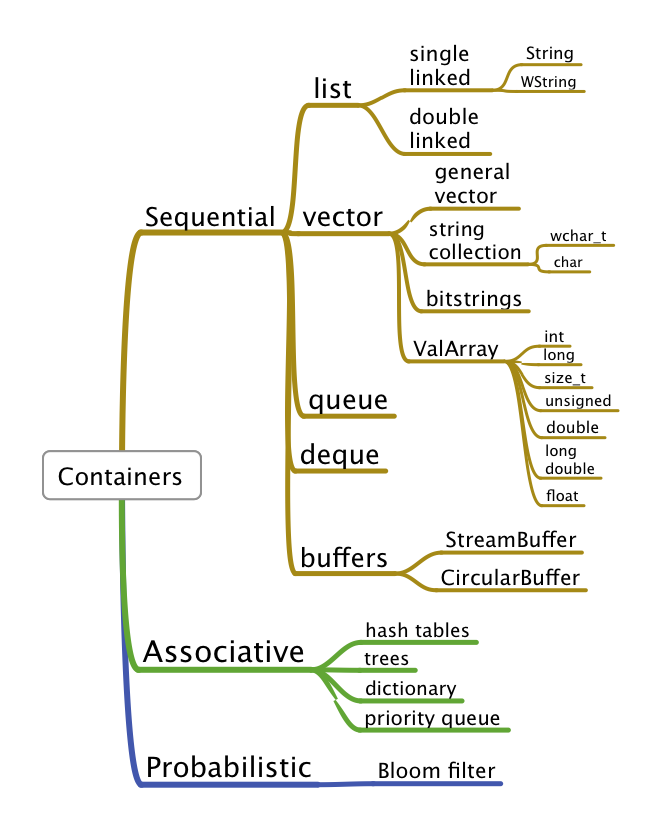
\includegraphics[scale=0.65]{Containers.png}
\cleardoublepage
%\addtolength{\topmargin}{1.8in}
\pagestyle{headings}

\tableofcontents* % the asterisk means that the contents itself isn't put into the ToC
\iftth\else\pagestyle{headings}\fi
\chapter{Introduction}
%--------------------------------------------------------------------------------------------------------------------------
%                                                   INTRODUCTION
%--------------------------------------------------------------------------------------------------------------------------
The objective of this proposal is to standardize the usage of common data structures within the context of the C language. The existence of a common standard interface for lists, hash tables, flexible arrays, and other containers has several advantages:
\begin{itemize}
\item
User code remains portable across different projects. In C, we all use the FILE abstraction, for instance. This abstraction allows software to be 
compatible across a large spectrum of machines and operating systems. Imagine what would happen if each project had to develop a file stream
abstraction again and again. This is the case when using lists, for instance. Today, we have in all significant projects written in C a list
module, and probably other ones like hash tables, etc. 

\item Avoid duplication of effort. Most of the list or hash tables modules can't be debugged completely and are the source of never ending problems.
\item Lack of standards makes the merging of two projects very difficult since in most cases the interfaces and data structures are slightly
different. This leads to a complete rewrite of one of the modules, or to "adapter" software that will translate from one list implementation
to the other, adding yet another layer of complexity to the merged project.
\item The language becomes more expressive since it becomes possible to reason within a high level environment. The lack of operations for
handling advanced data structures conditions programmers to use low level solutions like making an array with a fixed maximum size instead of a
list even if the programmer would agree that a list would be a more adequate solution to the problem. Confronted to the alternative of
developing yet another list module or opting for a low level solution many time constrained programmers will opt for the second solution.
\item
The portable specifications provide a common framework for library writers and compiler/system designers to build compatible yet strongly specialized implementations.
\item
The language becomes easier to analyze mathematically.
In their very interesting paper "Precise reasoning for programs using containers", Dillig, Dillig and Aiken
\footnote{"Precise Reasoning for programs using containers" Isil Dillig, Thomas Dillig, and Alex Aitken, available on line at
http://www.stanford.edu/\string~isil/popl2011.pdf or at POPL 2011 Proceedings of the 38th annual ACM SIGPLAN-SIGACT symposium on Principles of programming languages
ACM New York, NY, USA ©2011 } enumerate three main points that make program analysis easier using containers:
\begin{enumerate}
\item Understanding the contents of a container doesn't require understanding the container's implementation
\item Verifying container implementations requires different techniques and degrees of automation than verifying their clients. Hence, separating
these two tasks allows us to choose the verification techniques best suited for each purpose.
\item There are orders of magnitude more clients of a container than there are container implementations. This fact makes it possible to annotate
a handful of library interfaces in order to analyze many programs using these containers.
\end{enumerate}
\item It is possible to abstract from the nature of any container (using the \texttt{iterator} construct) what allows a series of algorithms to
be written without having to bind them to a precise data structure. Containers present a uniform interface to the rest of the program.
\end{itemize}
\par
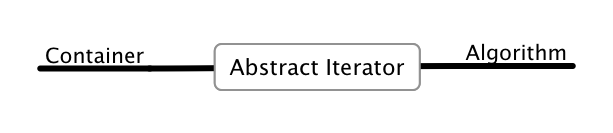
\includegraphics[scale=0.63]{AbstractIterator.png}
\par
The big innovation of C in the eighties was its standard library, that made input/output portable across machines and implementations. The container library would replicate again that idea, at a higher level.

The specifications presented here are completely scoped by the C99 specifications, and can be implemented even in compilers that do not implement C99 and remained within the C94 context. No language extensions are needed nor any are proposed.


The interfaces proposed try to present complete packages, i.e. interfaces with all the necessary functions to allow the widest usage: Serialization, searching, and many other functionalities are included in the proposed standard to allow for maximum code portability. It can be argued that this makes  for "fat" containers, but if you read carefully you will notice that many things can be left out in systems that run in low memory or with feeble computing power.

This documentation is composed of several parts:
\begin{enumerate}
\item An introductory part where the general lines of the library are explained.
\item A specifications part where each function of the library is fully specified. This is the proposal for the next C standard.
\item An "examples" part that shows the uses of the library and allows you to have a better idea of how the usage of the library looks like.
\item An implementation part where the code of the sample implementation is discussed. This is designed as a guide for implementors to give them a basis to start with.
\end{enumerate}
%
%---------------------------------------------------------------------------Design Goals
%
\section{Design goals}
\subsection{Error analysis}
It has been a  tradition in C to place raw performance as the most important quality of specifications. To follow this sacred cow, C specifications
ignored any error analysis arguing that any specification of failure modes would damage "performance". No matter that raw machine performance
increased by several orders of magnitude, the cost of  a check for NULL was always "too expensive" to afford.

This kind of mental framework was described by one of the people in the discussion group "comp.lang.c++" as follows:\footnote{We were discussing 
the specifications of the \texttt{mismatach} function of the C++ STL and why any error analysis is absent. The C++ STL prescribes a bounded 
region for the first container, but just a starting point for the second one. If the second is shorter than the specified range of the first
 \textsl{undefined behavior} ensues and anything can happen. In many cases this "anything" is different each time the same error occurs. In our
specific case \texttt{mismatch} would read from memory that doesn't belong to the container it started with. Depending on the contents of
that memory a crash could happen, or worst, a wrong result returned to the calling software, etc.}
\begin{quotation}
 In C++, the program is responsible for ensuring that \textbf{all} parameters to
 the standard library functions are valid, not only the third parameter of
 \texttt{std::mismatch()}. For example, also the first range for \texttt{std:mismatch()}
 must be valid, one may not pass a start iterator from one container and
 end iterator from another, for example. However, STL does not guarantee
 any protection against such errors, this is just UB.
\end{quotation}
These specifications try to break away from that frame of thought. Each function specifies a minimal subset of failure modes as a consequence of its 
error analysis. This allows user code to:
\begin{itemize}
\item Detect and handle errors better. Error detection is simple: Almost all functions return a negative
error code when they detect an error condition. Error detection can always test for the result
of any API with:
\begin{verbatim}
if (SomeCclApi(arg1,arg2) < 0) {
    // error handling here
}
\end{verbatim}

Some functions like the \verb,Create, function return a pointer. In those cases an error provokes a NULL 
pointer result. The error checking in those cases should be:
\begin{verbatim}
if ((r=SomeCclApi(arg1,arg2)) == NULL) {
    // error handling here
}
\end{verbatim}
\item Ensure that errors will always have the \textbf{same} consequences. One of the worst consequences of undefined behavior is that the same error can 
have completely different consequences depending on apparently random factors like previous contents of memory or previous allocation pattern.
\end{itemize}

At the same time, the mandatory error checking consists mainly of checks that can be implemented with a few integer comparisons. For instance a check 
for zero is a single instruction in most processors. If implemented correctly the conditional jump after the comparison with zero is not taken in the 
normal case and correctly predicted by the processor. This means that the pipeline is not disturbed and the cost for the whole operation is much less than a cycle.

Why is error analysis an essential part of any program specifications?

Because \textbf{mistakes are a fact of life}. Good programmers are good most of the time only. Even very good programmers \textsl{do make mistakes\footnote{Donald Knuth, the author of the TeX typesetting program can be without doubt be qualified as a good programmer (and an excellent computer scientist). But he, like anybody else, is not without flaws. See: 
www.tug.org/texmf-dist/doc/generic/knuth/errata/errorlog.pdf. There are hundreds of entries in that log.}.} Software
must be prepared to cope with this fact in an orderly fashion because if failure modes are not specified they have catastrophic consequences and lead
to brittle software that crashes randomly.

Note that error \textsl{analysis} is not error \textsl{handling}. Error handling is taking an action after an error, a task only the application can do.
What the library can do is to establish a framework where a user defined procedure receives enough information about the specific problem at hand.

Error analysis means that for each function and each API:
\begin{itemize}
\item An analysis is performed of what are the consequences of any error in its inputs. Error codes are used to pass detailed error information
to the error procedure.
\item During its execution, an analysis is done of each step that can fail.
\item The outputs of the function are left in a consistent state, errors provoking the undo of the previous steps in most cases, leaving the inputs
as they were before the function was called. This feature allows library functions to be restartable after an error. For instance an out of memory
condition can be corrected by freeing memory and retrying.
\end{itemize}
The library provides hooks for the users that can control each step and provide functions that can do the error handling, for instance logging the
error and jumping to a pre-established recovery point.
\subsection{Full feature set}
Another design goal is to offer to the user a full feature set, complete with serializing, iterators, search, read-only containers and all the features 
needed in most
situations. Other features are planned for later like multi-threading support. The objective here is to avoid incompatible and non portable extensions
because some essential feature is missing.
\subsection{Abstraction}
The library is designed with the possibility of implementing abstraction like serial and associative containers that allow software to treat several 
containers in a way that abstract most of their features, improving code reuse by allowing to implement algorithms for a class of objects. This is
specially true in the iterators feature.

It can be argued that the C language lacks many of the abstractions constructs of other languages like templates, inheritance, and many others.
All that is true, but the objective of this proposal is to show that those constructs are just an aid to developing abstractions, an aid that
is paid in added complexity for the resulting language, and in a limitation of what is feasible within a given framework. Since C has no 
framework, no preferred inheritance model, it is possible to create abstractions that are quite unconstrained: there is no framework precisely.
\subsection{Performance} Even with all the tests, the performance of the library has been maintained at a high level compared to similar libraries
in other languages. The performance should improve if standardized because compiler writers could specialize their optimizations targeting this
code.
\subsection{Compile time checking}
The base implementation of the library uses \verb,void *, everywhere since the library can't know what type
of data the user is storing in it. This means that no compile-time checking can be done on the type of
arguments passed to a library function, what is very error prone.

To mitigate this problem the library offers a "templated" version of each container, where the user must
write a very small parameter file for a templated version that specifies a container for a specific data
type, allowing for compile time checking of arguments and a simpler syntax.

Note that no new language features are needed for this to work since it uses the preprocessor to specialize
a file template of the desired container. Most of the containers are provided in these two forms: a generic
version using void pointers and a templated version that builds a software layer between the generic version and
the specialized version allowing for compile time checking.

To speed up this process specialized versions of the list and vector containers are provided for most of the
basic types of the language: int, doubles, etc.
%-----------------------------------------------------------------------------------------------------------
%                                                       Typographical conventions
%-----------------------------------------------------------------------------------------------------------
\section{How the functions are specified in this document.}
The specifications part of the proposal uses the same building blocks for each of the functions proposed.\par\noindent
\textbf{Name}

\noindent The name of the function. Note that when using this name, the name of the container interface should be always before 
since this name is a field of the interface structure:

\noindent \verb,iList.Add,, \verb,iDictionary.Add,, etc.

\noindent The name is followed by the prototype defined as a function pointer. For the function \verb,Add, of the container \verb,List, we have
\begin{verbatim}
    int (*Add)(List *list,const void *data);
    int (*Add)(TYPEList *list,const TYPE data);
\end{verbatim} 
This means that \verb,Add, is a function pointer in the interface \verb,iList,. It would be used as:
\texttt{iList.Add(list,data)}.
The second line corresponds to the \textsl{template} form of the API. This is explained further down (\S \ref{TwoTypes} page-\pageref{TwoTypes}) and
it is specified only when the signature of the API diverges from the generic one. The \verb,TYPE, marker means that
a type name should appear there: in the example it could be intList, doubleList, CustomerList, etc.

\apidescription The API is described: purpose, inputs and outputs. Note that unmodified arguments are always marked
as \verb,const,.

\apierrors
The minimal set of errors that can appear during the execution of the function is listed. Each implementation 
is free to add implementation specific errors to this list. Note that how the library behaves after an error is 
defined by the current error function in the container (if any), then by the behavior of the error function in the 
\verb,iError, interface.

\returns
The return value of the operation. Normally, negative values are error codes, positive values means success, and zero means non fatal errors, more in the sense of a warning.

\section{Which sections of this document are normative?}
This document presents the C container Library to the C standardization committee. The following sections are normative:
\begin{itemize}
\item Chapter 4: The auxiliary interfaces. The required interfaces are:
\begin{ShorterItemize}
\item The mask interface
\item The memory management interface
\item The error handling interface
\item The iterator interface
\item The observer interface
\end{ShorterItemize}

The heap and pool interfaces are optional.
\item Chapter 5: The containers:
\begin{center}
\begin{longtable}{|p{3cm}|p{3cm}|p{2.5cm}|}
\hline
\textbf{Container}&\textbf{Interface}&\textbf{Required?}\\\hline
BitString&iBitString& \Checkmark \\
BloomFilter&iBloomFilter&\XSolidBrush \\
CircularBuffer&iCircularBuffer& \Checkmark \\
Deque&iDeque&\Checkmark \\
Dictionary&iDictionary&\Checkmark \\
Dlist&iDlist&\Checkmark \\
HashTable&iHashTable&\XSolidBrush \\
List&iList&\Checkmark \\
Queue&iQueue&\Checkmark \\
PQueue&iPriorityQueue&\Checkmark \\
StreamBuffer&iStreamBuffer&\Checkmark \\
StringList&iStringList&\Checkmark\\
strCollection&istrCollection&\Checkmark \\
TreeMap&iTreeMap&\Checkmark \\
Value array&iValArrayXXX&\Checkmark \\
Vector&iVector&\Checkmark \\
WstrCollection&iWstrCollection&\XSolidBrush\\
\hline

\end{longtable}
\end{center}
The different ValArray containers should
include several basic data types like int, char or long.
Floating point types float and double are required, but not the types long long, long double and all complex types.
The rationale is to avoid excluding C implementations designed for very small processors or environments.
\end{itemize}
All text in footnotes, tables or drawings is not normative.

The order of the APIs within each interface is implementation defined. In general no assumptions should 
exist about any specific layout of the interfaces or data structures in the library. In the documentation
the APIs are listed following the alphabetical order.

\section{Practical tips}
The code of the sample implementation can be obtaned from:

\noindent\verb,http://code.google.com/p/ccl/,

Go to Downloads and there you will find the documentation (this document) and the source code in the form of a \verb,ccl.zip, file.
\index{Download!source} See also the chapter about the sample implementation in this document.


\chapter{Overview}
\section{Containers}
In the context of this library, a container is a data structure used to organize data within a single logical object that allows for adding, searching 
and removing data. In most containers the data is not further specified, but the library assumes that all elements of a container have the same type. 
The data can be anything, images, numbers, text, whatever. The only thing that the container knows is the size of the data, if we store a series of 
objects of the same size, or its address, if we store objects of different sizes. In the later case we store just a pointer in the 
container\footnote{Matthew Wilson uses a more restrictive definition of a container in his book "Extended STL (Vol 1, page 16)" :\par A container is a 
collection that owns its objects and provides operations by which those objects may be accessed and modified and, optionally, added removed and 
rearranged.\par By this definition, containers that have just pointers to their elements wouldn't be containers at all.}.

A special kind of containers, ValArrays, contain the basic types of the C language and the library treats them specially. There is one ValArray
for each elementary type. For character strings they are stored in "string collections", a term borrowed from the C\# language.

Each container has a way of iterating through all its elements by using an "iterator" auxiliary object, that returns each stored object in sequence. In 
sequential containers you can also iterate using an index variable, what can be cheaper than using iterators for arrays but very expensive in lists.

All objects stored by the library are copied into the library, and the library is responsible for the management of the associated storage. If you do not want this, just store a pointer to the data and manage the data yourself.

A container has a set of functions for accessing the elements it stores, called its \textsl{interface}. This object is a collection of function
pointers that provide the functionality of the container.  The interfaces are stored in writable memory and the user can, at run time, change the
behavior of a class of containers by changing the function pointer. This operation is called "subclassing" in this document.

Subclassing allows the user to modify the behavior of a container, maybe adding some functionality, without having to write all the container from
scratch. The user of the library can:
\begin{itemize}
\item Use the stored pointer to the original function to call the original functionality, and add some functionality after that call.
\item Add some functionality and call the stored pointer afterwards.
\item Replace completely the functionality by its own without calling any of the former functions.
\end{itemize}
Subclassing adds enormous flexibility to this design, since it makes possible to add functionality in a transparent way.

Using the organization of the data as a classification criteria we have basically two different kinds of containers
\begin{itemize}
\item
1. Sequential containers
\item
2. Associative containers
\item
3. Statistical Containers
\end{itemize}

A sequential container is organized in a linear order. We have a sequence starting at index zero up to the number of elements stored. Data items can be 
retrieved by index, and it makes sense to speak of a "next" and a "previous" element.

Sequential containers can be contiguous (arrays) or disjoint (lists). In the first case access is very fast since it implies multiplying the index by 
the size of each element to get to any position in the data. In the second case access the nth element can be a lengthy operation since the chain of 
"next" or "previous" pointers must be followed for each access to a given position.

An associative container stores an object divided in two parts: a key, that is used as a token for the data, and the data itself. It associates 
key/value pairs. Speed of access is fast, but not linear, and can degrade as new items are stored in it.

Statistical containers are containers that return the probability of an item being found in them. See the bloom filter as an example.

In all cases, we have some basic properties of an abstract container that are common to all of them. 
\begin{itemize}
\item Functions to implement the life-cycle of the object: creation, maintenance and destruction.
\item Functions to add, replace and remove elements from the container.
\item A function that returns the number of objects stored in the container.
\item
A function to report errors. This function (like all other function pointers) can be changed by the user of the library. In the sample implementation 
it defaults to a simple function that prints the error in the standard error stream. 
\item
Each change in a container is recorded. This permits to validate pointers to a container: if the container has changed after the creation of the pointer, the pointer could be invalid.
\item
All containers use a standard object to allocate and manage memory. The library provides a default allocator that contains the standard C functions malloc, free, realloc and calloc. Each container class can contain an allocator pointer, or each container can contain an allocator. The provided
sample implementation has a per container allocator, but in many applications a per class allocator could be enough, or even a single global allocator
that would be used by the whole library.
\end{itemize}

Managing a sequence involves trade offs what performance is concerned. If the usage will involve frequent insertion and deletion of objects you will 
prefer a container that handles those operations in constant time: the time to add or delete an object doesn't increase with the number of elements in 
the container. Such a container will be unlikely to provide also access to a given element in constant time. Access is likely to be much slower, and 
what you gain in flexibility you loose in another dimension. It is the user of the library, the programmer, that decides what container fits best the 
intended usage.

Since usage patterns change, however, the library tries to ensure that you can change the container you are using with minimal effort. If at the 
beginning of an application a list looked like a good solution but later an array, that provides constant time access is better suited, you can change 
the type of container without changing every line that uses it. The common vocabulary of the library makes this possible.

\section{The two types of interface}
\label{TwoTypes}
The library proposes two types of access:
\begin{itemize}
\item A generic approach using \verb,void *,. This interface allows you to pass a pointer to the data and specify at creation time the size of the 
object you want to store in the container. There is no checking at compile-time of the validity of the pointer and the associated data. There is no 
checking at run time either since the software has no information to check something.
\item A templated generic approach where at compile time a \textsl{templated} file is specialized for a concrete type by writing a parameter file
where some macros are defined that are used by the templated file as arguments. The user of the library is required to write that file, compile
it, and adding the resulting object files to a user-specific library (or to the general containers library if he/she wishes) so that the linker finds 
them when needed.

\end{itemize}
The functions to call, their names, etc, are the same in both approaches with one important exception: the templated approach needs an object instead 
of a \verb,void *, to the data as parameter, and returns an object instead of a void pointer to the data.

For instance, when writing for the generic interface you use:
\begin{verbatim}
double MyDouble;
List *myList;
myList = iList.Create(sizeof(double));
// ...
iList.Add(myList,&myDouble);
\end{verbatim}

For the templated interface you use:
\begin{verbatim}
double MyDouble;
doubleList *myList;
myList = idoubleList.Create();
// ...
idoubleList.Add(myList,myDouble);
\end{verbatim}


Naming rules allow the user of the templated library to easily add
the required names to its program and use them. The naming rules are explained further down.

The drawback of the second approach is a bigger complexity of the compilation process. When using a template container the user must:
\begin{itemize}
\item Give the parameters that the templated file needs. In most cases the minimum requirements are that the data type is specified:
\begin{verbatim}
#undef DATA_TYPE
#define DATA_TYPE Customer
#include "listgen.h"
\end{verbatim}

This will produce the definitions of the following types:
\begin{itemize}
\item The \verb,CustomerList, container and its \verb,iCustomerList, interface.
\item The \verb,iCustomerListIterator,: an iterator type ready to be used with any \verb,CustomerList, containers.
\end{itemize}
\item Include the type specific header. For instance \verb,#include "Customerlist.h",. All client code that uses the derived container must
include that header.
\item Compile the instantiation of the template:
\begin{verbatim}
#undef DATA_TYPE
#define DATA_TYPE Customer
#include "listgen.c"
\end{verbatim}

The resulting object file must be present at link time, either stand alone or within a library.
\end{itemize}

\section{The interface concept}
Each container is defined by its interface, i.e. the table of functions it supports. For each interface, its name is composed of a lower case "i" followed by the container name: \verb,iList,, \verb,iVector,, \verb,istrCollection,, etc.

Each function of the interface receives always the container as its first argument. Obviously, the big exception is the creation function, that receives various arguments depending of which container or from what input, the container is to be created.

For each container interface a global object exists that allows direct access to the function table without the need of creating a container to access it.

This interface allows for simple access to each container using a very similar vocabulary:
\begin{verbatim}
iList.Add(list,object);
istrCollection.Add(strcol,object);
\end{verbatim}
The objects stored in a container have always the same size. When storing objects of different sizes just store a pointer to the objects, since pointers have always the same size.
\section{Error handling}
This specification describes the basic error handling that each function of the library must do. Other errors can appear in different implementations.

Error handling has three different phases:
\begin{enumerate}
\item \textbf{Detection}. All library functions detect blatantly wrong arguments for instance, a \Null pointer when an object is expected, or arguments out of their valid range, etc.
\item \textbf{Reporting.} When an error is detected the library calls the corresponding error function that receives a character string with the name of the 
function where the error was detected, an integer error code, and possibly other arguments. Error codes are always negative constants.
\item \textbf{Response.} The library's default response to an error is to print it in the standard error stream. This can be modified by the user at any time by calling the \texttt{SetErrorFunction} API, replacing the default behavior with its own.

The response strategy can be changed at two levels \footnote
{Some implementations can do additional levels. For instance an implementation can add a container specific level by adding some error function
to the interface of the container that would be called before the global, library wide error function is called.}:
\begin{ShorterItemize}
\item At the individual container level, by changing the error function called in  most cases when an error occurs for this specific container. The
API \verb,SetErrorFunction, is specifically designed for this purpose.
\item At the container library level by changing the default error function in the \verb,iError, interface.
\end{ShorterItemize}

\end{enumerate}

At each error, the library calls the container instance specific error handling function. This function is initialized to the default error
function of the library when the container is created. When it is not possible to call the instance specific error function, for instance when the 
instance parameter is \Null, the library calls the general error handling function in the iError interface\footnote{There is no automatic cleanup of objects left by active functions in the stack. This can be a problem or not, depending if you use a garbage collection or not. If you use a garbage collector, this problem doesn't even appear: the unused objects will be automatically collected. If you don't, you should test for the return code of each function.}.

The user of the library can either replace the default iError interface with a function that handles the error with a jump to a previously set recovery point, or treat the error locally using the return code. 
\subsection{Return code}
All errors are negative constants, it suffices to test if the result is less than zero. In general we have:
\begin{center}
\includegraphics[scale=0.63]{feux.png}
\end{center}
In the positive return code some implementations may encode additional information. The sample implementation returns always 1
\footnote{In general most return values could be a \verb+size_t+, but it would be very difficult to differentiate a huge unsigned number from a 
negative error code. Under some versions of UNIX there exists the type \verb+rsize_t+ for a signed version of \verb+size_t+ but it is not in the C 
standard.}. The zero return value means that nothing was done: it isn't an error but the container was empty for instance, or nothing was written to a 
file, etc. 


The treatment of each error is done in the object defined by the \texttt{iError} interface.

\section{Naming conventions}
\subsection{Container Names}
The basic container names are:
\begin{center}
\begin{tabular}{||c|c|c||}
\hline \hline
AssociativeContainer&BitString&BloomFilter\\\hline
CircularBuffer&Dictionary&Dlist\\\hline
Deque&HashTable&List\\\hline
Mask&PQueue&Queue\\\hline
SequentialContainer&strCollection&StreamBuffer\\\hline
TreeMap&Vector&WstrCollection\\\hline \hline
\end{tabular}
\end{center}
\subsection{Interface object name}
All APIs of the library begin with the composite name formed by the letter \verb,i,, followed by the element type name in the templated versions,
then the container name. This builds the interface name, i.e. the name of the function table object. This object is indexed by the name of the specific API being called. 

For calling the \verb,Add, API of the \verb,List, container you would write: \par
\verb,iList.Add,. This uses the generic implementation with \verb,void *,.

For calling the \verb,Add, API of the \verb,Vector, container built from \verb,double, objects you would write:
\par \verb,idoubleVector.Add,. This uses the template implementation with a specific type, in this case the \verb,double, type.

The interface object \verb,idoubleVector, has one field for each API it supports. The same for the interface object \verb,iVector, that is
a generic interface (uses and returns \verb,void *, instead of specific types). 

Other containers like the list container would have the equivalent API named as: 

\verb,idoubleList.Add,, or \verb,iList.Add,.

The following drawing tries to make this clear:

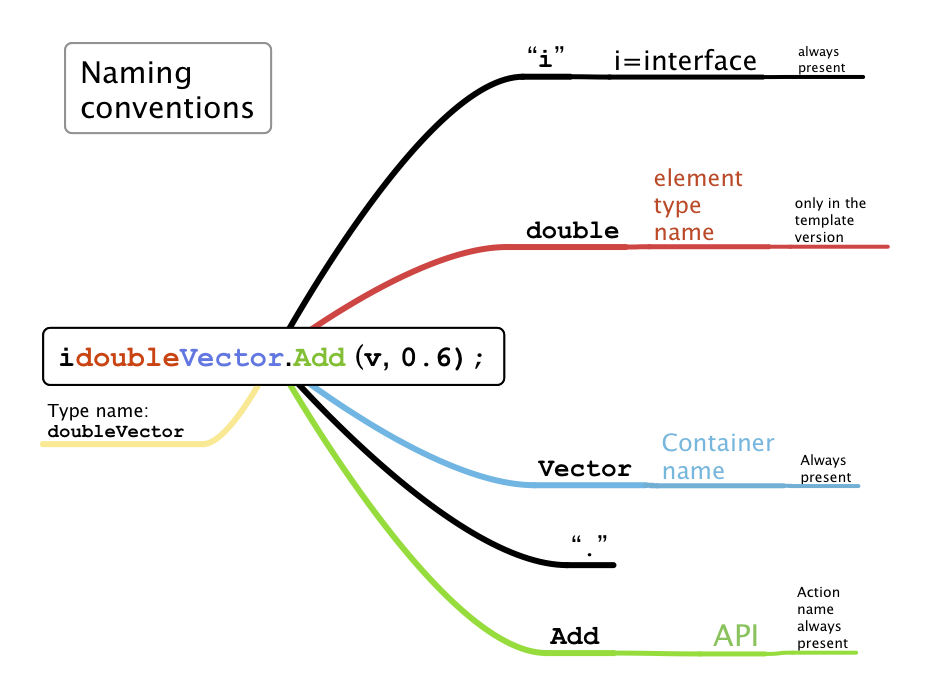
\includegraphics[scale=0.46]{NamingConventions.png}

The different containers built from a basic container (say \verb,List,) are named by concatenating the name of the type and the name of the container:
\verb,intList,, \verb,doubleList, etc.

\section{The different containers}
All data structures in this section are known and used for several decades. Lists are a common feature of any data processing task since the sixties for instance. 
The library provides for abstract containers, and some examples of concrete ones for the elementary types.
We have:
\begin{itemize}
\item
Vectors. The general abstract vector container is implemented in the "Vector" container. This is a flexible array that allows for insertion/deletions, 
with no cost for insertion at the end in most cases. Concrete implementations for the elementary types are provided for bits (bit-strings), strings 
(null terminated), int/double/long double numeric data in the form of templates.

Use this container when you need very cheap traversal and access times. Insertion are deletion are more expensive than in lists. The memory overhead is minimal.

\item
Lists. Single linked lists (List) and double linked lists (Dlist) are provided. Lists of strings and wide character strings are specified too. Memory overhead is one pointer for element in single linked lists, two pointers in double linked lists.

Use this container when you need very cheap insertion and deletion access times. Traversal is more expensive than in vectors.
\item
Queue, Deque, Priority Queue.

Use this containers when retrieval order is important and determined by the container.
\item
Trees (red/black trees, AVL trees)

Use this container when finding a given element is primordial. Insertion, deletions and traversal times are more expensive.
\item
Dictionary. This is a simple implementation of a hash table with character keys. It comes in two flavors\footnote{
Hashtables are present in all major computer languages:
\begin{itemize}
\item C\# features a hash table class that "Represents a collection of key/value pairs that are organized based on the hash code of the key." 
according to the documentation from Microsoft.
\item Java has relatively recently added a HashTable class that "... maps keys to values. Any non-null object can be used as a key or as a value."
\item Fortran doesn't include them in the language itself but there are libraries that implement hash tables in Fortran. For instance 
Herbert J. Bernstein implemented a hash table library in Fortran 2003.
\item In Common Lisp hash tables are standard: \param{make-hash-table} and other functions implement all the needed functionality.
\end{itemize}
They were absent from the C++ STL for unknown reasons. They have been now incorporated into the latest C++ standard.
}
: 
\begin{enumerate}
\item Single byte character keys
\item Wide character keys
\end{enumerate}

Use this container when speed of retrieval is of paramount importance but you want to avoid the overhead of a tree.
\item
Hash Table. More complex implementation of a hash table with arbitrary (binary) keys, and automatic hash table resizing.

Use this container when the key of your dictionary is not in the form of text.
\item Buffers. Stream buffers (linear buffers that resize to accommodate more data) and circular buffers are provided.

Use stream buffers when you need growable temporary data. Use circular buffers when you need to retain the nth last elements of a stream.
\end{itemize}
\subsection{ Single and double linked lists}

\includegraphics[scale=0.63]{SingleLinkedList.png}

This containers consist of a header and a list of elements containing each a pointer to the next element in the chain, and a pointer to the data item 
stored. The end of the list is marked by a node that contains a \Null "next" pointer. Double linked lists contain an additional pointer to the previous 
element.

This is a very flexible container, allowing you to add and delete elements easily just by rewriting some pointers. You can even split them in two 
sublists just by zeroing somewhere the "next" pointer.

The price you pay for this flexibility is that sequential access is expensive, the cost of accessing the nth element increases linearly with n.

Storage overhead is one or two pointers per element stored in the list for single/double linked lists..

The data is stored directly after the pointer, there is no pointer to the data. This is a variable length structure with a fixed and a variable part. 
To avoid using a standard C99 feature that could be absent in older compilers, we use a semi-generic pointer indexed either by one (for older compilers) or by nothing (standard C).

\subsubsection{Single linked lists of byte or wide character strings}
A specialization of the single linked list is provided for multibyte or wide character strings. The rationale for this specialization is that
zero terminated strings are variable length records what would make them impossible to store into a standard list that needs records of the
same size.

\subsection{Flexible arrays (vector)}
This container is an array with added operations that allow the user to insert and delete elements easily. It will resize itself if needed.

The access time is essentially the same as with a normal array. Insertion and deletion are possible but they are in general more expensive than with lists since the container must copy the elements to make place for a new element or to delete an element. An exception to this rule is the deletion of the last element that will be done in constant time since it implies only decrementing the number of elements in the container.

The storage overhead for each element is zero since this container doesn't require any pointers per object stored.

This container uses a reserve storage to avoid allocating new memory for each addition operation. This allows the \verb,Add, operation to be done in constant time in most occasions.

Comparing vectors with plain arrays, there are following points to be made:
\begin{itemize}
\item With plain arrays, a program cannot determine the array's capacity, which is to say, its dimension when it was allocated.  
The program code must supply this information independently, and must maintain that information always current.

\item There isn't any simple way to increase the size of our array, once it’s been allocated.  We often need to do that, rather than try to figure out 
in advance how large it should be.

\item When accessing the array there is no automatic way to check if the index is within bounds. We have to program all array access specially
if we want to make sure there are no index errors.

\end{itemize}

\subsection{ValArray: Arrays of numbers}
This group is an specialization of flexible array. It features objects that contain numbers in different formats designed to facilitate operations
in numerical programming. There are ValArrays for the types \texttt{short}, \texttt{int}, \texttt{long}, \texttt{float}, \texttt{double},
\texttt{long double}, \texttt{size\_t} and \texttt{long long}. Each \texttt{ValArray} has the same basic operations (addition, subtraction, etc)
but some members have specialized operations: trigonometric operations are defined only in floating point ValArrays, boolean operations only in the unsigned versions of the \texttt{int/short} and the \texttt{long long} types.

ValArray functions come often in two flavors: The first uses two arrays where the left argument is both source and destination, and a second form where
a number is applied to the whole array. For instance we have \verb,AddTo(leftArray,\textbf{,}\verb,rightArray), and \verb,AddToScalar(Array,\textbf{,}\verb,number),.
\subsection{String collection}
This container is designed to handle a collection of C strings. It is essentially an application of the flexible array container with some extra functionality to handle strings. It comes in two flavors, as strings in C: multi-byte and wide character strings.
\subsection{Bit-string}
This container is designed to handle arbitrary sequences of bits. Some algorithms that are easy to program with strings are much more complicated for bit-strings, like to one that mimics "strstr" ("bit-strstr"). 

The bits are packed with 8 bits per character unit. The overhead per bit is the size of the bit-string header only. No pointers are associated with each bit.

\subsection{Dictionary}

\includegraphics[scale=0.63]{HashTable.png}

This is an associative container based on a hash table. It associates a text key with some arbitrary data. This container is not ordered. Access time to each element depends on how much elements are stored in it and on the efficacy of the hash function to maintain elements in different slots. Storage overhead per element is one pointer each, plus the size of the slot table. This is for a hash table with linked lists in each slot for managing collisions. Other implementations exist of course.
\subsection{Hash Table}
This is a more sophisticated version of the dictionary hash table. It allows for keys of binary data and it has automatic resizing in case the table gets too crowded.
\subsection{AVL trees}
This data structure allows for fast searching for data. You can store millions of records and find a given record with a few comparisons.
\subsection{Scapegoat trees}
This is another form of trees. They can be more efficient than AVL trees, but from a container perspective they share the same characteristics.
\subsection{Bloom Filter}
This is a probabilistic data structure used to quickly check if an element is not in a larger set of elements. It returns false positives with a given probability set when the container is built. Elements can be added to it but they can't be removed from the container. It stores no data, just a key.
\subsection{Queue}
Queues are designed to operate in a FIFO context (first-in first-out), where elements are inserted into one end of the container and extracted from the 
other. This container can be implemented as an adaptor using a single linked list as its base container. The sample implementation uses this strategy 
to show how adapters can look like. Other implementations can implement this container directly presenting the same interface.
\subsection{Deque}
This is a linear container that allows for cheap insertions/deletions at both ends.
\subsection{Buffers}
Buffers are containers used to hold data temporarily, either to be transmitted or stored into some medium, or to be filtered and used later
by other parts of the application. The library provides two types of buffers:
\begin{itemize}
\item Stream buffers. They are a linear sequence of bytes, like a file. They resize automatically if they need to, and they have a \textsl{cursor}
that points to the position where the next item will be stored.
\item Circular buffers. They store the last \textsl{n} items of a stream. They can contain any item as in the vector container, or they can contain 
character strings, as in the string collection.
\end{itemize}
\subsection{Priority Queues}
This container stores data associated with an integer "priority". The meaning of this integer is not further specified and defined by the application.
The \verb,Pop, operation retrieves the data associated with the \textsl{lowest} priority. 
\subsection{At a glance}
{
\rowcolors{1}{white}{green!8}
\begin{center}
\noindent
\begin{longtable}{||p{3cm}|p{3cm}|p{7.0cm}||}
\hline
\textbf{Container}&\textbf{Interface}&\textbf{Description }\\\hline \hline
BitString&iBitString&Growable array of bits \\
BloomFilter&iBloomFilter&Statistical container \\
CircularBuffer&iCircularBuffer& Circular buffer \\
Deque&iDeque&Double ended queue \\
Dictionary&iDictionary&Hash table with character keys \\
Dlist&iDlist&Double linked list \\
HashTable&iHashTable&Hash tables with arbitrary binary keys \\
List&iList&Single linked list \\
Queue&iQueue&Queue \\
PQueue&iPriorityQueue&Priority queue. \\
StreamBuffer&iStreamBuffer&Stream buffer \\
StringList&iStringList&Single linked list of strings\\
strCollection&istrCollection&Flexible string arrays. \\
TreeMap&iTreeMap&Scapegoat trees \\
Value array&iValArrayXXX&Growable array of numbers \\
Vector&iVector&Growable array of arbitrary objects \\
WstrCollection&iWstrCollection&Flexible array of wide character strings\\
\hline
\end{longtable}
\end{center}
} % end small
%--------------------------------------------------------------------------------------------------------------------------
%                                        THE COMMON VOCABULARY
%--------------------------------------------------------------------------------------------------------------------------
\chapter{The common vocabulary: iGenericContainer}
The library uses always the same words to represent similar actions in all containers. In addition, each container can use specific words to name actions that are specific to it. In this section only the common actions will be documented, to give an overview of the common vocabulary available.

At the end of this documentation you will find a complete table that lists each action supported by the library and marks which container supports it.

\section{Creation of a container: Create}
\index{Create}
Containers are created with a call to their "Create" function.  The first argument is the size of the objects that will be stored in the container. The second is optional and is a hint to the number of elements that will be stored in the container.
Note that if you want to store objects of different sizes you just store a pointer to those objects instead of the objects themselves.
The creation functions can have several arguments, the first being always the size of the elements that the container will hold. The prototype can be:
\begin{verbatim}
Container * iContainer.Create(size_t elementsize,...);
\end{verbatim}
The creation function needs to allocate memory to hold the container. This memory will be allocated using the current memory manager that is always an implicit argument to all creation functions. The rationale behind this design decision is that you don't change your memory allocation strategy at each call to a container creation function. This simplifies the interface at the expense of making the change of allocation strategy more expensive.

There is an abstract class of objects called "Generic container" that has all functions that are common to all containers. This is an abstraction,
and as such, it can't have any concrete examples: there is no creation function for a generic container. You can only create a concrete container, a list, a vector, etc. 

Once created, and if the created container supports the generic interface, you can make a cast and treat the concrete container as an abstract member
of a mythical "generic" container. This can save you a lot of redundant code since your code is independent of the type of container and will run
with any object (even future objects) that support the generic container interface.

\includegraphics[scale=0.4]{Vocabulary.png}\par

As everything, there is no free lunch. Precisely because of its generality the generic interface is missing a lot of functionality that you will find
in the concrete containers interfaces. 

\section{Destruction of a container: Clear and Finalize}
\index{Clear}\index{Finalize}
All containers support two cleanup functions:
	\begin{enumerate}
\item
Clear: remove all elements. The header structure remains untouched. This can be used to free the memory when the container was created with the \texttt{Init} function.
\item
Finalize: Remove all elements and the memory used by the container object using the allocator for this container. The container should NOT have been created using the \texttt{Init} function.
\end{enumerate}
The syntax is:
\begin{enumerate}
\item \texttt{int iContainer.Clear(Container *);}
\item \texttt{int iContainer.Finalize(Container *);}
\end{enumerate}
The result of those functions is less than zero when something goes wrong, greater than zero otherwise.
\subsection{Other creation functions}
\begin{enumerate}
\item
An implicit argument to all the creation functions is the current allocator, that is used to retrieve space for the container being built. To avoid changing the current allocator, what in multi-threaded environment would need acquiring a lock to that global variable, some containers support a creation function that receives an extra argument: a custom allocator.
\begin{verbatim}
Container * iContainer.CreateWithAllocator(size_t elementsize,
                     const ContainerAllocator *allocator, ...);
\end{verbatim}
\item
Sometimes it can be useful for some containers (specially lists) to create the  header structure using an already existing space, for instance in the space for local variables. For this an 'Init' function can exist, that initializes a container within an existing space.
Since normally the detailed structure (and the size of course) of each container header is implementation dependent, you use the Sizeof function with an argument of \Null to get the size of the header. This can be used within a C99 compiler environment to allocate the space for that variable.
\footnote{This incredibly useful feature has been made now optional by the C99 committee, even if it was mandatory when the C99 standard was published.}
The declaration of the container header in C99 would be:
\begin{verbatim}lc tta
int function(void)
{
    char listSpace[iList.Sizeof(NULL)];
    iList.Init(listSpace);
}
\end{verbatim}

If C99 is not available, the best way is to just print the size of the container you are interested in, and then use that value that should stay fixed 
for a given version. This can be automated and you can find in the Appendix 1, a small program that generates a series of \texttt{\#defines} with the 
values of the sizes of the containers described in this documentation.

Problems with the above construct could arise because of the alignment requirements of the platform 
where the library is running. Instead of a \verb,char, as the type
of the buffer, it is better to use a slightly more complicated expression to ensure correct alignment. For instance:
\begin{verbatim}
    size_t s = (sizeof(void *)-1+iList.Sizeof(NULL))/sizeof(void *);
    void *listSpace[s];
\end{verbatim}

\footnote{
Other frameworks use a similar method. For instance Apple Foundation classes has several classes that take an "allocator" argument, for instance the
\texttt{CFBundleCreate} and other functions that create objects.
}.

\item Initializing with existing data
All containers support the \verb,InitializeWith, function. It will create a container using a table of elements to store. Its arguments are the size of 
the objects to be stored, the number of those objects, and a pointer to the table. The table should be a contiguous memory area.
\begin{verbatim}
/* For sequential containers and TreeMap */
Container * iContainer.InitializeWith(size_t elementsize,
                              size_t n, void *data);
/* For Dictionary */
Container * iContainer.InitializeWith(size_t elementsize,
                              size_t n, char ** Keys,void *data;
\end{verbatim}


\end{enumerate}
\section{Adding an element to a container: Add and AddRange}
This operation adds the given element to a container. In sequential containers it is added at the end, in associative containers it is added at an unspecified position.
\begin{verbatim}
int iContainer.Add(Container *,const  void *element);
\end{verbatim}
The result of this operation is a positive integer if success, or an error code less than zero if the operation fails.
\Const The input data is not modified in any way, it is copied into the container.

Sequential containers support also the \texttt{AddRange} API:
\begin{verbatim}
int iContainer.AddRange(Container *,size_t n,const void *elements[]);
\end{verbatim}
This API allows you to pass a table of elements into a sequential container and add it with a single call.
\section{Removing elements from a container}
\subsection{Using an element as key}
The functions \texttt{Erase} and \texttt{EraseAll} remove the given element from the container. 
The result is an integer greater or equal to zero or an error code less than zero if the element couldn't be added
\footnote{In previous versions these functions returned some useful information in case of success, for instance the number of elements left. The problem is that an int can't span all the possible values of a \texttt{size\_t} data type but it is needed to return negative
error codes. If the result type would be a \texttt{size\_t} the negative error codes would be transformed in other values, etc. After some iterations 
the present solution was used: a positive number is equal to success, without specifying what the positive number is, or what information (if any) 
should be coded in it. The sample implementation always returns 1.} 
.

The \texttt{EraseAll} function is not needed for associative containers since each element in those data structures is unique.
\begin{verbatim}
int iContainer.Erase(Container *,const void *element);
int iContainer.EraseAll(Container *,const void *element);
\end{verbatim}
\subsection{Removing at a given position}
\noindent The \texttt{Erase/EraseAt} functions need to search for the given element before erasing it. For sequential containers you can use the "EraseAt" function, that will remove an element at a given position.
\begin{verbatim}
int iContainer.EraseAt(Container *,size_t idx);
\end{verbatim}
\noindent
For associative containers you use a different argument set:
\begin{verbatim}
int iContainer.Erase(Container *,const char *Key);
\end{verbatim}
\subsection{Using a container as a stack}
Elements can be removed from the front or the back in sequential containers using it like a stack:
\begin{verbatim}
int iContainer.PopBack(Container *d,void *outbuf);
int iContainer.PopFront(Container *d,void *outbuf);
\end{verbatim}
These functions copy the contents of the last or the first element into the given buffer. If the buffer is NULL, nothing is copied, but the
container is modified: the first or the last element is removed.
\subsection{Batch removing}
Several elements can be removed at once from a container using the \texttt{RemoveRange} function. This function is implemented in sequential
containers only.
\begin{verbatim}
int iContainer.RemoveRange(Container *c,size_t start, size_t end);
\end{verbatim}
This function removes the elements whose index is greater or equal than \textsl{start} and less than \textsl{end}. If \textsl{start} equals \textsl{end}
nothing is removed and the result is zero. If \textsl{end} is greater than the length of the container it will be adjusted to 1 element past the
end. If no elements are removed the result is zero, positive when one or more elements are removed. The result is a negative error code when an
error occurs.

\section{Retrieving elements}
The GetElement function retrieves an element from a container. It comes in two different flavors, one for sequential containers, and another for associative ones.
\begin{verbatim}
const void *iContainer.GetElement(const Container *,size_t index);
const void *iContainer.GetElement(const Container *,const void *Key);
\end{verbatim}
These functions return a pointer to the requested element or \Null if the element can't be retrieved. The resulting pointer points directly to the data 
stored in the container. This could be used to bypass all the flags that control the access to the container. For read-only containers, use the 
\texttt{CopyElement} function that returns a copy of the requested data into a buffer.

The function \texttt{GetRange} retrieves a slice of a container returning a container of the same type with a copy of the elements stored in the
given range: \index{GetRange}
\begin{verbatim}
Container *iContainer.GetRange(const Container *src,
                              size_t start, size_t end);
\end{verbatim}

The pointer returned can be invalidated by some operations done to the container. For instance if you reverse the order of the elements in a container, 
a pointer to the element zero will point to something else than when you obtained it. If a container needs reallocating its data space because you
added an element, all the pointers that point to data elements of the container can be invalidated. In general \textbf{it is a bad idea to keep pointers 
to elements in a container that is being modified}
\Const The given container is not modified in any way.
\section{Using masks}
A \verb,mask, is a sequence of boolean elements that contains zeroes or some value different from zero. They are used to select elements from a sequential container: for each element of the mask different from zero the corresponding value is selected, for all elements that contain a zero, that value is eliminated.

The selection operation can be destructive, reusing a container by eliminating from it all elements not selected by the mask, or can be a copy operation where the copy contains only the selected elements.

In the case of a destructive operation, the destructor functions are called for each element destroyed.
\begin{verbatim}
int (*Select)(Container *,const mask *);
Container *(*SelectCopy)(const Container *,const mask *);
\end{verbatim}

The functions \verb,CompareEqual, and \verb,CompareEqualScalar, produce a mask using two containers as input. Those masks can be used with the selection functions. It is possible of course, to create masks from completely different sources, either directly or by copying. See the \verb,iMask, interface for further details.

\begin{verbatim}
Mask *(*CompareEqual)(const Container *,const Mask *);
Mask *(*CompareEqualScalar)(const Container *, const Mask *);
\end{verbatim}


The \verb,CompareEqual, function compares two sequential containers of the same type and length, producing a mask containing a value different from zero at each element position where the pair of elements from each container is equal, zero otherwise.

The \verb,CompareEqualScalar, function compares each element of the given sequential container with a single element, producing a mask with a value 
different from zero\footnote{Usually this value is 1 of course} for each element that is equal to the given element.
\section{Sorting a sequential container: Sort}
The "Sort" function will sort a container in place. To keep the old, unsorted contents, make a copy of the container first.
\begin{verbatim}
int iContainer.Sort(Container *);
\end{verbatim}
\section{Copying a container: Copy}
\noindent The "Copy" function will make a fresh copy of a container. Some fields of the header are copied: the error and compare functions, the flags, and others. Memory will be allocated withe the source container allocator.
\begin{verbatim}
newContainer * iContainer.Copy(const Container *);
\end{verbatim}
\Const The input container is not modified.
\section{Saving and loading a container to or from disk: Save and Load}
The functions "Save" and "Load" will save / load the contents, state, and characteristics of a container into / from disk. They need an open file stream, open in binary mode, and in the correct direction: saving needs a stream open in the write direction, loading needs a stream open in the read direction.
\begin{verbatim}
int Save(const Container *c,FILE *stream, SaveFunction fn,void *arg);
Container *Load(FILE *stream,ReadFunction fn,void *arg);
\end{verbatim}
Both \texttt{Save} and \texttt{Load} provide default functions to save and load an element but they do a \textsl{shallow} save: pointers aren't followed 
to save the data they point to \footnote{In general it is a bad idea to save elements containing pointers without a custom save/load function. The 
pointers restored are with almost certainty wrong when restored in another environment}.
\section{Inserting a container into another}
\subsection{Sequential containers}
\noindent
\begin{verbatim}
int (*InsertIn)(Container *destination,
                size_t position,
                Container *source);
int (*Append)(SequentialContainer * SC1,SequentialContainer * SC2);
\end{verbatim}
The \texttt{InsertIn} function will insert into the "destination" container the contents of the \verb,source, container at the given position. The source is not modified in any way, and a copy of its data will be used. Both containers must be of the same type and store elements of  the same type. The library only tests the element size of each one.

The \texttt{Append} function is similar to InsertIn: the elements of the second container are appended at the end of the first one. The big difference 
is that the second container is destroyed. It is absorbed into the first: its elements are not copied but inserted. This means that a requirement is
that the allocator be the same in both containers.
\subsection{Associative containers}
\begin{verbatim}
int (*InsertIn)(Container *destination, Container *source);
\end{verbatim}
This function will insert into the destination container the source container using the source container keys. Otherwise the same conditions apply as to the sequential containers: the containers must be of the same type and store elements of the same type.
\section{Replace an element with another}
\subsection{Sequential containers: ReplaceAt}
\begin{verbatim}
int (*ReplaceAt)(Container *dst,size_t position,void *newData);
\end{verbatim}
Replaces the element at the given position with the new data. 
\subsection{Associative containers: Replace}
\begin{verbatim}
int (*Replace)(Dictionary *Dict, const char *Key,void *Value);
\end{verbatim}
Replaces the element with the given key. If the element is absent nothing is done.
\section{Looping through all elements of a container}
The user has  three methods for looping through all elements:
\begin{enumerate}
\item Using a simple loop construct
\item Using the \verb,Apply, function
\item Using an iterator
\end{enumerate}
One the most familiar design patterns  is the ITERATOR pattern, which ‘provides a way to access the elements of an aggregate object sequentially without exposing its underlying representation. 

Traditionally, this is achieved by identifying an ITERATOR interface that presents operations to initialize an iteration, to access the current element, to advance to the next element, and to test for completion; collection objects are expected to implement this interface, usually indirectly via an auxiliary object. 

This is exactly the case in the iterator proposal here. Essential to the pattern is the idea that elements are accessed sequentially, but independently of their position in the collection; for example, labeling each element of a tree with its index in left-to-right order fits the pattern, but labeling each element with its depth does not. This traditional version of the pattern is sometimes called an EXTERNAL ITERATOR. 

An alternative INTERNAL ITERATOR approach assigns responsibility for managing the traversal to the collection instead of the client: the client needs only to provide an operation, which the collection applies to each of its elements. The latter approach is simpler to use, but less flexible; for example, it is not possible for the iteration to affect the order in which elements are accessed, nor to terminate the iteration early. This is the algorithm followed by the \verb,Apply, function.

\subsection{Using a simple loop to iterate a container}

You can iterate any sequential container with a simple loop. You use the "Size" function to limit the loop. At each loop step you get the corresponding 
element with the "GetElement" function, present in this form in all containers.
\begin{verbatim}
// "Container" is a pointer to some container
for (size_t i=0; i<iContainer.Size(Container); i++) {
    someType *element = iContainer.GetElement(Container,i);
    // Use "element" here.
}
\end{verbatim}
For associative containers you retrieve first a strCollection containing all keys using the \texttt{GetKeys} function, present in all associative 
containers. Then, you retrieve each element by looping through the string collection that you have obtained in a similar manner to the sequential 
containers. 

\subsection{Using the Apply function.}
\index{Apply!general}
The \verb,Apply, function will iterate through all elements calling a given function for each one.1 Its prototype is:
\begin{verbatim}
void iContainer.Apply(Container, //pointer to some container
                      int(*Applyfn)(void *elem,void *arg),
                      void *arg);
\end{verbatim}
This function receives three arguments:
\begin{enumerate}
\item A pointer to the container. \footnote{Note that the container is not declared as \texttt{const} and could possibly be modified either directly or 
indirectly by the function being applied to it. Some modifications like modifying the number of elements could lead to undefined behavior since it
is not required that the Apply loop tests at each iteration if the container has been modified}.
\item A function pointer that should point to a function that receives two arguments: the element of the container, and an extra argument where it can 
receive (and write to) global information about the search.  This extra argument is 
\item The third one passed to the \verb,Apply, function. \verb,Apply, will pass this argument to the given function together with a pointer to the 
element retrieved from the container.
\end{enumerate}
\subsection{Using iterators}
\index{Iterators!General}
Iterators are objects returned by each container that allow you to iterate (obviously) through all elements of a container.
You use iterators like this:
\begin{verbatim}
Iterator *it = iContainer.NewIterator(someContainer);
Mytype *myobject;
for (myobject = it->GetFirst(it); 
     myobject!= NULL; 
     myobject = it->GetNext(it)) {
     // Work with "myobject" here
}
iContainer.DeleteIterator(it); // dispose the iterator object
\end{verbatim}
Iterators provide a container-independent way of iterating that will work with any container, both sequential or associative. In associative containers 
the specific sequence is implementation defined, and in sequential containers is the natural sequence.

The main objective for iterators is to break a dependence between an algorithm and the type of container it is working with. Since all containers
support iterators, you can write your code independently (to a great extent) from which specific iterator you are using.
\Const The input container could be modified in some implementations. A list of existing iterators is possible, to allow invalidating them in case of
modifications to the container for example.

Iterators always support at least the following functions:
\begin{verbatim}
void *iterator->GetFirst(iterator);
void *iterator->GetNext(iterator);
void *iterator->GetCurrent(iterator);
\end{verbatim}
All containers support the "NewIterator"  and "deleteIterator" methods:
\begin{verbatim}
iterator *iContainer.NewIterator(Container); 
int iContainer.deleteIterator(iterator);
\end{verbatim}
Iterators must be destroyed since they are allocated using the containers allocator.

Sequential containers can support additional functions:
\begin{verbatim}
void *iterator->GetLast(iterator);
void *iterator->GetPrevious(iterator);
void *iterator->Seek(iterator i, size_t position);
\end{verbatim}
This interface allows users to write fully general algorithms that will work with any container, independently of its internal structure. Obviously the 
performance can differ from container to container depending on usage.

All iterators will become invalid if the underlying container changes in any way, except through the iterator itself.\footnote{This is completely 
different to the C++ language. In C++ you may have an invalid iterator or not if you change the underlying container, depending on the 
operation and the specific container involved. This interface was discarded for the following reasons:
\begin{enumerate}
\item There are many rules to remember without underlying principles.
  You have to know the specifics of each container to know
  if the iterators are invalidated or not. This breaks the independence
   of the algorithm code from the underlying container.

\item Any error leads directly to catastrophic consequences instead
   of being caught and signaled in an orderly fashion. Worst, errors
   do not produce always the same consequences, depending on what
   were the contents of the invalid memory you are using, on the
   memory allocation pattern, etc. In short, any error leads to
   very difficult maintenance problems.

\item Any modifications of the container type lead to a review of
   all code that uses that container since the rules change from
   container to container. Iterators that worked could be invalid
   now. This another source of errors.
\end{enumerate}
}
Each container can conceptually be seen as a sequence of \textsl{generations}, or \textsl{states}. Beginning with the fresh constructed state, the container
evolves until it reaches the destroyed state after the execution of the \verb,Finalize, function. This sequence of states interacts with an
iterator as follows: An iterator applies only to a \textbf{single} container state. Any modification of the container state, directly or
indirectly moves the state and invalidates the iterator.

An implementation may catch some of the movements of the container in the state space and report an error when an iterator is used that belongs to 
a different container state. But not all access can be detected. If the user has pointers to an iterator's data and modifies this data without
using the container API an implementation may not catch this error.

\section{Setting and retrieving the state: GetFlags and SetFlags}
Each container has a set of flags that can be read and written to change the container's behavior. The only flag that is defined by all containers
is the read-only flag. Implementations can extend this to offer different services like copy-on-write, or other applications. 

The read-only flag means that no direct pointers to an element or to the whole data are returned, no functions that modify the
container are allowed to proceed and that the \verb,Clear(),
and \verb,Finalize(), APIs will not work. You must unset this flag to allow for destruction of the object.
\footnote{Contrary to C++ \texttt{const} directive this is done at run time and an explicit check of this flag is needed. This has disadvantages 
(one instruction and a conditional jump are needed) but it has also advantages: you can set it when you pass some container to another module, and unset it when you need to update the container. This solution is more flexible than the static solution at the cost of a very small runtime cost.}

Using the state space concept introduced above, this flag freezes the state of a container disallowing any further evolution. The only API that
can modify the state is the \verb,SetFlags, API that can reset the state to a read/write state again.
\section{Retrieving the number of elements stored: Size}
\index{Size}
All containers support querying the number of elements stored. The prototype is:
\begin{verbatim}
    size_t iContainer.Size(const Container *);
\end{verbatim}
There is no error return. If a \Null pointer is given to those functions the result is zero.
\section{Sizes}
\subsection{Sizeof}
This computes the total size used by the container in bytes, including the header structure and the data stored in the container. Any other overhead 
must be accounted for.
\begin{verbatim}
    size_t iContainer.Sizeof(const Container *);
\end{verbatim}

If its argument is \Null, \texttt{Sizeof} returns the size of the container header. This can be used to allocate space for a container as a local variable for instance.

\subsection{SizeofIterator}
\index{SizeofIterator}
Computes the size of the iterator for the given container. The objective here is to allow the declaration of the iterator as a local variable
to avoid having to free the iterator at the exit of the function.
\begin{verbatim}
int Fn(void)
{
    char buf[iList.SizeofIterator(NULL)];
    Iterator *it = (Iterator *)buf;
    iList.InitIterator(it);
    // Use iterator "it" here
    // ...
    // No need to call deleteIterator at exit
}
\end{verbatim}

\section{Memory management}
\index{Allocator}
All containers have a pointer to their allocator object. An allocator object is a simple interface that provides 4 functions:
\begin{enumerate}
\item malloc: A function that receives a \texttt{size\_t} and returns a \texttt{void *} pointing to a memory block of the requested size, or \Null if no more memory is available. Note that this function receives the number of \textbf{bytes} to allocate, not the number of items.\footnote{In C++ the allocator receives the number of items to allocate.}
\item realloc: A function that will resize a previously allocated block.
\item free: A function that will release the memory allocated previously with malloc/realloc.
\item calloc: a function that will allocate \verb,n, objects of \verb,m, size and clear the memory block to zero before returning it. 
\end{enumerate}
At the start of the library runtime a default allocator object exists that uses the four functions of the standard C library. Other allocator objects can be used, and the user can change the global allocator at any time. Each container retrieves the default allocator object when created, and stores it in the container descriptor. Any further change to the default allocator will not affect existing containers that have already an allocator. When changing the allocator you should do that before creating the container.
 
Some containers are created without any heap management by default. You can introduce heap management by calling the \verb,UseHeap, function, that will install a new heap in the container. Other containers are always created with a heap, and you should pass them an allocator object for object creation.

\subsection{Memory manager objects}
The library provides two memory manager objects:
\begin{enumerate}
\item The default memory manager, that receives the standard C library functions; malloc, free, realloc and calloc.
\item The debug memory manager that implements the same functions with added functionality designed to:
\begin{itemize}
\item
Catch the "double free" problem.
\item
Catch the overflow of a memory block
\item
Catch freeing a block that wasn't allocated
\end{itemize}
\end{enumerate}
\subsection{Pooled memory management}
The problem with the traditional C memory management is that it requires that the programmer cares about each piece of RAM that is allocated by the program and follows the lifetime of each piece to ensure that it gets returned to the system for reuse. In today's software world, this is just impractical.

A better strategy is to use a pool of memory where related memory allocations can b e done from a common pool. When the module finishes, all the allocated pool is freed just by destroying the whole pool. This is much easier to manage, and in many cases more efficient.
The proposed interface has the following functionalities:
\begin{enumerate}
\item Creation. The creation function receives a memory allocator to use for this pool.
\item Alloc. This function receives a pool and a size and returns a memory block, or \Null if there is no more memory.
\item Clear. This erases all objects allocated in the pool without returning the memory to the system.
\item Finalize. This releases all memory and destroys all objects.
\end{enumerate}
Note that there is no realloc, and that the "Clear" function is optional. Not all pools support it. The rationale for these decisions being that realloc would need to store the size of each block, what in a pool maintained by a single stack like pointer would be very expensive.
\subsection{Heap of same size objects}
Many containers are used to store sets of objects of the same size. The library provides a specialized heap management software for this application. It stores vectors of objects of the same size. The interface provided is as follows:
\begin{itemize}
\item Create. This function receives as an argument a memory manager object that will be used to allocate memory.
\item NewObject: returns an object to the application
\item FreeObject: Adds an object to the list of available objects
\item Size: Returns the size of the heap in bytes
\item Clear: reclaims memory used by the free list
\item Finalize: Reclaims all memory used by the heap and the heap object
\end{itemize}

\subsection{Garbage collection}
Automatic garbage collection is offered by some compiler systems as an alternative to traditional memory management. This solution is
not compatible with real time requirements, and is not practical in machines with very low memory configurations.

In other cases however, it can be a real simplification since the programmer is relieved from the huge task of taking care of each
piece of memory and to cater its disposal. A simple memory model is proposed: you program as if the amount of memory was infinite
and never worry about freeing the memory you use. Periodically the collector starts collecting unused memory chunks and adds them
to the pool of available memory or releases it to the underlying operating system.

This model is not the solution to all memory management problems. It can be a solution to some situations, specially when developing
in workstation environments where memory is freely available. The bugs that can appear are also very difficult to solve. One of the
most difficult is when you keep by mistake some reference to a large piece of memory making the recycling of the memory impossible.
In that case you have to search in all the code of the application for the reference that keeps the memory block marked as used, and that can
be very difficult in large applications.
\subsection{Multi-threading}
In environments where multi-threading or other parallel programming constructs are possible, the implementation must provide for sequential
semantics, i.e. each operation should perform as described in this documentation with the additional caveat that any operation that modifies
a container must be \texttt{atomic}, i.e. it can't be interrupted leaving the container in an unstable or incoherent state. It is up to the
implementation to ensure that if an atomic operation is interrupted, the inconsistent container state will be invisible to other processes
or threads accessing the container.
\section{At a glance}
For a more detailed description \See{APIOverview}
{\footnotesize
\begin{longtable}{|p{3.5cm}|p{10.5cm}|}
\hline
\textbf{Operation}&\textbf{Description}\\\hline 
Add&Adds a single element at the end of the container\\\hline
AddRange&Adds a sequence of elements\\\hline
Append&Adds a container after a first one \\\hline
Apply&Calls a function with each element of the container in  sequence.\\\hline
Clear&Erases all elements \\\hline
Contains&Searches for an element in a container\\\hline
Copy&Copies a container \\\hline
Create&Creates a container that will use the current allocator.\\\hline
CreateWithAllocator&Creates a container that will use a given allocator.\\\hline
deleteIterator&Disposes of the storage used by the iterator object \\\hline
Equal&Compares two containers of the same type \\\hline
Erase&Removes an element from the container\\\hline
EraseAt&Erases an element at a given position \\\hline
Finalize&Destroys all storage used \\\hline 
GetElement&Retrieves one element from a container \\\hline
GetFlags&Returns the flags\\\hline
GetAllocator&Retrieves the allocator used by the container\\\hline
GetRange&Retrieves several elements\\\hline
IndexOf&Retrieves the position of an element \\\hline
InsertAt&Inserts an element at a given position \\\hline
InsertIn&Inserts a container into another \\\hline
Load&Retrieves a container from disk \\\hline
NewIterator&Returns an iterator object \\\hline
PopFront & Retrieves the first element and removes it\\\hline
PopBack& Retrieves the last element and removes it\\\hline
PushFront & Stores an element at the start of a container\\\hline
PushBack& Stores an element at the end \\\hline
RemoveRange&Erases a range of elements \\\hline
Replace & Replaces one element (Associative containers)\\\hline
ReplaceAt & Replaces one element (Sequential containers) \\\hline
Save&Stores the container to disk \\\hline
SetCompareFunction&Sets or retrieves the function used for comparisons \\\hline
SetErrorFunction&Sets or retrieves the function used to report errors\\\hline
SetDestructor&Sets or retrieves the function called when an element is destroyed \\\hline
Select&Selects elements using a mask \\\hline
SelectCopy&Select elements to copy using a mask.\\\hline
SetFlags&Sets the flags\\\hline
Size&Returns the number of elements stored in the container \\\hline
Sizeof&Returns the number of bytes used \\\hline
SizeofIterator&Returns the size of the iterator object for a container \\\hline
Sort&Sorts the contents \\\hline
 
\multicolumn{2}{|c|}{ \textbf{Iterator vocabulary}} \\\hline
GetFirst & Retrieves a pointer to the first element\\\hline
GetNext & Retrieves a pointer to the next element \\\hline
GetPrevious & Retrieves a pointer to the previous element if the container supports bidirectional seek.\\\hline
GetCurrent& Retrieves a pointer to the current element \\\hline
GetLast & Retrieves a pointer to the last element \\\hline
Replace & Replaces the current element with a different element. If the given pointer to the replacement is \Null 
it will delete the current element.\\\hline
Seek& Sequential containers only. Positions the cursor at a given position.\\\hline
\end{longtable}
} % end footnotesize above
%--------------------------------------------------------------------------------------------------------------------------
%                                                   INTERFACES
%--------------------------------------------------------------------------------------------------------------------------
\chapter{The auxiliary interfaces}
These interfaces are used by all the containers in the rest of the library. They provide basically the following functions:
\begin{itemize}
\item Memory management with the \texttt{Allocator} object.
\item Observer and circulation of notifications with \texttt{iObserver}.
\item Error handling with the \texttt{iError} interface.
\item Masks used to select items
\end{itemize}
\includegraphics[scale=0.63]{Basic.png}
\section{Masks}
A mask is a sequence that contains boolean data used for selection of items in a sequential container. 
It is not specified if a mask is a bit string (i.e. a
strictly boolean array) or an array of chars or other integers used to hold the binary data. In all cases a value of the mask at a given position 
means \textsl{select} if it is different than zero, or \textsl{do not select} if it is zero.

The interface offered by the mask object is very small. Masks can't be resized but they have an allocator to be able to reclaim the
memory they use when created. This allocator will be initialized to the current allocator when the mask is created.
\subsection{The interface}
\begin{verbatim}
typedef struct _Mask Mask;
typedef struct tagMaskInterface {
    int (*And)(Mask *src1,Mask *src2);
    int (*Clear)(Mask *m);
    Mask *(*Copy)(Mask *src);
    Mask *(*Create)(size_t length);
    Mask *(*CreateFromMask)(size_t length,char *data);
    int (*Finalize)(Mask *m);
    int (*Or)(Mask *src1,Mask *src2);
    size_t (*PopulationCount)(const Mask *m);
    int (*Set)(Mask *m,size_t idx,int val);
    size_t (*Size)(Mask *);
} iMask;
\end{verbatim}
\subsection{The API}
\api{And}
    int (*And)(Mask *src1,Mask *src2);
\end{verbatim}
\apidescription
Stores into src1 the result of a logical AND operation between each element of src1 with the corresponding element of src2.
\apierrors
\doerror{BADARG} Any mask pointer is \Null.
\doerror{INCOMPATIBLE} The masks are of different length.
\returns
A positive number if the operation was performed, a negative error code if an error occurs.
\api{Clear}
    int (*Clear)(Mask *m);
\end{verbatim}
\apidescription
Sets all elements of the mask to zero.
\apierrors
\doerror{BADARG} The mask pointer is \Null.
\returns
A positive number if the mask was cleared, a negative error code if an error occurs.
\api{Copy}
Mask *(*Copy)(Mask *src);
\end{verbatim}
\apidescription
Allocates a new mask and copies the contents of the given one into it.
\apierrors
\doerror{BADARG} The mask pointer is \Null.
\returns
A pointer to the new mask or \Null if an error occurs.

\api{CreateFromMask}
    Mask *(*CreateFromMask)(size_t length,char *data);
\end{verbatim}
\apidescription
Creates a new mask with the specified length and copies the given data into the mask. Each character in the input data is transformed into the
mask internal representation. The storage is obtained using the CurrentAllocator pointer.
\apierrors
\doerror{BADARG} The data pointer is \Null
\doerror{NOMEMORY} No memory is available to perform the allocation.
\returns A pointer to a new mask or \Null if an error occurs.

\api{Create}
    Mask *(*Create)(size_t length);
\end{verbatim}
\apidescription
Creates a new mask with the specified length. The storage is obtained using the CurrentAllocator pointer. The data is initialized to zero.
\apierrors
\doerror{NOMEMORY} No memory is available to perform the allocation.
\returns A pointer to a new mask or \Null if an error occurs.

\api{Finalize}
    int (*Finalize)(Mask *m);
\end{verbatim}
\apidescription
The memory used by the mask is reclaimed.
\apierrors
\doerror{BADARG} The mask pointer is \Null.
\returns A positive number if the memory was reclaimed, or a negative error code.

\api{Not}
    int (*Not)(Mask *src);
\end{verbatim}
\apidescription
Stores into src the result of a logical NOT operation: each bit is inverted.
\apierrors
\doerror{BADARG} The mask pointer is \Null.
\returns
A positive number if the operation was performed, a negative error code if an error occurs.


\api{Or}
    int (*Or)(Mask *src1,Mask *src2);
\end{verbatim}
\apidescription
Stores into src1 the result of a logical OR operation between each element of src1 with the corresponding element of src2.
\apierrors
\doerror{BADARG} Any mask pointer is \Null.
\doerror{INCOMPATIBLE} The masks are of different length.
\returns
A positive number if the operation was performed, a negative error code if an error occurs.

\api{PopulationCount}
   size_t (*PopulationCount)(const Mask *m);
\end{verbatim}
\apidescription
Counts the number of entries different from zero in the given mask, returning the sum.
\apierrors
\doerror{BADARG} The mask pointer is \Null.
\returns
A positive number or zero.


\api{Set}
    int (*Set)(Mask *m,size_t idx,int val);
\end{verbatim}
\apidescription
Sets the given position to the given value if the value fits in the internal representation of the mask. If not, an implementation defined
conversion occurs.
\apierrors
\doerror{BADARG} The mask pointer is \Null.
\doerror{INDEX} The index given is out of bounds.
\returns A positive number if the value was set or a negative error code.

\api{Size}
    size_t (*Size)(Mask *);
\end{verbatim}
\apidescription
The number of elements in the mask is returned.
\apierrors
\doerror{BADARG} The mask pointer is \Null.
\returns The number of elements. If the mask pointer is \Null, the result is zero.

\api{Sizeof}
    size_t (*Sizeof)(Mask *);
\end{verbatim}
\apidescription
The number of bytes used by the given mask. If the argument is \Null the number of bytes of the header structure is returned.
\apierrors
None.
\returns The number of bytes.

\section{Memory management}
Several interfaces implement different memory allocation strategies. This should give flexibility to the implementations, allowing it to use several memory allocation strategies within the same container.\par
The library starts with the \texttt{default} memory manager, that contains pointers to the default C memory management functions: malloc, free, realloc and calloc. Another memory manager is the \texttt{debug} memory manager that should implement more checking and 
maybe offer hooks to the debugger. The sample
implementation shows how to implement several simple checks, but other implementations can extend this simple interface providing 
much more sophisticated controls\footnote{An open issue is whether the interface of the memory allocator should be extended with functions like
\texttt{GetSize} for instance, that would return the size of a given memory block, or other query functions like \texttt{isMallocBlock} that would
allow to verify if a memory block belongs to the pool. Some proposals were discussed in the discussion group \texttt{comp.std.c} but nothing official
has emerged from the committee meetings}.

\includegraphics[scale=0.45]{MemoryManagement.png}\par
\subsection{The default memory manager}
The C language provides several functions to manage memory. The default Allocator object is built from the standard C memory allocation functions.
\begin{verbatim}
typedef struct tagAllocator {
    void *(*malloc)(size_t);
    void  (*free)(void *);
    void *(*realloc)(void *,size_t);
    void *(*calloc)(size_t,size_t);
} ContainerAllocator;
extern ContainerAllocator * CurrentAllocator;
\end{verbatim}
At startup, the CurrentAllocator points to an object constructed with the functions of the C standard library. This is a required interface.
The user can change at any time the current allocator by making the \verb,CurrentAllocator, point to a different object. Note that this change
does \textbf{not} change the allocators of the containers already created but the allocators of the new containers allocated after the
change is made.

This is the established procedure to build custom memory allocators to provide for special alignment requirements, improve speed, allocate objects
from the stack instead of the heap, and many other usages.

All containers have an \verb,Allocator, object, either explicitly when created with the \verb,CreateWithAllocator, API or implicitly since all 
creation functions use the object pointed to by the \verb,CurrentAllocator, global variable to obtain memory.

The library can also include a debug version on top of the standard C functions, offering the same interface. Changing the CurrentAllocator to point to that object allows to switch to the debug version. The debug version of the sample implementation offers:
\begin{itemize}
\item
Detection of free() of a memory block not allocated by malloc().
\item
Detection of  writing past the end of the block in some cases.
\item
Detection of freeing a memory block twice.
\end{itemize}
\begin{verbatim}
extern ContainerAllocator iDebugMalloc;
\end{verbatim}
This interface is optional. The sample implementation documents a possible implementation, \See{Malloc}.

\subsubsection{Interface for modifying the current allocator}
\begin{verbatim}
typedef struct tagAllocatorInterface {
    ContainerAllocator *(*Change)(ContainerAllocator *newAllocator);
    ContainerAllocator *(*GetCurrent)(void);
} AllocatorInterface;
extern AllocatorInterface iAllocator;
\end{verbatim}
\renewcommand{\container}{Allocator}
\api{Change}
    ContainerAllocator *(*Change)(ContainerAllocator *newAllocator);
\end{verbatim}
\apidescription Changes the value pointed by the \verb,CurrentAllocator, pointer to the given one. This is an atomic operation. If the given 
allocator pointer is \Null nothing is changed.
\apierrors
None
\returns The old value stored in the \verb,CurrentALlocator, pointer.
\api{GetCurrent}
    ContainerAllocator *(*GetCurrent)(void);
\end{verbatim}
\apidescription Returns the value pointed to by the \verb,CurrentAllocator, pointer. This operation is atomic.
\returns The value stored in the ,CurrentAllocator, pointer
\footnote{This API exists to provide a portable entry point for implementations that support threads of execution or parallel environments. 
Implementations where those features do not exist can recommend user to directly modify the value of the \verb,CurrentAllocator, pointer for
efficiency reasons.
}
.

\subsection{The Heap interface: iHeap}
\renewcommand{\container}{Heap}
Some containers can benefit from a cacheing memory manager that manages a stock of objects of the same size. This is not required and not all implementations may provide it. If they do, the interface is:
\begin{verbatim}
    int (*UseHeap)(Container *c);
    ContainerHeap *(*GetHeap)(Container *c);
\end{verbatim}
In the sample implementation, many complex data structures are implemented using a heap. This allows automatically to have an iterator, since for 
looping all elements of the container it suffices to iterate the underlying heap.
The standard interface for the heap is:\index{iHeap}
../texdoc/ContainerHeap.tex
\api{Create}
ContainerHeap *iHeap.Create(size_t elementSize, Allocator *m);
\end{verbatim}
\apidescription
Creates a new heap object that will use the given memory manager to allocate memory. All elements will have the given size. If the memory manager object pointer is \Null, the object pointed by CurrentAllocator will be used.
\returns a pointer to the new heap object or \Null, if an error occurred.
\apierrors
\doerror{BADARG} The element size is bigger than what the heap implementation can support..
\doerror{NOMEMORY} Not enough memory is available to complete the operation.
\api{InitHeap}
   ContainerHeap * (*InitHeap)(void *heap,size_t ElementSize,
                    ContainerAllocator *m);
\end{verbatim}
\apidescription
Initializes the given buffer to a heap header object designed to hold objects of \texttt{ElementSize} bytes. The heap will use the given memory
manager. If the memory manager parameter is \Null the default memory manager is used.

This function supposes that the \texttt{heap} parameter points to a contiguous memory space at least enough to hold a \texttt{ContainerHeap} object.
The size of this object can be obtainer by using the \texttt{iHeap.Size} API with a \Null parameter.
\returns
A pointer to the new ContainerHeap object or \Null if there is an error. Note that the pointer returned can be different from the passed in
pointer due to alignment requirements.
%--------------------------------------------------------------------------------------------------------------------------
\api{newObject}
   void *iHeap.newObject(ContainerHeap *heap);
\end{verbatim}
\apidescription{}
The heap returns a pointer to a new object or \Null if no more memory is left.
\apierrors
\doerror{NOMEMORY} Not enough memory is available to complete the operation.
\returns A pointer to an object or \Null if there is not enough memory to complete the operation.
%--------------------------------------------------------------------------------------------------------------------------
\api{FreeObject}
   size_t iHeap.FreeObject(ContainerHeap *heap,void *element);
\end{verbatim}
\apidescription{}
Adds the given object to the list of free objects, allowing for recycling of memory without new allocations. The element pointer can be \Null.
\apierrors{}
\doerror{BADARG} The heap pointer is \Null.
\returns The number of objects in the free list.
%--------------------------------------------------------------------------------------------------------------------------
\api{Clear}
   void iHeap.Clear(ContainerHeap *heap);
\end{verbatim}
\apidescription
Releases all memory used by the free list and resets the heap object to its state as it was when created.
\apierrors{}
\doerror{BADARG} The heap pointer is \Null.
%--------------------------------------------------------------------------------------------------------------------------
\api{Finalize}
    void iHeap.Finalize(ContainerHeap *heap);
\end{verbatim}
\apidescription
Destroys all memory used by the indicated heap and frees the heap object itself.
\apierrors
\doerror{BADARG} The heap pointer is \Null.
%--------------------------------------------------------------------------------------------------------------------------
\api{Sizeof}
    size_t iHeap.Sizeof(ContainerHeap *heap);
\end{verbatim}
\apidescription
Returns the number of bytes used by the given heap, including the size of the free list. If the argument \texttt{"heap"} is \Null, the result is the size of the heap header structure (i.e. \texttt{sizeof(ContainerHeap)}.
\apierrors
None.
\example
void SomeFunction(void)
{
    char buffer[iHeap.Sizeof(NULL)];
    ContainerHeap *ch;

    ch = iHeap.InitHeap(buffer,200,NULL);
    // ...
    iHeap.Clear(ch);
}
\end{verbatim}
This example uses the variable length arrays that have been introduced in the C language by the latest standard (C99). The \texttt{Sizeof} function
returns the size of the header object that is used to specify the size of the buffer. The buffer is passed to the \texttt{InitHeap} function using
a number of objects of 200 and the default memory allocator.
%--------------------------------------------------------------------------------------------------------------------------
\section{Pooled memory interface: iPool}
\index{iPool}
\renewcommand{\container}{Pool}
\includegraphics[scale=0.45]{Pool.png}\par
Many containers could benefit from a memory pool. A memory pool groups all allocations done in a specific context and can be released in a single call. This allows the programmer to avoid having to manage each single piece of memory like the basic interface.
\begin{verbatim}
typedef struct _tagPoolAllocatorInterface {
    Pool  *(*Create)(ContainerAllocator *m);
    void  *(*Alloc)(Pool *pool,size_t size);
    void  *(*Calloc)(Pool *pool,size_t size);
    void   (*Clear)(Pool *);
    void   (*Finalize)(Pool *);
} PoolAllocatorInterface;
\end{verbatim}
Note that there is no realloc function. Pooled memory is often implemented without storing the size of the block to cut overhead. Since a realloc function could be expensive, implementations are not required to provide it.
%--------------------------------------------------------------------------------------------------------------------------
\api{Create}
    Pool *iPool.Create(ContainerAllocator *m);
\end{verbatim}
\apidescription
Creates a new pool object that will use the given memory manager. If m is null, the object pointed by the CurrentAllocator will be used.
\apierrors
\doerror{NOMEMORY} Not enough memory to complete the operation.
\returns
A pointer to the new object or \Null if the operation couldn't be completed.
%--------------------------------------------------------------------------------------------------------------------------

\api{Alloc}
    void  *iPool.Alloc(Pool *pool,size_t size);
\end{verbatim}
\apidescription Allocates size bytes from the pool pool. If there isn't enough memory to resize the pool  the result is \Null.
\apierrors
\doerror{NOMEMORY} Not enough memory to complete the operation.
\returns
A pointer to the allocated memory or \Null if error.
%--------------------------------------------------------------------------------------------------------------------------

\api{Calloc}
    void  *iPool.Calloc(Pool *pool,size_t n,size_t size);
\end{verbatim}
\apidescription
Allocates n objects of size "size" in a single block. All memory is initialized to zero. If there is no memory left it returns \Null;
\apierrors
\doerror{NOMEMORY} Not enough memory to complete the operation.
\returns
A pointer to the allocated memory or \Null if error.
%--------------------------------------------------------------------------------------------------------------------------

\api{Clear}
    void iPool.Clear(Pool *);
\end{verbatim}
\apidescription
Reclaims all memory used by the pool and leaves the object as it was when created.
\apierrors
\doerror{BADARG} The pool pointer is \Null.
%--------------------------------------------------------------------------------------------------------------------------

\api{Finalize}
    void   iPool.Finalize(Pool *);
\end{verbatim}
\apidescription
Reclaims all memory used by the pool and destroys the pool object itself.
\apierrors
\doerror{BADARG} The pool pointer is \Null.
%--------------------------------------------------------------------------------------------------------------------------


\section{Error handling Interface: iError}
\index{iError}
\renewcommand{\container}{iError}
The "iError" interface provides a default strategy for handling errors. The "RaiseError" function will be used as the default error function within the creation function for all containers that support a per container instance error function.
\begin{verbatim}
typedef (*ErrorFunction)(const char *,int,...);
typedef struct {
  void        (*RaiseError)(const char *fname,int code,...);
  void        (*EmptyErrorFunction)(const char *fname,int code,...);
  const char *(*StrError)(int errorCode);
  ErrorFunction (*SetErrorFunction)(ErrorFunction);
  int         (*NullPtrError)(const char *);
} ErrorInterface;
\end{verbatim}
%--------------------------------------------------------------------------------------------------------------------------

\api{RaiseError}
 void      iError.RaiseError(const char *fname,int errcode,...);
\end{verbatim}
\apidescription
The parameter "fname" should be the name of the function where the error occurs. The "errcode" parameter is a negative error code. The actual value of the code is defined for the cases mentioned in the section \ref{errorcodes}. Other negative values can be defined by the implementation.

Other parameters can be passed depending on the error. The sample implementation never passes anything else but the name of the function where the
error occurs and the error code.

The behavior of the default error function is implementation specific. In the sample code this function will just print the error message in the standard error stream. Other implementations could end the program, log the error into a error stream, or do nothing.
\returns No return value
%--------------------------------------------------------------------------------------------------------------------------

\api{EmptyErrorFunction}
 void      iError.EmptyErrorFunction(const char *fname,int errcode,...);
\end{verbatim}
\apidescription
This function can be used to ignore all errors within the library. It does nothing.
%--------------------------------------------------------------------------------------------------------------------------

\api{StrError}
  const char *iError.StrError(int errorCode);
\end{verbatim}
\apidescription
Converts the given error code in a character string. If the error code doesn't correspond to any error defined by the implementation a character string 
with an implementation defined value is returned.
%--------------------------------------------------------------------------------------------------------------------------

\api{SetErrorFunction}
  ErrorFunction iError.SetErrorFunction(ErrorFunction);
\end{verbatim}
\apidescription
Changes the value of the default error function. If its argument is \Null, nothing is done, and the call is interpreted as a query of the current value.
\returns
The old value of the default error function.
%--------------------------------------------------------------------------------------------------------------------------
\api{NullPtrError}
int (*NullPtrError)(const char *msg);
\end{verbatim}
\apidescription
This is a utility function equivalent to:
\begin{verbatim}
int NullPtrError(const char *fname)
{
    iError.RaiseError(fname,CONTAINER_ERROR_BADARG);
    return CONTAINER_ERROR_BADARG;
}
\end{verbatim}
\subsection{Error codes}
\label{errorcodes} 
The error codes defined by this specification are:
\index{error-codes}
\begin{itemize}
\item
\doerror{BADARG} One of the parameters passed to a function is invalid. This is the same as the {\footnotesize EDOM} error code used by the function errno. If an implementation uses the \texttt{errno} mechanism it can set at each occurrence of this error also \texttt{errno} to {\footnotesize EDOM}.
\item
\doerror{NOMEMORY} There is not enough memory to complete the operation\footnote{This corresponds to ENOMEM in the POSIX1 standard.}.
\item
\doerror{INDEX} The index is out of bounds. If an implementation uses the \texttt{errno} mechanism it can set \texttt{errno} to {\footnotesize ERANGE}.
The library passes extra parameters when this error is invoked: the \verb,container, pointer, and a \verb,size_t, containing the
the out of bounds index.
\item
\doerror{READONLY} The object is read-only and the operation would modify it \footnote{The most similar error code using the POSIX standard would be {\footnotesize EPERM} here.}.
\item
\doerror{INTERNAL} Unspecified error provoked by a problem in the implementation.
\item
\doerror{OBJECT\_CHANGED} A change in the underlying object has invalidated an iterator. If an implementation uses \texttt{errno} it can set 
\texttt{errno} to {\footnotesize EILSEQ}\footnote{In the C99 standard this error is reserved for a wrong sequence of wide character bytes. Here it would 
be used for a wrong sequence of operations what somehow changes the meaning of the error code. It is used since the standard has only three error 
codes.}.
\item
\doerror{FILE\_READ} Input error in a stream\footnote{The POSIX error number would be here EIO: error in input/output}.
\item
\doerror{FILE\_WRITE} Output error in a stream.
\item
\doerror{CONTAINER\_FULL} Implementations can limit the maximum number of elements a container can hold. This error indicates that the limit is reached.
\footnote{The corresponding POSIX error number would be EFBIG: file too big}.
\item
\doerror{BADPOINTER} The debug implementation of \texttt{free()} has discovered an incorrect pointer attempting to be freed\footnote{In POSIX this would 
be EFAULT.}.
\item
\doerror{BUFFEROVERFLOW} The debug implementation of \texttt{free()} discovered a buffer overflow.
\item
\doerror{WRONGFILE} You are trying to read a container from a stream that has no such container saved
\footnote{The corresponding POSIX error would EBADF: bad file}.
\item 
\doerror{DIVISION\_BY\_ZERO} The library has detected an attempt to divide by zero\footnote{POSIX: EDOM, domain error}.
\item
\doerror{OVERFLOW} An overflow was detected in an arithmetic operation. Implementations are encouraged to detect overflow in all operations that
can generate one and report it through this error.
\item
\doerror{BADMASK} The mask given to a \verb,Select, or \verb,SelectCopy, operation is of a different length than the length of the associated
container. The library passes two pointers to the error function: The first to the container and the second to the mask.
\item
\doerror{NOENT} The library wants to open a file that doesn't exist or is not readable. A pointer to the name of the file is passed to the error function
\footnote{This would be the ENOENT error under POSIX}.
\end{itemize}


Other errors can be defined by each implementation.

\section{The iterator interface}
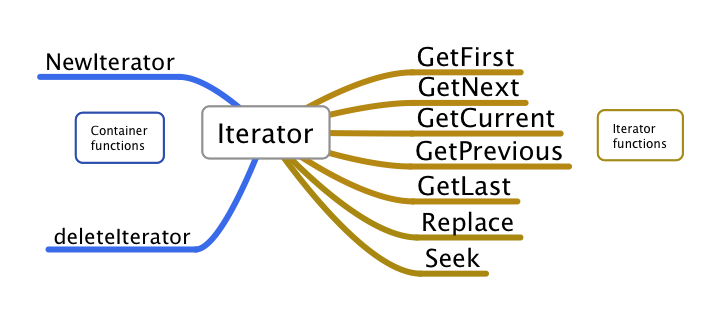
\includegraphics[scale=0.62]{Iterator.png}\par
The iterator object exposes at least the functions "GetFirst", for initializing the loop, and "GetNext", for getting the next element in the sequence. 
The functions "NewIterator" and "deleteIterator" are specific to each container interface even if they all have the same syntax.
\subsection{The interface}
\renewcommand{\container}{Iterator}
\begin{verbatim}
typedef struct _Iterator {
    void *(*GetNext)(Iterator *);
    void *(*GetPrevious)(Iterator *);
    void *(*GetFirst)(Iterator *);
    void *(*GetCurrent)(Iterator *);
    void *(*GetLast)(Iterator *);
    void *(*Seek)(Iterator *it,size_t pos);
    int (*Replace)(Iterator *it, void *data, int direction);
} Iterator;
\end{verbatim}
%--------------------------------------------------------------------------------------------------------------------------
\api{GetCurrent}
    void *(*GetCurrent)(Iterator *);
\end{verbatim}
\apidescription Returns the element at the cursor position.
\apierrors
\doerror{BADARG} The iterator pointer is \Null.
\returns
A pointer to the current element or \Null, if the container is empty or an error occurs. If the container is read-only, a pointer to a copy of the element is returned. This pointer is valid only until the next iterator function is called.
%--------------------------------------------------------------------------------------------------------------------------
\api{GetFirst}
    void *(*GetFirst)(Iterator *);
\end{verbatim}
\apidescription
This function initializes the given iterator to the first element in the container. For sequential operators this is the element with index zero. In 
associative operators which element is the first is implementation defined and can change if elements are added or removed from the container.

If the container is empty the result is \Null.
\apierrors
\doerror{BADARG} The iterator pointer is \Null.
\returns
A pointer to the first element or \Null, if the container is empty or an error occurs. If the container is read-only, a pointer to a copy of the element 
is returned. This pointer is valid only until the next iterator function is called.
\example
Iterator *myIterator;
List *myList;
myType *obj; // "myList" stores objects of type "myType"
myIterator = iList.NewIterator(myList); // Request iterator
for (obj = myIterator->GetFirst(myIterator); 
     obj != NULL; 
     obj = myIterator->GetNext(myIterator)) {
     //Use obj here
}
iList.deleteIterator(myIterator); // Reclaim memory
\end{verbatim}
%--------------------------------------------------------------------------------------------------------------------------

\api{GetNext}
    void *(*GetNext)(Iterator *);
\end{verbatim}
\apidescription
Positions de cursor at the next element and returns a pointer to its contents. If the iterator is at the end of the container the result is \Null 
and the iterator remains at the last position, a subsequent call to GetCurrent returns the last element.

If the container is read-only, a pointer to a copy of the object is returned. This pointer is valid only until the next iterator function is called.
\apierrors
\doerror{BADARG} The iterator pointer is \Null.
\doerror{OBJECT\_CHANGED} The container has been modified and the iterator is invalid. Further calls always return \Null.
\returns
A pointer to the next element or \Null, if the cursor reaches the last element. If the container is read-only, a pointer to a copy of the element is 
returned, valid until the next element is retrieved
%--------------------------------------------------------------------------------------------------------------------------
\api{GetPrevious}
    void *(*GetPrevious)(Iterator *);
\end{verbatim}
\apidescription
Positions de cursor at the previous element and returns a pointer to its contents. If the pointer is at the beginning of the container the
result is \Null and the iterator remains at the beginning, a subsequent call to GetCurrent will return the first element of the container.


This function is meaningful only in sequential containers. Its existence in associative containers is implementation defined. Even in sequential 
containers, it can be very expensive to find a previous element, for instance in single linked lists. In those cases it can always return \Null.

\apierrors
\doerror{BADARG} The iterator pointer is \Null.
\doerror{OBJECT\_CHANGED} The container has been modified and the iterator is invalid. Further calls always return \Null.
\returns
A pointer to the previous element or \Null, if the cursor reached the first element already. If the container is read-only, a pointer to a copy of the 
element is returned.
\example
Iterator *myIterator;
List *myList;
myType *obj; // "myList" stores objects of type "myType"
myIterator = iList.NewIterator(myList); // Request iterator
for (obj = myIterator->GetLast(myIterator); 
     obj != NULL; 
     obj = myIterator->GetPrevious(myIterator)) {
     //Use obj here
}
iList.deleteIterator(myIterator); // Reclaim memory
\end{verbatim}

%--------------------------------------------------------------------------------------------------------------------------
\api{GetLast}
    void *(*GetLast)(Iterator *);
\end{verbatim}
\apidescription
Positions the cursor at the last element and returns a pointer to it. Returns \Null if the container is empty.  If the container is read-only, a pointer 
to a copy of the element is returned.

This function is meaningful only in sequential containers. Its existence in associative containers is implementation defined. Even in sequential 
containers, it can be very expensive to find the last element, for instance in single linked lists. In those cases it can always return \Null.
\apierrors
\doerror{BADARG} The iterator pointer is \Null.
\doerror{OBJECT\_CHANGED} The container has been modified and the iterator is invalid. Further calls always return \Null.
%--------------------------------------------------------------------------------------------------------------------------
\api{Seek}
void *(*Seek)(Iterator *it,size_t pos);
\end{verbatim}
\apidescription
Positions the given iterator at the indicated position and then returns a pointer to the element's data at that position. 
If the position is bigger than the last element of the container, the last element position will be used.

This function is supported in sequential containers only.
\apierrors
\doerror{BADARG} The iterator pointer is \Null.
\doerror{OBJECT\_CHANGED} The container has been modified and the iterator is invalid. Further calls always return \Null.
\returns
A pointer to the data of the given element or \Null if an error occurs.
%--------------------------------------------------------------------------------------------------------------------------
\api{Replace}
int (*Replace)(Iterator *it,void *data, int direction);
\end{verbatim}
\apidescription
Replaces the current object pointed by the given iterator with the new data. If the\param{data} argument is \Null the element is erased from the
container. If the \param{direction} parameter is different from zero, in sequential containers the iterator will point to the next element,
otherwise it will point to the previous element. In associative containers this parameter is ignored and the iterator is always set to the next
element, if any.
\apierrors
\doerror{BADARG} The iterator pointer is \Null.
\doerror{OBJECT\_CHANGED} The container has been modified and the iterator is invalid. Further calls always return \Null.
\doerror{READONLY} The container is read only.
\returns A positive value if the element was changed or erased, zero if the container was empty, or a negative error code if an error occurred.

%--------------------------------------------------------------------------------------------------------------------------
%                    The observer interface
%--------------------------------------------------------------------------------------------------------------------------
\section{The observer interface}
\index{observer}
\renewcommand{\container}{Observer}
In its general form, the observer design pattern can be defined as a one-to-many dependency between objects so that when one object 
changes state, all its dependents are notified and updated automatically. 

When a container changes its state, specifically when elements are added or removed, it is sometimes necessary to update relationships that 
can be very complex.
The observer interface is designed to simplify this operation by allowing the container to emit \textsl{notifications} to other objects that have 
previously manifested interest in receiving them by \textsl{subscribing} to them. In general notifications are sent only when one of the defined
operations for a container occur, mostly operations that change the number of elements.

This interface then, establishes a relationship between two software entities:
\begin{enumerate}
\item The container, that is responsible for sending the notifications when appropriate
\item The receiver, that is an unspecified object represented by its callback function that is called when a change occurs that matches the
notifications specified in the subscription.
\end{enumerate}

Since this relationship needs both objects, it will be finished when either object goes out of scope or breaks the relationship for whatever 
reason. Both objects can unsubscribe (terminate) their relationship.
\subsection{Caveats}
\begin{itemize}
\item
It is in general a bad idea to modify the object being observed during a notification since this could trigger other notification
messages. Implementations are not required to avoid this situation that is the responsibility of the programmer. Contrary to the iterator interface
no error is issued when a possible infinite loop is started. Implementations may catch the error by limiting the number of recursive
invocations of this interface but they are not required to do so.
\item
Since all messages sent by the containers have different type of information in the same two arguments that each message is associated with,
there is no possible compile time control of the usage of the received pointers or numbers. The observer function must correctly 
discriminate between the different messages it can receive\footnote{An alternative design would have been to specify not one type of
observer function but to define a different function type for each possible message the containers could send. We would have then a SubscribeAdd
SubscribeErase SubscribeReplace functions, combined with NotifyAdd, NotifyErase, NotifyReplace functions. That design would have been easier to
control at compile time. It was rejected because of the increased complexity of the interface and the necessity for the user to define a lot
of functions just to know when something as simple as "Was this container modified?" happened.

Obviously implementations can add that type of interface if they wish. In future revisions of this specifications this question will be posed again, with more actual use data to make more informed decisions.}.
\end{itemize}

\subsection{The interface}
\begin{verbatim}
typedef void (*ObserverFunction)(const void *ObservedObject,
                                 unsigned Operation, 
                                 void *ExtraInfo[]);

typedef struct tagObserverInterface {
    int (*Subscribe)(void *ObservedObject, 
                     ObserverFunction callback, unsigned Operations);
    int (*Notify)(const void *ObservedObject,unsigned operation,
                  void *ExtraInfo1,void *ExtraInfo2);
    size_t (*Unsubscribe)(void *ObservedObject,
                          ObserverFunction callback);
} ObserverInterface;
extern ObserverInterface iObserver;
\end{verbatim}
\api{ObserverFunction}
typedef void (*ObserverFunction)(void *ObservedObject,
                                 unsigned Operation, void *ExtraInfo[]);
\end{verbatim}
\apidescription
This function will be called by the interface when a notification is received for an observed object.  The call happens after all arguments have been processed, the actual work of the function is finished (when adding an object) or not yet done (when destroying an object). 
The container is in a consistent state. For the callbacks that are called when an object is deleted from a
container the call happens before any call to \texttt{free()} and before any call to a destructor (if any) is done. For the calls that add an object
the callback is called after the container has been modified. 

Arguments:
\begin{enumerate}
\item \texttt{ObservedObject}: Specifies the object that sends the notification, i.e. the container
that has the subscription. It is assumed that this container conforms to the \texttt{iGeneric} interface.
\item \texttt{Operation}: The operation that provoked the notification. Since it is possible to subscribe to several operations with only one callback function,
this argument allows the callback to discriminate between the operation notifications.
\item \texttt{ExtraInfo}: This argument is specific to each operation and conveys further information\footnote{See the full list and the description of all notifications at the end of this section} for each operation.
\end{enumerate}

None of the arguments will be ever \Null or zero.
\api{Subscribe}
int (*Subscribe)(void *ObservedObject, ObserverFunction callback, 
                 unsigned Operations);
\end{verbatim}
\apidescription
This function establishes the relationship between the observed object (argument 1) and the observer, represented by its callback (argument 2).
The third argument establishes which operations are to be observed.
This operation performs an allocation to register the relationship in the observer interface tables, therefore it can fail with an out of memory 
condition.
\apierrors
\doerror{BADARG} The observed object pointer is \Null, the callback function pointer is \Null, or the operations argument is zero.
\doerror{NOMEMORY} There is not enough memory to proceed.
\returns An integer greater than zero if the relationship was established, a negative error code otherwise.

\api{Notify}
int (*Notify)(void *ObservedObject,unsigned Operation,
                  void *ExtraInfo1,void *ExtraInfo2);
\end{verbatim}
\apidescription
This function will be used by the container to send a message to the receiver callback. The arguments correspond roughly to the arguments the callback
function will receive. "Notify" will call all the objects that are observing \texttt{ObservedObject} and that have subscribed to one of the 
operations
specified in the \texttt{Operation} argument. This implies a search through the observer interface table, and possibly several calls, making
this function quite expensive. The time needed is roughly proportional to the number of registered callbacks and the complexity of the callbacks
themselves.
\apierrors
\doerror{BADARG} The ObservedObject pointer is \Null or the Operation argument is zero.
\returns A positive number with the number of objects that received the notifications, zero if there was no match for the combination of observed object and operations specified, or a negative error code.


\api{Unsubscribe}
size_t (*Unsubscribe)(void *ObservedObject, ObserverFunction callback);
\end{verbatim}
\apidescription
This function breaks the relationship between the observed object and the observer. There are several combinations of both arguments:
\begin{itemize}
\item The \texttt{ObservedObject} argument is \Null. This means that the \texttt{callback} object wants to break its relationship to all objects it is
observing. The observer interface will remove all relationships that contain this callback from its tables.
\item The \texttt{callback} argument is \Null. This means that the given \texttt{ObservedObject} is going out of scope and wants to break all
relationships to all its observers. The interface removes from its tables all relationships that have this object as the observed object.
This happens normally immediately after the notification \texttt{FINALIZE} is sent.
\item If both \texttt{callback} and \texttt{ObservedObject} are non \Null, only the matching relationship will be removed from the tables.
\end{itemize}
\subsection{Notification messages}
\begin{longtable}{p{2.5cm}|p{5cm}|p{4.5cm}}
{\textbf{Operation}} &
{\textbf{Argument 1}} &
{\textbf{Argument 2}}\\
\hline
\endfirsthead

%This is the header for the remaining page(s) of the table...

\multicolumn{3}{c}{{\tablename} \thetable{} -- Continued} \\[0.5ex]
%\hline \hline
{\textbf{Operation}} &
{\textbf{Argument 1}} &
{\textbf{Argument 2}}\\
\hline
\endhead
Add&Pointer to the new object& \Null or slice specs if any\\ \hline
AddRange&A \texttt{size\_t} with the number of objects added&Pointer to a table of \textsl{n} elements that were added\\ \hline
Append&A pointer to the object being appended. It is of the same type as the object emitting the notification&  \Null\\ \hline
Clear&Pointer to the container being cleared& \Null\\ \hline
Copy&Pointer to the copy of the container& \Null\\ \hline
Erase&Pointer to the object being deleted. The object is still valid& \Null\\ \hline
EraseAt&Pointer to object being deleted&Position (as size\_t)\\ \hline
Finalize& \Null& \Null\\ \hline
Insert&Pointer to the new object being inserted&A \texttt{size\_t} with the position of the object being inserted if applicable\\ \hline
InsertIn&Pointer to the object being inserted, that has the same type as the object sending the notification& \Null\\ \hline
Pop&Pointer to the object being popped& \Null\\ \hline
Push&Pointer to the object being pushed& \Null\\ \hline
ReplaceAt&Pointer to the old value&Pointer to the new value\\ \hline

\end{longtable}
Here is a complete example that demonstrates some of the above functions.
\example
include "containers.h"
static void fn(void *ObservedObject, unsigned operation,
               void *extraInfo[])
{
    printf("Object is %p, operation is %d\n",ObservedObject,operation);
}
int main(void)
{
    ValArrayInt * vInt = iValArrayInt.CreateSequence(24,0,1);

    printf("Original array: \n");
    iValArrayInt.Fprintf(vInt,stdout,"%d ");
    iObserver.Subscribe(vInt,fn,CCL_ADD|CCL_FINALIZE);
    printf("Adding an integer\n");
    iValArrayInt.Add(vInt,4096);
    iValArrayInt.Fprintf(vInt,stdout,"%d ");
    iValArrayInt.Finalize(vInt);
}
OUTPUT:
Original array: 
0 1 2 3 4 5 6 7 8 9 10 11 12 13 14 15 16 17 18 19 20 21 22 23 
Adding an integer
Object is 0x100100080, operation is 1
0 1 2 3 4 5 6 7 8 9 10 11 12 13 14 15 16 17 18 19 20 21 22 23 4096 
Object is 0x100100080, operation is 16
\end{verbatim}
We setup our observer function calling the Subscribe API. We request to be notified when there is an addition and when the object
finalizes. Our callback function does nothing but print some of its arguments. We see that we get called when the requested operations are performed.
\section{Types used by the library}
Here is a complete list of all the auxiliary data types defined by the library. This definitions are the minimum requirements, i.e. all the fields mentioned here must be present in all implementations. Many implementations will need more fields, that in all cases can be added to the data
types present here without affecting conformance. 

The order and specific layout of the structure fields are not normative: an implementation can change this order, or insert extra fields between them.
If an implementation does insert fields between the here mentioned fields it becomes binary incompatible with the sample implementation and maybe
with other implementations that respect this order. An alternative way to expand the structure is to add fields at the end, retaining binary
compatibility with other implementations. This choice is obviously implementation defined.

An implementation can change the signature of the function pointers described here by adding optional arguments after the required ones using the
standard C mechanism for variable arguments functions. This retains source and binary compatibility with the standard, allowing for extensions
specific to the implementation.
\subsection{CompareInfo}
\begin{verbatim}
typedef struct tagCompareInfo {
    void *ExtraArgs;
    const void *ContainerLeft;
    const void *ContainerRight;
} CompareInfo;
\end{verbatim}
This structure will be passed to the comparison functions. The \verb,ExtraArgs, pointer will receive the pointer that was passed to the calling function. If both elements being compared are members of a single container, the \texttt{ContainerRight} member will be \Null and \verb,ContainerLeft,
will hold a pointer to the container where both elements belong. Otherwise \verb,ContainerLeft, will hold a pointer to the container that holds
the first argument, and \verb,ContainerRight, to the one that holds the second. 

\subsection{CompareFunction}
\index{CompareFunction}
\begin{verbatim}
typedef int (*CompareFunction)(const void *elem1, 
                               const void *elem2, 
                               CompareInfo *ExtraArgs);
\end{verbatim}
This type defines the function used to compare two elements.
The result should be less than zero if elem1 is less than elem2, zero if they are equal, and bigger than zero if elem1 is bigger than element 2.

The default comparison function is \texttt{memcmp}. This function will compare all the object's area, including eventually padding bytes added by
compilers for alignment reasons. To minimize this problem always zero the objects before assigning the values. For instance:
\begin{verbatim}
struct Data {
    int Age; // Here the compiler can introduce padding bytes
    double Weight;
};

int fn(void)
{
    struct Data m;
    memset(&m,0,sizeof(m));
    m.Age = 23;
    m.Weight = 76;
    iVector.Add(DataCollection,&m);
}
\end{verbatim}
By zeroing the structure before making the assignments, we have a known value in the padding bytes. If we make comparisons with memcmp, they will
work correctly.

Obviously the best way to avoid this problem is to avoid any default comparison function by defining one.

\subsection{Save function}
\index{SaveFunction}
\begin{verbatim}
typedef int (*SaveFunction)(const void *element, 
                               void *ExtraArg, 
                               FILE *OutputStream);
\end{verbatim}
This function should save the given element into the given stream.  The \verb,ExtraArg, argument receives any argument passed to the Save function.
The result should be bigger than zero if the operation completed successfully, zero or less than zero otherwise.

What the save function does is unknown to the rest of the library, basically the only requirement is that its output should be understood by the
read function, when called to read each element. The size of the written data can be bigger (or smaller) than the size of each stored element,
according to the specific requirements of the application data. This allows to write save functions that would write a complete data set, including
embedded objects into the stream. For instance a save function can save the contents pointed by a character pointer instead of the pointer value 
that would be meaningless when read again.

The default save function provided by the implementation just writes the contents of each element into the stream. Embedded pointers aren't followed.
\subsection{Read function}
\index{ReadFunction}
\begin{verbatim}
typedef int (*ReadFunction)(void *element, 
                               void *ExtraArg, 
                               FILE *InputStream);
\end{verbatim}
This function should read into the given element from the given stream. The \verb,ExtraArg, argument is passed to the container read function and allows to pass an argument to the user defined save function. The amount of data read is unknown to the rest of the software and the only requirement
is that it should reverse the work of the save function.

The default read function provided by the implementation should read the contents of one element from the stream and add it to the result container.

The result is bigger than zero if the operation completed successfully, zero or less than zero otherwise.
\subsection{Error function}
\index{ErrorFunction}
\begin{verbatim}
typedef void *(*ErrorFunction)(const char *functionName,int code,...);
\end{verbatim}
This function type is used to handle errors in each container. The first argument is the name of the function where the error occurred, the second is a 
negative error code. No checks are performed on the function name argument, and other information or messages could be included in the message.

Note that this function is roughly compatible with the prototype of snprintf, and could be used with a format string, a buffer size, and a series of 
arguments corresponding to the arguments the format requires. The only problem is the conversion between \verb,int, and \verb,size_t,.

The result value of the default error function is always \Null. This result will be in most cases ignored, except in the vector container where
it can be used to return special values in the case of the \verb,INDEX, error.

When \verb,iVector, interface detects an index error, it will pass in the extra arguments the array pointer and a \verb,size_t, containing 
the out of bounds index.
\subsection{Destructor function}
\index{DestructorFunction}
\begin{verbatim}
typedef int (*DestructorFunction)(void *object);
\end{verbatim}
This function is called when an object is being destroyed. An object is destroyed when:
\begin{itemize}
\item An \texttt{Erase} call is done.
\item A \texttt{Replace} call is done.
\item The \texttt{Clear} call is done.
\item The \texttt{Select} call is done with some element of the mask to zero.
\item The \texttt{Resize} function is called with an argument less than the size of the container.
\end{itemize}
This function should free any memory used by pointers within the object \textbf{without} freeing the object memory itself. In most cases the memory
used by the library is \textbf{not} allocated with malloc. Its result type is less than zero when an error occurred or greater than zero when
it finished successfully. It is implementation defined what happens if a destructor encounters an error.

%--------------------------------------------------------------------------------------------------------------------------
%                                                   LISTS
%--------------------------------------------------------------------------------------------------------------------------
\chapter{The containers}
\index{List}
\renewcommand{\container}{List}
\section{The List interfaces: iList, iDlist}
The list container appears in two flavors: 
\begin{itemize}
\item
single linked lists: the iList type
\item
double linked lists the iDlist type
\end{itemize}
The space overhead of single linked lists is smaller at the expense of more difficult access to the elements. It is up to the application programmer to decide which container fits best in his/her application
\footnote{
The single linked list container corresponds to the C++ STL \texttt{forward\_list}.
}.

It is often more efficient to get the next element from a list starting with the previous element instead of searching the whole list starting from the beginning. For this, the list and the Dlist containers provide:
\begin{ShorterItemize}
\item \verb,FirstElement, Start of the list
\item \verb,LastElement, End of the list
\item \verb,NextElement, Returns a pointer to the next element
\item \verb,PreviousElement, Only in double linked lists. Returns a pointer to the previous element.
\item \verb,ElementData, Extracts a pointer to the element data 
\item \verb,SetElementData, Modifies one element of the list.
\item \verb,Advance, Returns the data of an element and advances the given pointer in one operation.
\item \verb,MoveBack, Returns the data of an element and moves back the pointer one element. This operation is available only in double linked lists.
\end{ShorterItemize}

These operations can't be done in a read-only list.

The exact layout of the \verb,ListElement, structure is undefined and private to each implementation. This is the reason for providing the \verb,ElementData, function: it hides the exact position and layout of the data from user code, that remains independent from implementation details.

The interfaces of both containers are very similar. Double linked lists support all functions in single linked ones, and add a few more. To avoid unnecessary repetition we document here all the single linked list interface, then only the functions that the Dlist interface adds to it.
\index{iList}\index{lists!single linked}
\begin{verbatim}
typedef struct tagListInterface {
   int (*Add)(List *L,const void *newval);
   int (*AddRange)(List *L, size_t n,const void *data);
   void *(*Advance)(ListElement **pListElement);
   int (*Append)(List *l1,List *l2);
   int (*Apply)(List *L,int(Applyfn)(void *,void *),void *arg);
   void *(*Back)(const List *l);
   int (*Clear)(List *L);
   int (*Contains)(const List *L,const void *element);
   List *(*Copy)(const List *L);
   int (*CopyElement)(const List *list,size_t idx,void *OutBuffer);
   List *(*Create)(size_t element_size);
   List *(*CreateWithAllocator)(size_t elementsize,
         const ContainerAllocator *mm);
   void *(*ElementData)(ListElement *le);
   int (*Equal)(const List *l1,const List *l2);
   int (*Erase)(List *L,const void *);
   int (*EraseAll)(List *l,const void *);
   int (*EraseAt)(List *L,size_t idx);
   int (*EraseRange)(List *L,size_t start,size_t end);
   int (*Finalize)(List *L);
   ListElement *(*FirstElement)(List *l);
   void *(*Front)(const List *l);
   const ContainerAllocator *(*GetAllocator)(const List *list);
   void *(*GetElement)(const List *L,size_t idx);
   size_t (*GetElementSize)(const List *l);
   unsigned (*GetFlags)(const List *L);
   ContainerHeap *(*GetHeap)(const List *l);
   List *(*GetRange)(const List *l,size_t start,size_t end);
   int (*IndexOf)(const List *L,const void *SearchedElement,
        void *ExtraArgs,size_t *result);
   List *(*Init)(List *aList,size_t element_size);
   int (*InitIterator)(List *L,void *buf);
   List *(*InitWithAllocator)(List *aList,size_t element_size,
         const ContainerAllocator *mm);
   List *(*InitializeWith)(size_t elementSize,size_t n,
         const void *data);
   int (*InsertAt)(List *L,size_t idx,const void *newval);
   int (*InsertIn)(List *l, size_t idx,List *newData);
   ListElement *(*LastElement)(List *l);
   List *(*Load)(FILE *stream, ReadFunction loadFn,void *arg);
   Iterator *(*NewIterator)(List *L);
   ListElement *(*NextElement)(ListElement *le);
   int (*PopFront)(List *L,void *result);
   int (*PushFront)(List *L,const void *str);
   int (*RemoveRange)(List *l,size_t start, size_t end);
   int (*ReplaceAt)(List *L,size_t idx,const void *newval);
   int (*Reverse)(List *l);
   int (*RotateLeft)(List *l, size_t n);
   int (*RotateRight)(List *l,size_t n);
   int (*Save)(const List *L,FILE *stream, SaveFunction saveFn,
        void *arg);
   int (*Select)(List *src,const Mask *m);
   List *(*SelectCopy)(const List *src,const Mask *m);
   CompareFunction (*SetCompareFunction)(List *l,CompareFunction fn);
   DestructorFunction (*SetDestructor)(List *v,DestructorFunction fn);
   int (*SetElementData)(List *l, ListElement *le,void *data);
   ErrorFunction (*SetErrorFunction)(List *L,ErrorFunction);
   unsigned (*SetFlags)(List *L,unsigned flags);
   size_t (*Size)(const List *L);
   size_t (*Sizeof)(const List *l);
   size_t (*SizeofIterator)(const List *);
   ListElement *(*Skip)(ListElement *l,size_t n);
   int (*Sort)(List *l);
   List *(*SplitAfter)(List *l, ListElement *pt);
   int (*UseHeap)(List *L, const ContainerAllocator *m);
   int (*deleteIterator)(Iterator *);
} ListInterface;
\end{verbatim}

\par\noindent
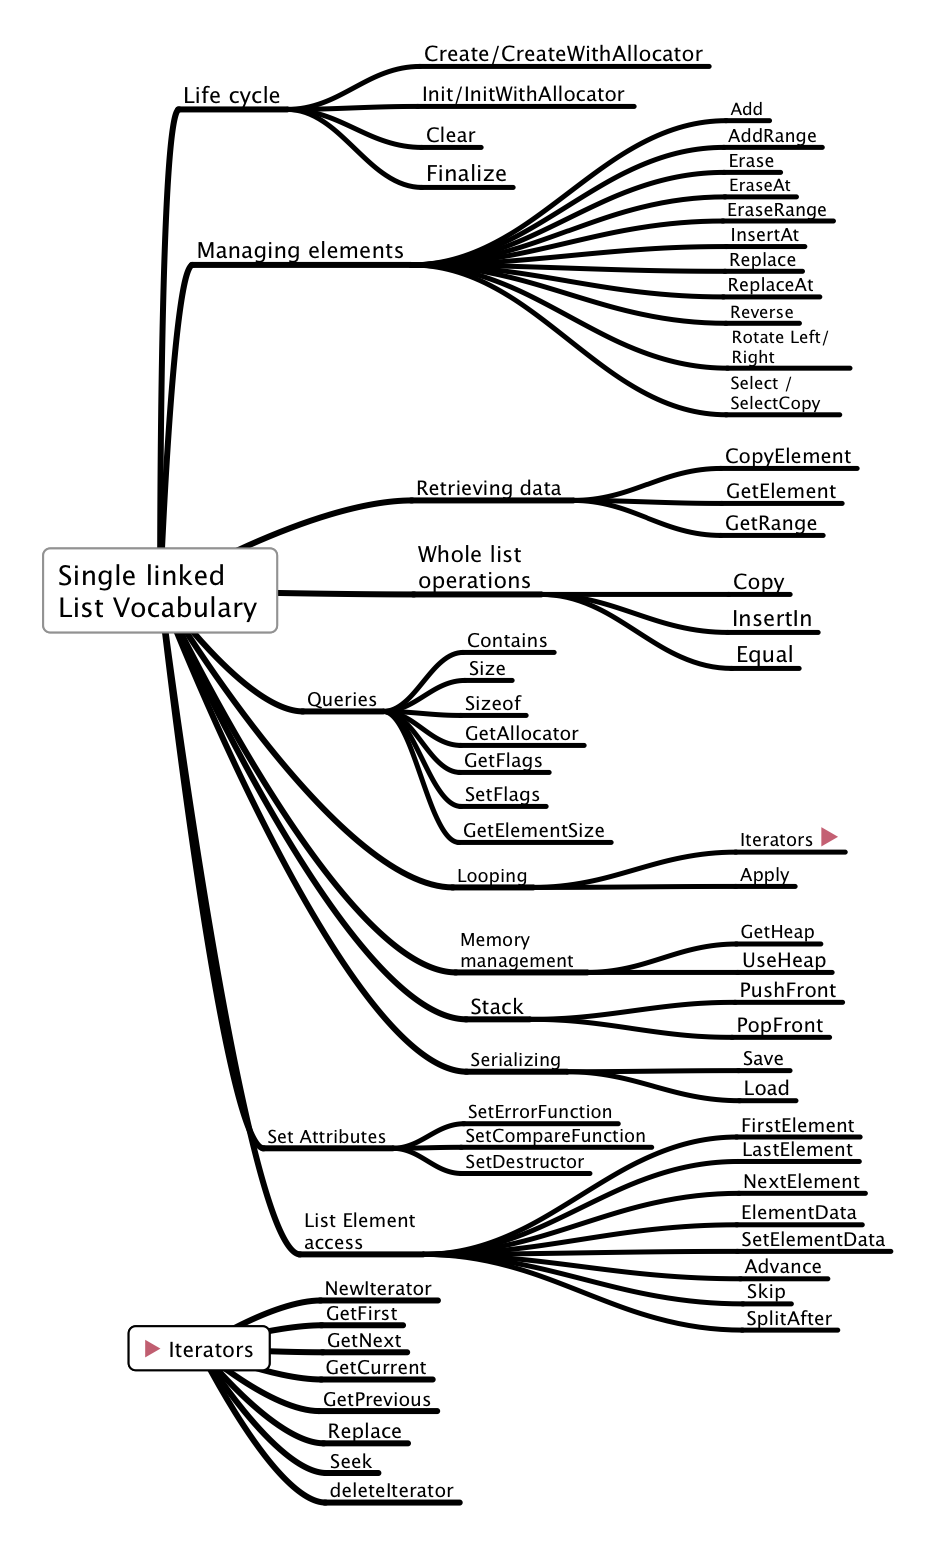
\includegraphics[scale=0.45]{ListVocabulary.png}
\subsection{General remarks}
Lists are containers that store each element in a sequence, unidirectionally (single linked lists) or bidirectionally (double linked lists).
The advantage of linked lists is their flexibility. You can easily and with a very low cost remove or add elements by manipulating the links between the elements. Single linked lists have less overhead than their double linked counterparts (one pointer less in each node), but they tend to use a lot of computer power when inserting elements near the end of the list: you have to follow all links from the beginning until you find the right one.

The list nodes themselves do not move around, only their links are changed. This can be important if you maintain pointers to those elements. Obviously, if you delete a node, its contents (that do not move) could be recycled to contain something else than what you expect.

The iList interface consists (as all other interfaces) of a table of function pointers. The interface describes the behavior of the List container.

The stack operations push and pop are provided with PushFront and PopFront because they have a very low cost, insertion at the start of a single linked list is very fast. PushBack is the equivalent of the \verb,Add, operation, but PopBack would have a very high cost since it would need going through all the list. 

The list container features in some implementations a per list error function.  This is the function that will be called for any errors, except in  
cases where no list object exists: the creation function, or the error of getting a \Null pointer instead of a list pointer. In those cases the general 
iError interface is used, and iError.RaiseError is called. The default value of the list error function is the function iError.RaiseError at the moment 
the list is created.

Other implementations of this interface may specialize list for a certain category of uses: lists of a few elements would try to reduce overhead by 
eliminating a per list error function and replace it with the standard error function in iError, for instance, eliminating their fields in the header. 
If the read-only flag support is dropped, the whole "Flags" field can be eliminated. In such an implementation, the SetFlags primitive would always 
return an error code.

The sample implementation of the list container supports the following state flags:
\begin{verbatim}
#define CONTAINER_READONLY          1
\end{verbatim}
If this flag is set, no modifications to the container are allowed, and the Clear and Finalize functions will not work. Only copies of the data are 
handed out, no direct pointers to the data are available.
\begin{verbatim}
#define CONTAINER_SORTED_FRONT      2
#define CONTAINER_SORTED_BACK       4
\end{verbatim}
If this flag is set, the container is maintained always in sorted order, with the biggest element at the index zero for \verb,CONTAINER_SORTED_FRONT,
or with the biggest element at the end if \verb,CONTAINER_SORTED_BACK, is set. It is an error if both flags are set, and the results in that  case
are implementation defined.
\subsubsection{Specializations}
All "specialized" containers share the same interface with the following exceptions:
\begin{ShorterItemize}
\item The functions where a \verb,void *, to the element data is passed or where a \verb,void *, is the result of the operation are replaced with the 
actual data type of the specialization. For instance the \verb,GetElement, API instead of returning a void pointer returns a pointer to the specific 
data type: an 
integer for \verb,intList,, a double for \verb,doubleList, etc.
\item The creation and initialization functions that construct a new container receive one argument less than its generic counterparts since the
size of each element is fixed.

To make things clear and to save work from the library user some specializations are delivered with the sample implementation to show how a
\textsl{file templated} container looks like.
\end{ShorterItemize}
\begin{center}
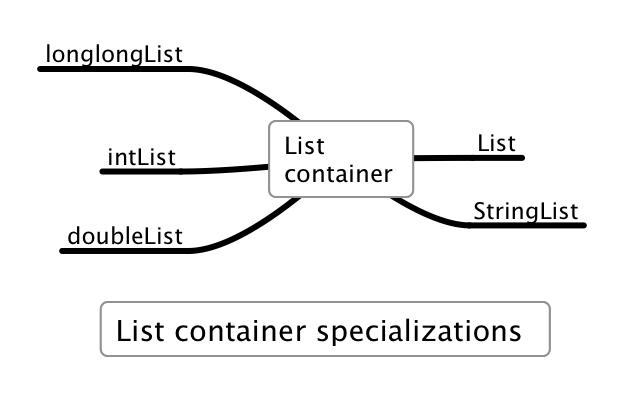
\includegraphics[scale=0.625]{ListContainerSpecializations.png}
\end{center}
In the right side of the drawing we see the generic list container using generic pointers (\verb,void *,) and the stringlist container. Strings are 
special because in C their length is the result of a function call instead of being fixed like other data types.

In the left side, we see three specialized containers for some numeric data types. Those containers are generated using two types of source files:
\begin{ShorterItemize}
\item Parameter files: They define the data type and some other parameters like the comparison expression.
\item Templated files: They implement the specialized container. The pre-processor does the editing work on the templated file to yield several 
different type definitions. Using this interface has the advantage of ensuring compile time checking of the arguments to the API, what is not
possible using generic pointers.
\end{ShorterItemize}

%--------------------------------------------------------------------------------------------------------------------------
\api{Add}
int (*Add)(List *l,const void *data);
int (*Add)(TYPEList *l, TYPE data);
\end{verbatim}

\apidescription
Adds the given element to the container. In its generic form it is assumed that "data" points to a contiguous memory area of at least ElementSize 
bytes. Inits specialized form the data is passed by value. Returns a value greater than zero if the addition of the element to the list completed 
successfully, a negative error code otherwise.

\apierrors
\doerror{BADARG} The list or the data pointers are \Null.
\doerror{READONLY} The list is read-only. No modifications allowed.
\doerror{NOMEMORY} Not enough memory to complete the operation.
\Const The input data is not modified.
\returns
A positive number if the element was added or a negative error code otherwise.
\example
/* This example shows how to: 
(1) Create a linked list of "double" data
(2) Fill it using the "Add" function
(3) Print it using the GetElement function */
#include <containers.h>
static void PrintList(List *AL)
{
    size_t i;
    for (i=0; i<iList.Size(AL);i++) {
        printf("%g ",*(double *)iList.GetElement(AL,i));
    }
    printf("\n");
}
static void FillList(List * AL,size_t siz)
{
    size_t i;

    for (i=0; i<siz;i++) {
        double d = i;
        iList.Add(AL,&d);
    }
}

int main(void)
{
    List *AL = iList.Create(sizeof(double));
    FillList(AL,10);
    PrintList(AL);
    return 0;
}
OUTPUT:
0 1 2 3 4 5 6 7 8 9
\end{verbatim}
Using the templated container implementation:
\begin{verbatim}
#include <containers.h>
#include <doublelist.h>
static void PrintList(doubleList *AL)
{
    size_t i;
    for (i=0; i<idoubleList.Size(AL);i++) {
        printf("%g ",idoubleList.GetElement(AL,i));
    }
    printf("\n");
}
static void FillList(doubleList * AL,size_t siz)
{
    size_t i;

    for (i=0; i<siz;i++) {
        idoubleList.Add(AL,(double)i);
    }
}

int main(void)
{
    doubleList *AL = idoubleList.Create();
    FillList(AL,10);
    PrintList(AL);
    return 0;
}
OUTPUT:
0 1 2 3 4 5 6 7 8 9
\end{verbatim}

%--------------------------------------------------------------------------------------------------------------------------
\api{Advance}
void *(*Advance)(ListElement **ppElement);
TYPE *(*Advance)(TYPEListElement **ppElement);
\end{verbatim}
\apidescription
Given the address of a pointer to an element, it returns a pointer to the data stored into that element and writes the address of the next element
into its argument \verb,ppElement,. If ppElement is\Null it returns\Null. If \verb,*ppElement, is\Null it also returns\Null, and obviously there 
is no advancing done.
\returns A pointer to the data stored in the given element or\Null if the data can't be retrieved.
%--------------------------------------------------------------------------------------------------------------------------
\api{AddRange}
    int (*AddRange)(List * AL,size_t n, void *data);
    int (*AddRange)(TYPEList * AL,size_t n, TYPE *data);
\end{verbatim}
\apidescription
Adds the n given elements to the end of the container. It is the same operations as the PushBack operation. It is assumed that "data" points to a 
contiguous memory area of at least n*ElementSize bytes. If \textsl{n} is zero no error is issued even if the array pointer or the data pointer are 
\Null.
\apierrors
\doerror{BADARG} The list or the data pointers are \Null, and n is not zero.
\doerror{READONLY} The list is read-only. No modifications allowed.
\doerror{NOMEMORY} Not enough memory to complete the operation.
\returns
A positive number if the operation completed, negative error code otherwise.

%--------------------------------------------------------------------------------------------------------------------------
\api{Append}
    int (*Append)(List *list1,List *list2);
\end{verbatim}
\apidescription
Appends the contents of list2 to list1 and destroys list2.
\apierrors
\doerror{BADARG} Either list1 or list2 are \Null.
\doerror{READONLY} One or both lists are read only.
\doerror{INCOMPATIBLE} The size of the elements in the lists differ, or the lists allocators are different \footnote{Since the allocator's free() 
function will be used by the finalize function to free the memory used by the list, it is imperative that both lists share the same allocator. \par
Some implementations could make a copy of the second list using the first list allocator, then append, then release all the storage but that would
change significantly the execution time. It is better to return an error in this case.}. 
\returns
A positive value if the operation succeeded, or a negative error code otherwise.
\example
#include <containers.h>
static void PrintList(List *AL)
{
    size_t i;
    for (i=0; i<iList.Size(AL);i++) {
        printf("%g ",*(double *)iList.GetElement(AL,i));
    }
    printf("\n");
}
static void FillList(List * AL,size_t siz)
{
    size_t i;

    for (i=0; i<siz;i++) { double d = i; iList.Add(AL,&d);}
}

int main(void)
{
    List *L1 = iList.Create(sizeof(double));
    List *L2 = iList.Create(sizeof(double));
    FillList(L1,10);
    FillList(L2,10);
    iList.Append(L1,L2);
    PrintList(L1);
    return 0;
}
OUTPUT:
0 1 2 3 4 5 6 7 8 9 0 1 2 3 4 5 6 7 8 9
\end{verbatim}
%--------------------------------------------------------------------------------------------------------------------------
\api{Apply}
    int (*Apply)(List l,int (Applyfn)(void *,void *),void *arg);
    int (*Apply)(List l,int (Applyfn)(TYPE ,void *),void *arg);
\end{verbatim}
\apidescription
Will call the given function for each element of the list. The first argument of the callback function receives an element of the list. The second argument of the callback is the arg argument that the Apply function receives and passes to  the callback. This way some context can be passed to the callback, and from one element to the next.
Note that the result of the callback is not used. This allows all kinds of result types to be accepted after a suitable cast.
If the list is read-only, a copy of the element will be passed to the callback function.
\apierrors
\doerror{BADARG} Either list or Applyfn are \Null.
\doerror{NOMEMORY}: The list is read-only and there is no more memory to allocate the buffer to copy each element.
\notes
The list container of C++ has no direct equivalent, but in the algorithm part of the STL there is a "for\_each" construct, that does essentially the same. Java and C\# offer a similar "ForEach" functionality.
 
\example
#include <containers.h>
static int Callback(void *pElement,void *pResult)
{
    double *p = pElement;
    double *result = pResult;
    *result += *p;
    return 1;
}
    
void main(void) 
{
    double sum = 0;
    List *list = iList.Create(sizeof(double));
    double d = 2;
    iList.Add(list,&d);
    d = 3;
    iList.Add(list,&d);
    iList.Apply(list,Callback,&sum);
    // Here sum should be 5.
    printf("%g\n",sum);
}

/* Template file example */
#include <containers.h>
#include "doublelist.h"
static int Callback(double Element,void *pResult)
{
    double *result = pResult;
    *result += Element;
    return 1;
}
    
void main(void) 
{
    double sum = 0;
    doubleList *list = idoubleList.Create();
    iList.Add(list,2);
    iList.Add(list,3);
    iList.Apply(list,Callback,&sum);
    // Here sum should be 5.
    printf("%g\n",sum);
}
\end{verbatim}
The above example shows a function callback as used by "Apply". It receives two pointers, one to the current element and another to an extra argument that in this case contains a pointer to the sum. For each call to the callback, the function adds the contents of the element to the sum.

The main function creates a list, adds two elements with the values 2 and 3, and then calls "Apply" to get their sum using the callback.
%--------------------------------------------------------------------------------------------------------------------------
\api{Back}
const void *(*Back)(const List *list);
const TYPE  (*Back)(const TYPEList *l);
\end{verbatim}
\apidescription
Returns the last element of the given list or \Null if the list is empty.
\apierrors
\doerror{BADARG} The list pointer is \Null.
\doerror{READONLY} The list is read only.
\Const The input list is not modified.
\returns
The last element or \Null if the list is empty or an error occurs.
%--------------------------------------------------------------------------------------------------------------------------
\api{Clear}
    int (*Clear)(List *l);
\end{verbatim}
\apidescription
Erases all stored data and releases the memory associated with it. The list header will not be destroyed, and its contents will be the same as when the list was initially created. It is an error to use this function when there are still active iterators for the container.\footnote{Java, C++ and C\# have a similar "Clear" functionality.}
\apierrors
\doerror{BADARG} The list pointer is \Null.
\doerror{READONLY} The list is read only.
\returns
The result is greater than zero if successful, or an error code if an error occurs. 

\example
    List *l;
    int m = iList.Clear(l);
\end{verbatim}
%--------------------------------------------------------------------------------------------------------------------------
\api{Contains}
    int (*Contains)(List *list,void *data);
    int (*Contains)(TYPEList *l, TYPE data);
\end{verbatim}
\apidescription
Returns one if the given data is stored in the list, zero otherwise. The "data" argument is supposed to point to an element at least ElementSize bytes. The list's comparison function is used for determining if two elements are equal. This comparison function defaults to memcmp.
\apierrors
\doerror{BADARG} Either list or data are \Null.
\notes
C++ has std::find that does essentially the same . Java and C\# have a "Contains" method.
\example
    List *list;
    int r = iList.Contains(list,&data);
\end{verbatim}

%--------------------------------------------------------------------------------------------------------------------------
\api{Copy}
    List *(*Copy)(const List *L);
\end{verbatim}
\apidescription
A shallow copy of the given list is performed. Only ElementSize bytes will be copied for each element. If the element contains pointers, only the pointers are copied, not the objects they point to. The new memory will be allocated using the given list's allocator.
\apierrors
\doerror{NOMEMORY} There is not enough memory to complete the operation.
\doerror{BADARG} The given list pointer is \Null.
\Const The input list is not modified.
\notes
C++ has no direct equivalent but the assignment operator should work, Java and C\# support a copy method.
\example
    List *newList,*OldList;
    newList = iList.Copy(OldList);
    if (newList == NULL) { /* Error handling */ }
\end{verbatim}

%--------------------------------------------------------------------------------------------------------------------------
\api{CopyElement}
    int (*CopyElement)(const List *list,size_t idx,void *outBuffer);
    int (*CopyElement)(const TYPEList *list,size_t idx,TYPE *outBuffer);
\end{verbatim}
\apidescription
Copies the element data at the given position into the given buffer, assuming that at least ElementSize bytes of storage are available at the position pointed by the output buffer. The main usage of this function is to access data in a read only container for later modification.
\apierrors
\doerror{BADARG} The given list pointer or the output buffer are \Null.
\doerror{INDEX} The given position is out of bounds.
\Const The input list is not modified.
\returns
A positive value if the operation succeeded, or a negative error code if it failed.

\notes
Neither C\# nor Java provide this functionality because the treatment of pointers in those languages makes the need for such a construct unnecessary.

\example
    List *list; double d;
    if (iList.CopyElement(list,3,&d) > 0)
        printf("The value at position 3 is %g\n",d);
\end{verbatim}

%--------------------------------------------------------------------------------------------------------------------------
\api{Create}
    List *(*Create)(size_t element_size);
    TYPEList *(*Create)(void); // Template version
\end{verbatim}
\apidescription
The creation function returns an empty List container, initialized with all the default values.
The current memory manager is used to allocate the space needed for the List header. The list is supposed to contain elements of the same size. If the elements you want to store are of different size, use a pointer to them, and create the list with sizeof(void *) as the size parameter.
\returns
A pointer to a newly created List or \Null if an error occurs.
\apierrors
\doerror{NOMEMORY} There is not enough memory to complete the operation.
\doerror{BADARG} The given element size is zero or greater than what the implementation allows for maximum object size.

Errors provoke the call of the current default error function of the library since this is the creation function and there isn't a container specific error function yet.
\example
    List *ListOfDoubles = iList.Create(sizeof(double));
    doubleList *ListOfDoubles = idoubleList.Create();
\end{verbatim}
\api{CreateWithAllocator}
List *(*CreateWithAllocator)(size_t elem_size,
                             ContainerAllocator *allocator);
// Template file version
TYPEList *(*CreateWithAllocator)(ContainerAllocator *allocator);
\end{verbatim}
\apidescription
The creation function returns an empty List container, initialized with all the default values.
The given memory manager is used to allocate the space needed for the List header. The list is supposed to contain elements of the same size. If the elements you want to store are of different size, use a pointer to them, and create the list with sizeof(void *) as the size parameter.
\returns
A pointer to a newly created List or \Null if an error occurs.
\apierrors
\doerror{NOMEMORY} There is not enough memory to complete the operation.
\doerror{BADARG} The given element size is zero or greater than what the implementation allows for maximum object size, or the given allocator pointer is \Null.

Errors provoke the call of the current default error function of the library since this is the creation function and there isn't a container specific error function yet.
\example
    ContainerAllocator *myAllocator;
    List *ListOfDoubles = 
          iList.CreateWithAllocator(sizeof(double),myAllocator);
    doubleList *ListOfDoubles = 
          idoubleList.CreateWithAllocator(myAllocator);
\end{verbatim}
%--------------------------------------------------------------------------------------------------------------------------
\api{deleteIterator}
    int deleteIterator(Iterator *it);
\end{verbatim}
\apidescription
Reclaims the memory used by the given iterator object
\apierrors
\doerror{BADARG} The iterator pointer is \Null.
\returns A positive value if successful or a negative error code.

%--------------------------------------------------------------------------------------------------------------------------
\api{Equal}
    int (*Equal)(const List *list1,const List *list2);
\end{verbatim}
\apidescription
Compares the given lists using the list comparison function of either list1 or list2 that must compare equal. If the list differ in their length, flags, or any other characteristic they compare unequal. If any of their elements differ, they compare unequal.
If both list1 and list2 are \Null they compare equal. If both list1 and list2 are empty they compare equal.
\apierrors
None
\Const The two lists are not modified.
\returns
The result is one if the lists are equal, zero otherwise.
\api{Erase}
    int (*Erase)(List *list,void *const data);
\end{verbatim}
\apidescription
Removes from the list the element that matches the given data, that is assumed to be a pointer to an element.
\returns
A negative error code if an error occurred, or a positive value that indicates that a match was found and the element was removed. If the element is not in the list the result is \notfound.
\apierrors
\doerror{BADARG} One or both arguments are \Null.
\example
    double d = 2.3;
    List *list;
    int r = iList.Erase(list,&d);
    if (r > 0)
        printf("2.3 erased\n");
    else if (r == CONTAINER_ERROR_NOTFOUND)
        printf("No element with value 2.3 present\n");
    else
        printf("2.3 not erased. Error is \%s\n",iError.StrError(r));
\end{verbatim}
\api{EraseAll}
    int (*EraseAll)(List *list,const void *data);
\end{verbatim}
\apidescription
Removes from the list all elements that match the given data, that is assumed to be a pointer to an element.
\returns
A negative error code if an error occurred, or a positive value that indicates that a match was found and the element was removed. If the element is not in the list the result is \notfound.
\apierrors
\doerror{BADARG} One or both arguments are \Null.

\api{EraseAt}
    int (*EraseAt)(List *list,size_t idx);
\end{verbatim}
\apidescription
Removes from the list the element at the given position.
\returns
A negative error code if an error occurred or a positive value that indicates that the element was removed.

\apierrors
\doerror{BADARG} The given list pointer is \Null.
\doerror{INDEX} The given position is out of bounds.

\example
    List *list;
    int r = iList.EraseAt(list,2);
    if (r > 0)
        printf("Element at position 2 erased\n");
    else
        printf("Error code %d\n",r);
\end{verbatim}
%--------------------------------------------------------------------------------------------------------------------------
\api{EraseRange}
  int (*EraseRange)(List *L,size_t start,size_t end);
\end{verbatim}
\apidescription
Removes from the list the given range, starting with the \texttt{start} index, until the element before the \texttt{end} index. If \texttt{end}
is greater than the length of the list, it will be 'rounded' to the length of the list.
\apierrors
\doerror{BADARG} The given list pointer is \Null.
\returns
A positive number indicates success, zero means nothing was erased, and a negative number an error.
\example
#include <containers.h>
static void print_list(List *li)
{
        int i;
        for (i=0; i<iList.Size(li); i++)
                printf(" %d",*(int *)iList.GetElement(li,i));
        printf("\n");
}
int main(void)
{
    List *li = iList.Create(sizeof(int));
    int i;
    for (i=0; i<10;i++) {
        iList.Add(li,&i);
    }
    print_list(li);
    iList.EraseRange(li,3,8);
    print_list(li);
}
OUTPUT:
 0 1 2 3 4 5 6 7 8 9
 0 1 2 8 9
\end{verbatim}
%--------------------------------------------------------------------------------------------------------------------------
\api{Finalize}
    int (*Finalize)(List *list);
\end{verbatim}
\apidescription
Reclaims all memory used by the list, including the list header object itself.
\apierrors
\doerror{BADARG} The given list pointer is \Null.
\doerror{READONLY} The list is read-only. No modifications allowed.
\returns
A positive value means the operation completed. A negative error code indicates failure.
\example
    List *list;
    int r = iList.Finalize(list);
    if (r < 0) { /* error handling */ }
\end{verbatim}
%--------------------------------------------------------------------------------------------------------------------------
\api{FirstElement}
ListElement *(*FirstElement)(List *list);
\end{verbatim}
\apidescription
Finds the first element of the list and returns a pointer to it. This is a pointer to the element, \textbf{not} to the data stored at that element.
It is an error to attempt to use this function with a read-only list. 
\apierrors
\doerror{BADARG} The list pointer is\Null.
\doerror{READONLY} The list is read only.
\returns A pointer to the element or\Null if the list is empty or an error occurs. 


%--------------------------------------------------------------------------------------------------------------------------
\api{Front}
const void *(*Front)(const List *l);
TYPE *(*Front)(const TYPEList *l);
\end{verbatim}
\apidescription
Returns a pointer to the first element of the given list or \Null if the list is empty.
\apierrors
\doerror{BADARG} The list pointer is \Null.
\doerror{READONLY} The list is read only.
\Const The input list is not modified. The resulting pointer is read-only.
\returns
The first element or \Null if the list is empty or an error occurs.

%--------------------------------------------------------------------------------------------------------------------------
\api{GetAllocator}
ContainerAllocator *(*GetAllocator)(const List *l);
\end{verbatim}
\apidescription
Returns the list's allocator object. If the list pointer is \Null it returns \Null.
%--------------------------------------------------------------------------------------------------------------------------
\api{GetElementSize}
    size_t (*GetElementSize)(const List *l);
\end{verbatim}
\apidescription
Retrieves the size of the elements stored in the given list. Note that this value can be different than the value given to the creation function because of alignment requirements.
\apierrors
\doerror{BADARG} The given list pointer is \Null.
\Const The input list is not modified.
\returns
The element size.

\example
    List *l;
    size_t siz = iList.GetElementSize(l);
\end{verbatim}

%--------------------------------------------------------------------------------------------------------------------------
\api{GetElement}
    const void *(*GetElement)(const List *list,size_t idx);
    const TYPE *(*GetElement)(const TYPEList *list,size_t idx);
\end{verbatim}
\apidescription
Returns a read only pointer to the element at the given index, or \Null if the operation failed.  This function will return \Null if the list is read only.
 
Use the CopyElement function to get a read/write copy of an element of the list.

\apierrors
\doerror{BADARG} The given list pointer is \Null.
\doerror{INDEX} The given position is out of bounds.
\doerror{READONLY} The list is read only.
\Const The input list is not modified. The resulting pointer is read-only.
\example
    List *list;
    doubleList *dlist;
    // ...
    double d = *(double *)iList.GetElement(list,3);
    double d = idoubleList.GetElement(dlist,3);
\end{verbatim}

%--------------------------------------------------------------------------------------------------------------------------
\api{GetFlags / SetFlags}
    unsigned (*GetFlags)(const List *l);
    unsigned (*SetFlags)(List *l,unsigned newFlags);
\end{verbatim}
\apidescription
GetFlags returns the state of the container flags, SetFlags sets the flags to a new value and returns the old value.
\apierrors
\doerror{BADARG} The given list pointer is \Null.
\Const The input list is not modified.
\returns
The flags or zero if there was an error.

%--------------------------------------------------------------------------------------------------------------------------
\api{GetRange}
    List *(*GetRange)(const List *list,size_t start,size_t end);
    TYPE *(*GetRange)(const TYPEList *l,size_t start,size_t end);
\end{verbatim}
\apidescription
Selects a series of consecutive elements starting at position start and ending at position end.  Both the elements at start and end are included in the result.
If start is greater than end start and end are interchanged. If end is bigger than the number of elements in list, only elements up to the number of elements will be used. If both start and end are out of range an error is issued and \Null is returned.
The selected elements are copied into a new list. 
\Const The original list remains unchanged.
\apierrors
\doerror{BADARG} The given list pointer is \Null
\doerror{INDEX} Both start and end are out of range.
\returns
A pointer to a new list containing the selected elements or \Null if an error occurs.
\example
    List *list;
    List *range = iList.GetRange(list,2,5);
    if (range == NULL) { /* Error handling */ }
\end{verbatim}

%--------------------------------------------------------------------------------------------------------------------------
\api{IndexOf}
int (*IndexOf)(const List *l,const void *ElementToFind,
                               void *args,size_t *result);
int (*IndexOf)(const TYPEList *l,const TYPE ElementToFind,
                               void *args,size_t *result);
\end{verbatim}
\apidescription
Searches for an element in the list. If found its zero based index is returned in the passed pointer "result". 

Otherwise the result of the search is  \notfound and the passed pointer will remain unmodified. The \verb,args, argument will be passed to the comparison function that is called by IndexOf.
\apierrors
\doerror{BADARG} The given list pointer or element are \Null.
\Const The input list and the data to be searched are not modified.
\returns
A positive value if element is found or a negative value if not found or an error occurs.
\example
    List *list;
    double data;
    size_t idx;
    int r = iList.IndexOf(list,&data,&idx);
    if (r == CONTAINER_ERROR_NOTFOUND)
        printf("Not found\n");
    else if (r < 0)
        printf("Error\n");
    else printf("Found at position %ld\n",idx);
\end{verbatim}
%--------------------------------------------------------------------------------------------------------------------------
\api{Init}
List *(*Init)(List *aList,size_t element_size);
TYPEList *(*Init)(TYPEList *aList);
\end{verbatim}
\apidescription
Initializes the memory pointed by the \texttt{aList} argument. The new list will use the allocator pointed by the current memory allocator.
It is assumed that the memory pointed by \texttt{aList} contains at least the size of the header object. This size can be obtained by calling the Sizeof function with a \Null argument.
\apierrors
\doerror{BADARG} The given list pointer is \Null.
\example
// This example uses C99
void Example(void)
{
    char aList[iList.Sizeof(NULL)];
    List *list = iList.Init((List *)aList);
    doubleList *l = idoubleList.Init((TYPEList *)aList);
}
\end{verbatim}
%--------------------------------------------------------------------------------------------------------------------------
\api{InitializeWith}
List *(*InitializeWith)(size_t elementSize, size_t n,const void *Data);
// Template file version
TYPEList *(*InitializeWith)(size_t n,const TYPE *Data);
\end{verbatim}
\apidescription
Construct a new list from the given data. It is assumed that\param{Data} points to a memory area that contains at least\param{n} items 
of\param{elementSize} bytes each.
\apierrors
\doerror{BADARG} The Data argument is \Null.
\Const The input data is not modified.
\returns The new list or \Null if an error occurs

%--------------------------------------------------------------------------------------------------------------------------
\api{InitWithAllocator}
    List *(*InitWithAllocator)(List *aList,
                               size_t element_size,
                         const ContainerAllocator *allocator);
    TYPEList *(*InitWithAllocator)(TYPEList *aList,
                         const ContainerAllocator *allocator);
\end{verbatim}
\apidescription
Initializes the memory pointed by the \texttt{aList} argument. The new list will use the given allocator.
It is assumed that the memory pointed by \texttt{aList} contains at least the size of the header object. This size can be obtained by calling the Sizeof function with a \Null argument.
\apierrors
\doerror{BADARG} The given list pointer is \Null.
\Const The given allocator is not modified.
%--------------------------------------------------------------------------------------------------------------------------
\api{InsertAt}
    int (*InsertAt)(List *L,size_t idx,const void *newData);
    int (*InsertAt)(TYPEList *L,size_t idx,const TYPE newData);
\end{verbatim}
\apidescription
Inserts the new element. The new element will have the given index, that can go from zero to the list count inclusive, i.e. one more than the number of elements in the list. In single linked lists the cost for this operation is proportional to idx.
\apierrors
\doerror{BADARG} The given list pointer or the element given are \Null.
\doerror{READONLY} The list is read only.
\doerror{INDEX} The given position is out of bounds.
\doerror{NOMEMORY} There is not enough memory to complete the operation.
\Const The data is not modified.
\returns
A positive value if the operation succeeded, or a negative error code if the operation failed.
\example
  1 #include "containers.h"
  2 static int PrintInt(void *pdata,void *extraArgs)
  3 {
  4     int i = *(int *)pdata;
  5     fprintf(extraArgs,"%d ",i);
  6 }
  7 int main(void)
  8 {
  9     List *L;
 10     int data;
 11 
 12     L = iList.Create(sizeof(int));
 13     data = 0;
 14     iList.Add(L,&data);
 15     iList.PushFront(L,&data);
 16     data = 2;
 17     iList.InsertAt(L,1,&data); 
 18     data = 5;
 19     iList.Add(L,&data);
 20     data = 6;
 21     iList.Add(L,&data);
 22     iList.Apply(L,PrintInt,stdout);
 23     iList.Finalize(L);
 24 }
OUTPUT: 0 2 0 5 6

  1 #include "containers.h"
  2 #include "intlist.h"
  3 static int PrintInt(int data,void *extraArgs)
  4 {  
  5     fprintf(extraArgs,"%d ",data);
  6 }
  7 int main(void)
  8 {
  9     intList *L;
 10     int data;
 11 
 12     L = iintList.Create();
 13     iintList.Add(L,0);
 14     iintList.PushFront(L,0);
 15     iintList.InsertAt(L,1,2); 
 16     iintList.Add(L,5);
 17     iintList.Add(L,6);
 22     iintList.Apply(L,PrintInt,stdout);
 23     iintList.Finalize(L);
 24 }
OUTPUT: 0 2 0 5 6

\end{verbatim}
We create a list of integers at line 12. We add zero to it, then again a zero at the first position. 
Our list now is just \verb,0 0,. We insert at the
position 1 the value 2 in line 17. Then we add some data at the end. To print the list we use \verb,Apply, with a function that receives the
file where the data should be printed in the \verb,ExtraArgs, parameter. 
%--------------------------------------------------------------------------------------------------------------------------
\api{InsertIn}
    int (*InsertIn)(List *Destination, size_t position, List *source);
\end{verbatim}
\apidescription
Inserts the list given in  its third argument at the given position in the list pointed to by its first argument. The data is copied, and the source argument is not modified in any way. Both lists must have elements of the same type. The library only tests the size of each one.
\apierrors
\doerror{BADARG} The source or the destination lists are \Null.
\doerror{READONLY} The destination list is read only.
\doerror{INDEX} The given position is out of bounds.
\doerror{NOMEMORY} There is not enough memory to complete the operation.
\doerror{INCOMPATIBLE} The lists store elements of different size.
\returns
A positive value if the operation succeeded, or a negative error code if the operation failed.
\example
#include <containers.h>
/* Prints the contents of a list */
static void PrintList(List *AL)
{
    size_t i;
    printf("Count %ld\n",(long)iList.Size(AL));
    for (i=0; i<iList.Size(AL);i++) {
        printf("%g ",*(double *)iList.GetElement(AL,i));
    }
    printf("\n");
}
/* Fills a list with 10 numbers. The 10 is hardwired... */
static void FillList(List * AL,int start)
{
    size_t i;

    for (i=0; i<10;i++) {
        double d = i+start;
        iList.Add(AL,&d);
    }
}
/* Creates two lists: one with the numbers from 0 to 9, another 
   with numbers 100 to 109, then inserts the second into the 
   first at position 5 */
int main(void)
{
    List *AL = iList.Create(sizeof(double));
    List *AL1 =iList.Create(sizeof(double));
    FillList(AL,0);
    FillList(AL1,100);
    iList.InsertIn(AL,5,AL1);
    PrintList(AL);
    return 0;
}
OUTPUT:
Count 20
0 1 2 3 4 100 101 102 103 104 105 106 107 108 109 5 6 7 8 9
\end{verbatim}
%--------------------------------------------------------------------------------------------------------------------------
\api{LastElement}
ListElement *(*LastElement)(List *l);
\end{verbatim}
\apidescription
Returns a pointer to the last element stored in the given list or\Null if the list is empty or an error occurs. It is an error to call this
function in a read-only list.
\apierrors
\doerror{BADARG} The list pointer is\Null.
\doerror{READONLY} The list is read only.
\returns The last element or\Null
%--------------------------------------------------------------------------------------------------------------------------
\api{Load}
    List *(*Load)(FILE *stream,ReadFunction readFn,void *arg);
\end{verbatim}
\apidescription
Reads a list previously saved with the Save function from the stream pointed to by stream. If readFn is not \Null, it will be used to read each element. The \verb,arg, argument will be passed to the read function. If the read function is \Null, this argument is ignored and a default read function is used.
\apierrors
\doerror{BADARG} The given stream pointer is \Null.
\doerror{NOMEMORY} There is not enough memory to complete the operation.

\returns
A new list or \Null if the operation could not be completed. Note that the function pointers in the list are NOT saved, nor any special allocator that was in the original list. Those values will be the values by default. To rebuild the original state the user should replace the pointers again with the new list.
%--------------------------------------------------------------------------------------------------------------------------
\api{NewIterator}
    Iterator *(*NewIterator)(List *list);
\end{verbatim}
\apidescription
Allocates and initializes a new iterator object to iterate this list.
\apierrors
\doerror{NOMEMORY} No more memory is available.
\returns A pointer to a new iterator or \Null if there is no more memory left.
\example
    List *list;
    Iterator *it = iList.NewIterator(list);
    double *d;
    for (d=it->GetFirst(it); d != NULL; d = it->GetNext(it)) {
        double val = *d;
        // Work with the value here
    }
    iList.deleteIterator(it);
\end{verbatim}
%--------------------------------------------------------------------------------------------------------------------------
\api{NextElement}
DlistElement *(*NextElement)(DlistElement *le);
\end{verbatim}
\apidescription
Returns a pointer to the next element in the list. If the input list is\Null it returns\Null.
\apierrors None.
\returns The next element or\Null.
%--------------------------------------------------------------------------------------------------------------------------
\api{PopFront}
int (*PopFront)(List *L,void *result);
\end{verbatim}
\apidescription
Pops the element at position zero copying it to the result pointer. If the "result" pointer is \Null, the first element is removed without any copying. The library supposes that result points to at least ElementSize bytes of contiguous storage. 
\apierrors
\doerror{BADARG} The list or the result pointer are \Null.
\doerror{READONLY} The list is read only.
\returns
A positive value if an element was popped, zero if the list was empty, or a negative error code if an error occurred.
\example
    double d;
    int r = iList.PopFront(L,&d);
    if (r==0)
        printf("List empty\n");
    else if (r < 0) {
        printf("Error %d\n",r);
    else    printf("OK, popped value %g\n",d);
\end{verbatim}

\api{PushFront}
    int (*PushFront)(List *L,void *element);
\end{verbatim}
\apidescription
Inserts the given element at position zero. 
\apierrors
\doerror{BADARG} The list or the element pointer are \Null.
\doerror{READONLY} The list is read only.
\doerror{NOMEMORY} There is not enough memory to complete the operation.

\returns
A positive value if the operation completed, or a negative error code otherwise.
\example
    double d = 2.3;
    if (iList.PushFront(list,&d) < 0)
        printf("Error\n");
\end{verbatim}
%--------------------------------------------------------------------------------------------------------------------------
\api{RemoveRange}
int (*RemoveRange)(List *l,size_t start,size_t end);
\end{verbatim}
\apidescription
Removes all elements having an index equal or greater than\param{start} and less than\param{end}. If\param{end} is greater than the number of elements 
in the collection it will be adjusted to one more than the number of elements. If\param{start} is bigger than\param{end} the range is still valid and
starts with the value of\param{end} and ends with the value of\param{start}.
\apierrors
\doerror{BADARG} The list pointer is \Null.
\returns
Zero if no elements were removed. Otherwise returns a positive number for success, a negative error code in case of an error.
%--------------------------------------------------------------------------------------------------------------------------
\api{ReplaceAt}
    int (*ReplaceAt)(List *list,size_t idx,const void *newData);
\end{verbatim}
\apidescription
Replaces the list element at position idx with the new data starting at the position pointed to by "newData" and extending ElementSize bytes.
\apierrors
\doerror{BADARG} The list or the new element pointer are \Null.
\doerror{READONLY} The list is read only.
\doerror{INDEX} The given position is out of bounds.
\Const The input data is not modified.
\returns
A negative error code if an error occurs, or a positive value if the operation succeeded.
\example
    List *list;
    double d = 6.7;
    int r = iList.ReplaceAt(list,2,&d);
    if (r < 0) { /* Error handling */ }
\end{verbatim}
%--------------------------------------------------------------------------------------------------------------------------
\api{Reverse}
    int (*Reverse)(List *list);
\end{verbatim}
\apidescription
Reverses the order of the given list: the head becomes the tail and the tail becomes the head. The original order is lost.
\apierrors
\doerror{BADARG} The list pointer is \Null.
\doerror{READONLY} The list is read only.
\returns
A negative error code if an error occurs, or a positive value if the operation succeeded.
\example
#include <containers.h>
static void print_list(List *li)
{
        int i;
        for (i=0; i<iList.Size(li); i++)
                printf(" %d",*(int *)iList.GetElement(li,i));
        printf("\n");
}
int main(void)
{
    List *li = iList.Create(sizeof(int));
    int i;
    for (i=0; i<10;i++) {
        iList.Add(li,&i);
    }
    print_list(li);
    iList.Reverse(li);
    print_list(li);
}
OUTPUT
 0 1 2 3 4 5 6 7 8 9
 9 8 7 6 5 4 3 2 1 0
\end{verbatim}
\api{RotateRight}
    int (*RotateRight)(List *src,size_t n);
\end{verbatim}
\apidescription
Rotates right the list by the indicated amount. The last n elements will be written to the start of
the array, and the rest will be shifted right.
\apierrors
\doerror{BADARG} The list pointer is \Null.
\doerror{READONLY} The list is read only.
\returns A positive number if something was moved, zero otherwise (the input was zero or a 
modulo of the array size).

\api{RotateLeft}
    int (*RotateLeft)(List *src,size_t n);
\end{verbatim}
\apidescription
Rotates left the list by the indicated amount. The first n elements will be written to the end of
the list, and the rest will be shifted left to fill the empty n places.
\apierrors
\doerror{BADARG} The list pointer is \Null.
\doerror{READONLY} The list is read only.
\returns A positive number if something was moved, zero otherwise (the input was zero or a 
modulo of the array size), or an error code less than zero if an error occurs.
%--------------------------------------------------------------------------------------------------------------------------
\api{Save}
int (*Save)(const List *l, FILE *stream,SaveFunction SaveFn, void *arg);
\end{verbatim}
\apidescription
The contents of the given list are saved into the given stream. If the save function pointer is not \Null, it will be used to save the contents of each element and will receive the arg argument passed to Save. Otherwise a default save function will be used and arg will be ignored.
\apierrors
\doerror{BADARG} The list pointer or the stream pointer are \Null.
EOF A disk input/output error occurred.
\returns
A positive value if the operation completed, a negative value or EOF otherwise.
%--------------------------------------------------------------------------------------------------------------------------
\api{Select}
int (*Select)(List *l,Mask *m);
\end{verbatim}
\apidescription
Uses the given mask to select elements from the given list. The list is modified: all elements that have a corresponding value of zero in the mask are 
erased from the list. The length of the mask should be equal to the length of the list. If there is a destructor set up for the list, it is called for 
all the elements that are eliminated.
\Const The mask is not modified.
\apierrors
\doerror{BADARG} The list or the mask are \Null.
\doerror{READONLY} The list is read only.
\doerror{INCOMPATIBLE} The mask and the list have different lengths.
\returns
A positive value for success, a negative error code otherwise.
\example
#include "containers.h"
static void printList(List *v)
{
    int i,*pi;

    for (i=0; i<iList.Size(v);i++) {
        pi = iList.GetElement(v,i);
        printf("%2d ",*pi);
    }
    printf("\n");
}

int main(void)
{
    List * vInt = iList.Create(sizeof(int));
    int i;
    Mask *m;

    for (i=1;i<=24;i++)
        iList.Add(vInt,&i);
    m = iMask.Create(24);
    printf("Original list: \n");
    printList(vInt);

    for (i=0;i<24;i++) {
        iMask.Set(m,i,i&1);
        printf("%2d ",i&1);
    }
    printf("\nSelect of the list:\n");

    iList.Select(vInt,m);
    printList(vInt);

    iList.Finalize(vInt);
    iMask.Finalize(m);
}
OUTPUT:
Original list: 
 1  2  3  4  5  6  7  8  9 10 11 12 13 14 15 16 17 18 19 20 21 22 23 24 
 0  1  0  1  0  1  0  1  0  1  0  1  0  1  0  1  0  1  0  1  0  1  0  1 
Select of the list:
 2  4  6  8 10 12 14 16 18 20 22 24 
\end{verbatim}
%--------------------------------------------------------------------------------------------------------------------------
\api{SelectCopy}
List *(*SelectCopy)(const List *l,const Mask *m);
\end{verbatim}
\apidescription
Uses the given mask to select elements from the given list. The list is not modified: all elements that have a corresponding value different of zero
in the mask are copied to the new list. The length of the mask should be equal to the length of the list.
\Const Neither the input list nor the mask are modified.
\apierrors
\doerror{BADARG} The list or the mask are \Null.
\doerror{INCOMPATIBLE} The mask and the list have different lengths.
\doerror{NOMEMORY} Insufficient resources to create the result list.
\returns
A pointer to a new list or \Null if there was an error.
\example
#include "containers.h"
static void printList(List *v)
{
        int i,*pi;

        for (i=0; i<iList.Size(v);i++) {
                pi = iList.GetElement(v,i);
                printf("%2d ",*pi);
        }
        printf("\n");
}

int main(void)
{
        List * vInt = iList.Create(sizeof(int));
        List *copy;
        int i;
        Mask *m;

        for (i=1;i<=24;i++)
                iList.Add(vInt,&i);
        m = iMask.Create(24);
        printf("Original list: \n");
        printList(vInt);

        for (i=0;i<24;i++) {
                iMask.Set(m,i,!(i&1));
                printf("%2d ",!(i&1));
        }
        printf("\nSelect of the list:\n");

        copy = iList.SelectCopy(vInt,m);
        printList(copy);

        iList.Finalize(vInt);
        iList.Finalize(copy);
        iMask.Finalize(m);
}
OUTPUT
Original list: 
 1  2  3  4  5  6  7  8  9 10 11 12 13 14 15 16 17 18 19 20 21 22 23 24 
 1  0  1  0  1  0  1  0  1  0  1  0  1  0  1  0  1  0  1  0  1  0  1  0 
Select of the list:
 1  3  5  7  9 11 13 15 17 19 21 23 
\end{verbatim}
%--------------------------------------------------------------------------------------------------------------------------
\api{SetCompareFunction}
CompareFunction (*SetCompareFunction)(List l,CompareFunction f);
\end{verbatim}
\apidescription
if the f argument is non \Null, it sets the list comparison function to f.
\apierrors
\doerror{BADARG} The list pointer is \Null.
\doerror{READONLY} The list is read only and the function argument is not \Null.
\returns
The old value of the comparison function.
\example
    ErrorFunction fn,newfn;
    List *list;
    fn = iList.SetCompareFunction(list,newfn);
\end{verbatim}
%--------------------------------------------------------------------------------------------------------------------------
\api{SetDestructor}
    DestructorFunction SetDestructor(List *l,DestructorFunction fn);
\end{verbatim}
\apidescription Sets the destructor function to its given argument. If the function argument is \Null nothing is changed and the call is interpreted as a query since the return value is the current value of the destructor function. If the list argument is \Null, the result is \Null.
\returns The old value of the destructor.
%--------------------------------------------------------------------------------------------------------------------------
\api{SetElementData}
int (*SetElementData)(List *l, ListElement *le,void *data);
\end{verbatim}
\apidescription
Copies \verb,ElementSize, bytes from its parameter \verb,data, into the given list element. The list is modified even if all pointers into it could 
remain valid. Any iterators into the list will stop working.
\apierrors
\doerror{BADARG} Any argument is\Null.
\returns The old value of the error function, or \Null if there is an error.
%--------------------------------------------------------------------------------------------------------------------------
\api{SetErrorFunction}
    ErrorFunction (*SetErrorFunction)(List *L,ErrorFunction); 
\end{verbatim}
\apidescription
Replaces the current error function  for the given list with the new error function if the\param{ErrorFunction}parameter is different from \Null. If 
the\param{List}parameter is \Null the function returns the value of the current default error function.
\apierrors
\doerror{BADARG} The list pointer is \Null.
\doerror{READONLY} The list is read only and the function argument is not \Null.
\returns
The old value of the error function, or \Null if there is an error.
%--------------------------------------------------------------------------------------------------------------------------
\api{Size}
    size_t (*Size)(const List *l);
\end{verbatim}
\apidescription
Returns the number of elements stored in the list.
\apierrors
If the given list pointer is \Null, it returns \textsc{SIZE\_MAX}.
\example
    List *li;
    size_t bytes = iList.Size(li);
\end{verbatim}
%--------------------------------------------------------------------------------------------------------------------------
\api{Sizeof}
    size_t (*Sizeof)(const List *list);
\end{verbatim}
\apidescription
Returns the total size in bytes of the list, including the header, and all data stored in the list. If \texttt{list} is \Null, the result is the size of the \texttt{List} structure.
\returns
The number of bytes used by the list or the size of the empty List container if the argument is \Null.
\example
#include "containers.h"
int main(void)
{
    List *l = iList.Create(sizeof(int));
    int i;

    for (i=0; i<10; i++)
        iList.Add(l,&i);
    // Queries for size of the list and for size of the list header
    printf("Size of list: %lu, sizeof list header %lu\n",
        iList.Sizeof(l),iList.Sizeof(NULL));
    // Prints the size of the data (int) and the size of a pointer
    printf("Sizeof int %lu, sizeof void * %lu\n",
        sizeof(int),sizeof(void *));
    iList.Finalize(l);
}

OUTPUT (64 bit system)
Size of list: 208, sizeof list header 88
Sizeof int 4, sizeof void * 8
\end{verbatim}

$208-88$ is $120$. There are 10 elements, so each element is 12 bytes: 8 for a pointer and 4 for an integer\footnote{The sample implementation does not
use a pointer to the data but the data is stored directly after the pointer to the next element. This saves space but it is not possible to reuse the
list elements to store other types of data since they could be of different size: the element size of other lists storing other types of data
would be different. In an implementation where each list element stored two pointers: one to the next element and another to the data, it would be
possible to reuse them for any kind of list, saving allocations. In those systems, this program would yield different results.}.
%--------------------------------------------------------------------------------------------------------------------------
\api{SizeofIterator}
    size_t (*SizeofIterator)(const List *list);
\end{verbatim}
\apidescription
Returns the total size in bytes of the list iterator.  
\returns
The number of bytes used by the list iterator.
\example
    List *list;
    size_t  siz = iList.Sizeof(list);
\end{verbatim}
%--------------------------------------------------------------------------------------------------------------------------
\api{Sort}
    int (*Sort)(List *list);
\end{verbatim}
\apidescription
Sorts the given list using the list comparison function. The order of the original list is destroyed. You should copy it if you want to preserve it. 
\returns
A positive number if sorting succeeded, a negative error code if not.
\example
    List *list;
    if (iList.Sort(list) < 0) { /* Error handling */ }
\end{verbatim}
%--------------------------------------------------------------------------------------------------------------------------
\api{SplitAfter}
    List *(*SplitAfter)(List *list, ListElement *point);
\end{verbatim}
\apidescription
Splits the source lost at the given element. This element \textbf{must} be an element of the source list. Checking that this is actually
the case is very expensive and probably will be skipped in most implementations. An error here will have very serious consequences for
the integrity of the system.

\verb,SplitAfter, builds a new list with all the elements after the given element that becomes the last element of the source list.
\apierrors
\doerror{BADARG} The list pointer or the element are \Null.
\doerror{READONLY} The source list is read only.
\doerror{NOMEMORY} There aren't enough resources to create a new list.
\returns\\
A pointer to the newly created list or \Null  if an error occurs or the given list element is the last element of the list.
\example
#include "containers.h"
/* This example creates a list of 16 double precision numbers
   and splits it after element 4. It prints the lists before and after
   the split, then exits
*/
static void Fprintf(List *v) // Prints a list of doubles
{
    int i;
    double *pi;

    for (i=0; i<iList.Size(v);i++) {
        pi = iList.GetElement(v,i);
        printf("%g ",*pi);
    }
    printf("\n");
}

int main(void)
{
    List *l,*newList;
    ListElement *le;
    int i;
    double d;

    l = iList.Create(sizeof(double));
    d = 1;
    for (i=0; i<16;i++) {
        iList.Add(l,&d);
        d += 1;
    }   
    printf("Original list:\n");
    Fprintf(l);
    le = iList.FirstElement(l);
    for (i=0; i<4;i++)
        le = iList.NextElement(le);
    printf("Element %g is at the split\n",*(double *)iList.ElementData(le));
    newList = iList.SplitAfter(l,le);
    printf("New list:\n");
    Fprintf(newList);
    printf("Source list\n");
    Fprintf(l);
    iList.Finalize(l);
    iList.Finalize(newList);
}

OUTPUT:
Original list:
1 2 3 4 5 6 7 8 9 10 11 12 13 14 15 16 
Element 5 is at the split
New list:
6 7 8 9 10 11 12 13 14 15 16 
Source list
1 2 3 4 5 
\end{verbatim}                         
%--------------------------------------------------------------------------------------------------------------------------
\api{UseHeap}
    int (*UseHeap)(List *list,ContainerAllocator *m);
\end{verbatim}
\apidescription
Adds a heap manager to the given list, that should be empty. The heap manager will manage the free list and the allocation of new objects. Use this 
function when the list will hold a great number of elements. This function is optional and may not be present in all implementations.
If m is \Null, the current memory manager object will be used for allocating and reclaiming memory. Otherwise m should be a memory manager object.
\apierrors
\doerror{BADARG} The list pointer is \Null.
\doerror{NOT\_EMPTY} The list is not empty or has already a heap.

Portability:
This function is optional and may not be present in all implementations.
\subsection{Specializations of linked lists}
The sample implementation proposes a \texttt{stringlist} container that can hold a list of strings. Its interface functions and all its vocabulary
are identical to the linked list one. This is a recommended extension but may not be present in all implementations of the library.

It comes in two flavors:
\begin{itemize}
\item Single byte character strings. The name of the interface is \texttt{iStringList}.
\item Wide character strings. The name of the interface is \texttt{iWStringList}.
\end{itemize}
In this specialization the function \texttt{GetElementSize} returns always zero since it has no meaning in a list composed of strings of different
length.\footnote{An alternative would have been to return the average string length, but that solution would have needed a result type different from a 
size\_t (a floating point number would be needed), making this interface different from all other containers where this function returns a
size\_t. A size\_t of zero was chosen as a compromise solution. It would also have been possible to eliminate this function but that would have needed 
also an interface change.\par In all specializations it is needed to make compromises since the specialization is different from its original 
interface. One 
way to solve this is to try to keep the interface identical at the cost of some redundant or unnecessary functions. In this case the only function 
affected is \texttt{GetElementSize} but in other specializations the differences could be more profound and other solutions could be better.}

The function \texttt{Sizeof} that is very fast in normal lists (the element size is known), it is very expensive in string lists since all
the list needs to be scanned to add up the contents of each string.\footnote{Again, implementations could improve this by storing a byte count that
is increased when a string is added and decreased when a string is eliminated, but that introduces more complexity and would penalize all users
of the string list, even those that never use Sizeof at all.}

Another difference is that the function \texttt{Save} and the function \texttt{Load} do not use the user function argument since they are specialized
to load and save character strings. The function argument can have any value. It has been maintained for compatibility with the rest of the software.


%--------------------------------------------------------------------------------------------------------------------------
%                                                   DOUBLE LINKED LISTS
%--------------------------------------------------------------------------------------------------------------------------
\newpage
\section{Double linked lists: iDlist}
\index{Dlist}\par\noindent
\renewcommand{\container}{D-list}
\includegraphics[scale=0.64]{DListVocabulary.png}
\par Differences with the list vocabulary are marked in bold.\newpage
\index{lists!double linked}\par
Double linked lists have a pair of pointers pointing to the next and to the previous element in the list. It is easy then, to move in  either direction through the list. The price to pay is a higher overhead for each element.
This container shares most of its interface with the single linked list container.  Here we document the functions that aren't already described for the list container.
\index{iDlist}
../texdoc/Dlist.tex
%--------------------------------------------------------------------------------------------------------------------------
\api{MoveBack}
void *(*MoveBack)(ListElement **ppElement);
\end{verbatim}
\apidescription
Given the address of a pointer to an element, it returns a pointer to the data stored into that element and writes the address of the previous element
into its argument \verb,ppElement,. If ppElement is\Null it returns\Null. If \verb,*ppElement, is\Null it also returns\Null.
\returns A pointer to the data stored in the given element or\Null if the data can't be retrieved.
%--------------------------------------------------------------------------------------------------------------------------
\api{PopBack}
    int (*PopBack)(List *L,void *result);
\end{verbatim} 
\apidescription
Pops the element at the last position copying it to the result pointer. If the "result" pointer is \Null, the last element is removed without any 
copying. Otherwise, the library supposes that result points to at least ElementSize bytes of contiguous storage. 
\apierrors
\doerror{BADARG} The list or the result pointer are \Null.
\doerror{READONLY} The list is read only.
\returns
A positive value if an element was popped, zero if the list was empty, or a negative error code if an error occurred.
\example
    double d;
    int r = iList.PopBack(L,&d);
    if (r==0)
        printf("List empty\n");
    else if (r < 0) {
        printf("Error %d\n",r);
    else    printf("OK, popped value %g\n",d);
\end{verbatim}
%--------------------------------------------------------------------------------------------------------------------------
\api{PreviousElement}
DlistElement *(*PreviousElement)(DlistElement *le);
\end{verbatim}
\apidescription
Returns a pointer to the previous element in the list. If the input list is\Null it returns\Null.
\apierrors None.
\returns The previous element or\Null.

%--------------------------------------------------------------------------------------------------------------------------
\api{PushBack}
    int (*PushBack)(List *L,void *element);
\end{verbatim} 
\apidescription
Inserts the given element at the last position of the list. 
\apierrors
\doerror{BADARG} The list or the element pointer are \Null.
\doerror{READONLY} The list is read only.
\doerror{NOMEMORY} There is not enough memory to complete the operation.

\returns
A positive value if the operation completed, or a negative error code otherwise.
\example
    double d = 2.3;
    if (iList.PushBack(list,&d) < 0)
        printf("Error\n");
\end{verbatim}
%--------------------------------------------------------------------------------------------------------------------------
\api{Splice}
Synopsis:
Dlist *(*Splice)(Dlist *list, void *Pos, Dlist *toInsert,int direction);
\end{verbatim}
\apidescription
Inserts a list (parameter "toInsert") into another one (parameter "list") at the given position
that should be an element of "list". The direction argument means to insert before the position if zero, after the position if not zero.
\apierrors
\doerror{BADARG} The list, the list to be inserted or the element pointer are \Null.
\doerror{READONLY} The list is read only.
%--------------------------------------------------------------------------------------------------------------------------
%                                                   VECTOR
%--------------------------------------------------------------------------------------------------------------------------
\newpage
\section{The Vector interface: iVector}
\index{iVector}
\renewcommand{\container}{Vector}
The "vector" container is an array that resizes to accommodate new elements. Access is always checked against the array bounds.
Insertion and deletion of items are more expensive than in lists, and the cost increases linearly with the array size. Access is very cheap, since a 
multiplication suffices to get to any array position.

Most functions of the interface are shared with the list, Dlist and the other sequential containers.

\subsubsection{Special arrays using a modified error function}\index{Infinite arrays}
Some functions of the iVector interface will examine the return value of the error function after an index error is detected. If the error function 
returns a pointer value different than \Null, it will be assumed that that is the value of the API that should be returned to the user. This allows
for the implementation of infinite arrays or arrays where an access into some element beyond the end of the array provokes an automatic 
resize operation of the array up to the required length.

In case of an index error, this container passes always a pointer to the container and the out of range index to the error function. The functions
where the return value of the error function is used are:
\begin{ShorterItemize}
\item CopyElement. If the return value is not \Null the returned pointer is used to copy into the result buffer.
\item GetElement. If the return pointer is not \Null the pointer is the result of the function.
\item InsertAt. If the return pointer is not \Null, the vector is resized up to the index that is required.
\end{ShorterItemize}
\subsection{The interface}
\index{iVector}
../texdoc/Vector.tex

\pagestyle{empty}
\newpage
\hspace*{-1.0in}
\addtolength{\topmargin}{-1.8in}
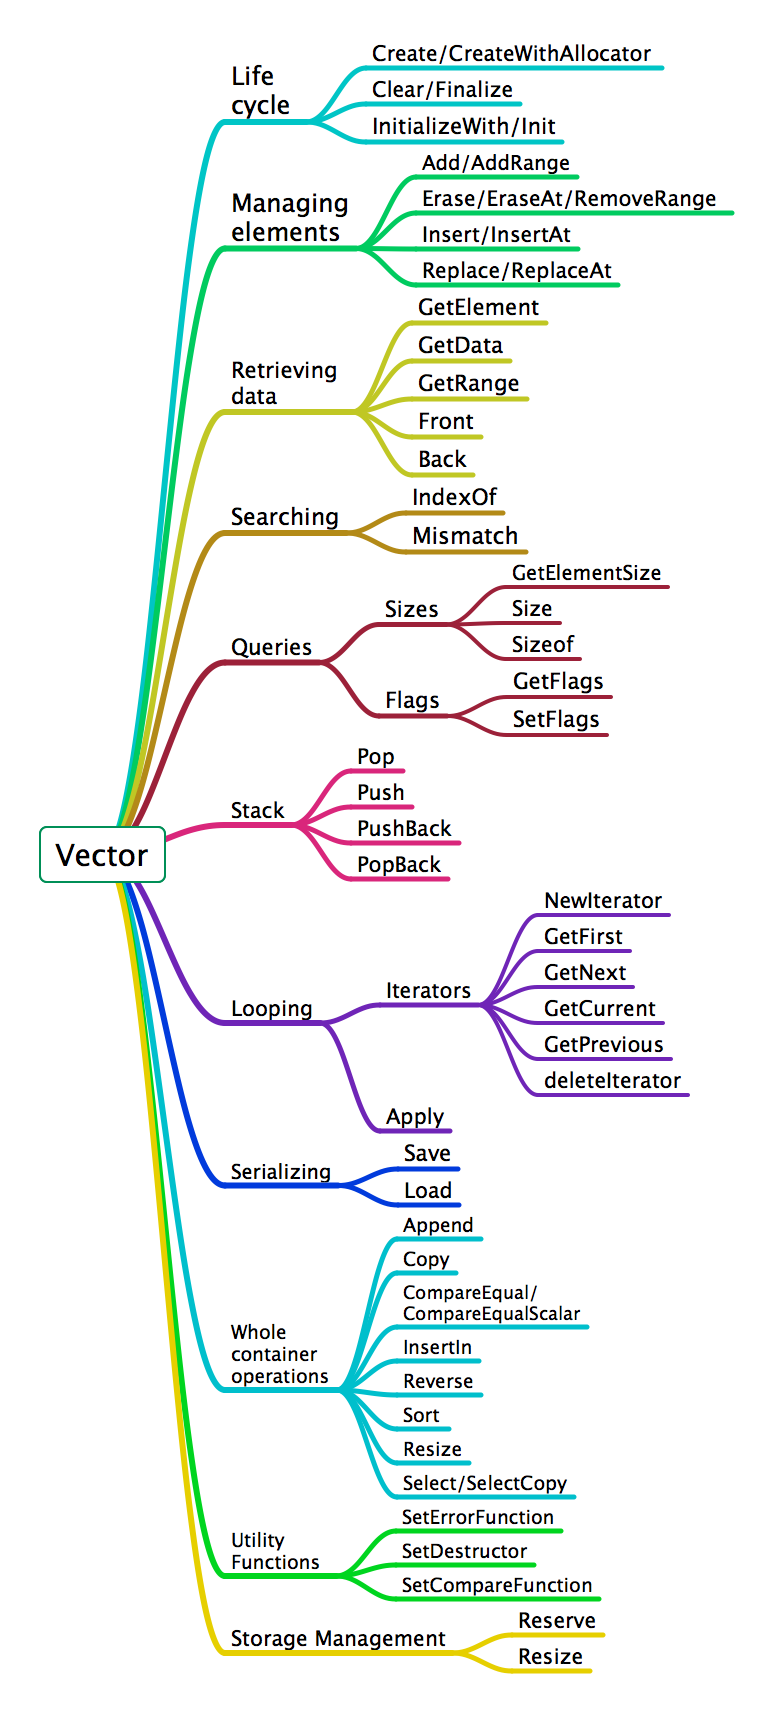
\includegraphics[scale=0.51]{VectorVocabulary.png}
\newpage
\addtolength{\topmargin}{1.8in}
\pagestyle{headings}

\index{Vector}
\subsection{The API}
%-----------------------------------------------------------------------------------------------------
\api{Add}
    int (*Add)(Vector *AL,void *data);
    int (*Add)(TYPEVector, TYPE data);
\end{verbatim} 
\apidescription
Adds the given element to the end of the container. It is the same operations as the PushBack operation. It is assumed that "data" points to a contiguous memory area of at least ElementSize bytes. Returns a value greater than zero if the addition completed successfully, a negative error code otherwise. 
\apierrors
\doerror{BADARG} The vector or the data pointers are \Null.
\doerror{READONLY} The vector is read-only. No modifications allowed.
\doerror{NOMEMORY} Not enough memory to complete the operation.
\returns
A positive number if the operation completed, negative error code otherwise.
\example
    Vector *AL = iVector.Create(sizeof(double));
    double data = 4.5;
    int result = iVector.Add(AL,&data);
    if (result < 0) { /* Error handling */ }

    // Template version
    #include "doubleVector.h"
    doubleVector *AL = idoubleVector.Create();
    int result = idoubleVector.Add(AL,4.5);
    if (result < 0) { /* Error handling */ }
\end{verbatim}
%-----------------------------------------------------------------------------------------------------
\api{AddRange}
    int (*Add)(Vector *AL,size_t n, void *data);
    int (*Add)(TYPEVector *AL,size_t n, TYPE *data);
\end{verbatim} 
\apidescription
Adds the n given elements to the end of the container. It is the same operations as the PushBack operation. It is assumed that "data" points to a contiguous memory area of at least n*ElementSize bytes. Returns a value greater than zero if the addition completed successfully, a negative error code otherwise. If n is zero no error is issued even if the array pointer or the data pointer are \Null.
\apierrors
\doerror{BADARG} The vector or the data pointers are \Null, and n is not zero.
\doerror{READONLY} The vector is read-only. No modifications allowed.
\doerror{NOMEMORY} Not enough memory to complete the operation.
\returns
A positive number if the operation completed, negative error code otherwise.
\example
    Vector *AL;
    double data[] = {4.5, 4.6, 4.7 };
    AL = iVector.Create(sizeof(double),5);
    int result = iVector.Add(AL,3, data);
    if (result < 0) { /* Error handling */ }
    // Template version
    #include "doubleVector.h"
    doubleVector *AL = idoubleVector.Create(5);
    double data[] = {4.5, 4.6, 4.7 };
    int result = idoubleVector.Add(AL,3, data);
    if (result < 0) { /* Error handling */ }
\end{verbatim}
%-----------------------------------------------------------------------------------------------------
\api{Append}
  int (*Append)(Vector *AL1, Vector *AL2);
\end{verbatim}
\apidescription
Adds all elements of AL2 at the end of the first container AL1. The two vectors should contain elements of the same type.
\apierrors
\doerror{BADARG} One of the Vector pointer is \Null.
\doerror{READONLY} The first argument is read-only. No modifications allowed.
\doerror{NOMEMORY} Not enough memory to complete the operation.
\returns
A positive number if the operation completed, negative error code otherwise.
%-----------------------------------------------------------------------------------------------------
\api{Apply}
    int (*Apply)(Vector l,int (Applyfn)(void *,void *),void *arg);
    int (*Apply)(TYPEVector l,int (Applyfn)(TYPE,void *),void *arg);
\end{verbatim} 
\apidescription
Will call the given function for each element of the array. The first argument of the callback function receives an element of the array. The second argument of the callback is the arg argument that the Apply function receives and passes to  the callback. This way some context can be passed to the callback, and from one element to the next.
Note that the result of the callback is not used. This allows all kinds of result types to be accepted after a suitable cast.
If the array is read-only, a copy of the element will be passed to the callback function.
\apierrors
\doerror{BADARG} Either list or Applyfn are \Null.
\doerror{NOMEMORY} The list is read-only and there is no more memory to allocate the buffer to copy each element.
\returns
A positive value if no errors or a negative error code.
\example
    static int Callback(void *pelement,void *pResult)
    {
        double *p = pelement;
        double *result = pResult;
        *result += *p;
        return 1;
    }
    double AddVector(Vector *l) {
        double sum = 0;
        Vector *alist = iVector.Create(sizeof(double),2);
        double d = 2;
        iVector.Add(alist,&d);
        d = 3;
        iVector.Add(alist,&d);
        iList.Apply(alist,Callback,&sum);
        // Here sum should be 5.
        return sum;
    }
    // ------------------------------Template version
    static int Callback(double element,void *pResult)
    {
        double *result = pResult;
        *result += element;
        return 1;
    }
    double AddVector(Vector *l) {
        double sum = 0;
        doubleVector *alist = idoubleVector.Create(2);
        idoubleVector.Add(alist,2);
        idoubleVector.Add(alist,3);
        idoubleList.Apply(alist,Callback,&sum);
        // Here sum should be 5.
        return sum;
    }

\end{verbatim}
%-----------------------------------------------------------------------------------------------------
\api{Back}
void *(*Back)(const Vector *v);
TYPE  (*Back)(const TYPEVector *v);
\end{verbatim}
\apidescription
Returns the last element of the given vector or \Null if the vector is empty.
\apierrors
\doerror{BADARG} The vector pointer is \Null.
\doerror{READONLY} The vector is read only.
\returns
The last element or \Null if the vector is empty or an error occurs.
%-----------------------------------------------------------------------------------------------------
\api{Clear}
    int (*Clear)(Vector *l);
\end{verbatim} 
\apidescription
Erases all stored data and releases the memory associated with it. The vector header will not be destroyed, and its contents will be the same as when the array was initially created. It is an error to use this function when there are still active iterators for the container.
\returns
The result is greater than zero if successful, or an error code if an error occurs. 
\apierrors
\doerror{BADARG} The vector pointer is \Null.
\doerror{READONLY} The vector is read only.
\example
    Vector *Al;
    int m = iVector.Clear(Al);
\end{verbatim}
%-----------------------------------------------------------------------------------------------------
\api{CompareEqual}
Mask *(*CompareEqual)(ValArray *left,ValArray *right,
                       Mask bitarray);
\end{verbatim}
\apidescription
Assigns to each element of the mask the result of comparing the corresponding elements of the left and right arrays. Conceptually this operation is: \begin{verbatim}
Mask[i] = (left[i] == right[i])
\end{verbatim} 
If the mask argument is \Null it will be allocated and returned. 
The allocator used is the global memory manager. 
If it is not \Null it should contain at least enough positions to hold the data. If it doesn't it will be finalized using \verb,iMask.Finalize, and 
allocated with the necessary length.
\apierrors
\doerror{NOMEMORY}. The given byte array argument was \Null but there is no memory to allocate the result.
\doerror{BADARG} The given mask hasn't enough positions available.
\doerror{INCOMPATIBLE} The arrays are of different length.
\returns A pointer to the bitarray passed or allocated, or \Null if an error occurs.
%-----------------------------------------------------------------------------------------------------
\api{CompareEqualScalar}
Mask *(*CompareEqual)(const Vector *left,const void *right,
                       Mask *bitarray);
\end{verbatim}
\apidescription
Assigns to each element of the mask the result of comparing the elements of the left array with the right argument. 
Conceptually this operation is: 
\begin{verbatim}
bit[i] = (left[i] == right)
\end{verbatim} 
If the bitarray argument is \Null it will be allocated and returned. The allocator used is the one from the left argument. If it is not \Null it will be allocated if its length is less than the needed length.
\apierrors
\doerror{NOMEMORY}. The given byte array argument was \Null but there is no memory to allocate the result.
\returns A pointer to the bitarray or \Null if an error occurs.
%-----------------------------------------------------------------------------------------------------
\api{Contains}
    int (*Contains)(Vector *a,void *data);
    int (*Contains)(TYPEVector *a,TYPE data);
\end{verbatim} 
\apidescription
Searches the given data in the array. The "data" argument is supposed to point to an element at least ElementSize bytes. The array's comparison function is used for determining if two elements are equal. This comparison function defaults to memcmp.
\apierrors
\doerror{BADARG} Either array or data are \Null.
\returns
One if the given data is stored in the array, zero otherwise. If either the data pointer or the array pointer are \Null it returns a negative error code.
\example
    Vector *a = iVector.Create(sizeof(double),2);
    double data = 78.67;
    int r = iVector.Contains(a,&data);
    // ---------------------------Template version
    doubleVector *a = iVector.Create(2);
    int r = iVector.Contains(a,78.67);
\end{verbatim}
%-----------------------------------------------------------------------------------------------------
\api{Copy}
    Vector *(*Copy)(Vector *A);
\end{verbatim} 
\apidescription
A shallow copy of the given array is performed. Only ElementSize bytes will be copied for each element. If the element contains pointers, only the pointers are copied, not the objects they point to. The new memory will be allocated using the given array's allocator.
\apierrors
\doerror{NOMEMORY} There is not enough memory to complete the operation.
\doerror{BADARG} The given vector pointer is \Null.
\example
    Vector *newVector,*OldVector;
    newVector = iVector.Copy(OldVector);
\end{verbatim}
%-----------------------------------------------------------------------------------------------------
\api{CopyElement}
    Vector *(*Copy)(const Vector *A,size_t idx,void *result);
\end{verbatim} 
\apidescription
The element at the given index is copied into the output buffer that should be at least big enough to hold one element. If the index is bigger
than the number of elements the error function is called. If it returns a valid pointer (not \Null) it is assumed that this is a pointer to a valid
element that should be copied into the output buffer.
\apierrors
If the \verb,idx, argument is out of range the \verb,CopyElement, function calls the vector error function. If the error function returns a result
different than \Null, the function assumes that it is a pointer to some value that should be copied into the result buffer.
\doerror{INDEX} The index is out of bounds.
\doerror{BADARG} The given vector pointer is \Null.
\example
    Vector *V;
    char buffer[16];
    newVector = iVector.CopyElement(V,3,buffer);
\end{verbatim}
%------------------------------------------------------------------------------------------------------
\api{CopyTo}
void **(*CopyTo)(Vector *AL);
\end{verbatim}
\apidescription
Copies the whole contents of the given array into a table of pointers to newly allocated elements, finished by a \Null pointer.
\apierrors
\doerror{BADARG} The iterator pointer is \Null.
\doerror{NOMEMORY} There is not enough memory to complete the operation.
\returns
A pointer to a table of pointers or \Null if an error occurs.
\api{deleteIterator}
    int deleteIterator(Iterator *it);
\end{verbatim}
\apidescription
Reclaims the memory used by the given iterator object
\returns 
Integer smaller than zero with error code or a positive number when the operation completes.
\apierrors
\doerror{BADARG} The iterator pointer is \Null.
%-----------------------------------------------------------------------------------------------------
\api{Create}
    Vector *(*Create)(size_t element_size,size_t startsize);
    TYPEVector *(*Create)(size_t startsize);
\end{verbatim} 
\apidescription
The creation function returns an empty array, initialized with all the default values.
The current memory manager is used to allocate the space needed for the header. The array is supposed to contain elements of the same size. If the elements you want to store are of different size, use a pointer to them, and create the array with sizeof(void *) as the size parameter.

\returns
A pointer to a newly created array or \Null if an error occurs.
\apierrors
\doerror{NOMEMORY} There is not enough memory to complete the operation.
\doerror{BADARG} The given element size is zero.

Any errors provoke the call the current default error function of the library since this is the creation function.
\example
    Vector *DArray = iVector.Create(sizeof(double),100);
\end{verbatim}
%-----------------------------------------------------------------------------------------------------
\api{CreateWithAllocator}
Vector *(*CreateWithAllocator)(size_t elementsize,
                    size_t startsize,ContainerAllocator *allocator);
\end{verbatim}
\apidescription
This function is identical to \texttt{Create} with the difference that it accepts a pointer to an allocator object. Actually, \texttt{Create} can
be written as:\par\noindent
\texttt{return CreateWithAllocator(elementsize,startsize,CurrentAllocator);}
%-----------------------------------------------------------------------------------------------------
\api{Equal}
    int (*Equal)(Vector *first,Vector *second);
\end{verbatim}
\apidescription
Compares the given arrays. If they differ in their length, flags, or element size they compare unequal. If any of their elements differ, they compare unequal.
If both first and second are \Null they compare equal. 
\apierrors
None
\returns
The result is one if the vectors are equal, zero otherwise.
%-----------------------------------------------------------------------------------------------------
\api{Erase}
    int (*Erase)(Vector *AL,void *data);
    int (*Erase)(TYPEVector *AL,TYPE data);
\end{verbatim}
\apidescription
Removes from the vector the element that matches the given data, that is assumed to be a pointer to an element.
\returns
A negative error code if an error occurred, or a positive value that indicates that at least one match was found and the elements were removed. 
If the element is not in the vector the result value is \notfound.
\apierrors
\doerror{BADARG} One or both arguments are \Null.

\example
    double d = 2.3;
    Vector *AL;
    int r = iVector.Erase(AL,&d);
    if (r > 0)
        printf("2.3 erased|n");
    else if (r == 0)
        printf("No element with value 2.3 present\n");
    else
        printf("error code %d\n",r);
\end{verbatim}
%-----------------------------------------------------------------------------------------------------
\api{EraseAll}
    int (*EraseAll)(Vector *v,const void *data);
    int (*EraseAll)(TYPEVector *v,const TYPE data);    
\end{verbatim}
\apidescription
Removes from the list all elements that match the given data, that is assumed to be a pointer to an element.
\returns
A negative error code if an error occurred, or a positive value that indicates that at least a match was found and the element was removed. If the 
element is not in the list the result is \notfound.
\apierrors
\doerror{BADARG} One or both arguments are \Null.
%-----------------------------------------------------------------------------------------------------
\api{EraseAt}
    int (*EraseAt)(Vector *AL,size_t idx);
\end{verbatim}
\apidescription
Removes from the array the element at the given position.

\returns
A negative error code if an error occurred or a positive value that indicates that the element was removed.

\apierrors
\doerror{BADARG} The given vector pointer is \Null.
\doerror{INDEX} The given position is out of bounds.

\example
    Vector *AL;
    int r = iVector.EraseAt(AL,2);
    if (r > 0)
        printf("Element at position 2 erased\n");
    else
        printf("Error code %d\n",r);
\end{verbatim}
\api{Finalize}
    int (*Finalize)(Vector *AL);
\end{verbatim}
\apidescription
Reclaims all memory used by the container, including the array header object itself.
\apierrors
\doerror{BADARG} The given vector pointer is \Null.
\doerror{READONLY} The container is read-only. No modifications allowed.
\returns
A positive value means the operation completed. A negative error code indicates failure.
\example
    Vector *AL;
    int r = iVector.Finalize(AL);
    if (r < 0) { /* error handling */ }
\end{verbatim}
%-----------------------------------------------------------------------------------------------------
\api{Front}
void *(*Front)(const Vector *v);
TYPE  (*Front)(const TYPEVector *v);
\end{verbatim}
\apidescription
Returns the first element of the given vector or \Null if the vector is empty.
\apierrors
\doerror{BADARG} The vector pointer is \Null.
\doerror{READONLY} The vector is read only.
\returns
The first element or \Null if the vector is empty or an error occurs.
%-----------------------------------------------------------------------------------------------------
\api{GetCapacity}
    size_t (*GetCapacity)(const Vector *AL);
\end{verbatim}
\apidescription
Returns the number of elements the array can hold before  it needs to reallocate its data\footnote{A similar function exists in the C++ STL: 
\texttt{max\_size()}}.
\apierrors
\doerror{BADARG} The given array is \Null.
\returns
The array capacity or zero if there was an error.
%-----------------------------------------------------------------------------------------------------
\api{GetElementSize}
    size_t (*GetElementSize)(const Vector *AL);
\end{verbatim}
\apidescription
Retrieves the size of the elements stored in the given vector. Note that this value can be different than the value given to the creation function because of alignment requirements. In template containers this function returns
\verb,sizeof(TYPE),.
\apierrors
\doerror{BADARG} The given vector pointer is \Null.

\returns
The element size.
\example
    Vector *AL;
    size_t siz = iVector.GetElementSize(AL);
\end{verbatim}
%-----------------------------------------------------------------------------------------------------
\api{GetData}
void **(*GetData)(const Vector *AL);
\end{verbatim}
\apidescription
Returns a pointer to the data area of the container, or \Null if an error occurs.
\apierrors
\doerror{READONLY} The container is read-only.
\doerror{BADARG} The given pointer is \Null
\returns The pointer to the array's data or \Null.
%-----------------------------------------------------------------------------------------------------
\api{GetElement}
    void *(*GetElement)(Vector *AL,size_t idx);
    TYPE *(*GetElement)(TYPEVector *AL,size_t idx);
\end{verbatim}
\apidescription
Returns a read only pointer to the element at the given index, or \Null if the operation failed.  This function will return \Null if the vector is read only. If the index is greater than the number of elements, the error function will be called. If the error function returns a valid pointer
(not \Null) the result will be that pointer. This allows the construction of infinite arrays, or sparse arrays, etc. By default, the error function
returns always \Null.
 
Use the CopyElement function to get a read/write copy of an element of the vector.

\apierrors
\doerror{BADARG}    The given array pointer is \Null.
\doerror{INDEX}    The given position is out of bounds.
\doerror{READONLY}    The array is read only.
\example
    Vector *AL;
    double *d = iVector.GetElement(AL,3);
    if (d == NULL) { /* Error handling */ }
\end{verbatim}
%-----------------------------------------------------------------------------------------------------
\api{GetFlags / SetFlags}
    unsigned (*GetFlags)(Vector *AL);
    unsigned (*SetFlags)(Vector *AL,unsigned newFlags);
\end{verbatim}
\apidescription
GetFlags returns the state of the container flags, SetFlags sets the flags to a new value and returns the old value. 

The Vector container supports the following flags:

\textsc{CONTAINER\_READONLY}
If this flag is set, no modifications to the container are allowed, and the Clear and Finalize functions will not work. The GetElement function will always return \Null. You should use the CopyElement function to access the data
%-----------------------------------------------------------------------------------------------------
\api{GetRange}
    Vector *(*GetRange)(Vector *AL,size_t start,size_t end);
\end{verbatim}
\apidescription
Selects a series of consecutive elements starting at position start and ending at position end.  Both the elements at start and end are included in the result.
If start > end or start > Size(AL), \Null is returned. If end is bigger than the number of elements in the vector AL, only elements up to the number of elements will be used.
The selected elements are copied into a new array. The original array remains unchanged.
\apierrors
\doerror{BADARG} The given array pointer or the element given are \Null
\returns A pointer to a new vector containing the selected elements or \Null if an error occurs.
\example
    Vector *AL;
    Vector *range = iVector.GetRange(AL,2,5);
    if (range == NULL) { /* Error handling */ }
\end{verbatim}
%-----------------------------------------------------------------------------------------------------
\api{IndexIn}
Vector *(*IndexIn)(Vector *SC,Vector *AL);
\end{verbatim}
\apidescription
Returns an array built from indexing the first argument ("SC") with the array of indexes "AL" that should be an array of size\_t elements. The number of elements of the resulting array is equal to the number of elements of the indexes array.
\apierrors
\doerror{BADARG} The given array pointer or the indexes array are \Null.
\doerror{INDEX} Any given position is out of bounds.
\doerror{NOMEMORY} There is not enough memory to complete the operation.
\returns
A new array or \Null if an error occurs. No partial results are returned. If any index is out of bounds the whole operation fails.

\api{IndexOf}
int (*IndexOf)(Vector *l,void *data,void *ExtraArgs,size_t *result);
int (*IndexOf)(TYPEVector *l,TYPE data,void *ExtraArgs,size_t *result);
\end{verbatim}
\apidescription
Searches for an element in the array. If found its zero based index is returned in the pointer "result". Otherwise the result of the search is \notfound. The "extraArgs" argument will be passed to the comparison function, that is used to compare elements.
\apierrors
\doerror{BADARG} The given array pointer or the element given are \Null.
\returns
A positive number if the element is found, or a negative number containing an error code or the negative constant \notfound.
\example
    Vector *AL;
    double data = 6.8;
    size_t pos;
    int r = iVector.IndexOf(AL,&data,NULL,&pos);
    if (r == CONTAINER_ERROR_NOTFOUND)
        printf("Not found\n");
\end{verbatim}

\api{InsertAt}
    int (*InsertAt)(Vector *AL,size_t idx,void *newData);
    int (*InsertAt)(TYPEVector *AL,size_t idx,TYPE newData);
\end{verbatim}
\apidescription
Inserts the new element. The new element will have the given index, that can go from zero to the vector count inclusive, i.e. one more than the number of elements in the vector. If the index is out of bounds, the vector error function is called. If the function returns a valid pointer (a pointer
different than \Null) it will be assumed that the vector should be increased to the index given. The vector is resized and the data is inserted
at the requested position. This allows the implementation of infinite vectors, sparse vectors, and other data structures.
\apierrors
When this API detects an index error, it calls the error function. If the error function returns a pointer different from \Null, the API will extend
the requested vector to make possible the insertion. If the API is unable to extend the vector and error is returned and the vector remains unchanged.

\doerror{BADARG} The given vector pointer or the element given are \Null.
\doerror{READONLY} The vector is read only.
\doerror{INDEX} The given position is out of bounds.
\doerror{NOMEMORY} There is not enough memory to complete the operation.

\returns
A positive value if the operation succeeded, or a negative error code if the operation failed.
\example
    double d = 2.7;
    Vector *AL = iVector.Create(sizeof(double),3);
    int r = iVector.InsertAt(AL,2,&d);
    if (r < 0) { /* Error handling */ }
    else { /* Normal processing */  }
    // --------------------------Template version
    doubleVector *AL = idoubleVector.Create(3);
    int r = idoubleVector.InsertAt(AL,2,2.7);
    if (r < 0) { /* Error handling */ }
    else { /* Normal processing */  }

\end{verbatim}

\api{InsertIn}
    int (*InsertIn)(Vector *Destination, size_t pos, Vector *src);
\end{verbatim}
\apidescription
Inserts the array given in  its third argument at the given position in the array pointed to by its first argument. The data is copied, and the source argument is not modified in any way. Both arrays must have elements of the same type. The library only tests the size of each one.
\apierrors
\doerror{BADARG} The source or the destination vectors are \Null.
\doerror{READONLY} The destination vector is read only.
\doerror{INDEX} The given position is out of bounds.
\doerror{NOMEMORY} There is not enough memory to complete the operation.
\doerror{INCOMPATIBLE} The vectors store elements of different size.
\returns
A positive value if the operation succeeded, or a negative error code if the operation failed.
\example
#include <containers.h>
static void PrintVector(Vector *AL)
{
    size_t i;
    printf("Count %ld, Capacity %ld\n",(long)iVector.Size(AL),
                                  (long)iVector.GetCapacity(AL));
    for (i=0; i<iVector.Size(AL);i++) {
        printf("%g ",*(double *)iVector.GetElement(AL,i));
    }
    printf("\n");
}

static void FillVector(Vector * AL,int start)
{
    size_t i;

    for (i=0; i<10;i++) {
        double d = i+start;
        iVector.Add(AL,&d);
    }
}

int main(void)
{
    Vector *AL = iVector.Create(sizeof(double),10);
    Vector *AL1 =iVector.Create(sizeof(double),10);
    FillVector(AL,0);
    FillVector(AL1,100);
    iVector.InsertIn(AL,5,AL1);
    PrintVector(AL);
    return 0;
}
OUTPUT:
Count 20, Capacity 20
0 1 2 3 4 100 101 102 103 104 105 106 107 108 109 5 6 7 8 9
---------------------------------------------Template version
#include <containers.h>
#include "doublevector.h"
static void PrintVector(doubleVector *AL)
{
    size_t i;
    printf("Count %ld, Capacity %ld\n",(long)iVector.Size(AL),
                                  (long)iVector.GetCapacity(AL));
    for (i=0; i<iVector.Size(AL);i++) {
        printf("%g ",idoubleVector.GetElement(AL,i));
    }
    printf("\n");
}

static void FillVector(Vector * AL,int start)
{
    size_t i;

    for (i=0; i<10;i++) {
        idoubleVector.Add(AL,i+start);
    }
}

int main(void)
{
    Vector *AL = idoubleVector.Create(10);
    Vector *AL1 =idoubleVector.Create(10);
    FillVector(AL,0);
    FillVector(AL1,100);
    iVector.InsertIn(AL,5,AL1);
    PrintVector(AL);
    return 0;
}
OUTPUT:
Count 20, Capacity 20
0 1 2 3 4 100 101 102 103 104 105 106 107 108 109 5 6 7 8 9

\end{verbatim}
\api{Load}
   Vector *(*Load)(FILE *stream,ReadFunction readFn,void *arg);
\end{verbatim}
\apidescription
Reads an array previously saved with the Save function from the stream pointed to by stream. If readFn is not \Null, it will be used to read each element. The \verb,arg, argument will be passed to the read function. If the read function is \Null, this argument is ignored and a default read function is used.
\apierrors
\doerror{BADARG} The given stream pointer is \Null.
\doerror{NOMEMORY} There is not enough memory to complete the operation.

\returns
A new array or \Null if the operation could not be completed. Note that the function pointers in the array are NOT saved, nor any special allocator that was in the original vector. Those values will be the values by default. To rebuild the original state the user should replace the pointers again in the new array.
%--------------------------------------------------------------------------------------------------------------------------
\api{NewIterator}
    Iterator *(*NewIterator)(Vector *AL);
\end{verbatim}
\apidescription
Allocates and initializes a new iterator object to iterate this array.
\apierrors
If no more memory is available it returns \Null.
\returns
A pointer to a new iterator or \Null if there is no more memory left.
\example
    Vector *AL;
    Iterator *it = iVector.NewIterator(AL);
    double *d;
    for (d=it->GetFirst(it); d != NULL; d = it->GetNext(it)) {
        double val = *d;
        // Work with the value here
    }
    iVector.deleteIterator(it);
\end{verbatim}
%--------------------------------------------------------------------------------------------------------------------------
\api{Mismatch}
int (*Mismatch)(const Vector *a1,const Vector *a2,
                                         size_t *mismatch);
\end{verbatim}
\apidescription
Returns the index of the first element that is different when comparing both arrays in the passed pointer \textsl{mismatch}. If one array is shorter than the other the comparison stops
when the last element from the shorter array is compared. The comparison stops when the first difference is spotted.
\apierrors
\doerror{BADARG} Any of the arguments is \Null.
\doerror{INCOMPATIBLE} The containers have different comparison functions or store elements of different size.
\returns
If a mismatch is found the result is greater than zero and the \textsl{mismatch} argument will contain the index of the first element that compared 
unequal. This will be always the case for arrays of different length.

If both arrays are the same length and no differences are found the result is zero and the value pointed to by the 
\textsl{mismatch} argument is one more than the length of the arrays.

If an error occurs, a negative error code is returned. The \textsl{mismatch} argument contains zero.
%--------------------------------------------------------------------------------------------------------------------------
\api{PopBack}
    int (*PopBack)(Vector *AL,void *result);
    int (*PopBack)(TYPEVector *AL,TYPE *result);
\end{verbatim}
\apidescription
Copies the last element into the given result buffer and deletes the element from the container. If the result buffer is \Null, no copy is performed.
\apierrors
\doerror{BADARG} The array is \Null.
\doerror{READONLY} The array is read only.

\returns
A negative value if an error occurs, zero if the array is empty or greater than zero if the operation succeeded.
%--------------------------------------------------------------------------------------------------------------------------
\api{RemoveRange}
int (*RemoveRange)(Vector *SC,size_t start,size_t end);
\end{verbatim}
\apidescription
Removes all elements having an index equal or greater than\param{start} and less than\param{end}. If\param{end} is greater than the number of elements 
in the collection it will be adjusted to one more than the number of elements. If\param{start} is bigger than\param{end} the range is still valid and
starts with the value of\param{end} and ends with the value of\param{start}.
\apierrors
\doerror{BADARG} The vector pointer is \Null.
\returns
Zero if the vector is empty. Otherwise returns a positive number for success, a negative error code in case of an error.
%--------------------------------------------------------------------------------------------------------------------------
\api{ReplaceAt}
    int (*ReplaceAt)(Vector *AL,size_t idx,void *newData);
    int (*ReplaceAt)(TYPEVector *AL,size_t idx,TYPE newData);
\end{verbatim}
\apidescription
Replaces the array element at position idx with the new data starting at the position pointed to by "newData" and extending ElementSize bytes.
\apierrors
\doerror{BADARG} The array or the new element pointer are \Null.
\doerror{READONLY} The array is read only.
\doerror{INDEX} The given position is out of bounds.
\returns
A negative error code if an error occurs, or a positive value if the operation succeeded.
\example
    Vector *AL = iVector.Create(sizeof(double),2);
    double d = 6.7;
    int r = iVector.ReplaceAt(AL,2,&d);
    if (r < 0) { /* Error handling */ }
    // --------------------------------Template version
    doubleVector *AL = idoubleVector.Create(2);
    int r = idoubleVector.ReplaceAt(AL,2,6.7);
    if (r < 0) { /* Error handling */ }
\end{verbatim}
%--------------------------------------------------------------------------------------------------------------------------
\api{Reserve}
int (*Reserve)(Vector *AL, size_t newSize);
\end{verbatim}
\apidescription
The capacity of the vector is increased at least by the given amount in preparation for a planned increase in elements. The size is in element
units.
\apierrors
\doerror{BADARG} The array pointer is \Null.
\doerror{READONLY} The array is read only.
\doerror{NOMEMORY} Not enough memory is available
\returns A positive number if the space could be reserved, a negative error code if not.
%--------------------------------------------------------------------------------------------------------------------------
\api{Resize}
int (*Resize)(Vector *AL, size_t newSize);
\end{verbatim}
\apidescription
Resizes the given vector to the new capacity, expressed in element units. If the new capacity is smaller than the elements in 
the vector some elements will be erased.
For each erased element its destructor (if any) is called. If the requested \verb,newSize, argument is equal to the number of elements in the 
container, all storage beyond what is needed to store exactly \verb,newSize, elements, is released.
This allows to signal the library that the extra storage is no longer needed\footnote{The latest
C++ standard adds this operation calling it \texttt{std::vector::shrink\_to\_fit}}.
\begin{verbatim}
iVector.Resize(vec,iVector.Size(vec));
\end{verbatim}

Obviously under some implementations it is maybe impossible to allocate \textbf{exactly} the space needed, for instance because space can be only 
allocated in chunks bigger than the element size of the vector. In those cases only a "best effort" will be done and the used storage will be reduced 
to a minimum.
If an error occurs, and the container can't be resized, no changes occur and the container is left unmodified.
\apierrors
\doerror{BADARG} The array pointer is \Null.
\doerror{READONLY} The array is read only.
\doerror{NOMEMORY} Not enough memory is available
\returns
A negative error code if an error occurs, or a positive value if the operation succeeded. If the requested capacity is equal to the current
capacity  the result is zero.
%--------------------------------------------------------------------------------------------------------------------------
\api{Reverse}
int (*Reverse)(Vector *AL);
\end{verbatim}
\apidescription
Reverses the order of the elements of the given Vector.
\apierrors
\doerror{BADARG} The array pointer is \Null.
\doerror{READONLY} The array is read only.
\doerror{NOMEMORY} Not enough memory for intermediate storage available
\returns
A negative error code if an error occurs, or a positive value if the operation succeeded.
%--------------------------------------------------------------------------------------------------------------------------
\api{RotateRight}
    int (*RotateRight)(Vector *src,size_t n);
\end{verbatim}
\apidescription
Rotates right the array by the indicated amount. The last n elements will be written to the start of
the array, and the rest will be shifted right.
\apierrors
\doerror{BADARG} The array pointer is \Null.
\doerror{READONLY} The array is read only.
\doerror{NOMEMORY} Not enough memory is available
\returns A positive number if something was moved, zero otherwise (the input was zero or a 
modulo of the array size).

%--------------------------------------------------------------------------------------------------------------------------
\api{RotateLeft}
    int (*RotateLeft)(Vector *src,size_t n);
\end{verbatim}
\apidescription
Rotates left the array by the indicated amount. The first n elements will be written to the end of
the array, and the rest will be shifted left to fill the empty n places.
\apierrors
\doerror{BADARG} The array pointer is \Null.
\doerror{READONLY} The array is read only.
\doerror{NOMEMORY} Not enough memory for intermediate storage available
\returns A positive number if something was moved, zero otherwise (the input was zero or a 
modulo of the array size), or an error code less than zero if an error occurs.
%--------------------------------------------------------------------------------------------------------------------------
\api{Save}
int (*Save)(const Vector *AL, FILE *out, SaveFunction Fn, void *arg);
\end{verbatim}
\apidescription
The contents of the given vector are saved into the given stream. If the save function pointer is not \Null, it will be used to save the contents of each element and will receive the arg argument passed to Save, together with the output stream. Otherwise a default save function will be used and arg will be ignored.
The output stream must be opened for writing and must be in binary mode.
\apierrors
\doerror{BADARG} The array pointer or the stream pointer are \Null.
EOF A disk input/output error occurred.

\returns
A positive value if the operation completed, a negative value or EOF otherwise.
\example
    Vector *AL;
    FILE *outFile;
    if (iVector.Save(AL,outFile,NULL,NULL) < 0) { 
        /* Handle error here */
    }
\end{verbatim}
%--------------------------------------------------------------------------------------------------------------------------
\api{SearchWithKey}
int (*SearchWithKey)(Vector *vec,size_t startByte,size_t sizeKey,
                     size_t startIndex,void *item, size_t*result);
\end{verbatim}
\apidescription
This function searches the vector for a match in a region of the stored objects, ignoring the rest of the data. It will start at the object with \textsl{startIndex} and compare (using memcmp) the specified region of each object. The region of interest within the stored object is specified 
by a byte offset and a size.
If a match is found the search stops and the zero based index of the object will
be written into the \textsl{result} pointer. If the index of the start of the iteration is bigger than the number of elements in the array nothing
is searched and the result is zero.

If the sum of \textsl{startByte} and \textsl{sizeKey} is bigger than the size of the elements stored, the comparison will start at the given offset but will stop
at the end of the stored element.

\apierrors
\doerror{BADARG} The array or the item element pointers are \Null.
\returns
A negative error code if an error occurs, zero if no match was found, or a positive number indicating that a match was found. The given index pointer is
modified only if a match is found.
%--------------------------------------------------------------------------------------------------------------------------
\api{Select}
int (*Select)(Vector *v,Mask *m);
\end{verbatim}
\apidescription
Using the given mask, the elements where the corresponding mask element is zero are eliminated, those with a mask
value different of zero are retained. The mask must have the same length as the array.
\apierrors
\doerror{INCOMPATIBLE} The mask and the array are of different length.
\returns A positive value for success, or a negative error code otherwise.
%--------------------------------------------------------------------------------------------------------------------------
\api{SelectCopy}
Vector *(*SelectCopy)(Vector *v,Mask *m);
\end{verbatim}
\apidescription
Using the given mask, the elements where the corresponding mask element is different from zero are copied into a new array, those with a mask
value different of zero are ignored. The mask must have the same length as the array.
\apierrors
\doerror{INCOMPATIBLE} The mask and the array are of different length.
\returns A positive value for success, or a negative error code otherwise.
%--------------------------------------------------------------------------------------------------------------------------
\api{SetCapacity}
int (*SetCapacity)(Vector *AL,size_t newCapacity);
\end{verbatim}
\apidescription
Resizes the given Vector to a new value. The new capacity means there will be that number of elements allocated, avoiding costly resizing operations when new elements are added to the Vector. If the number given is less than the number of elements present in the array, elements are discarded from the end of the array.
\apierrors
\doerror{BADARG} The Vector pointer is \Null.
\doerror{READONLY} The array is read only.
\returns A positive value if resizing was completed, a negative error code otherwise.

%--------------------------------------------------------------------------------------------------------------------------
\api{SetCompareFunction}
CompareFunction (*SetCompareFunction)(Vector *AL,
                                         CompareFunction f);
\end{verbatim}
\apidescription
if the f argument is non \Null, it sets the array comparison function to f.
\apierrors
\doerror{BADARG} The array pointer is \Null.
\doerror{READONLY} The array is read only and the function argument is not \Null.
\returns
The old value of the comparison function.
\example
    ErrorFunction fn,newfn;
    Vector *AL;
    fn = iVector.SetErrorFunction(AL,newfn);
\end{verbatim}
%--------------------------------------------------------------------------------------------------------------------------
\api{SetDestructor}
DestructorFunction (*SetDestructor)(Vector *v,DestructorFunction fn);
\end{verbatim}
\apidescription Sets the destructor function to its given argument. If the function argument is \Null nothing is changed and the call is interpreted as a query since the return value is the current value of the destructor function. If the vector argument is \Null, the result is \Null.
\returns The old value of the destructor.

%--------------------------------------------------------------------------------------------------------------------------
\api{SetErrorFunction}
    ErrorFunction (*SetErrorFunction)(Vector *V,ErrorFunction); 
\end{verbatim}
\apidescription
Replaces the current error function  for the given vector with the new error function if the\param{ErrorFunction}parameter is different from \Null. If 
the\param{V}parameter is \Null the function returns the value of the current default error function.
\apierrors
\doerror{BADARG} The vector pointer is \Null.
\doerror{READONLY} The vector is read only and the function argument is not \Null.
\returns
The old value of the error function or \Null if there is an error.

%--------------------------------------------------------------------------------------------------------------------------
\api{Size}
    size_t (*Size)(const Vector *AL);
\end{verbatim}
\apidescription
Returns the number of elements stored in the array.
\example
    Vector *AL;
    size_t elem = iVector.Size(AL);
\end{verbatim}

%--------------------------------------------------------------------------------------------------------------------------
\api{Sizeof}
    size_t (*Sizeof)(Vector *AL);
\end{verbatim}
\apidescription
Returns the total size in bytes of the vector, including the header, and all data stored in it. If the argument is \Null, the size of the header only is returned.
\returns
The number of bytes used by the vector or the size of the Vector header if the argument is \Null.
\example
    Vector *AL;
    size_t  size = iVector.Sizeof(AL);
\end{verbatim}

%--------------------------------------------------------------------------------------------------------------------------
\api{Sort}
    int Sort(Vector *AL);
\end{verbatim}
\apidescription
Sorts the given array using the its comparison function. The order of the original array is destroyed. You should copy it if you want to preserve it. 
\returns
A positive number if sorting succeeded, a negative error code if not.
\example
    Vector *AL;
    if (iVector.Sort(AL) < 0) { /* Error handling */ }
\end{verbatim}
%--------------------------------------------------------------------------------------------------------------------------
%                                                   Bit strings
%--------------------------------------------------------------------------------------------------------------------------
\newpage
\section{The bit-string container: iBitString}
\renewcommand{\container}{BitString}
\index{BitString}
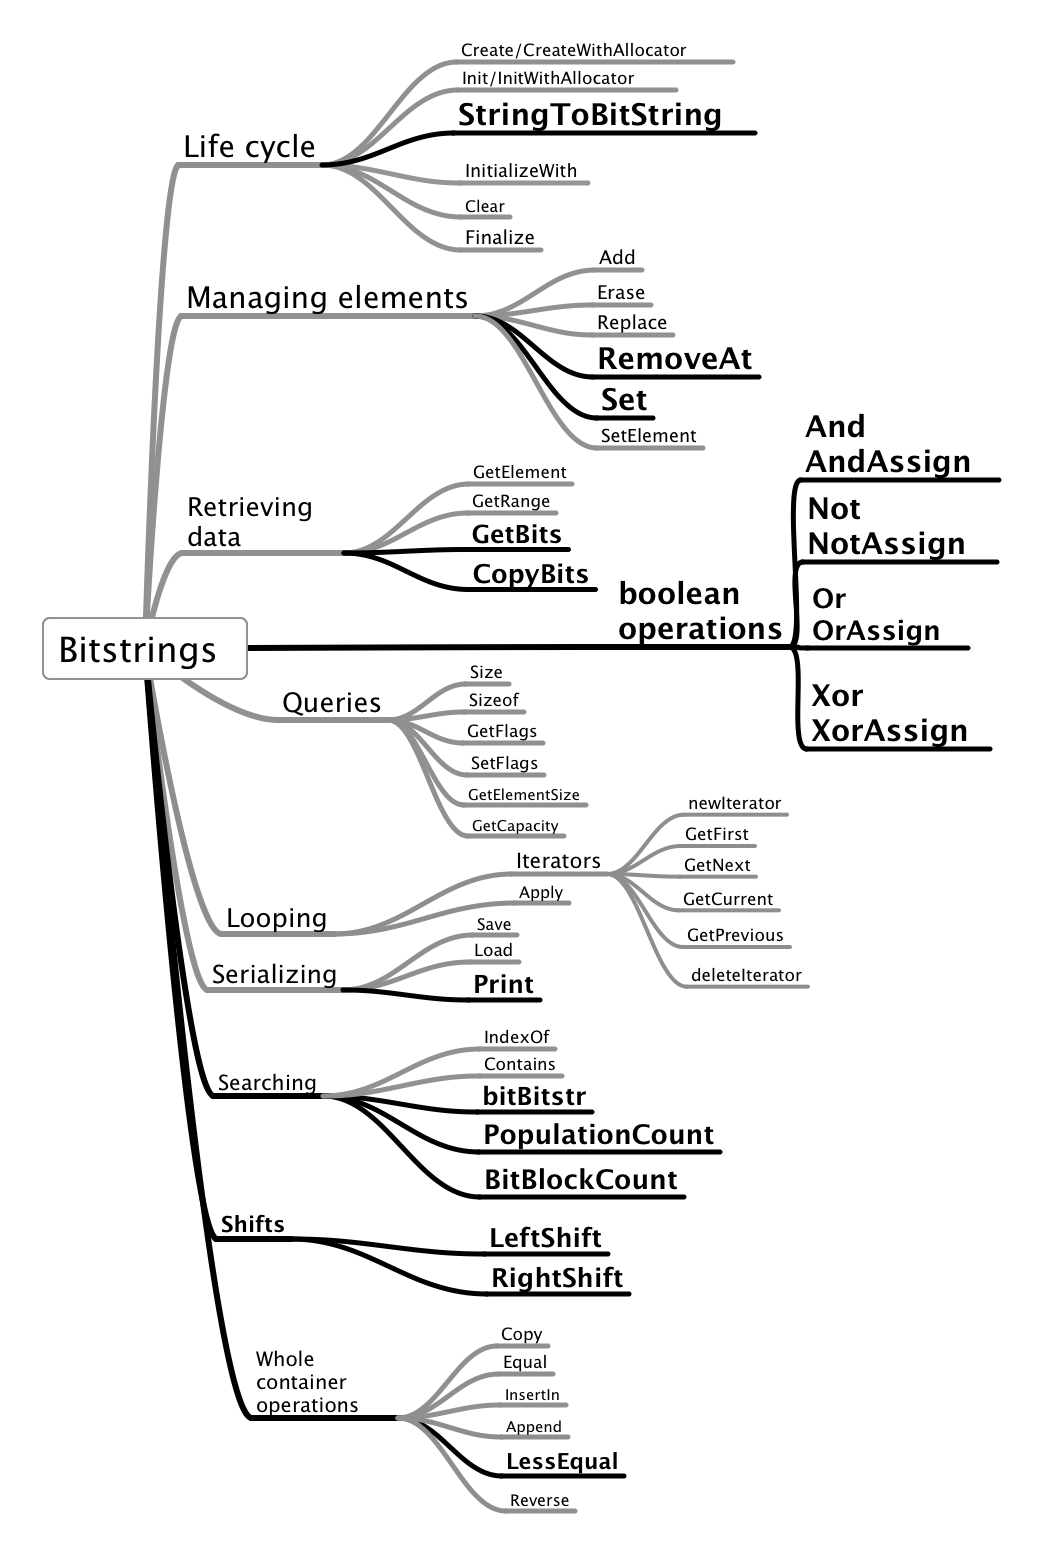
\includegraphics[scale=0.37]{bitstrings.png}\par
\hfill BitString vocabulary. Specific items are in bold.\par
A bit string is a derivation from the Vector container, specialized to hold a sequence of bits. It is a sequential container designed to save space in the storage of boolean values
\footnote{
The equivalent in C\# is the \texttt{BitArray} class in \texttt{System.Collections}. In Java the equivalent is the BitSet class.
}. 
\subsection{The interface}
\index{iBitString}
\begin{verbatim}
typedef struct tagBitStringInterface {
   int (*Add)(BitString *BitStr,int);
   int (*AddRange)(BitString *b, size_t bitSize, void *data);
   BitString *(*And)(BitString *bsl,BitString *bsr);
   int (*AndAssign)(BitString *bsl,BitString *bsr);
   int (*Append)(BitString *left,BitString *right);
   int (*Apply)(BitString *BitStr,int (*Applyfn)(int ,void * arg),
        void *arg);
   uintmax_t (*BitBlockCount)(BitString *b);
   int (*BitLeftShift)(BitString *bs,size_t shift);
   int (*BitRightShift)(BitString *bs,size_t shift);
   int (*Clear)(BitString *BitStr);
   int (*Contains)(BitString *BitStr,BitString *str,void *ExtraArgs);
   BitString *(*Copy)(BitString *);
   int (*CopyBits)(BitString *bitstr,void *buf);
   BitString *(*Create)(size_t bitlen);
   BitString *(*CreateWithAllocator)(size_t startsiz,
              const ContainerAllocator *mm);
   int (*Equal)(BitString *bsl,BitString *bsr);
   int (*Erase)(BitString *BitStr,int bit);
   int (*EraseAt)(BitString *BitStr,size_t idx);
   int (*Finalize)(BitString *BitStr);
   const ContainerAllocator *(*GetAllocator)(const BitString *b);
   size_t (*GetCapacity)(BitString *BitStr);
   unsigned char *(*GetData)(BitString *BitStr);
   int (*GetElement)(BitString *BitStr,size_t idx);
   size_t (*GetElementSize)(BitString *b);
   unsigned (*GetFlags)(BitString *BitStr); 
   BitString *(*GetRange)(BitString *b,size_t start,size_t end);
   int (*IndexOf)(BitString *BitStr,int SearchedBit,void *ExtraArgs,
        size_t *result);
   BitString *(*Init)(BitString *BitStr,size_t bitlen);
   int (*InitIterator)(BitString *,void *);
   BitString *(*InitializeWith)(size_t size,void *data);
   size_t (*Insert)(BitString *BitStr,int bit);
   size_t (*InsertAt)(BitString *BitStr,size_t idx,int bit);
   int (*LessEqual)(BitString *bsl,BitString *bsr);
   BitString *(*Load)(FILE *stream, ReadFunction saveFn,void *arg);
   int (*Memset)(BitString *,size_t start,size_t stop,int newval);
   Iterator *(*NewIterator)(BitString *);
   BitString *(*Not)(BitString *bsl);
   int (*NotAssign)(BitString *bsl);
   BitString *(*Or)(BitString *left,BitString *right);
   int (*OrAssign)(BitString *bsl,BitString *bsr);
   int (*PopBack)(BitString *BitStr);
   uintmax_t (*PopulationCount)(BitString *b);
   size_t (*Print)(BitString *b,size_t bufsiz,unsigned char *out);
   int (*PushBack)(BitString *BitStr,int val);
   int (*ReplaceAt)(BitString *BitStr,size_t idx,int newval);
   BitString *(*Reverse)(BitString *b);
   int (*Save)(const BitString *bitstr,FILE *stream,
         SaveFunction saveFn,void *arg);
   int (*SetCapacity)(BitString *BitStr,size_t newCapacity);
   int (*SetElement)(BitString *bs,size_t position,int b);
   ErrorFunction *(*SetErrorFunction)(BitString *,ErrorFunction fn);
   unsigned (*SetFlags)(BitString *BitStr,unsigned flags);
   size_t (*Size)(BitString *BitStr); 
   size_t (*Sizeof)(BitString *b);
   BitString *(*StringToBitString)(unsigned char *);
   BitString *(*Xor)(BitString *bsl,BitString *bsr);
   int (*XorAssign)(BitString *bsl,BitString *bsr);
   int (*deleteIterator)(Iterator *);
} BitStringInterface;
\end{verbatim}

\subsection{API}
Contrary to the other containers presented above like \texttt{iList} or \texttt{iVector}, bitstring receives and returns not pointers but values of bits. This is an important difference and makes for significant changes in the interface of many functions.

Other functions like \texttt{Apply} do not make much sense for bits and are provided  just to be coherent in the overall design of the library. Obviously a function that needs a function call per bit is not very fast.
The function GetElementSize is provided for compatibility purposes only and returns always 1. Actually it should return 0.125 assuming
8 bits bytes.
\api{Add}
    int (*Add)(BitString *BitStr,int);
\end{verbatim}
\apidescription
Adds a bit at the end of the given bitstring.
\apierrors
\doerror{BADARG} The given pointer is \Null.
\doerror{NOMEMORY} There is no memory to carry out the operation.
\returns A positive number if the bit is added or a negative error code otherwise.
\example
#include "containers.h"
int main(int argc,char *argv[])
{
    size_t i;
    BitString *b;
    unsigned char buf[512];

    b = iBitString.Create(32);
    for (i=0; i<32;i++)
        iBitString.Add(b,i&1);
    iBitString.Print(b,sizeof(buf),buf);
    printf("%s\n",buf);
    return 0;
}
OUTPUT:
1010 1010  1010 1010  1010 1010  1010 1010
\end{verbatim}

\api{And}
    BitString *(*And)(BitString *left,BitString *right);
\end{verbatim}
\apidescription
Makes a logical AND between the left and right arguments. The result is returned in a new bit string, both arguments are not modified. The length of the resulting bit string is the smallest length of both strings.
\returns
A pointer to the newly allocated result or \Null in case of error.

\apierrors
\doerror{BADARG} One of both bitstring pointers are \Null.
\doerror{NOMEMORY} Not enough memory is available to complete the operation.
\example
#include "containers.h"
int main(int argc,char *argv[])
{
    size_t i;
    BitString *b,*c,*d;
    unsigned char buf[512];

    b = iBitString.Create(32);
    c = iBitString.Create(32);
    for (i=0; i<32;i++) {
        iBitString.Add(b,i&1);
        iBitString.Add(c,i<16);
    }
    iBitString.Print(b,sizeof(buf),buf);
    printf("%s\n",buf);
    printf(" AND\n");
    iBitString.Print(c,sizeof(buf),buf);
    printf("%s\n",buf);
    printf("=\n");
    d = iBitString.And(b,c);
    iBitString.Print(d,sizeof(buf),buf);
    printf("%s\n",buf);
    return 0;
}
OUTPUT:
1010 1010  1010 1010  1010 1010  1010 1010
 AND
0000 0000  0000 0000  1111 1111  1111 1111
=
0000 0000  0000 0000  1010 1010  1010 1010
\end{verbatim}
\api{AndAssign}
    int (*AndAssign)(BitString *left,BitString *right);
\end{verbatim}
\apidescription
Makes a logical AND of its two arguments and assigns the result into the left bit string. If the bit strings have a different length, the operation uses the bits of the right argument until either the end of the right argument or the end of the destination string is reached.
\returns
A positive number or a negative error code in case of error.
\apierrors
\doerror{BADARG} One or both arguments are \Null.
\example
#include "containers.h"
int main(int argc,char *argv[])
{
    size_t i;
    BitString *b,*c;
    unsigned char buf[512];

    b = iBitString.Create(32);
    c = iBitString.Create(32);
    for (i=0; i<32;i++) {
        iBitString.Add(b,i&1);
        iBitString.Add(c,i<16);
    }
    iBitString.Print(b,sizeof(buf),buf);
    printf("%s\n",buf);
    printf(" AND\n");
    iBitString.Print(c,sizeof(buf),buf);
    printf("%s\n",buf);
    printf("=\n");
    iBitString.AndAssign(b,c);
    iBitString.Print(b,sizeof(buf),buf);
    printf("%s\n",buf);
    return 0;
}
OUTPUT:
1010 1010  1010 1010  1010 1010  1010 1010
 AND
0000 0000  0000 0000  1111 1111  1111 1111
=
0000 0000  0000 0000  1010 1010  1010 1010
\end{verbatim}
\api{BitBlockCount}
uintmax_t  (*BitBlockCount)(BitString *b);
\end{verbatim}
\apidescription
Computes the number of blocks where 1 or more bits are set.
\returns
The number of blocks of set bits.
\apierrors
\doerror{BADARG} The given argument is \Null.
\example
#include "containers.h"
int main(int argc,char *argv[])
{
    size_t i;
    BitString *b,*c,*d;
    unsigned char buf[512];

    b = iBitString.Create(32);
    c = iBitString.Create(32);
    for (i=0; i<32;i++) {
        iBitString.Add(b,i&1);
        iBitString.Add(c,i<16);
    }
    iBitString.Print(b,sizeof(buf),buf);
    printf("%s BitBlockCount=%ld\n",buf,iBitString.BitBlockCount(b));
    iBitString.Print(c,sizeof(buf),buf);
    printf("%s BitBlockCount=%ld\n",buf,iBitString.BitBlockCount(c));
    return 0;
}
OUTPUT:
1010 1010  1010 1010  1010 1010  1010 1010 BitBlockCount=16
0000 0000  0000 0000  1111 1111  1111 1111 BitBlockCount=1
\end{verbatim}
\api{CopyBits}
    int (*CopyBits)(BitString *b, void *buffer);
\end{verbatim}
\apidescription
Copies the bits into the given buffer. The size of the buffer is at least:
\begin{verbatim}
    1+iBitstring.Size(bitstr)/8
\end{verbatim}
\apierrors
\doerror{BADARG} Either the bitstring or the buffer pointer are \Null.
\returns A positive number if the bits are copied, a negative error code otherwise.
\api{GetData}
   unsigned char *(*GetData)(BitString *b);
\end{verbatim}
\apidescription Returns a pointer to the bits stored in the bitstring. If the string is read-only the result is \Null. The size of the needed buffer can be 
calculated according to:
\begin{verbatim}
   BitString *bitstr;
   size_t bytesize;

   bytesize = 1+iBitString.GetSize(bitstr)/CHAR_BIT;
\end{verbatim}
\apierrors
\doerror{BADARG} The bit string pointer is \Null.
\doerror{READONLY} The bitstring is read-only.

\api{GetRange}
BitString *(*GetRange)(BitString *b,size_t start,size_t end);
\end{verbatim}
\apidescription
Returns all the bits between the start (inclusive) and the end (inclusive) indices. If $end$ is smaller than $start$, $start$ and $end$ are exchanged.
If $end$ is greater than the size of the bit string, all elements up to the last one are returned. If both $start$ and $end$ are out of range, an error is issued and the result is \Null.
\returns
A new bit string with the specified contents.
\apierrors
\doerror{BADARG} The given argument is \Null.
\example
#include "containers.h"
int main(void)
{
    char outbuf[256];
    BitString *bs = iBitString.StringToBitString("0001 1111 0000 0000");
    BitString *bs1 = iBitString.GetRange(bs,8,14);
    BitString *bs2 = iBitString.GetRange(bs,7,14);
    iBitString.Print(bs,sizeof(outbuf),outbuf);
    printf("Original:%s \n",outbuf);
    iBitString.Print(bs1,sizeof(outbuf),outbuf);
    printf("Range 8,14: %s\n",outbuf);
    iBitString.Print(bs2,sizeof(outbuf),outbuf);
    printf("Range 7,14:%s\n",outbuf);
    return 0;
}
OUTPUT:
Original:0001 1111  0000 0000 
Range 8,14: 01 1111
Range 7,14:001 1110
\end{verbatim}
\api{BitLeftShift}
int (*BitLeftShift)(BitString *bs,size_t shift);
\end{verbatim}
\apidescription
Shifts left the given bit string by the specified number of bits. New bits introduced by the right are zeroed.
\apierrors
\doerror{BADARG} The bit string pointer is \Null.
\returns An integer bigger than zero if successful, a negative error code otherwise.
\example
#include "containers.h"
static void Putbs(BitString *bs,char *prompt)
{
    char outbuf[256];
    iBitString.Print(bs,sizeof(outbuf),outbuf);
    printf("%s: %s\n",prompt,outbuf);
}
int main(int argc,char *argv[])
{
    char outbuf[256];
    int ls;
    if (argc < 2) {
        fprintf(stderr,"Usage: %s: amount\n",argv[0]);
        return 0;
    }
    ls = atoi(argv[1]);
    BitString *bs = iBitString.StringToBitString("0001 1111 1010 0000");
    Putbs(bs,"Original         ");
    iBitString.BitLeftShift(bs,ls);
    sprintf(outbuf,"Shifted left by %d",ls);
    Putbs(bs,outbuf);
    return 0;
}
OUTPUT:
~/ccl/test $ ./a.out 1
Original         : 0001 1111  1010 0000
Shifted left by 1: 0011 1111  0100 0000
~/ccl/test $ ./a.out 3
Original         : 0001 1111  1010 0000
Shifted left by 3: 1111 1101  0000 0000
\end{verbatim}
\api{Not}
    BitString *(*Not)(BitString *src);
\end{verbatim}
\apidescription
Makes a logical NOT of its argument. The result is returned in a new bit string. The length of the resulting bit string is the same as the length of the argument.
\returns
A pointer to the newly allocated bit string or \Null in case of error.
\apierrors
\doerror{BADARG} The argument is \Null.
\doerror{NOMEMORY} Not enough memory is available to complete the operation.

\api{NotAssign}
    int (*NotAssign)(BitString *src);
\end{verbatim}
\apidescription
Makes a logical NOT of its argument and assigns the result into it. 
\apierrors
\doerror{BADARG} The argument is \Null.
\returns A positive number or a negative error code in case of error.
\example
#include "containers.h"
int main(int argc,char *argv[])
{
    size_t i;
    BitString *b;
    unsigned char buf[512];

    b = iBitString.Create(32);
    for (i=0; i<32;i++) {
        iBitString.Add(b,i<16);
    }
    iBitString.Print(b,sizeof(buf),buf);
    printf("    b = %s\n",buf);
    iBitString.NotAssign(b);
    iBitString.Print(b,sizeof(buf),buf);
    printf("NOT b = %s\n",buf);
    return 0;
}
OUTPUT:
    b = 0000 0000  0000 0000  1111 1111  1111 1111
NOT b = 1111 1111  1111 1111  0000 0000  0000 0000
\end{verbatim}
\api{InitializeWith}
    BitString *(*ObjectToBitString)(size_t size,void *p);
\end{verbatim}
\apidescription
The bits starting by the given pointer are copied into a new bit string using the size (in bytes) indicated by the second parameter \texttt{size}.
\apierrors
\doerror{BADARG} The pointer is \Null
\doerror{NOMEMORY} There is not enough resources to finish the operation.
\returns A new bit string or \Null if there is an error.
\example
#include "containers.h"
/* This example changes the sign of a double precision
number by changing its sign bit */
int main(void)
{
    double d = -0.125; /* Number is negative */
    BitString *b = iBitString.ObjectToBitString(sizeof(double),&d);
    /* Now set sign to zero, making the number positive */
    iBitString.SetElement(b,63,0);
    iBitString.CopyBits(b,&d);
    printf("%g\n",d);
    return 0;
}
OUTPUT:
0.125
\end{verbatim}
\api{Or}
    BitString *(*Or)(BitString *left,BitString *right);
\end{verbatim}
\apidescription
Makes a logical OR between the left and right arguments. The result is returned in a new bit string, both arguments are not modified. The length of the resulting bit string is the smallest length of both strings.
\apierrors
\doerror{BADARG} One of both bitstring pointers are \Null.
\doerror{NOMEMORY} Not enough memory is available to complete the operation.

%--------------------------------------------------------------------------------------------------------------------------
\api{OrAssign}
    int (*OrAssign)(BitString *left,BitString *right);
\end{verbatim}
\apidescription
Makes a logical OR of its two arguments and assigns the result into the left bit string. If the bit strings have a different length, the operation uses the bits of the right argument until either the end of the right argument or the end of the destination string is reached.
\apierrors
\doerror{BADARG} One or both arguments are \Null.
\returns A positive number or a negative error code in case of error.
%--------------------------------------------------------------------------------------------------------------------------
\api{PopulationCount}
uintmax_t  (*PopulationCount)(BitString *b);
\end{verbatim}
\apidescription
Computes the number of 1 bits in the bit string.
\returns
The number of set bits in the string.
\apierrors
\doerror{BADARG} The given argument is \Null.
%--------------------------------------------------------------------------------------------------------------------------
\api{Print}
  size_t (*Print)(BitString *b,size_t bufsiz,unsigned char *out);
\end{verbatim}
\apidescription
Prints into the given buffer the contents of the bitstring \texttt{b} without exceeding the length of the given buffer \texttt{bufsiz}. The bits will 
be grouped into 4 bits separated by a space. Each group of 8 bits will be separated from the rest by two spaces.
\apierrors
\doerror{BADARG}. The bit string pointer is \Null.
\returns The number of characters written to the output string, including the terminating zero. If the output string pointer is \Null, it returns 
the number of characters that would be needed to print the contents of the bitstring.
%--------------------------------------------------------------------------------------------------------------------------
\api{Reverse}
    BitString *(*Reverse)(BitString *b);
\end{verbatim}
\apidescription
The bit sequence of the argument is reversed
\returns
A new bit string containing the reversed argument.
\apierrors
\doerror{BADARG} The given argument is \Null.
\example
#include "containers.h"
int main(int argc,char *argv[])
{
    size_t pos;
    BitString *b,*c;
    unsigned char buf[512];

    if (argc < 2) {
        fprintf(stderr,"Usage: %s <bitstring>\n",argv[0]);
        return 1;
    }
    b = iBitString.StringToBitString(argv[1]);
    iBitString.Print(b,sizeof(buf),buf);
    printf("Reversing bits of %s\n",buf);
    c = iBitString.Reverse(b);
    iBitString.Print(c,sizeof(buf),buf);
    printf("%s\n",buf);
    return 0;
}
OUTPUT:
Reversing bits of 1111 1100  0000 1111  1111 1111
1111 1111  1111 0000  0011 1111
\end{verbatim}
%--------------------------------------------------------------------------------------------------------------------------
\api{RemoveAt}
   int (*RemoveAt)(BitString *bitStr,size_t idx);
\end{verbatim}
\apidescription
Removes the bit at the specified position. If the position is greater than the length of the string the last position will be used.
\apierrors
\doerror{BADARG} The given bit string pointer is \Null
\returns A positive number when the bit was removed, a negative error code otherwise. If the bit string is empty the result is zero.
\example
#include "containers.h"
int main(int argc,char *argv[])
{
    size_t pos;
    BitString *b;
    unsigned char buf[512];

    if (argc < 3) {
        fprintf(stderr,"Usage: %s bitstring pos\n",argv[0]);
        return 1;
    }
    b = iBitString.StringToBitString(argv[1]);
    pos = atoi(argv[2]);
    iBitString.Print(b,sizeof(buf),buf);
    printf("Erasing bit %d of %s\n",pos,buf);
    iBitString.EraseAt(b,pos);
    iBitString.Print(b,sizeof(buf),buf);
    printf("%s\n",buf);
    return 0;
}
OUTPUT:
Erasing bit 2 of 11  1000 1110  0011 1000
1  1100 0111  0001 1100
\end{verbatim}
%--------------------------------------------------------------------------------------------------------------------------
\api{Set}
    int (*Set)(BitString *B,size_t start,size_t stop,bool newvalue);
\end{verbatim}
\apidescription
Sets the range of bits delimited by its \textsl{start} and \textsl{end} arguments to the value given by its \textsl{newvalue} argument. If the new
value is different than zero a '1' bit is written, otherwise the bit is set to zero. If the \textsl{stop} argument is bigger than the length of the
bitstring, the end of the string will be used.
\doerror{BADARG} The bit string pointer is NULL.
\doerror{INDEX} The \textsl{start} argument is bigger or equal to the length of the bitstring.
%--------------------------------------------------------------------------------------------------------------------------
\api{StringToBitString}
    BitString *(*StringToBitString)(unsigned char *);
\end{verbatim}
Reads a bitstring from a character string. The character string should contain only the characters '1', '0', space and tab.
\apierrors
\doerror{BADARG} The character string pointer is \Null.
\returns A pointer to the new bitstring or \Null if there was an error or the given character string did not contain any '1' or '0'.


%--------------------------------------------------------------------------------------------------------------------------
\api{Xor}
    BitString *(*Xor)(BitString *left,BitString *right);
\end{verbatim}
\apidescription
Makes a logical XOR between the left and right arguments. The result is returned in a new bit string, both arguments are not modified. The length of the resulting bit string is the smallest length of both strings.
\returns
A pointer to its result or \Null in case of error.
\apierrors
\doerror{BADARG} One of both bitstring pointers are \Null.
\doerror{NOMEMORY} Not enough memory is available to complete the operation.
\api{XorAssign}
    int (*XorAssign)(BitString *left,BitString *right);
\end{verbatim}
\apidescription
Makes a logical XOR of its two arguments and assigns the result into the left bit string. If the bit strings have a different length, the operation uses the bits of the right argument until either the end of the right argument or the end of the destination string is reached.
\returns A positive number or a negative error code in case of error.
\apierrors
\doerror{BADARG} Its argument is \Null.

%--------------------------------------------------------------------------------------------------------------------------
%                                                   STRING COLLECTION
%--------------------------------------------------------------------------------------------------------------------------
\newpage
\section{The string collection container: istrCollection, iWstrCollection}
\renewcommand{\container}{strCollection}
\index{istrCollection}
\index{iWstrCollection}
\index{WstrCollection}
A string collection is a derivation from the Vector container, specialized to hold character strings.
\subsection{The interface}
To avoid unnecessary repetitions in this document here is documented a generic interface.
The word \verb,ElementType, is either \verb,char, for multi-byte strings, or
\verb,wchar_t, for wide character strings. The word \verb,strCollection, in this context means either 
\begin{itemize}
\item a multi-byte string collection using the \texttt{strCollectionInterface}
\item a wide character string collection using the \texttt{WstrCollectionInterface} 
\end{itemize}

../texdoc/strcollection.tex
\subsection{API}
Most of the functions present in the interface are exactly like the functions in Vector. Only those that differ will be documented here.

%--------------------------------------------------------------------------------------------------------------------------
\api{AddRange}
    int (*AddRange)(strCollection *SC,size_t n,
                    const ElementType *data[]);
\end{verbatim}
\apidescription
Adds each string of the array of string pointers at the end of the container. It is assumed that "data" points to a contiguous array of string pointers whose size is given by the "n" parameter. Returns a value greater than zero if the addition completed successfully, a negative error code otherwise.  If n is zero nothing is done and no errors are issued, even if the array pointer or the data pointer are \Null.
\apierrors
\doerror{BADARG} The strCollection pointer or the data pointers are \Null.
\doerror{READONLY} The collection is read-only. No modifications allowed.
\doerror{NOMEMORY} Not enough memory to complete the operation.
\returns
A positive number if the operation completed, negative error code otherwise.
\Const The data added is copied and not modified in any way.
\example
    strCollection *SC = istrCollection.Create(10);
    char *data[] = { "one","two,"three"};
    int result = istrCollection.AddRange(SC,3,data);
    if (result < 0) { /* Error handling */ }
\end{verbatim}

%--------------------------------------------------------------------------------------------------------------------------
\api{CastToArray}
        Vector *(*CastToArray)(const strCollection *SC);
\end{verbatim}
\apidescription
Converts a string collection into an vector.
\apierrors
\doerror{BADARG} The strCollection pointer is \Null.
\doerror{NOMEMORY} Not enough memory to complete the operation.
\Const The given collection is not modified in any way.
\returns
A positive number if the operation completed, negative error code otherwise.

%--------------------------------------------------------------------------------------------------------------------------
\api{CreateFromFile}
strCollection *(*CreateFromFile)(const char *fileName);
\end{verbatim}
\apidescription
Reads the given text file and stores each line in a string of the collection. The end of line characters are discarded.
\apierrors
\doerror{BADARG} The fileName pointer is \Null.
\doerror{NOMEMORY} Not enough memory to complete the operation.
\doerror{NOENT} The file doesn't exist or can't be opened for reading.
\returns
A pointer to a new string collection with the contents of the file. If an error occurs the result is \Null and the current error function (in the 
iError interface) is called.

%--------------------------------------------------------------------------------------------------------------------------
\api{FindFirst}
size_t (*FindFirstText)(const strCollection *SC,
                        const ElementType *text);
\end{verbatim}
 \apidescription
Finds the first occurrence of the given text in the string collection. 
\apierrors
\doerror{BADARG} One or both arguments are \Null.
\Const Neither the input collection, nor the given text are modified.
\returns
The zero based index of the line that contains the given text or the constant \notfound if the text is not found.

%--------------------------------------------------------------------------------------------------------------------------
\api{FindNext}
Iterator *(*Find)(const strCollection *SC,const ElementType *txt,
                       size_t start);
\end{verbatim}
\apidescription
Starts searching for the given text at the specified line.
\apierrors
\doerror{BADARG} The strCollection or the text pointer are \Null.
\Const Neither the input collection, nor the given text are modified in any way.
\returns
An iterator that points to the element found or \Null if nothing was found.
%--------------------------------------------------------------------------------------------------------------------------
\api{FindTextPositions}
Vector *(*FindTextPositions)(const strCollection *SC,
                             const ElementType *text);
\end{verbatim}
\apidescription
Searches all occurrences of the given text in the given string collection.
\apierrors
\doerror{BADARG} The strCollection or the text pointer are \Null.
\doerror{NOMEMORY} Not enough storage for holding the resulting array.
\Const Neither the input collection, nor the given text are modified.
\returns
An array list containing a pair of integers for each occurrence containing the zero based position of the line where the text was found and a second number indicating the character index within the line where the searched text occurs.
The result is \Null if there wasn't any occurrences of the searched text in the string collection or an error was detected.
%--------------------------------------------------------------------------------------------------------------------------
\api{Front}
const CHARTYPE *(*Front)(const strCollection *l);
\end{verbatim}
\apidescription
Returns the first element of the given list or \Null if the collection is empty.
\apierrors
\doerror{BADARG} The collection pointer is \Null.
\doerror{READONLY} The collection is read only.
\Const The input collection is not modified. The resulting pointer should not be modified in any way.
\returns
The first element or \Null if the collection is empty or an error occurs.

%--------------------------------------------------------------------------------------------------------------------------
\api{Init}
strCollection *(*Init)(strCollection *result, size_t startsize);
\end{verbatim}
\apidescription
Initializes the given string collection to contain at least the number of strings given. Uses the current memory manager.
\apierrors
\doerror{NOMEMORY} There is no more memory left to complete the operation.
\doerror{BADARG} The string collection pointer is \Null
\returns A pointer to the initialized string collection or \Null if an error occurs.
%--------------------------------------------------------------------------------------------------------------------------
\api{InitWithAllocator}
strCollection *(*InitWithAllocator)(strCollection *result, 
                         size_t startsize,
                         const ContainerAllocator *allocator);
\end{verbatim}
\apidescription
Initializes the given string collection to contain at least the number of strings given. Uses the given memory manager.
\apierrors
\doerror{NOMEMORY} There is no more memory left to complete the operation.
\doerror{BADARG} The string collection pointer is \Null
\returns A pointer to the initialized string collection or \Null if an error occurs.

%--------------------------------------------------------------------------------------------------------------------------
\api{InsertIn}
int (*InsertIn)(strCollection *dst, size_t pos, 
                const strCollection *newData);
\end{verbatim}
\apidescription
 Inserts the given strCollection into the destination strCollection at the given position. If the position is greater than the actual length of the string collection the new data will be inserted at the end.
 \apierrors
 \doerror{BADARG} The source or destination pointers are \Null.
 \doerror{READONLY} The destination is read only.
\Const The new data is not modified in any way.
\example
#include <containers.h>
static void PrintStringCollection(strCollection *AL)
{
    size_t i;
    printf("Count %ld, Capacity %ld\n",
           (long)istrCollection.Size(AL),
           (long)istrCollection.GetCapacity(AL));
    for (i=0; i<istrCollection.Size(AL);i++) {
        printf("%s ",istrCollection.GetElement(AL,i));
    }
    printf("\n");
}

static void FillStringCollection(strCollection * AL,int start)
{
    size_t i;
    char buf[256];

    for (i=0; i<10;i++) {
        double d = i+start;
        sprintf(buf,"%g",d);
        istrCollection.Add(AL,buf);
    }
}
int main(void)
{
    strCollection *AL = istrCollection.Create(10);
    strCollection *AL1 =istrCollection.Create(10);
    FillStringCollection(AL,0);
    FillStringCollection(AL1,100);
    istrCollection.InsertIn(AL,5,AL1);
    PrintStringCollection(AL);
    return 0;
}
\end{verbatim}
The example creates two string collections, fills them with the string representation of the numbers from 0 to 9 and from 100 to 109, then inserts the second collection into the first one at position 5.
\par\noindent
OUTPUT:
\begin{verbatim}
Count 20, Capacity 20
0 1 2 3 4 100 101 102 103 104 105 106 107 108 109 5 6 7 8 9
\end{verbatim}
%--------------------------------------------------------------------------------------------------------------------------
\api{Mismatch}
int (*Mismatch)(const strCollection *a1,
                const strCollection *a2,
                           size_t *mismatch);
\end{verbatim}
\apidescription
Returns the index of the first element that is different when comparing both collections in the passed pointer \textsl{mismatch}. If one  is shorter than the other the comparison stops
when the last element from the shorter array is compared. The comparison also stops when the first difference is spotted.
\apierrors
\doerror{BADARG} Any of the arguments is \Null.
\Const The input collections are not modified in any way. Both collections could be the same.
\returns
If a mismatch is found the result is greater than zero and the \textsl{mismatch} argument will contain the index of the first element that compared 
unequal. This will be always the case for arrays of different length.

If both arrays are the same length and no differences are found the result is zero and the value pointed to by the 
\textsl{mismatch} argument is one more than the length of the arrays.

If an error occurs, a negative error code is returned. The \textsl{mismatch} argument contains zero.
\example
#include "containers.h"
char *table[] = {"String 1", "String 2","String 3","String 4",};

int main(void)
{
    size_t idx;
    strCollection *sc = istrCollection.Create(4);
    strCollection *sc2;
    istrCollection.AddRange(sc,sizeof(table)/sizeof(table[0]),table);
    sc2 = istrCollection.Copy(sc);
    istrCollection.ReplaceAt(sc,2,"String456");
    istrCollection.Mismatch(sc,sc2,&idx);
    printf("String collections differ at position %d\n",idx);
}
OUTPUT:
String collections differ at position 2
\end{verbatim}
%--------------------------------------------------------------------------------------------------------------------------
\api{PopBack}
size_t (*PopBack)(strCollection *SC,ElementType *buf,size_t buflen);
\end{verbatim}
\apidescription
If the string collection is not empty, it will copy at most buflen characters into the given buffer. If the buffer pointer is \Null or the length of the buffer is zero it will return the length of the element that would be popped.
\apierrors
\doerror{BADARG} The strCollection pointer is \Null.
\returns
Zero if the collection was empty, a negative error code if an error occurs, or a positive value if the range was erased.
%--------------------------------------------------------------------------------------------------------------------------
\api{RemoveRange}
int (*RemoveRange)(strCollection *SC,size_t start,size_t end);
\end{verbatim}
\apidescription
Removes all strings having an index equal or greater than\param{start} and less than\param{end}. If\param{end} is greater than the number of elements 
in the collection it will be adjusted to one more than the number of elements. If\param{start} is bigger than\param{end} the range is still valid and
starts with the value of\param{end} and ends with the value of\param{start}.
\apierrors
\doerror{BADARG} The strCollection pointer is \Null.
\returns
Zero if the string collection is empty. Otherwise returns a positive number for success, a negative error code in case of an error.
%--------------------------------------------------------------------------------------------------------------------------
\api{SetCompareFunction}
StringCompareFn (*SetCompareFunction)(strCollection *SC,
                  StringCompareFn StrCmp);
\end{verbatim}
\apidescription
Sets the function used for comparing two strings to the given one. If the value of the new function is \Null the current value is returned.

Note that the definition of the \verb,StringCompareFn, differs from the
normal comparison functions used in all other containers. Its definition is as follows:
\begin{verbatim}
typedef int (*StringCompareFn)(const void **s1,
                               const void **s2,CompareInfo *info);
\end{verbatim}
\index{StringCompareFn}
The reason for this change is that a string container holds pointers to characters, hence a double indirection is needed by functions like
\verb,sort,.
\apierrors
\doerror{BADARG} The strCollection pointer is \Null.
\returns The old value of the comparison function.
%--------------------------------------------------------------------------------------------------------------------------
\api{WriteToFile}
int (*WriteToFile)(const strCollection *SC,const char *fileName);
\end{verbatim}
\apidescription
Writes the contents of the given string collection into a file with the given name. If the collection is empty an empty file is created. The resulting file contains a line for each string in the collection.
\apierrors
\doerror{BADARG} The strCollection pointer or the fileName are \Null.
\Const The input collection is not modified.
\returns
A positive number if the operation completes, or a negative error code otherwise. If the collection is empty the result is zero.
%--------------------------------------------------------------------------------------------------------------------------
%                                                   DICTIONARY
%--------------------------------------------------------------------------------------------------------------------------
\newpage
\section{The dictionary container: iDictionary}
\index{Dictionary}
\includegraphics[scale=0.53]{Dictionary.png}\par\noindent\hfill The dictionary vocabulary.\par

A dictionary is an associative container that associates a text key with a piece of data. It can be implemented by means of a hash table that uses a hash function to map the key into a restricted integer range, used to index a table. A common usage is to associate some data with a character key,
but it can also be used to just store character keys without any data associated with them. The container is then used just to see if a given key
is stored there or not. In this case the container should be created with object size of zero.

The interest of hash tables is that the access to objects using the key is very fast. 

\subsection{The dictionary interface}
This interface (like the string collection container) comes in two flavors: One with keys of 8 bit characters, another with keys in the wide character
set. Both interfaces are identical, except for the keys parameter.
\index{iDictionary}
\renewcommand{\container}{Dictionary}

This is the interface for the multi-byte character set.

../texdoc/Dictionary.tex

This is the interface for the wide character set.
../texdoc/WDictionary.tex
\subsection{The API}
%--------------------------------------------------------------------------------------------------------------------------
\api{Add}
    int (*Add)(Dictionary *Dict,char *key,const void *data);
\end{verbatim}
\apidescription
Adds the given element to the container using the given "key" string. It is assumed that "data" points to a contiguous memory area of at least ElementSize bytes.  Both the key and the data are copied into the container. If the size of dictionary data elements is zero the \param{data}
argument is ignored and can be \Null.

If an element exists with the given key, its contents are replaced with the new data. For a different behavior use \texttt{Insert} or \texttt{Replace}.

\apierrors
\doerror{BADARG} The dictionary, or the key pointers are \Null.
\doerror{READONLY} The dictionary is read-only. No modifications allowed.
\doerror{NOMEMORY} Not enough memory to complete the operation.
\returns
A positive number if the operation added a new element, zero if the data was written into an existing element, or a negative error code if an error occurred.
\example
    Dictionary *dict;
    double data = 4.5;
    int result = iDictionary.Add(dict,"Interest rate",&data);
    if (result < 0) { /* Error handling */ }
\end{verbatim}

%--------------------------------------------------------------------------------------------------------------------------
\api{Apply}
    int (*Apply)(Dictionary *Dict,
                  int (Applyfn)(const char *key,
                                void *data,
                                void *extraArg),
                  void *extraArg);
\end{verbatim}
\apidescription
Will call the given function for each element of the array. The first argument of the callback function receives they key ,the second is a pointer to the element of the Dictionary. The  third argument of the callback is the "extraArg" argument that the Apply function receives and passes to  the callback. This way some context can be passed to the callback, and from one element to the next.
Note that the result of the callback is not used. This allows all kinds of result types to be accepted after a suitable function type cast.
If the dictionary is read-only, a copy of the element will be passed to the callback function.

\apierrors
\doerror{BADARG}  Either the dictionary pointer or Applyfn are \Null.
\doerror{NOMEMORY} The dictionary is read-only and there is no more memory to allocate the buffer to copy each element.
\example
    static int print(const char *key,
                      void *pElement,
                      void *pResult)
    {
        double *p = pElement;
        printf("%s: %g\n",key,*p);
        return 1;
    }
    int main(void) {
        Dictionary *dict = iDictionary.Create(sizeof(double),5);
        double d = 2;
        iDictionary.Add(dict,"First item",&d);
        d = 3;
        iDictionary.Add(dict,"Second item",&d);
        iDictionary.Apply(dict,print,NULL);
        return 0;
    }
\end{verbatim}

Output should be:
\begin{verbatim}
First item: 2
Second item: 3
\end{verbatim}
%--------------------------------------------------------------------------------------------------------------------------
\api{CastToArray}
Vector *(*CastToArray)(Dictionary *);
\end{verbatim}
\apidescription
Returns a vector containing all the elements in the dictionary (without any keys). If the element size of the dictionary is zero the result is \Null.
\doerror{BADARG}  The dictionary pointer is \Null.
\doerror{NOMEMORY} The creation of the resulting vector failed or the dictionary is read-only and there is no more memory to allocate 
the buffer to copy each element.
\returns The new vector or \Null.
%--------------------------------------------------------------------------------------------------------------------------
\api{Clear}
    int (*Clear)(Dictionary *dict);
\end{verbatim}
\apidescription
Erases all stored data and releases the memory associated with it. The dictionary header is not destroyed, and its contents will be the same as when it was initially created. It is an error to use this function when there are still active iterators for the container.
\returns
The result is greater than zero if successful, or an error code if an error occurs. 
\apierrors
\doerror{BADARG} The vector pointer is \Null.
\doerror{READONLY} The vector is read only.
\example
    Dictionary *Dict;
    int m = iDictionary.Clear(Dict);
\end{verbatim}

%--------------------------------------------------------------------------------------------------------------------------
\api{Contains}
    int (*Contains)(Dictionary *Dict,const char *Key);
\end{verbatim}
\apidescription
Returns one if the given key is stored in the dictionary, zero otherwise.  If an error occurs it returns a negative error code.
\apierrors
\doerror{BADARG} Either Dict or Key are \Null.
\example
    Dictionary *dict;
    int r = iDictionary.Contains(dict,"Item 1");
\end{verbatim}
%--------------------------------------------------------------------------------------------------------------------------
\api{Copy}
    Dictionary *(*Copy)(Dictionary *Dict);
\end{verbatim}
\apidescription
A shallow copy of the given dictionary is performed. Only ElementSize bytes will be copied for each element. If the element contains pointers, only the pointers are copied, not the objects they point to. The new memory will be allocated using the allocator in the source dictionary.

\apierrors
\doerror{NOMEMORY} There is not enough memory to complete the operation.
\doerror{BADARG} The given vector pointer is \Null.
\returns A pointer to a copy of the given dictionary or \Null.
\example
    Dictionary *newDict,*Old;
    newDict = iDictionary.Copy(Old);
\end{verbatim}
%--------------------------------------------------------------------------------------------------------------------------
\api{CopyElement}
    int (*CopyElement)(Dictionary *Dict,const char *Key, void *outbuf);
\end{verbatim}
\apidescription
A shallow copy of the given dictionary element is performed. 
Only element size bytes will be copied. If the element contains pointers, only the pointers are copied, not the objects they point to. The new memory will be allocated using the allocator in the source dictionary. If the element size is zero nothing is copied and the result is zero.

\apierrors
\doerror{NOMEMORY} There is not enough memory to complete the operation.
\doerror{BADARG} The given vector pointer is \Null.
\returns A positive value for success, zero if the element size of the dictionary is zero, or a negative error code.
\example
    Dictionary *Dict;
    int r = iDictionary.CopyElement(Dict,"Key",outbuf);
    if (r < 0) 
          ; // handle error
    else if (r == 0)
          ; nothing was copied
    else // Use outbuf data here
\end{verbatim}

%--------------------------------------------------------------------------------------------------------------------------
\api{Create}
    Dictionary *(*Create)(size_t ElementSize,size_t hint);
    Dictionary *(*CreateWithAllocator)(size_t elementsize,size_t hint,
                                     ContainerAllocator *allocator);
\end{verbatim}
\index{CreateWithAllocator}
\apidescription
Creates a new dictionary with the given element size and with a table big enough to store \texttt{hint} entries. The \texttt{Create} function
uses the current memory manager as the allocator for the new dictionary. \texttt{CreateWithAllocator} uses the given allocator object.
\apierrors
\doerror{NOMEMORY} Not enough memory to complete the operation.
\returns A pointer to the new dictionary or \Null if there is not enough memory to create it.
%--------------------------------------------------------------------------------------------------------------------------
\api{deleteIterator}
    int deleteIterator(Iterator *it);
\end{verbatim}
\apidescription
Reclaims the memory used by the given iterator object
\returns 
Integer smaller than zero with error code or a positive number when the operation completes.
\apierrors
\doerror{BADARG} The iterator pointer is \Null.

%--------------------------------------------------------------------------------------------------------------------------
\api{Equal}
    int (*Equal)(Dictionary *d1,Dictionary *d2);
\end{verbatim}
\apidescription
Compares the given dictionaries using their comparison function. If the dictionaries differ in their size, flags, or hash functions they compare unequal. If any of their elements differ, they compare unequal.
If both d1 and d2 are \Null they compare equal. If Both d1 and d2 are empty they compare equal.
\apierrors
None
\returns
The result is one if the dictionaries are equal, zero otherwise.

%--------------------------------------------------------------------------------------------------------------------------
\api{Erase}
    int (*Erase)(Dictionary *Dict,const char *key);
\end{verbatim}
\apidescription
Removes from the dictionary the element that matches the given key.

\returns
A positive value that indicates that a match was found and the element was removed. If no element matched the result is \notfound. If an error occurs, a negative error code is returned.
\apierrors
\doerror{BADARG} One or both arguments are \Null.

\example
    double d = 2.3;
    Vector *AL;
    int r = iVector.Erase(AL,&d);
    if (r > 0)
        printf("2.3 erased|n");
    else if (r == 0)
        printf("No element with value 2.3 present\n");
    else
        printf("error code %d\n",r);
\end{verbatim}

%--------------------------------------------------------------------------------------------------------------------------
\api{Finalize}
    int (*Finalize)(Dictionary *dict);
\end{verbatim}
\apidescription
Reclaims all memory used by the dictionary, including the array header object itself.
\apierrors
\doerror{BADARG} The given pointer is \Null.
\doerror{READONLY} The dictionary is read-only. No modifications allowed.
\returns
A positive value means the operation completed. A negative error code indicates failure.
\example
    Dictionary *AL;
    int r = iDictionary.Finalize(AL);
    if (r < 0) { /* error handling */ }
\end{verbatim}
%--------------------------------------------------------------------------------------------------------------------------
\api{GetAllocator}
    ContainerAllocator (*GetAllocator)(Dictionary *Dict);
\end{verbatim}
\apidescription
Retrieves the memory manager of the given dictionary. 
\apierrors
\doerror{BADARG} The given pointer is \Null.

\returns
The memory manager object or \Null if an error occurs.



%--------------------------------------------------------------------------------------------------------------------------
\api{GetElementSize}
    size_t (*GetElementSize)(const Dictionary *Dict);
\end{verbatim}
\apidescription
Retrieves the size of the elements stored in the given dictionary. Note that this value can be different than the value given to the creation function because of alignment requirements.
\apierrors
\doerror{BADARG} The given pointer is \Null.

\returns
The element size or zero if an error.

\example
    Dictionary *Dict;
    size_t siz = iDictionary.GetElementSize(Dict);
\end{verbatim}

%--------------------------------------------------------------------------------------------------------------------------
\api{GetElement}
void *(*GetElement)(Dictionary *Dict,const char *key);
\end{verbatim}
\apidescription
Returns a pointer to the element at the given index, or \Null if the operation failed.  This function will return \Null if the dictionary is read only.
 
Use the CopyElement function to get a read/write copy of an element of the dictionary.

\apierrors
\doerror{BADARG}    The given dictionary pointer or the key are \Null.
\doerror{READONLY}    The array is read only.
\example
    Dictionary *Dict;
    double *d = iDictionary.GetElement(Dict,"Index");
    if (d == NULL) { /* Error handling */ }
\end{verbatim}
%--------------------------------------------------------------------------------------------------------------------------
\api{GetFlags}
unsigned (*GetFlags)(Dictionary *dict);
\end{verbatim}
\apidescription
Returns the flags element of the given dictionary.
\apierrors
\doerror{BADARG}    The given dictionary pointer is \Null.
%--------------------------------------------------------------------------------------------------------------------------
\api{GetLoadFactor}
double (*GetLoadFactor)(Dictionary *dict);
\end{verbatim}
\apidescription
Returns the number of elements divided by the size of the table.
\apierrors
\doerror{BADARG}    The given dictionary pointer is \Null.
%--------------------------------------------------------------------------------------------------------------------------
\api{InsertIn}
int (*InsertIn)(Dictionary *dst,Dictionary *src);
\end{verbatim}
\apidescription
Inserts all keys of the\param{src}dictionary into the\param{dst}dictionary. If the container changes during the insertion process 
the operation aborts.
\apierrors
\doerror{BADARG}    The given dictionary pointer is \Null.
\doerror{NOMEMORY}. There is not enough memory to complete the operation.
\returns A positive number if successful, zero if the container changed during the operation, or a negative error code.
%--------------------------------------------------------------------------------------------------------------------------
\api{Init}
	Dictionary *(*Init)(Dictionary *Dict,size_t elementsize,size_t hint);
\end{verbatim}
\apidescription
Initializes the indicated storage for use asa dictionary object. This procedure is completely equivalent to \texttt{Create} with the difference
that there is no allocation done for the dictionary header. Uses the current memory manager for the allocations of the slot table.
\returns
A pointer to its first argument if successful or \Null if there is no memory to complete the operation.
\api{InitializeWith}
Dictionary *(*InitializeWith)(size_t elemSize, size_t n, 
                         char **keys,void *Values);
\end{verbatim}
\apidescription
Construct a dictionary from the given keys and values. The \verb,Values, argument should be either \Null or a valid pointer to \verb,n, elements
of size \verb,elementSize,. The \verb,keys, argument should be a table of string pointers with each string associated with each element of the
\verb,Values, table.
\apierrors
\doerror{BADARG} The keys argument is \Null.
\doerror{NOMEMORY}. There is not enough memory to complete the operation.
\returns The new dictionary object or \Null if an error occurs
\api{InitWithAllocator}
    	Dictionary *(*InitWithAllocator)(Dictionary *Dict,
                        size_t elementsize, size_t hint,
                              ContainerAllocator *allocator);
\end{verbatim}
\apidescription
Initializes the indicated storage for use as a dictionary object. This procedure is completely equivalent to \texttt{CreateWithAllocator} with the difference
that there is no allocation done for the dictionary header. Uses the given memory manager for the allocations of the slot table.
\returns
A pointer to its first argument if successful or \Null if there is no memory to complete the operation.

%--------------------------------------------------------------------------------------------------------------------------
\api{Insert}
int (*Insert)(Dictionary *Dict, const char *key,void *Data);
\end{verbatim}
\apidescription
Inserts the new key and its corresponding data into the given dictionary. If the key is already present, nothing is changed. This contrasts with the 
behavior of \texttt{Add} that will replace an existing key.
\apierrors
\doerror{BADARG} Any of the given pointers is \Null.
\doerror{READONLY}    The array is read only.
\doerror{NOMEMORY} Not enough memory to complete the operation.
\returns A positive value if the key was inserted, zero if the key was already present, or a negative error code.
%--------------------------------------------------------------------------------------------------------------------------
\api{Load}
 Dictionary *(*Load)(FILE *stream,ReadFunction readFn,void *arg);
\end{verbatim}
\apidescription
Reads a dictionary previously saved with the Save function from the stream pointed to by stream. If readFn is not \Null, it will be used to read each 
element. The "arg" argument will be passed to the read function. If the read function is \Null, this argument is ignored and a default read function is 
used.
\apierrors
\doerror{BADARG} The given stream pointer is \Null.
\doerror{NOMEMORY} There is not enough memory to complete the operation.
\returns
A new dictionary or \Null if the operation could not be completed. Note that the function pointers in the array are NOT saved, nor any special allocator 
that was in the original dictionary. Those values will be the values by default. To rebuild the original state the user should replace the pointers 
again in the new array.

\api{NewIterator}
    Iterator *(*NewIterator)(Dictionary *Dict);
\end{verbatim}
\apidescription
Allocates and initializes a new iterator object to iterate this dictionary. The exact sequence is implementation defined but it will be the same for 
the same dictionary with the same number of elements.
\apierrors
If no more memory is available it returns \Null.
\returns
A pointer to a new iterator or \Null if there is no more memory left.
\example
    Dictionary *Dict;
    Iterator *it = iDictionary.NewIterator(Dict);
    double *d;
    for (d=it->GetFirst(it); d != NULL; d = it->GetNext(it)) {
        double val = *d;
        // Work with the value here
    }
    iDictionary.deleteIterator(it);
\end{verbatim}
\api{SetDestructor}
DestructorFunction SetDestructor(Dictionary *d,DestructorFunction fn);
\end{verbatim}
\apidescription Sets the destructor function to its given argument. If the function argument is \Null nothing is changed and the call is interpreted as 
a query since the return value is the current value of the destructor function. If the dictionary argument is \Null, the result is \Null.
\returns The old value of the destructor.

\api{SetHashFunction}
size_t (*SetHashFunction)(Dictionary *dict,HashFunction newFn);
\end{verbatim}
\apidescription This function is both a query function  and a function to change the hash function used by the given dictionary.
\begin{ShorterItemize}
\item If the dictionary pointer is \Null returns the value of the default hash function used by the library at startup.
\item If the \verb,newFn, parameter is \Null it returns the hash function used by the given dictionary without modifying it.
\item Otherwise it sets the hash function in the given dictionary to the new one, returning the value of the old one.
\end{ShorterItemize}

\api{Size}
    size_t (*Size)(const Dictionary *Dict);
\end{verbatim}
\apidescription
Returns the number of elements stored in the dictionary or \textsc{SIZE\_MAX} if the dictionary pointer is \Null.

\apierrors
\doerror{BADARG}    The given array pointer or the key are \Null.
\example
    Dictionary *Dict;
    size_t elem = iDictionary.Size(Dict);
\end{verbatim}

\api{Save}
int (*Save)(const Dictionary *D, FILE *out, SaveFunction Fn, void *arg);
\end{verbatim}
\apidescription
The contents of the given dictionary are saved into the given stream. If the save function pointer is not \Null, it will be used to save the contents of each element and will receive the arg argument passed to Save, together with the output stream. Otherwise a default save function will be used and arg will be ignored.
The output stream must be opened for writing and must be in binary mode.
\apierrors
\doerror{BADARG} The dictionary pointer or the stream pointer are \Null.
EOF A disk input/output error occurred.

\returns
A positive value if the operation completed, a negative value or EOF otherwise.

\example
    Dictionary *Dict;
    FILE *outFile;
    if (iDictionary.Save(Dict,outFile,NULL,NULL) < 0) { 
        /* Handle error here */
    }
\end{verbatim}

\api{Sizeof}
    size_t (*Sizeof)(Dictionary *Dict);
\end{verbatim}
\apidescription
Returns the total size in bytes of the dictionary, including the header, and all data stored in the dictionary, including the size of the dictionary header.
If Dict is \Null, the result is the size of the \texttt{Dictionary} structure.
\returns
The number of bytes used by the dictionary or the size of the Dictionary structure if the argument is \Null.
\example
    Dictionary *Dict;
    size_t  size = iDictionary.Sizeof(Dict);
\end{verbatim}

\api{SetErrorFunction}
ErrorFunction (*SetErrorFunction)(Dictionary *dict,ErrorFunction efn); 
\end{verbatim}
\apidescription
Replaces the current error function  for the given dictionary with the new error function if the\param{ErrorFunction}parameter is 
different from \Null. If the\param{dict}parameter is \Null the function returns the value of the current default error function.
\apierrors
\doerror{BADARG} The dictionary pointer is \Null.
\doerror{READONLY} The dictionary is read only and the function argument is not \Null.
\returns
The old value of the error function or \Null if there is an error.

\api{Size}
    size_t (*Size)(const Dictionary *d);
\end{verbatim}
\apidescription
Returns the number of elements stored in the dictionary. If the argument is \Null the result is zero.
\example
    Dictionary *d;
    size_t elem = iDictionary.Size(d);
\end{verbatim}
%--------------------------------------------------------------------------------------------------------------------------
%                                                   TREEMAP
%--------------------------------------------------------------------------------------------------------------------------
\newpage
\section{The TreeMap interface: iTreeMap}
\index{TreeMap}
\renewcommand{\container}{TreeMap}
\index{iTreeMap}
The tree map container uses a tree to associate  keys to values. Trees are extremely efficient data structures that allow access to millions
of items with a few comparisons. Disadvantages include a greater overhead than other containers, and a complex machinery to maintain
them.

This associative container is special in that it contains no separate key, the elements themselves are the key. Obviously they need imperatively 
a comparison function, and that comparison function could use some parts of the stored object as a key, but that is transparent to the interface.

An essential point in this container is the comparison function. Since all insertions searches and deletions from/to the tree are done using that
function, it is essential that is defined correctly. Like all other comparison functions it can receive an extra argument that conveys some kind
of context to it. This implies that functions like 'Add' have an extra argument to be able to pass this context to the comparison function.
\subsubsection{The comparison function must be consistent}
It is important to stress that for this container it is \textbf{essential} that the comparison function returns always the \textbf{same} result for
two given elements. The context passed through this auxiliary arguments must not be used to change the result of the element comparison according
to some external factor. Any inconsistency in the comparison function will destroy completely the whole container and the user will be unable
to retrieve the data stored or (worst) retrieve the wrong data.

\subsection{The interface}
\begin{verbatim}
typedef struct tagTreeMapInterface {
    int (*Add)(TreeMap *ST, void *Data,void *ExtraArgs); 
    int (*Apply)(TreeMap *ST,
                 int (*Applyfn)(const void *data,void *arg),
                 void *arg);
    TreeMap *(*Copy)(TreeMap *src);
    TreeMap *(*CreateWithAllocator)(size_t ElementSize,
                               ContainerAllocator *m);
    TreeMap *(*Create)(size_t ElementSize);
    unsigned (*GetFlags)(TreeMap *ST);
    int (*Clear)(TreeMap *ST); 
    int (*Contains)(TreeMap *ST,void *element,void *ExtraArgs);
    int (*deleteIterator)(Iterator *);
    int (*Erase)(TreeMap *tree, void *element,void *ExtraArgs);  
    int (*Equal)(TreeMap *t1, TreeMap *t2);
    int (*Finalize)(TreeMap *ST);  
    void *(*Find)(TreeMap *tree,void *element,void *ExtraArgs);
    size_t (*GetElementSize)(TreeMap *d);
    TreeMap *(*InitializeWith)(size_t elementSize, size_t n,
                               void *Elements);
    int (*Insert)(TreeMap *RB, const void *Data, void *ExtraArgs);
    Iterator *(*NewIterator)(TreeMap *);
    TreeMap *(*Load)(FILE *stream, ReadFunction loadFn,void *arg);
    int (*Save)(TreeMap *src,FILE *stream, 
                SaveFunction saveFn,void *arg);
    CompareFunction (*SetCompareFunction)(TreeMap *ST,
                                          CompareFunction fn);
    DestructorFunction (*SetDestructor)(TreeMap *Tree,
                                       DestructorFunction fn);
    ErrorFunction (*SetErrorFunction)(TreeMap *ST, ErrorFunction fn);
    unsigned (*SetFlags)(TreeMap *ST, unsigned flags); 
    size_t (*Sizeof)(TreeMap *ST);
    size_t (*Size)(TreeMap *ST);  
} TreeMapInterface;
\end{verbatim}
All the above functions were described for the sequential containers and their syntax is here the same.
%--------------------------------------------------------------------------------------------------------------------------
%                                                   HASHTABLE
%--------------------------------------------------------------------------------------------------------------------------
\newpage
\section{Hash Table: iHashTable}
\renewcommand{\container}{HashTable}
\index{HashTable}
Hash table is a similar container as dictionary, but allows for more features at the expense of a slightly more complicated interface. 
Keys aren't restricted to zero terminated strings but can be any kind of data. 
The table resizes itself as it grows.
Merging two hash tables

\subsection{The interface}
\index{iHashTable}
\begin{verbatim}
typedef struct tagHashTableInterface {
   int (*Add)(HashTable *HT,const void *key,size_t klen,
        const void *Data);
   int (*Apply)(HashTable *HT,int (*Applyfn)(void *Key,size_t klen,
        void *data,void *arg),void *arg);
   int (*Clear)(HashTable *HT);
   int (*Contains)(const HashTable *ht,const void *Key,size_t klen);
   HashTable *(*Copy)(const HashTable *Orig,Pool *pool);
   HashTable *(*Create)(size_t ElementSize);
   int (*Erase)(HashTable *HT,const void *key,size_t klen);
   int (*Finalize)(HashTable *HT);
   void *(*GetElement)(const HashTable *HT,const void *Key,
         size_t klen);
   size_t (*GetElementSize)(const HashTable *HT);
   unsigned (*GetFlags)(const HashTable *HT);
   HashTable *(*Init)(HashTable *ht,size_t ElementSize);
   int (*InitIterator)(HashTable *SC,void *buf);
   HashTable *(*Load)(FILE *stream, ReadFunction readFn, void *arg);
   HashTable *(*Merge)(Pool *p, const HashTable *overlay,
         const HashTable *base, void * (*merger)(Pool *p,
         const void *key, size_t klen, const void *h1_val,
         const void *h2_val, const void *data), const void *data);
   Iterator *(*NewIterator)(HashTable *);
   HashTable *(*Overlay)(Pool *p, const HashTable *overlay,
               const HashTable *base);
   int (*Replace)(HashTable *HT,const void *key, size_t klen,
        const void *val);
   int (*Resize)(HashTable *HT,size_t newSize);
   int (*Save)(const HashTable *HT,FILE *stream, SaveFunction saveFn,
        void *arg);
   int (*Search)(HashTable *ht,int (*Comparefn)(void *rec,
         const void *key,size_t klen,const void *value), void *rec);
   DestructorFunction (*SetDestructor)(HashTable *v,
                      DestructorFunction fn);
   ErrorFunction (*SetErrorFunction)(HashTable *HT,ErrorFunction fn);
   unsigned (*SetFlags)(HashTable *HT,unsigned flags);
   GeneralHashFunction (*SetHashFunction)(HashTable *ht,
                        GeneralHashFunction hf);
   size_t (*Size)(const HashTable *HT);
   size_t (*Sizeof)(const HashTable *HT);
   size_t (*SizeofIterator)(const HashTable *ht);
   int (*deleteIterator)(Iterator *);
} HashTableInterface;
\end{verbatim}

\subsection{The API}
\api{Add}
int (*Add)(HashTable *ht,
           void *key,
           size_t keyLength,
           const void *data);
\end{verbatim}
\apidescription
Adds the given element to the container using the given "key" string. It is assumed that "data" points to a contiguous memory area of at least ht->ElementSize bytes.  Both the key and the data are copied into the container.

If an element exists with the given key, its contents are replaced with the new data.
\apierrors
\doerror{BADARG} The hash table, the key or the data pointers are \Null.
\doerror{READONLY}: The hash table is read-only. No modifications allowed.
\doerror{NOMEMORY} Not enough memory to complete the operation.
\returns
A positive number if the operation added a new element, zero if the data was written into an existing element, or a negative error code if an error occurred.

\example
    HashTable *ht;
    double data = 4.5;
    int result = iHashTable.Add(ht,"Interest rate",
                                  strlen("Interest rate"),&data);
    if (result < 0) { /* Error handling */ }
\end{verbatim}

\api{Apply}
    int (*Apply)(HashTable *ht,
                  int (Applyfn)(const char *key,
                                size_t keyLength,
                                void *data,
                                void *extraArg),
                  void *extraArg);
\end{verbatim}
\apidescription
Apply will call the given function for each element of the array. The first argument of the callback function receives they key ,the second is the length of the key. The third is a pointer to one element of the table. The fourth argument of the callback is the "extraArg" argument that the Apply function receives and passes to the callback. This way some context can be passed to the callback, and from one element to the next.

Note that the result of the callback is not used. This allows all kinds of result types to be accepted after a suitable function type cast.

If the dictionary is read-only, a copy of the element will be passed to the callback function.
\apierrors
\doerror{BADARG}  Either the hash table pointer or Applyfn are \Null.
\doerror{NOMEMORY} The hash table is read-only and there is no more memory to allocate the buffer to copy each element.
\example
    static int print(const char *key,
                      void *pElement,
                      void *pResult)
    {
        double *p = pElement;
        printf("%s: %g\n",key,*p);
        return 1;
    }
    int main(void) {
        Dictionary *dict = iDictionary.Create(sizeof(double),5);
        double d = 2;
        iDictionary.Add(dict,"First item",&d);
        d = 3;
        iDictionary.Add(dict,"Second item",&d);
        iDictionary.Apply(dict,print,NULL);
        return 0;
    }
Output should be:
First item: 2
Second item: 3
\end{verbatim}

\api{Clear}
    int (*Clear)(HashTable *ht);
\end{verbatim}
\apidescription
Erases all stored data and releases the memory associated with it. The hash table header is not destroyed, and its contents will be the same as it was when initially created. It is an error to use this function when there are still active iterators for the container.
\returns
The result is greater than zero if successful, or an error code if an error occurs. 
\apierrors
\doerror{BADARG} The hash table pointer is \Null.
\doerror{READONLY} The hash table is read only.
\example
    HashTable *ht;
    int m = iHashTable.Clear(ht);
\end{verbatim}

\api{Copy}
    HashTable *(*Copy)(const HashTable *Orig,Pool *pool);
\end{verbatim}
\apidescription
Copies the given hash table using the given pool. If "pool" is \Null,the pool of the given hash table will be used.
\apierrors
\doerror{BADARG} The hash table pointer is \Null.
\doerror{NOMEMORY} Not enough memory to complete the operation.

\api{Create}
    HashTable *(*Create)(size_t ElementSize);
\end{verbatim}
\apidescription
Creates a new hash table and initializes all fields. The table will use the current memory manager for its pool.
\apierrors
\doerror{BADARG} The parameter is zero or bigger than the maximum size the implementation supports.
\doerror{NOMEMORY} Not enough memory to complete the operation.

\api{deleteIterator}
    int (*deleteIterator)(Iterator *);
\end{verbatim}
\apidescription
Releases the memory used by the given iterator.
\apierrors
\doerror{BADARG} The parameter is \Null.
\returns A positive value if successful or a negative error code.
\api{Erase}
    int (*Erase)(HashTable *HT,void *key,size_t keyLength);
\end{verbatim}
\apidescription
Removes from the hash table the element with the given key.
\apierrors
\doerror{BADARG} The hash table parameter or the key pointer are \Null, or the keyLength is zero.
\returns
A positive number if the operation completed, a negative error code otherwise.

Finalize
Synopsis:
    int (*Finalize)(HashTable *HT);
Description:
Releases all memory used by the hash table and destroys the hash table header itself.
\apierrors
\doerror{BADARG} The parameter is \Null.

\api{GetElement}
void *(*GetElement)(const HashTable *H,const void *Key,size_t keyLen);
\end{verbatim}
\apidescription
Returns a pointer to the given hash table element. 
\apierrors
\doerror{BADARG} The hash table parameter or the key pointer are \Null, or the keyLen parameter is zero.
\returns
A pointer to the element or \Null if no element with the specified key exists.

\api{GetFlags}
    unsigned (*GetFlags)(const HashTable *HT);
\end{verbatim}
\apidescription
Returns an unsigned integer with the state of the table.

\api{Load}
 HashTable *(*Load)(FILE *stream,ReadFunction readFn,void *arg);
\end{verbatim}
\apidescription
Reads a table previously saved with the Save function from the stream pointed to by stream. If readFn is not \Null, it will be used to read each element. The "arg" argument will be passed to the read function. If the read function is \Null, this argument is ignored and a default read function is used.
\apierrors
\doerror{BADARG} The given stream pointer is \Null.
\doerror{NOMEMORY} There is not enough memory to complete the operation.
\returns
A new table or \Null if the operation could not be completed. Note that the function pointers in the array are NOT saved in most implementations, nor any special allocator that was in the original table. In most implementations those values will be the values by default. To rebuild the original state the user should replace the pointers again in the new table.

\api{Merge}
    HashTable *(*Merge)(Pool *p, 
                        const HashTable *overlay, 
                        const HashTable *base,
                        void * (*merger)(Pool *p,
                                         const void *key,
                                         size_t keyLength,
                                         const void *h1_val,
                                         const void *h2_val,
                                         const void *data),
                        const void *data);
\end{verbatim}
\apidescription
Merge two hash tables into one new hash table. If the same key is present in both tables, call the supplied merge function to produce a merged value for the key in the new table. Both hash tables must use the same hash function. 
The arguments should be:
\begin{enumerate}
\item
The pool to use when allocating memory. If \Null, the pool of the "base" hash table will be used.
\item
The first table to be used in the merge.
\item
The second table
\item
An argument to pass to the merger function.
\end{enumerate}

\api{NewIterator}
    Iterator *(*NewIterator)(HashTable *HT);
\end{verbatim}
\apidescription
Allocates and initializes a new iterator object to iterate this table. The exact sequence of each object returned is implementation defined but it will be the same for the same dictionary with the same number of elements.
\apierrors
\doerror{BADARG} The parameter is \Null.
\doerror{NOMEMORY} Not enough memory to complete the operation.
\returns
A pointer to a new iterator or \Null if the operation couldn't be completed.
\example
    HashTable *HT;
    Iterator *it = iHashTable.NewIterator(HT);
    double *d;
    for (d=it->GetFirst(it); d != NULL; d = it->GetNext(it)) {
        double val = *d;
        // Work with the value here
    }
    iHashTable.deleteIterator(it);
\end{verbatim}

\api{Overlay}
    HashTable *(*Overlay)(Pool *p, 
                          const HashTable *overlay, 
                          const HashTable *base);
\end{verbatim}
\apidescription
Copies overlay into base. If conflicts arise, the data in base will be copied in the result.
\apierrors
\doerror{BADARG} One of the arguments is \Null.
\doerror{NOMEMORY} Not enough memory to complete the operation.


\api{Resize}
    int (*Resize)(HashTable *HT,size_t newSize);
\end{verbatim}
\apidescription
Will resize the given hash table to a new size. If the given new size is zero, the new size is implementation defined, and equal to the amount when automatic resizing occurs.
\apierrors
\doerror{BADARG} The parameter is \Null.
\doerror{NOMEMORY} Not enough memory to complete the operation.
\returns
A positive value if the operation completed, a negative error code otherwise.

\api{Replace}
    int  (*Replace)(HashTable *HT, const void *key,
                    size_t keyLength,const void *data);
\end{verbatim}
\apidescription
Will replace the contents of the given element if found.
\apierrors
\doerror{BADARG} The hash table pointer, the key or the replacement data are \Null, or the keyLength is zero.
\returns
A positive number if the element was replaced or zero if the element wasn't found. If the operation didn't complete a negative error code is returned.

\api{Save}
int (*Save)(const HashTable *HT, FILE *out, SaveFunction Fn, void *arg);
\end{verbatim}
\apidescription
The contents of the given table are saved into the given stream. If the save function pointer is not \Null, it will be used to save the contents of each element and will receive the arg argument passed to Save, together with the output stream. Otherwise a default save function will be used and arg will be ignored.
The output stream must be opened for writing and must be in binary mode.
\apierrors
\doerror{BADARG} The array pointer or the stream pointer are \Null.
\par\noindent 
EOF A disk input/output error occurred.

\returns
A positive value if the operation completed, a negative value or EOF otherwise.
\example
    HashTable *HT;
    FILE *outFile;
    if (iHashTable.Save(HT,outFile,NULL,NULL) < 0) { 
        /* Handle error here */
    }
\end{verbatim}

\api{SetErrorFunction}
ErrorFunction (*SetErrorFunction)(HashTable *HT,ErrorFunction fn); 
\end{verbatim}
\apidescription
Replaces the current error function  for the given table with the new error function if the\param{ErrorFunction}parameter is different from \Null. If 
the\param{HT}parameter is \Null the function returns the value of the current default error function.
\apierrors
\doerror{BADARG} The table pointer is \Null.
\doerror{READONLY} The table is read only and the function argument is not \Null.
\returns
The old value of the error function or \Null if there is an error.

\api{Size}
   size_t (*Size)(const HashTable *HT);
\end{verbatim}
\apidescription
Returns the number of elements stored in the given table.
\apierrors
\doerror{BADARG} The table pointer is \Null.
\returns
The number of elements stored in the table

\api{Sizeof}
   size_t (*Sizeof)(const HashTable *HT);
\end{verbatim}
\apidescription
Returns the number of bytes of storage used in the given table including the size of the elements stored in it.
If HT is \Null the result is the size of the HashTable header.
\returns
The number of elements stored in the table or the size of the HashTable header if the HT pointer is \Null.

%--------------------------------------------------------------------------------------------------------------------------
%                                                   QUEUES
%--------------------------------------------------------------------------------------------------------------------------
\newpage
\section{Queues: iQueue}
\renewcommand{\container}{Queue}
\index{Queue}
Queues are a type of container adaptors, specifically designed to operate in a FIFO context (first-in first-out), where elements are inserted into one end of the container and extracted from the other.

The sample implementation shows how to implement this container as an "adaptor" container, i.e. based on another container. The implementation uses a linked list to implement a queue
\footnote{The Java language provides an interface in the class \texttt{java.util}. C\# offers a Queue class in \texttt{System.Collections}, 
implemented as a circular array that is increased automatically if needed. There is also a generic Queue class.
\par
In C++ the definition is:
%\begin{verbatim}
\texttt{template < class T, class Container = deque<T> > class queue;}
%\end{verbatim}
Where
\begin{itemize}
\item \textbf{T}: Type of the elements.
\item \textbf{Container}: Type of the underlying container object used to store and access the elements.
\end{itemize}
}.
\subsection{Interface}
\begin{verbatim}
typedef struct tagQueueInterface {
   int (*Back)(Queue *Q,void *result);
   int (*Clear)(Queue *Q);
   Queue *(*Create)(size_t elementSize);
   Queue *(*CreateWithAllocator)(size_t elementSize,
           ContainerAllocator *allocator);
   int (*Dequeue)(Queue *Q,void *result);
   int (*Enqueue)(Queue *Q, void *Element);
   int (*Finalize)(Queue *Q);
   int (*Front)(Queue *Q,void *result);
   List *(*GetData)(Queue *q);
   size_t (*Size)(Queue *Q);
   size_t (*Sizeof)(Queue *Q);
} QueueInterface;
\end{verbatim}

\subsection{The API}
All methods are exactly like the ones in other containers except for Enqueue, that is equivalent to "Add" since adds one element at the end of the container, and Dequeue, that is the same as PopFront, i.e. pops the first element of the container.
\api{Front}
    int   (*Front)(Queue *Q,void *result);
\end{verbatim}
\apidescription
Returns the contents of the first element in the given memory area that should be at least the size of the element size of the queue. Note that nothing is changed, and the first element is not erased from the container.
\returns
A positive number for success, zero if the queue is empty or a negative error code.
\apierrors
\doerror{BADARG} The Queue pointer is \Null.
\api{Back}
    int   (*Back)(Queue *Q,void *result);
\end{verbatim}
\apidescription
Returns the contents of the last element in the given memory area that should be at least the size of the element size of the queue. Note that nothing is changed, and the last element is not erased from the container.
\returns
A positive number for success, zero if the queue is empty or a negative error code.
\apierrors
\doerror{BADARG} The Queue pointer is \Null.
\api{GetData}
List *(*GetData)(Queue *q);
\end{verbatim}
\apidescription
Queues are based on the list container. It is not necessary to duplicate all the list functions in the queue interface: this function allows you to access the underlying list and use all the list specific APIs with it.
\returns
A pointer to the list container or \Null if the queue pointer passed is \Null.

%--------------------------------------------------------------------------------------------------------------------------
%                                                   DEQUE
%--------------------------------------------------------------------------------------------------------------------------
\section{Deque: iDeque}
\index{Deque}
\renewcommand{\container}{Deque}
Deque (usually pronounced like "deck") is an irregular acronym of double-ended queue. Double-ended queues are a kind of sequence containers. As such, their elements are ordered following a strict linear sequence.
Deques may be implemented by specific libraries in different ways, but in all cases they allow for adding and retrieving elements at both ends, with storage always handled automatically (expanding and contracting as needed). 

Operations to insert and retrieve elements in the middle are not provided because if users need a plain sequential container they can use one. Individual implementation can offer those if they think it is useful. This differs from the C++ implementation.

Here is a little table with a Rosetta stone for deque:
\par
\noindent
{\footnotesize
\begin{tabular} {l l l l l l l l l}
C & Ada & C++ & Java & Perl & PHP & Python 
\\
\hline
\\
PushBack & Append & push\_back & offerLast & push & array\_push & append 
\\
PushFront & Prepend & push\_front & offerFirst & unshift & array\_unshift & appendleft 
\\
PopBack & Delete\_Last & pop\_back & pollLast & pop & array\_pop & pop 
\\
PopFront & Delete\_First & pop\_front & pollFirst & shift & array\_shift & popleft 
\\
Back & Last\_Element & back & peekLast & \$array[-1] & end & $<$obj$>$[-1]  
\end{tabular}
}
\par
Some functions that the C$++$ interface provides like is\_empty() can be obtained in this implementation simply by invoking:
\begin{verbatim}
iDeque.Size(deque) == 0
\end{verbatim}
\subsection{Interface}
The interface iDeque is as follows:
\index{iDeque}
\begin{verbatim}
typedef struct tagDequeInterface {
   void (*Apply)(Deque *Q,int (*Applyfn)(void *,void * arg),
        void *arg);
   int (*Back)(Deque *d,void *outbuf);
   int (*Clear)(Deque *Q);
   size_t (*Contains)(Deque * d, void* item);
   Deque *(*Copy)(Deque *d);
   Deque *(*Create)(size_t elementSize);
   int (*Equal)(Deque *d1,Deque *d2);
   int (*Erase)(Deque * d, const void* item);
   int (*EraseAll)(Deque * d, const void* item);
   int (*Finalize)(Deque *Q);
   int (*Front)(Deque *d,void *outbuf);
   unsigned (*GetFlags)(Deque *Q);
   Deque *(*Init)(Deque *d,size_t elementSize);
   int (*InitIterator)(Deque *dc,void *buf);
   Deque *(*Load)(FILE *stream, ReadFunction readFn,void *arg);
   Iterator *(*NewIterator)(Deque *Deq);
   int (*PopBack)(Deque *d,void *outbuf);
   int (*PopFront)(Deque *d,void *outbuf);
   int (*PushBack)(Deque *Q,const void *Element);
   int (*PushFront)(Deque *Q, void *Element);
   int (*Reverse)(Deque * d);
   int (*Save)(const Deque *d,FILE *stream, SaveFunction saveFn,
        void *arg);
   DestructorFunction (*SetDestructor)(Deque *Q,
                      DestructorFunction fn);
   ErrorFunction (*SetErrorFunction)(Deque *d,ErrorFunction);
   unsigned (*SetFlags)(Deque *Q,unsigned newFlags);
   size_t (*Size)(Deque *Q);
   size_t (*Sizeof)(Deque *d);
   size_t (*SizeofIterator)(Deque *);
   int (*deleteIterator)(Iterator *);
} DequeInterface;
\end{verbatim}


The deque container can be implemented as an adaptor container, for instance based on a double linked list or in an vector. In any case the underlying container interface is not visible.
%---------------------------------------------------------------------------------------------------------------------------------------
\api{Apply}
    void (*Apply)(Deque *d,int (Applyfn)(void *,void *),void *arg);
\end{verbatim} 
\apidescription
Will call the given function for each element. The first argument of the callback function receives an element of the array. The second argument of the callback is the arg argument that the Apply function receives and passes to  the callback. This way some context can be passed to the callback, and from one element to the next.
Note that the result of the callback is not used. This allows all kinds of result types to be accepted after a suitable cast.
If the array is read-only, a copy of the element will be passed to the callback function.
\apierrors
\doerror{BADARG} Either the deque or Applyfn are \Null.
\doerror{NOMEMORY} The list is read-only and there is no more memory to allocate the buffer to copy each element.
%---------------------------------------------------------------------------------------------------------------------------------------
\api{Back}
    int (*Back)(Deque *d,void *outbuf);
\end{verbatim}
\apidescription
Copies into the given buffer the last element stored in the Deque d.
\apierrors
\doerror{BADARG} Either d or outbuf are \Null.
\returns
A positive value of the operation completed, zero if the container is empty, or a negative error code otherwise.
%---------------------------------------------------------------------------------------------------------------------------------------
\api{Clear}
    int     (*Clear)(Deque *Q);
\end{verbatim}
\apidescription
Erases all elements stored in the queue and reclaims the memory used. The Deque object itself is not destroyed.
\apierrors
\doerror{BADARG} The deque pointer is \Null.
\doerror{READONLY} The deque is read-only. No modifications allowed.

%---------------------------------------------------------------------------------------------------------------------------------------
\api{Contains}
    size_t  (*Contains)(Deque * d, void* item);
\end{verbatim}
\apidescription
Searches the deque for the given data, returning its (index one based) position or zero if not found. 
Errors
\doerror{BADARG} The deque pointer is \Null.
\returns
The index of element or zero if not found.
%---------------------------------------------------------------------------------------------------------------------------------------
\api{Copy}
    Deque  *(*Copy)(Deque *d);
\end{verbatim}
\apidescription 
Makes a copy of the given deque. 
\apierrors
\doerror{BADARG} The deque pointer is \Null.
\doerror{NOMEMORY} Not enough memory to complete the operation.
\returns 
A pointer to the new container or \Null if the operation did not complete.

%---------------------------------------------------------------------------------------------------------------------------------------
\api{Create}
    Deque  *(*Create)(size_t elementSize);
\end{verbatim}
\apidescription
Creates a new Deque container using "elementSize" as the size that each element will have.
\apierrors
\doerror{BADARG} The elementSize parameter is zero or bigger than what the implementation supports.
\doerror{NOMEMORY} Not enough memory to complete the operation.
\returns 
A pointer to the new container or \Null if the operation did not complete.
\example
    Deque *d = iDeque.Create(sizeof(myType));
    if (d == NULL) { /* Error handling */ }
\end{verbatim}

%---------------------------------------------------------------------------------------------------------------------------------------
\api{Equal}
    int (*Equal)(Deque *d1,Deque *d2);
\end{verbatim}
\apidescription
Compares the given deques using their comparison function. If they differ in their size, flags, or compare functions they compare unequal. If any of their elements differ, they compare unequal.
If both d1 and d2 are \Null they compare equal. If both are empty, they compare equal.
\apierrors
None
\returns
The result is one if the deques are equal, zero otherwise.

%---------------------------------------------------------------------------------------------------------------------------------------
\api{Front}
    int (*Front)(Deque *d,void *outbuf);
\end{verbatim}
\apidescription
Copies into the given buffer the first element stored in the Deque d.
\apierrors
\doerror{BADARG} Either d or outbuf are \Null.
\returns
A positive value of the operation completed, zero if the container is empty, or a negative error code otherwise.
%---------------------------------------------------------------------------------------------------------------------------------------
\api{Erase}
    int (*Erase)(Deque * d, void* item);
\end{verbatim}
\apidescription
Erases the first occurrence of the given element from the container if found, starting from the front.
\apierrors
\doerror{BADARG} The deque pointer or the item pointer are \Null.
\doerror{READONLY} The deque is read-only. No modifications allowed.
\returns
A positive number if the item was found and erased, zero if the item wasn't found, or a negative error code if the operation did not complete.

%---------------------------------------------------------------------------------------------------------------------------------------
\api{Finalize}
    int (*Finalize)(Deque *d);
\end{verbatim}
\apidescription
Reclaims all memory used by the container erasing all elements, if any. Then it destroys the container object itself.
\apierrors
\doerror{BADARG} The deque pointer is \Null.
\doerror{READONLY} The deque is read-only. No modifications allowed.
\returns
A positive number if the operation completed, a negative error code otherwise.

%---------------------------------------------------------------------------------------------------------------------------------------
\api{GetFlags}
    unsigned (*GetFlags)(Deque *d);
\end{verbatim}
\apidescription
Retrieves the state of the flags. If the implementation doesn't support this field this function always returns zero.
\apierrors
\doerror{BADARG} The deque pointer is \Null.
\returns
The state of the flags field. 

%---------------------------------------------------------------------------------------------------------------------------------------
\api{Load}
 Deque *(*Load)(FILE *stream,ReadFunction readFn,void *arg);
\end{verbatim}
\apidescription
Reads a deque previously saved with the Save function from the stream pointed to by stream. If readFn is not \Null, it will be used to read each element. The "arg" argument will be passed to the read function. If the read function is \Null, this argument is ignored and a default read function is used.
\apierrors
\doerror{BADARG} The given stream pointer is \Null.
\doerror{NOMEMORY} There is not enough memory to complete the operation.
\returns
A new deque or \Null if the operation could not be completed. Note that the function pointers in the deque are NOT saved in most implementations, nor any special allocator that was in the original table. In most implementations those values will be the values by default. To rebuild the original state the user should replace the pointers again in the new table.

%---------------------------------------------------------------------------------------------------------------------------------------
\api{PopBack}
    int (*PopBack)(Deque *d,void *outbuf);
\end{verbatim}
\apidescription
Copies into the given buffer the last element stored in the Deque d, then erases the element from the deque.
\apierrors
\doerror{BADARG} Either d or outbuf are \Null.
\returns
A positive value of the operation completed, zero if the container is empty, or a negative error code otherwise.

%---------------------------------------------------------------------------------------------------------------------------------------
\api{PopFront}
    int (*PopFront)(Deque *d,void *outbuf);
\end{verbatim}
\apidescription
Copies into the given buffer the first element stored in the Deque d, then erases the element from the deque.
\apierrors
\doerror{BADARG} Either d or outbuf are \Null.
\returns
A positive value of the operation completed, zero if the container is empty, or a negative error code otherwise.

%---------------------------------------------------------------------------------------------------------------------------------------
\api{PushBack}
    int (*PushBack)(Deque *d,void *element);
\end{verbatim}
\apidescription
Adds the given element to the end of the deque. It is assumed that "element" points to a contiguous memory area of at least ElementSize bytes.  
\apierrors
\doerror{BADARG} The deque or the element pointers are \Null.
\doerror{READONLY} The deque is read-only. No modifications allowed.
\doerror{NOMEMORY} Not enough memory to complete the operation.
\returns
A positive number if the operation added a new element, or a negative error code if an error occurred.
\example
    Deque *d;
    double data = 4.5;
    int result = iDeque.PushBack(d,&data);
    if (result < 0) { /* Error handling */ }
\end{verbatim}

%---------------------------------------------------------------------------------------------------------------------------------------
\api{PushFront}
    int (*PushFront)(Deque *d,void *element);
\end{verbatim}
\apidescription
Adds the given element to the start of the deque. It is assumed that "element" points to a contiguous memory area of at least ElementSize bytes.  
\apierrors
\doerror{BADARG} The deque or the element pointers are \Null.
\doerror{READONLY} The deque is read-only. No modifications allowed.
\doerror{NOMEMORY} Not enough memory to complete the operation.
\returns
A positive number if the operation added a new element, or a negative error code if an error occurred.
\example
    Deque *d;
    double data = 4.5;
    int result = iDeque.PushFront(d,&data);
    if (result < 0) { /* Error handling */ }
\end{verbatim}


%---------------------------------------------------------------------------------------------------------------------------------------
\api{Save}
int (*Save)(const Deque *d, FILE *out, SaveFunction Fn, void *arg);
\end{verbatim}
\apidescription
The contents of the given deque are saved into the given stream. If the save function pointer is not \Null, it will be used to save the contents of each element and will receive the arg argument passed to Save, together with the output stream. Otherwise a default save function will be used and arg will be ignored.
The output stream must be opened for writing and must be in binary mode.
\apierrors
\doerror{BADARG} The deque pointer or the stream pointer are \Null.
EOF A disk input/output error occurred.
\returns
A positive value if the operation completed, a negative value or EOF otherwise.
\example
    Deque *d;
    FILE *outFile;
    if (iDeque.Save(d,outFile,NULL,NULL) < 0) { 
        /* Handle error here */
    }
\end{verbatim}
%---------------------------------------------------------------------------------------------------------------------------------------
%                                             Priority queue
%---------------------------------------------------------------------------------------------------------------------------------------
\newpage
\section{Priority queues}
\renewcommand{\container}{PriorityQueues}
\index{Priority queues}
Priority queues are queues where each element has a priority associated with it. In this implementation the elements with the lowest priority
associated with the data are served first.

The value of the priority key must be within the bounds set up by the two manifest constants:
\begin{verbatim}
CCL_PRIORITY_MIN
CCL_PRIORITY_MAX
\end{verbatim}

They are defined by the implementation and they define a subset of an integer or long integer range. This allows the implementation to save some
values for special "markers" if needed. If the implementation doesn't need this feature it can define the bounds as to cover the full
possible range for the key type.

The key type is defined as the C99 type \verb,intptr_t,: the integer type that can hold a pointer.

\subsection{Interface}
\begin{verbatim}
typedef struct tagPQueueInterface {
   int (*Add)(PQueue *Q,intptr_t key,const void *Element);
   int (*Clear)(PQueue *Q);
   PQueue *(*Copy)(const PQueue *src);
   PQueue *(*Create)(size_t elementSize);
   PQueue *(*CreateWithAllocator)(size_t elementSize,
            ContainerAllocator *allocator);
   int (*Equal)(const PQueue *q1,const PQueue *q2);
   int (*Finalize)(PQueue *Q);
   intptr_t (*Front)(const PQueue *Q,void *result);
   intptr_t (*Pop)(PQueue *Q,void *result);
   int (*Push)(PQueue *Q,intptr_t key,const void *Element);
   size_t (*Size)(const PQueue *Q);
   size_t (*Sizeof)(const PQueue *Q);
   PQueue *(*Union)(PQueue *left, PQueue *right);
} PQueueInterface;
\end{verbatim}

\subsection{A complete example}
\begin{Verbatim}[numbers=left]
#include <stdlib.h>
#include "containers.h"
#define MAX_ITERATIONS 10
int main(void)
{
    char buf[20];
    PQueue *pq = iPQueue.Create(20);
    int r,i;
    for (i=0; i<MAX_ITERATIONS;i++) {
        char buf[20];
        int d = rand();
        snprintf(buf,20,"%d",d);
        r = iPQueue.Push(pq,d,buf);
        if (r < 0) break;
    }
    printf("The queue has %zu elements\n",iPQueue.Size(pq));
    printf("It uses %zu bytes. The size of the header structure is %zu\n",
            iPQueue.Sizeof(pq),iPQueue.Sizeof(NULL));
    r = iPQueue.Size(pq);
    for (i=0; i<r; i++){
        iPQueue.Pop(pq,buf);
        printf("%s ",buf);
    }
    printf("\n");
}
OUTPUT
The queue has 10 elements
It uses 968 bytes. The size of the header structure is 88
16807 101027544 282475249 470211272 984943658 1144108930 
1457850878 1458777923 1622650073 2007237709
\end{Verbatim}
The example uses two loops: one for filling the priority queue, the other for printing all its elements. 

We create the priority queue
with an element size of 20. This is more than enough to hold a character string containing the textual representation of the priority.

In the first loop (lines 9 to 15) we associate a priority that we obtain from the random number generator, to a character string containing
the text representation of it. We use the \verb,Push, primitive to add to the priority queue (line 13). In case of any error we stop. 

We print some information about the queue in lines 16-18. In line 19 we store the length of the queue in a temporary variable.
This is necessary since we will use the \verb,Pop, primitive that erases the lowest priority element, so the length of the queue will
change. We can't use \verb,MAX_ITERATIONS, either because it could be that the queue doesn't have its full length because an error
in line 13 forced us to break the first loop in line 14 without reaching \verb,MAX_ITERATIONS,
\footnote{This example requires C99. The snprintf function is specific to C99 but that would be easy to replace by plain sprintf. The 
\verb,%zu, format directive is also specific to C99. In C90 systems it could be replaced by \%u or \%lu.
}.

The output is obviously in sorted order, since the queue releases the data from the lowest priority to the highest.

\subsection{The API}
%---------------------------------------------------------------------------------------------------------------------------------------
\api{Add}
int (*Add)(PQueue *q, intptr_t key,void *Element);
\end{verbatim}
\apidescription
Adds to the given queue \verb,q, the given element \verb,Element, with its associated priority \verb,key,. This function is identical to the
\verb,Push, function below.
%---------------------------------------------------------------------------------------------------------------------------------------
\api{Clear}
    int     (*Clear)(PQueue *Q);
\end{verbatim}
\apidescription
Erases all elements stored in the queue and reclaims the memory used. The priority queue object itself is not destroyed.
\apierrors
\doerror{BADARG} The PQueue pointer is \Null.
\doerror{READONLY} The queue is read-only. No modifications allowed.
\returns A positive number if the queue is cleared, a negative error code otherwise.
%---------------------------------------------------------------------------------------------------------------------------------------
\api{Create}
    PQueue  *(*Create)(size_t elementSize);
\end{verbatim}
\apidescription
Creates a new priority queue container using "elementSize" as the size that each element will have.
\apierrors
\doerror{BADARG} The elementSize parameter is zero or bigger than what the implementation supports.
\doerror{NOMEMORY} Not enough memory to complete the operation.
\returns 
A pointer to the new container or \Null if the operation did not complete.
%---------------------------------------------------------------------------------------------------------------------------------------
\api{Copy}
    PQueue  *(*Copy)(PQueue *d);
\end{verbatim}
\apidescription 
Makes a copy of the given queue. 
\apierrors
\doerror{BADARG} The queue pointer is \Null.
\doerror{NOMEMORY} Not enough memory to complete the operation.
\returns 
A pointer to the new queue or \Null if the operation did not complete.
%---------------------------------------------------------------------------------------------------------------------------------------
\api{Create}
    PQueue  *(*Create)(size_t elementSize);
\end{verbatim}
\apidescription
Creates a new priority queue container using "elementSize" as the size that each element will have.
\apierrors
\doerror{BADARG} The elementSize parameter is zero or bigger than what the implementation supports.
\doerror{NOMEMORY} Not enough memory to complete the operation.
\returns 
A pointer to the new container or \Null if the operation did not complete.
%---------------------------------------------------------------------------------------------------------------------------------------
\api{Equal}
    int (*Equal)(PQueue * q1, PQueue *q2);
\end{verbatim}
\apidescription
Compares two priority queues for equality. Two \Null pointers compare equal.
\apierrors
None.
\returns
A positive number if the two queues are equal, zero otherwise.

%---------------------------------------------------------------------------------------------------------------------------------------
\api{Finalize}
    int (*Finalize)(PQueue *d);
\end{verbatim}
\apidescription
Reclaims all memory used by the container erasing all elements, if any. Then it destroys the container object itself.
\apierrors
\doerror{BADARG} The priority queue pointer is \Null.
\doerror{READONLY} The deque is read-only. No modifications allowed.
\returns
A positive number if the operation completed, a negative error code otherwise.
%---------------------------------------------------------------------------------------------------------------------------------------
\api{Front}
    intptr_t (*Front)(PQueue *q,void *result);
\end{verbatim}
\apidescription
Copies into the given buffer the element with the lowest priority in the queue q.
\apierrors
\doerror{BADARG} Either the queue pointer or the result pointer is \Null.
\returns
The value of the priority associated with the lowest priority element. If the queue is empty the result is \verb,INT_MIN,.
%---------------------------------------------------------------------------------------------------------------------------------------
\api{Pop}
    intptr_t (*Pop)(PQueue *d,void *outbuf);
\end{verbatim}
\apidescription
Copies into the given buffer the element with the lowest priority in the Deque d, then erases the element from the deque.
\apierrors
\doerror{BADARG} Either d or outbuf are \Null.
\returns
The priority value associated with the element or \verb,INT_MIN, if the queue is empty. 
%---------------------------------------------------------------------------------------------------------------------------------------
\api{Push}
int (*Push)(PQueue *q, intptr_t key,void *Element);
\end{verbatim}
\apidescription
Adds to the given queue \verb,q, the given element \verb,Element, with its associated priority \verb,key,
%---------------------------------------------------------------------------------------------------------------------------------------
\api{Size}
size_t (*Size)(PQueue *q);
\end{verbatim}
\apidescription
Computes the number of elements in the given priority queue.
%---------------------------------------------------------------------------------------------------------------------------------------
\api{Sizeof}
size_t (*Sizeof)(PQueue *q);
\end{verbatim}
\apidescription
Computes the number of bytes used in the given priority queue. If the argument \verb,q, is \Null it returns the number of bytes used
by the header structure.
%---------------------------------------------------------------------------------------------------------------------------------------
%                                             Bloom filter
%---------------------------------------------------------------------------------------------------------------------------------------
\newpage
\section{Bloom filters}
\renewcommand{\container}{BloomFilter}
\index{Bloomfilter}
Bloom filters allow you to determine cheaply and quickly if an element is member of a set without actually looking into the large set. This container
doesn't store any data, just a series of bits indicating whether the element is there. 
It can return false answers, specifically a false positive meaning
it can answer "yes, the element is there" when in fact it is not. When it tells you however that the element is \textbf{not} there you can be sure
it is not in the set. The probability that a false answer occurs can be calculated in function of the size reserved for the bit table: the bigger
the table, the smaller the probability of a false answer for a fixed number of elements. \footnote{More about bloom filters in:
http://pages.cs.wisc.edu/~cao/papers/summary-cache/node8.html,\par\noindent and at the NIST: http://xw2k.nist.gov/dads/html/bloomFilter.html\par 
The original paper about them was published by Burton Bloom: \textbf{Space/time trade-offs in hash coding with allowable errors.
Communications of ACM, pages 13(7):422-426, July 1970}.\par 
The idea behind this data structure is to allocate a vector of m bits, initially all set to 0, and then choose k independent hash functions, $h_1, h_2, 
\ldots, h_k$,each with range $\{1,\ldots,m\}$. For each element $a \in A$, the whole set, the bits at positions h1(a), h2(a), ..., hk(a) in v are set 
to 1. (A particular bit might be set to 1 multiple times). 

Given a query for some key b we check the bits at positions h1(b), h2(b), ..., hk(b). If any of them is 0, then certainly b is not in the set A. 
Otherwise we conjecture that b is in the set although there is a certain probability that we are wrong. This is called a ``false positive''. The 
parameters k (the maximum number of elements) and m (the probability) should be chosen such that the probability m of a false positive (and hence a 
false hit) is acceptable.
}
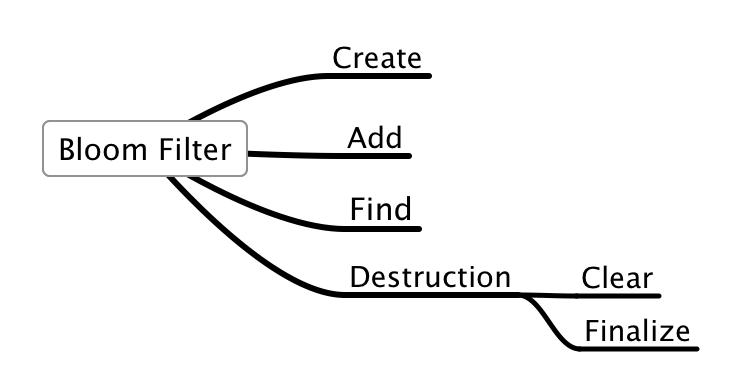
\includegraphics[scale=0.45]{BloomFilter.png}\par
\subsection{The interface: iBloomFilter}
\begin{verbatim}
typedef struct tagBloomFilterInterface {
    size_t (*CalculateSpace)(size_t maxfElements,double probability);
    BloomFilter *(*Create)(size_t maxElements,double probability);
    size_t (*Add)(BloomFilter *b,const void *key,size_t keylen);
    int (*Find)(BloomFilter *b,const void *key,size_t keylen);
    int (*Clear)(BloomFilter *b);
    int (*Finalize)(BloomFilter *b);
} BloomFilterInterface;
\end{verbatim}
\subsection{The API}
\api{CalculateSpace}
    size_t (*CalculateSpace)(size_t maxElements,double probability);
\end{verbatim}
\apidescription
Returns the space in bytes that would occupy a bloom filter to hold the given number of elements with the given probability. The probability parameter
should be greater than zero and smaller than 1.0. For values very close to the values zero and one, 
a huge number of bits can be necessary and the filter
creation function will return \Null because of lack memory problems.
\apierrors
\doerror{BADARG} The probability is smaller or equal than zero, or bigger or equal than one.
\returns
The number of bytes needed or zero in case of error.
\api{Create}
    BloomFilter *(*Create)(size_t maxElements,double probability);
\end{verbatim}
\apidescription
Creates and initializes a filter with space enough to hold \textsl{MaxElements} with the given probability for a false answer. The probability parameter
should be greater than zero and smaller than 1.0. For values very close to the values zero and one, 
a huge number of bits can be necessary and the filter
creation function will return NULL because of lack memory problems.
\apierrors
\doerror{BADARG} The probability is smaller or equal than zero, or bigger or equal than one.
\doerror{NOMEM} There is no memory for the allocation of the necessary data structures.
\returns
A pointer to a newly allocated bloom filter or \Null in case of error.
\api{Add}
    size_t (*Add)(BloomFilter *b,const void *key,size_t keylen);
\end{verbatim}
\apidescription
Adds the given key to the filter. The \texttt{keylen} argument should be the length of the key, that should never be zero.
\apierrors
\doerror{BADARG} The filter pointer or the key pointer are \Null, or the \texttt{keylen} is zero.
\doerror{CONTAINER\_FULL}. The maximum number of elements has been reached.
\returns
The number of elements in the filter or zero if there is an error.
\api{Find}
    int (*Find)(BloomFilter *b,const void *key,size_t keylen);
\end{verbatim}
\apidescription
Searches the given key in the filter.
\apierrors
\doerror{BADARG} The filter pointer or the key pointer are \Null, or the \texttt{keylen} is zero.
\returns
One if the element is found, zero if it is not, or a negative error code if an error occurs.

\api{Clear}
    int (*Clear)(BloomFilter *b);
\end{verbatim}
\apidescription
Removes all elements from the filter. No memory is released.
\apierrors
\doerror{BADARG} The given pointer is \Null.
\returns
One if all elements were cleared, a negative error code otherwise.
\api{Finalize}
    int (*Finalize)(BloomFilter *b);
\end{verbatim}
\apidescription
Releases all memory held by the filter.
\apierrors
\doerror{BADARG} The given pointer is \Null.
\returns
One if all elements were cleared, a negative error code otherwise.
%---------------------------------------------------------------------------------------------------------------------------------------
%                                             ValArray
%---------------------------------------------------------------------------------------------------------------------------------------
\newpage\section{Value arrays}
\index{iValArray}
\index{ValArray}
\renewcommand{\container}{ValArray}
Value arrays are a group of containers that store the basic types of the language: \texttt{short, int, long, long long, float, double, long double}
and have some specialized operations that should be done in hardware when the underlying CPU allows it. The objective here is to simplify the 
\texttt{vector} interface replacing the \texttt{void *} with the concrete type that these arrays hold.

We have the following ValArrays:
\begin{center}
\begin{tabular}{l|l|l}
\hline
\textbf{Name}&\textbf{Interface name}&\textbf{Element type}\\ \hline
ValArrayShort&iValArrayShort&short\\ \hline
ValArrayInt&iValArrayInt&int\\ \hline
ValArrayUInt&iValArrayUInt&unsigned\\ \hline
ValArrayLong&iValArrayLong&long\\ \hline
ValArrayDouble&iValArrayDouble&double\\ \hline
ValArrayFloat&iValArrayFloat&float\\ \hline
ValArrayLongDouble&iValArrayLongDouble&long double\\ \hline
ValArrayLLong&iValArrayLLong&long long\\ \hline
ValArrayULLong&iValArrayULLong&unsigned long long\\ \hline
ValArraySize\_t&iValArraySize\_t&size\_t\\ \hline
\end{tabular}
\end{center}
Some types can be just aliases for other types. For instance when int and long have the same size there is no point in providing a separate
implementation. This will be always the case with the type \verb,size_t, that will be an alias for one of the unsigned types. This type is needed to
represent arrays of indices that can be used to select elements into another array.

The operations supported are the same as the vector data type with several differences:
\begin{itemize}
\item Simplified interfaces. For instance in the vector container the result of GetElement is always a pointer to the data. ValArray simplifies this by
using directly the underlying type as return value. The functions that change their signature are:
\begin{enumerate}
\item Contains. Second parameter is not a pointer but the underlying type.
\item Erase. Second parameter is not a pointer but the underlying type.
\item Apply. The apply function receives the underlying type and not a pointer.
\item Add. The second argument is the underlying type.
\item GetElement. Returns the underlying type.
\item PushBack.Second argument changes.
\item PopFront. Returns the underlying type.
\item InsertAt. Second argument.
\item ReplaceAt. Third argument
\item IndexOf. Second argument.
\item Insert. Second argument
\item AddRange. Second argument is not a void pointer but a pointer to the underlying type.
\item CopyElement. Second argument is not a void pointer but a pointer to the underlying type.
\item CopyTo. The return type is not a \texttt{void **} but a pointer to an array of the underlying type.
\end{enumerate}
\item No destructors. There is no point in using destructors with the basic types.
\item No extra arguments used in the comparison function. The comparison is done inline whenever possible. The function \texttt{SetComparisonFunction}
is accepted but does nothing.
\item Creation functions do not need the element size parameter.
\item The \texttt{GetElementSize} returns the size in bytes of the underlying type but doesn't use its argument that can be \Null.
\item The \texttt{Save} and \texttt{Load} functions do not need a user defined save/load function since it is obvious how the basic
types are to be written to the disk: they contain surely no pointers that need to be followed. Their signature is changed.
\item Iterators are unchanged and still return a pointer to an element \footnote{This way it is possible to return \Null to stop the iteration of course}.
\item No tests for \Null arguments in the default version. 
Obviously those tests can be added in other versions or implementations since any \Null arguments
provokes undefined behavior \footnote{The rationale for this is that speed in these containers is very important. It is assumed that numerical software 
using this types is optimized, and a test for \Null and the corresponding jumps would slow down the number crunching.}.
\end{itemize}
\subsection{Operations}
Each operation described below needs two compatible arrays, i.e. arrays that have the same number of elements. If that is not the case an error
occurs. A single number can be used in place of an array, extending it to the shape of the array. The naming convention is to add the "Scalar" token
to the operation name, so we have for instance \texttt{MultiplyWith} and \texttt{MultiplyWithScalar}.

In general all operations use the data of the left argument and write their results into the left argument. The right argument remains unmodified.
This allows to construct efficient RPN evaluators to avoid allocating intermediate results.
\subsection{Slices and masks}
A \textbf{slice} is a description of a certain portion of the array. It has three fields:
\begin{enumerate}
\item \textbf{Start}, The zero based index of the element that starts the slice.
\item \textbf{Length}. The number of elements that are selected by the slice.
\item \textbf{Increment}. The number of elements that are skipped between elements when passing from one element of the slice to the next.
\end{enumerate}
When a ValArray is created, the slice used is the default one: \texttt{0, Size(ValArray), 1}. The slice starts at element zero,
has the same number of elements that the number of elements in the array, and its increment is 1. Using the API \texttt{SetSlice} and
\texttt{ResetSlice} you can modify the elements that will be selected for all operations. When a slice is active, all elements that aren't in the
selected slice are ignored.

Slices are maintained by the library automatically. If you erase elements from the array until the slice is empty, the library automatically
resets the slice. If you add elements, the length of the slice will increase if necessary.

A \textbf{Mask} is a boolean vector of ones or zeroes that selects elements from the array. It can be implemented as a bitstring or as a sequence
of bytes, this is implementation defined. When used in combination with some ValArray operation, it selects the elements that will be affected
by the operation.
\subsection{The interface}
This is a generic interface description. The \texttt{ElementType} token is replaced in each ValArray by the underlying type: 
int, double, etc. In the same
style, \texttt{ValArray} and the \texttt{ValArrayInterface} tokens are replaced with the corresponding value array name and interface name.
../texdoc/ValArray.tex
\pagestyle{empty}
\newpage
\hspace*{-1.0in}
\addtolength{\topmargin}{-1.8in}
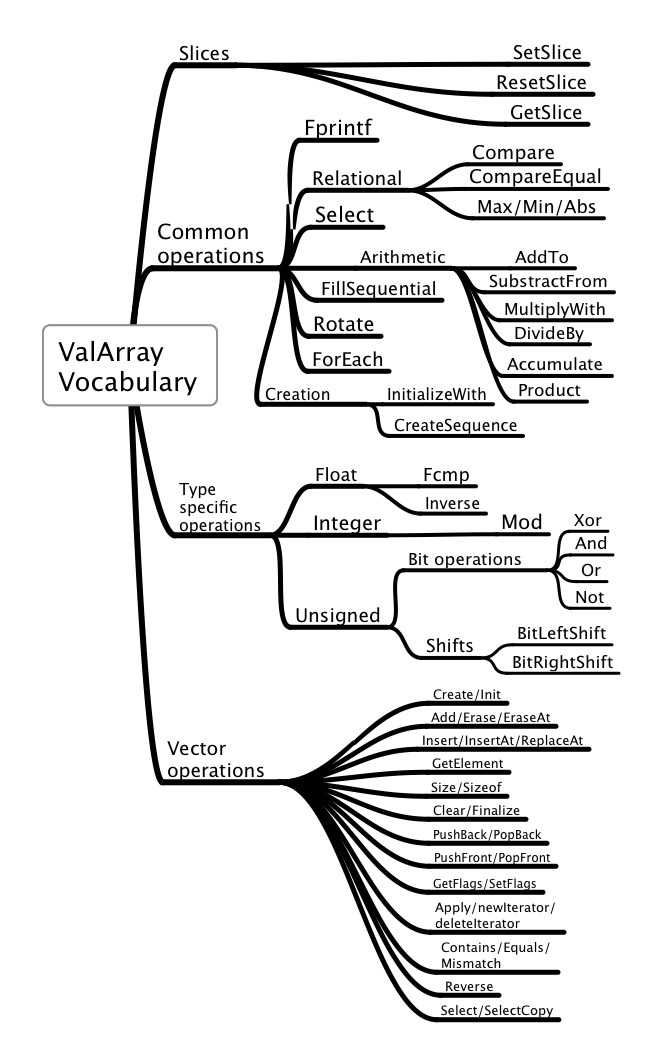
\includegraphics[scale=0.63]{ValArray.png}
\newpage
\addtolength{\topmargin}{1.8in}
\pagestyle{headings}
\api{Abs}
    int (*Abs)(ValArray *src);
\end{verbatim}
\apidescription
If any of the values in the source array is smaller than zero it will be negated. This function is only defined for signed or floating point types.
It has no meaning with unsigned types.
\returns Zero if the array was empty, a positive number if successful.
\api{Accumulate}
ElementType (*Accumulate)(ValArray *src);
\end{verbatim}
\apidescription
Calculates the sum of all the elements of the given vector. If a slice definition is active only the slice elements are considered.
\apierrors
None are mandatory but implementations should check for overflow when possible.
\returns The sum of the elements.

\api{Add}
    int (*Add)(ValArray *AL,ElementType newval);
\end{verbatim}
\apidescription
Adds an element at the end of the array. If a slice is active, the increment field (stride) will be used: the new element will be separated by the 
increment field of the slice and empty fields will be filed with zeroes. The length of the slice will be incremented by one.
\apierrors
\doerror{NOMEMORY} Not enough memory to complete the operation.
\returns
A positive number if the element was added or a negative error code otherwise.

\api{AddRange}
    int (*AddRange)(ValArray *AL,size_t n,ElementType *newvalues);
\end{verbatim}
\apidescription
Adds a range of elements at the end of the array. If a slice is active, the increment field (stride) will be used: each new element will be separated by 
the increment field of the slice and empty fields will be filed with zeroes. The length of the slice will be incremented by n. If n is zero no error
will be issued and the result is a positive number.
\apierrors
\doerror{NOMEMORY} Not enough memory to complete the operation.
\returns
A positive number if the elements were added or a negative error code otherwise.

\api{Apply}
int (*Apply)(ValArray *AL,
             int (*Applyfn)(ElementType element,void * arg),
             void *arg);
\end{verbatim}
\apidescription
Calls the given function for each element of the array. If a slice is active only the elements in the slice will be used.
\apierrors
None
\returns A positive number

\api{And}
    int (*And)(ValArray *left,ValArray *right);
\end{verbatim}
\apidescription
Performs a bitwise AND operation between each element of the right argument with the corresponding element of the left argument. Conceptually this operation is: \verb,left &= right,. This operation is allowed only between unsigned integer types. For floating point data this operation has no 
meaning. If a slice is active only the slice elements are affected. If both arrays have slices they must be compatible, i.e. they must have the
same length.
\apierrors
\doerror{INCOMPATIBLE} The arrays or slices have a different number of elements.
\returns A positive number for success, or a negative error code.

\api{BitLeftShift}
    int (*BitLeftShift)(ValArray *dst,int shift);
\end{verbatim}
\apidescription
Shifts left each element of the given ValArray by \texttt{shift} bits. If \texttt{shift} is negative it performs a right shift instead.
\apierrors
No errors. 
\returns A positive number or a negative error code if an implementation detects an invalid pointer. This error is not required to be detected.

\api{BitRightShift}
    int (*BitRightShift)(ValArray *dst,int shift);
\end{verbatim}
\apidescription
Shifts right each element of the given ValArray by \texttt{shift} bits. If \texttt{shift} is negative it performs a left shift instead.
\apierrors
No errors. 
\returns A positive number or a negative error code if an implementation detects an invalid pointer. This error is not required to be detected.

\api{Clear}
   int (*Clear)(ValArray *array);
\end{verbatim}
\apidescription
Sets the number of elements to zero but doesn't release any memory. Any slice definitions are cleared.
\apierrors
None.
\returns A positive integer.
\api{Compare}
char *(*Compare)(ValArray *left,ValArray *right,
                       char *bitarray);
\end{verbatim}
\apidescription
Assigns to each byte of the bitarray the result of comparing the corresponding elements of the left and right arrays. Conceptually this operation is: \begin{verbatim}
byte[i] = (left[i] < right[i]) ? -1 : (left[i] == right[i]) ? 0 : 1
\end{verbatim}
If the bytearray argument is \Null it will be allocated and returned. The allocator used is the one from the left argument. 
If it is not \Null it will be assumed that it contains at least
\verb,GetSize(left),
positions available.
\apierrors
\doerror{NOMEMORY}. The given byte array argument was \Null but there is no memory to allocate the result.
\doerror{INCOMPATIBLE} The arrays are of different length.
\returns A pointer to the bitarray or \Null if an error occurs.

\api{CompareScalar}
char *(*CompareScalar)(const ValArray *left,
                       const ElementType right, char *bitarray);
\end{verbatim}
\apidescription
Assigns to each byte of the bitarray the result of comparing the elements of the left array with the right argument. 
Conceptually this operation is: 
\begin{verbatim}
byte[i] = (left[i] < right) ? -1 : (left[i] == right) ? 0 : 1
\end{verbatim}
If the bitarray argument is \Null it will be allocated and returned. The allocator used is the one from the left argument. If it is not \Null it will be assumed that it contains at least
\verb,GetSize(left),
positions available.
\apierrors
\doerror{NOMEMORY}. The given byte array argument was \Null but there is no memory to allocate the result.
\returns A pointer to the bitarray or \Null if an error occurs.

\api{CompareEqual}
Mask *(*CompareEqual)(ValArray *left,ValArray *right,
                       Mask bitarray);
\end{verbatim}
\apidescription
Assigns to each element of the mask the result of comparing the corresponding elements of the left and right arrays. Conceptually this operation is: \begin{verbatim}
bit[i] = (left[i] == right[i])
\end{verbatim} 
If the bitarray argument is \Null it will be allocated and returned. The allocator used is the global memory manager. 
If it is not \Null it should contain at least enough positions to hold the data.
\apierrors
\doerror{NOMEMORY}. The given byte array argument was \Null but there is no memory to allocate the result.
\doerror{BADARG} The given mask hasn't enough positions available.
\doerror{INCOMPATIBLE} The arrays are of different length.
\returns A pointer to the bitarray passed or allocated, or \Null if an error occurs.

\api{CompareEqualScalar}
Mask *(*CompareEqual)(ValArray *left,ElementType right,
                       Mask *bitarray);
\end{verbatim}
\apidescription
Assigns to each bit of the bitarray the result of comparing the elements of the left array with the right argument. 
Conceptually this operation is: 
\begin{verbatim}
bit[i] = (left[i] == right)
\end{verbatim} 
If the bitarray argument is \Null it will be allocated and returned. The allocator used is the one from the left argument. If it is not \Null it will be assumed that it contains at least\par
\verb,1+GetSize(left)/CHAR_BIT,\par\noindent
positions available.
\apierrors
\doerror{NOMEMORY}. The given byte array argument was \Null but there is no memory to allocate the result.
\returns A pointer to the bitarray or \Null if an error occurs.

\api{Contains}
int (*Contains)(ValArray *a,ElementType data);
\end{verbatim}
\apidescription
Searches the given data in the array. If any slice specifications are active, only the slice is searched.
\apierrors
None
\returns
One if the given data is stored in the array, zero otherwise. 


\api{Copy}
    ValArray *(*Copy)(const ValArray *A);
\end{verbatim}
\apidescription
A copy of the given array is performed. The new memory will be allocated using the given array's allocator. If any slice specifications are current, 
only the elements of the slice will be copied into the resulting vector, that will have the size of the slice. Slice specifications are not copied.
\apierrors
\doerror{NOMEMORY} There is not enough memory to complete the operation.
\returns The new array. 

\api{CopyTo}
ElementType *(*CopyTo)(ValArray *AL);
\end{verbatim}
\apidescription
Copies the whole contents of the given array into a table of newly allocated elements. If a slice specification is active only the slice will be
returned.
\apierrors
\doerror{NOMEMORY} There is not enough memory to complete the operation.
\returns
A pointer to a table or \Null if an error occurs.

\api{Create}
ValArray *(*Create)(size_t capacity);
\end{verbatim}
\apidescription
Creates an empty array with enough storage to hold \texttt{capacity} elements.
\apierrors
\doerror{NOMEMORY} Not enough storage to complete this operation.
\returns A pointer to the empty array or \Null if an error occurs.

\api{CreateSequence}
ValArray *(*CreateSequence)(size_t size,
                            ElementType startValue,
                            ElementType increment);
\end{verbatim}
\apidescription
Creates an array with \texttt{size} elements and fills it with elements of the ValArray data type starting with
the \texttt{startValue} argument, and increasing it by the value of \texttt{increment} at each step. The \texttt{increment} value can be negative or zero. If it is zero the array is filled with the same value. This is equivalent to the \texttt{Fill} API\footnote{In C++ the sequence \textbf{n,0,1}
is called \textsl{iota} as in the APL language. This can be obtained with \texttt{CreateSequence(n,0,1)}}.

\apierrors
\doerror{NOMEMORY} Not enough storage to complete this operation.
\returns A pointer to the sequence or \Null if an error occurs.



\api{DivideBy}
    int (*DivideBy)(ValArray *left,ValArray *right);
\end{verbatim}
\apidescription
Divides each element of the left argument by the corresponding element of the right argument. Conceptually this operation is: \texttt{left /= right}. 
If any of the elements of the right argument is zero, an error occurs and the computation stops, leaving the left argument with some elements divided
and others not\footnote{Some implementations can provide a debug mode where the left argument is somehow preserved, or provide a mode that replaces zero by one and continues. In all cases a division by zero should provoke an error.}.
\apierrors
\doerror{INCOMPATIBLE} The arrays have a different number of elements.
\doerror{DIVIDE\_BY\_ZERO} The second argument has an element that is zero.
\returns A positive number for success, or a negative error code.

\api{DivideByScalar}
    int (*DivideByScalar)(ValArray *left, ElementType right);
\end{verbatim}
\apidescription
Divides each element of the left argument by the right argument. Conceptually this operation is: \texttt{left /= right}. If the right argument is zero
an error occurs and the left argument remains unchanged.
\apierrors
\doerror{DIVIDE\_BY\_ZERO} The second argument is zero.
\returns A positive number for success, or a negative error code.

\api{DivideScalarBy}
    int (*DivideScalarBy)(ElementType left, ValArray *right);
\end{verbatim}
\apidescription
Divides each element of the left argument by the right argument. Conceptually this operation is: \texttt{right = left / right}. If the left argument is zero
an error occurs and the right argument remains unchanged.
\apierrors
\doerror{DIVIDE\_BY\_ZERO} The first argument is zero.
\returns A positive number for success, or a negative error code.

\api{Equal}
int (*Equal)(const ValArray *src1,const ValArray *src2);
\end{verbatim}
\apidescription
Returns 1 if both arrays are equal, zero otherwise. It is legal to compare an array with \Null. If both arrays are \Null they compare equal. Any slice
definitions in the arrays must be equal. If equal, they restrict the number of elements compared. 
\apierrors
None.
\returns True or false depending if the arrays are equal or not.
\api{Erase}
    int (*Erase)(ValArray *AL,ElementType data);
\end{verbatim}
\apidescription
Removes from the vector the element that matches the given data.
\apierrors
\doerror{NOTFOUND} No match was found.
\returns
A negative error code if an error occurred, or a positive value that indicates that a match was found and the element was removed. If the element is not
in the ValArray the result value is \notfound.
%-----------------------------------------------------------------------------------------------------
\api{EraseAll}
    int (*EraseAll)(ValArray *v,const void *data);
\end{verbatim}
\apidescription
Removes from the array all elements that match the given data, that is assumed to be a pointer to an element.
\returns
A negative error code if an error occurred, or a positive value that indicates that at least a match was found and the element was removed. If the 
element is not in the list the result is \notfound.

\api{EraseAt}
    int (*EraseAt)(ValArray *AL,size_t idx);
\end{verbatim}
\apidescription
Removes from the array the element at the given position. If a slice specification is defined for the array, the index is understood as an
index within the slice and not as an index in the array.
\apierrors
\doerror{BADARG} The given vector pointer is \Null.
\doerror{INDEX} The given position is out of bounds.
\returns
A negative error code if an error occurred or a positive value that indicates that the element was removed.

\api{FCompare}
char *(*FCompare)(const ValArray *left, 
                  const ValArray *right,
                  unsigned char *bytearray, 
                  ElementType tolerance);
\end{verbatim}
\apidescription
This function is exactly like the Compare function but designed for comparing floating point numbers. Direct comparison of floating point numbers are known to be problematic. This comparison will be realized within the tolerance defined by the fourth parameter

The sample implementation uses the ideas of Donald Knuth
\footnote{ Knuth, Donald E. (1998). The Art of Computer Programming.  Volume
2: Seminumerical Algorithms. Third edition. Section 4.2.2,
p. 233. Reading, MA: Addison-Wesley.  ISBN 0-201-89684-2.}
as implemented by Theodore C. Belding
\footnote{
University of Michigan Center for the Study of Complex Systems\par
\texttt{$<$mailto:Ted.Belding@umich.edu$>$}\par
\texttt{http://www-personal.umich.edu/\textasciitilde streak}\par
}
In the documentation of its software, Mr Belding writes:
\begin{quotation}
What is needed is a comparison operator that takes into account a
certain amount of uncertainty:
\begin{verbatim}
if (fabs(x - y) <= epsilon) {
  /* code to be executed if x == y */
}

if (x - y > epsilon) {
  /* code to be executed if x > y */
}

if (x - y < -epsilon) {
  /* code to be executed if x < y */
}
\end{verbatim}
In the above code, a neighborhood is defined that extends a distance
epsilon to either side of y on the real number line.  If x falls
within epsilon of y, x is declared to be equal to y (the first case,
above).  If x is greater than y by an amount that is greater than
epsilon, x is declared to be greater than y (the second case, above).
If x is less than y by an amount that is greater than epsilon, x is
declared to be less than y (the third case, above).

The problem then becomes to determine an appropriate value of epsilon.
A fixed value of epsilon would not work for all x and y; epsilon
should be scaled larger or smaller depending on the magnitudes of the
numbers to be compared.

A floating point number is represented by two numbers, the significand
(also called the fraction or mantissa) and the exponent, and a sign,
where

\verb,0 <= significand < 1, 

and 

\texttt{number = sign * significand * pow(2, exponent)}.

Knuth's suggestion is to scale epsilon by the exponent of the larger of the
two floating point numbers to be compared:

$\Delta = epsilon \times maxExponent$

where maxExponent is the exponent of max(x, y).  Delta can then be
substituted for epsilon in the code snippets above.
\vspace{0.2cm}

{\large\textbf{Determining epsilon}}

Now that we have found a way to scale epsilon to work with a wide
range of x and y, we still need to choose an appropriate epsilon,
before scaling.  

If the number of binary digits of error, e, is known, then epsilon
can be calculated as follows:
\begin{verbatim}
epsilon = (pow(2, e) - 1) * FLT_EPSILON         (for floats)
epsilon = (pow(2, e) - 1) * DBL_EPSILON         (for doubles)
\end{verbatim}
\verb,FLT_EPSILON, and \verb,DBL_EPSILON, are equivalent to 1 ulp for single- and
double-precision numbers, respectively; they are defined in the
standard C header file \verb,<float.h>,. (An ulp is one unit in the last
place of the significand, or fraction part, of a floating point
number; see Knuth for more details.)
\end{quotation}
\apierrors
\doerror{NOMEMORY}. The given byte array argument was \Null but there is no memory to allocate the result.
\returns A pointer to the bitarray or \Null if an error occurs.

\api{FillSequential}
int (*FillSequential)(ValArray *a,
                      ElementType start,ElementType increment);
\end{verbatim}
\apidescription
Assigns to all members of the array a sequence that starts at \texttt{start}, and is incremented by the given amount at each array position.
The start and increment arguments can hold any value without restrictions, unless they go beyond the maximum value allowed for the given data
type
\apierrors
No errors. 
\returns A positive number.
\example
ValArray *myValArray = iValArray.Create(6);
iValArray.FillSequential(myValArray,5,2);
// Now the contents of myValArray are:
5,7,9,11,13,15
\end{verbatim}

\api{Finalize}
    int (*Finalize)(ValArray *AL);
\end{verbatim}
\apidescription
Reclaims all memory used by the container, including the array header object itself.
\apierrors
None
\returns
A positive value means the operation completed.

\api{ForEach}
int (*ForEach)(ValArray *src,ElementType (*ApplyFn)(ElementType));
\end{verbatim}
\apidescription
Applies the one argument \texttt{ApplyFn} to each element of the array and stores the result in that element.
\returns Always 1\footnote{The rationale for this API is to simplify the \texttt{Apply} function allowing full optimization for the compiler.
This function is used to implement all trigonometric/roots, and hyperbolic functions}.

\api{Fprintf}
int (*Fprintf)(ValArray *src,FILE *out,const char *fmt);
\end{verbatim}
\apidescription
Prints in the indicated stream each element of the given array using the indicated format string. If the array is empty nothing is printed and
the result is zero. There is a newline character appended to the output if the array wasn't empty and no error occurred.
\apierrors
\doerror{EOF} An output error occurred: impossible to write to the stream.
\returns
The number of characters written to the stream, zero if the array was empty, or a negative error code.
\api{GetCapacity}
    size_t (*GetCapacity)(const ValArray *AL);
\end{verbatim}
\apidescription
Returns the number of elements the array can hold before  it needs to reallocate its data.
\apierrors
None
\returns
The array capacity.

\api{GetData}
ElementType *(*GetData)(const ValArray *AL);
\end{verbatim}
\apidescription
Returns a pointer to the data area of the container, or \Null if an error occurs.
\apierrors
\doerror{READONLY} The container is read-only.
\doerror{BADARG} The given pointer is \Null
\returns The pointer to the array's data or \Null.

\api{GetElement}
    ElementType (*GetElement)(const ValArray *AL,size_t idx);
\end{verbatim}
\apidescription
Returns the value stored at the element with the given index.
\apierrors
\doerror{INDEX}    The given position is out of bounds.
\returns The element's value or the minimum value that can be stored in ElementType if the index is out of bounds.

\api{GetElementSize}
  size_t (*GetElementSize)(const ValArray *AL);
\end{verbatim}
\apidescription
Returns the size of the elements stored in the ValArray. The argument is not used and can be \Null.
\apierrors
None.

\api{GetRange}
    ValArray *(*GetRange)(const ValArray *AL,size_t start,size_t end);
\end{verbatim}
\apidescription
Selects a series of consecutive elements starting at position start and ending at position one less than end.
If start $>$ end or start $>$ Size(ValArray),  \Null is returned. If end is bigger than the number of elements in the array, only elements up to the number of elements will be used.\par
If a slice is active in the array, the arguments will be understood as indices in the slice and \textbf{not} in the original array.\par
The selected elements are copied into a new array. The original array remains unchanged.
\apierrors
None
\returns:
A pointer to a new ValArray containing the selected elements or \Null if an error occurs.

\api{GetSlice}
int (*GetSlice)(ValArray *array,size_t *start, size_t *length,
                 size_t *increment);
\end{verbatim}
\apidescription
Copies into the given pointers the contents of the current slice specifications for the given array. If any of the given pointers is \Null nothing is 
copied into it and no error is issued. If the array has no slice specification all fields will be set to zero if not \Null, and the result is zero.
\apierrors
No errors
\returns Zero if there isn't any slice specification, a positive number otherwise.
\example
/* This expression allows you to determine if there 
   is a slice defined for a given array */
if (iValArray.GetSlice(myValArray,NULL,NULL,NULL)) {
    /* The array has a slice defined into it */
}
\end{verbatim}

\api{IndexIn}
ValArray *(*IndexIn)(const ValArray *source,ValArraySize_t *indices);
\end{verbatim}
\apidescription
Returns an array built from indexing the first argument ("source") with the array of indexes "indices" that should be an array of 
size\_t elements. The number of elements of the resulting array is equal to the number of elements of the indexes array.
\apierrors
\doerror{INDEX} Any given position is out of bounds.
\doerror{NOMEMORY} There is not enough memory to complete the operation.
\returns
A new array or \Null if an error occurs. No partial results are returned. If any index is out of bounds the whole operation fails.

\api{IndexOf}
int (*IndexOf)(const ValArray *l,ElementType data,size_t *result);
\end{verbatim}
\apidescription
Searches for an element in the array. If found its zero based index is returned in the pointer "result". Otherwise the result of the search is \notfound. The "extraArgs" argument will be passed to the comparison function, that is used to compare elements.
\apierrors
\doerror{BADARG} The given array pointer or the element given are \Null.
\returns
A positive number if the element is found, or a negative number containing an error code or the negative constant \notfound.

\api{InitializeWith}
    ValArray *(*InitializeWith)(size_t n, ElementType *data);
\end{verbatim}
\apidescription
Creates and initializes a new ValArray with the given data table. The first argument is the number of items in the table and the second
is a pointer to a storage area that should contain at least the given number of items. 
The data is copied into the new array.
\apierrors
\doerror{NOMEMORY} There is not enough memory to complete the operation.
\returns A pointer to the new array or \Null if an error occurs.

\api{InsertAt}
    int (*InsertAt)(ValArray *src,size_t idx,ElementType newData);
\end{verbatim}
\apidescription
Inserts the new element. The new element will have the given index, that can go from zero to the vector count inclusive, i.e. one more than the number of elements in the vector.
\apierrors
\doerror{INDEX} The given position is out of bounds.
\doerror{NOMEMORY} There is not enough memory to complete the operation.

\returns
A positive value if the operation succeeded, or a negative error code if the operation failed.
\api{Inverse}
    int (*Inverse)(ValArray *src);
\end{verbatim}
\apidescription
Computes for each element the inverse (1/element) and stores it in-place. 
If a slice definition is active only their elements will be used. If any of the elements is
zero the computation stops and the result is an error code.

This function is defined for the floating point types only\footnote{For obvious reasons: using integers the inverse can have only a value of
one for the integer one, and zero for all others since we use integer division.}.
\apierrors
\doerror{DIVISION\_BY\_ZERO} One of the elements is zero.
\returns A positive number if successful, a negative error code otherwise.

\api{Max}
    ElementType (*Max)(const ValArray *src);
\end{verbatim}
\apidescription
Returns the biggest element in the container. If the container is empty it returns the smallest element that can be stored into the array's data
type\footnote{The smallest element is the identity value for the operation Max since \texttt{Max(a,smallest) ==> a} for all a}.

\api{Memset}
    int (*Memset)(ValArray *dst,ElementType data,size_t length);
\end{verbatim}
\apidescription
Assigns to each element of the argument the given data. Conceptually this operation is: \texttt{dst = data}. If a slice is active in the destination 
array only the elements described by the slice are modified. If the given length is bigger than the number of elements in the array, the array
will be expanded to accommodate the new elements.
\apierrors
\doerror{NOMEMORY} There is not enough resources to expand the array to the desired length.
\returns A positive number for success, a negative error code otherwise.


\api{Min}
    ElementType (*Min)(const ValArray *src);
\end{verbatim}
\apidescription
Returns the smallest element in the container. If the container is empty it returns the biggest element that can be stored into the array's data
type\footnote{The biggest element is the identity value for the operation Min since \texttt{Min(a,biggest) ==> a} for all a}.

\api{Mismatch}
int (*Mismatch)(const ValArray *left,const ValArray *a2,
                                         size_t *mismatch);
\end{verbatim}
\apidescription
Returns the index of the first element that is different when comparing both arrays in the passed pointer \textsl{mismatch}. If one array is shorter than the other the comparison stops
when the last element from the shorter array is compared. The comparison stops when the first difference is spotted.

If there are slice definitions in one or both arrays, they will be used.
\apierrors
None
\returns
If a mismatch is found the result is greater than zero and the \textsl{mismatch} argument will contain the index of the first element that compared
unequal. This will be always the case for arrays of different length.

If both arrays are the same length and no differences are found the result is zero and the value pointed to by the
\textsl{mismatch} argument is one more than the length of the arrays.

If an error occurs, a negative error code is returned. The \textsl{mismatch} argument contains zero.


\api{MultiplyWith}
    int (*MultiplyWith)(ValArray *left,ValArray *right);
\end{verbatim}
\apidescription
Multiplies each element of the right argument with the corresponding element of the left argument. Conceptually this operation is: \texttt{left *= right}. 
\apierrors
\doerror{INCOMPATIBLE} The arrays have a different number of elements.
\returns A positive number for success, or a negative error code.

\api{MultiplyWithScalar}
    int (*MultiplyWithScalar)(ValArray *left, ElementType right);
\end{verbatim}
\apidescription
Multiplies each element of the left argument with the right argument. Conceptually this operation is: \texttt{left *= right}. 
\apierrors
None. Some implementations could detect a bad pointer.
\returns A positive number for success, or a negative error code.


\api{Not}
    int (*Not)(ValArray *v);
\end{verbatim}
\apidescription
Performs a bitwise Not operation of each element of the argument. Conceptually this operation is: \verb,v = ~v,. This operation is allowed only between unsigned integer types. For floating point data this operation has no 
meaning. If a slice is active, only its elements will be affected.
\apierrors
\doerror{INCOMPATIBLE} The arrays have a different number of elements.
\returns A positive number for success, or a negative error code.


\api{Or}
    int (*Or)(ValArray *left,const ValArray *right);
\end{verbatim}
\apidescription
Performs a bitwise or operation between each element of the right argument with the corresponding element of the left argument. Conceptually this
operation is: \verb,left |= right,. This operation is allowed only between unsigned integer types. For floating point data this operation has no 
meaning. This operation will only affect the elements in the active slice, if a slice is active.
\apierrors
\doerror{INCOMPATIBLE} The arrays have a different number of elements.
\returns A positive number for success, or a negative error code.

\api{OrScalar}
    int (*Or)(ValArray *left,ElementType right);
\end{verbatim}
\apidescription
Performs a bitwise or operation between each element of the left argument with the right argument. Conceptually this operation is: \verb,left |= right,. This operation is allowed only between unsigned integer types. For floating point data this operation has no 
meaning.
\apierrors
\doerror{INCOMPATIBLE} The arrays have a different number of elements.
\returns A positive number for success, or a negative error code.

\api{PopBack}
int (*PopBack)(ValArray *AL,ElementType *result);
\end{verbatim}
\apidescription
Copies the last element into the given result buffer and deletes the element from the container. If the result buffer is \Null, no copy is performed.
If a slice specification is active, the element deleted will be the last element of the slice, and the length of the slice will be reduced by one.
If the slice becomes empty, the slice specifications are reset.
\apierrors
None
\returns
A negative value if an error occurs, zero if the array is empty or greater than zero if the operation succeeded.

\api{Product}
ElementType (*Product)(ValArray *src);
\end{verbatim}
\apidescription
Calculates the product of all the elements of the given vector. If a slice definition is active only the slice elements are considered.
\apierrors
None are mandatory but implementations should check for overflow when possible.
\returns The product of the elements.


\api{Reverse}
int (*Reverse)(ValArray *AL);
\end{verbatim}
\apidescription
Reverses the order of the elements of the given array.
\apierrors
\doerror{NOMEMORY} Not enough memory for intermediate storage available
\returns
A negative error code if an error occurs, or a positive value if the operation succeeded.

\api{ResetSlice}
    int (*ResetSlice)(ValArray *array);
\end{verbatim}
\apidescription Eliminates any slices specifications from the given array.
\apierrors
None.
\returns If a slice specification was removed returns 1, if no slice was defined in the given array returns zero.

\api{RotateLeft}
    int (*RotateLeft)(ValArray *src,size_t n);
\end{verbatim}
\apidescription
Rotates left the array by the indicated amount. The first n elements will be written to the end of
the array, and the rest will be shifted left to fill the empty n places.
\apierrors
None
\returns A positive number if something was moved, zero otherwise (the input was zero or a 
modulo of the array size).
\example
#include "containers.h"
int main(void)
{
        ValArrayInt * vInt = iValArrayInt.CreateSequence(24,0,1);

        printf("Original array: \n");
        iValArrayInt.Fprintf(vInt,stdout,"%d ");

        printf("Rotating left by 4\n");
        iValArrayInt.RotateLeft(vInt,4);
        iValArrayInt.Fprintf(vInt,stdout,"%d ");

        printf("Rotating left by 48\n");
        iValArrayInt.RotateLeft(vInt,48);
        iValArrayInt.Fprintf(vInt,stdout,"%d ");

        printf("Rotating left by 55\n");
        iValArrayInt.RotateLeft(vInt,55);
        iValArrayInt.Fprintf(vInt,stdout,"%d ");

        iValArrayInt.Finalize(vInt);
}

OUTPUT
Original array: 
0 1 2 3 4 5 6 7 8 9 10 11 12 13 14 15 16 17 18 19 20 21 22 23 
Rotating left by 4
4 5 6 7 8 9 10 11 12 13 14 15 16 17 18 19 20 21 22 23 0 1 2 3 
Rotating left by 48
4 5 6 7 8 9 10 11 12 13 14 15 16 17 18 19 20 21 22 23 0 1 2 3 
Rotating left by 55
11 12 13 14 15 16 17 18 19 20 21 22 23 0 1 2 3 4 5 6 7 8 9 10
\end{verbatim}
\api{RotateRight}
    int (*RotateRight)(ValArray *src,size_t n);
\end{verbatim}
\apidescription
Rotates right the array by the indicated amount. The last n elements will be written to the start of
the array, and the rest will be shifted right.
\apierrors
None
\returns A positive number if something was moved, zero otherwise (the input was zero or a 
modulo of the array size).


\api{Save}
int (*Save)(const ValArray *AL, FILE *out);
\end{verbatim}
\apidescription
The contents of the given ValArray are saved into the given stream. This function is a simplified version of the Save function in the Vector container
since it doesn't feature a save function. Since ValArrays hold primitive types they are saved in a single write into the output stream.
The output stream must be opened for writing and must be in binary mode.
\apierrors
EOF A disk input/output error occurred.

\returns
A positive value if the operation completed, a negative value or EOF otherwise.

\api{SetCompareFunction}
CompareFunction (*SetCompareFunction)(ValArray *AL,
                                         CompareFunction f);
\end{verbatim}
\apidescription
This function does nothing and returns always \Null. It is retained for compatibility purposes with other containers.
\apierrors
None
\returns Always \Null.

\api{Select}
int (*Select)(ValArray *va,Mask *m);
\end{verbatim}
\apidescription
Using the given mask, the elements where the corresponding mask element is zero are eliminated, those with a mask
value different of zero are retained. The mask must have the same length as the array.
\apierrors
\doerror{INCOMPATIBLE} The mask and the array are of different length.
\returns A positive value for success, or a negative error code otherwise.
\example
#include "containers.h"
int main(void)
{
    Mask *m = iMask.Create(18);
    ValArrayInt *va = iValArrayInt.CreateSequence(18,0,1);
    size_t i;

    for (i=0; i<18; i++) {
        iMask.Set(m,i,(i&1) ? 0 : 1);
    }
    iValArrayInt.Fprintf(va,stdout,"%3d ");
    iValArrayInt.Select(va,m);
    iValArrayInt.Fprintf(va,stdout,"%3d ");
}
OUTPUT:
0   1   2   3   4   5   6   7   8   9  10  11  12  13  14  15  16  17
0   2   4   6   8  10  12  14  16 
\end{verbatim}
\api{SelectCopy}
ValArray *(*SelectCopy)(ValArray *va,Mask *m);
\end{verbatim}
\apidescription
Using the given mask, the elements where the corresponding mask element is different from zero are copied into a new array, those with a mask
value different of zero are ignored. The mask must have the same length as the array.
\apierrors
\doerror{INCOMPATIBLE} The mask and the array are of different length.
\returns A positive value for success, or a negative error code otherwise.


\api{SetSlice}
int (*SetSlice)(ValArray *s,size_t start,
                size_t length,size_t increment);
\end{verbatim}
\apidescription
Defines a slice for the given array. The slice starts at the given index, and has \texttt{length} elements. Between each element and the next
there are \texttt{increment} positions. All operations done with the array will be done to the elements defined by the slice.

Constraints:
\begin{itemize}
\item The \texttt{start} argument can't be greater or equal than the number of elements in the array.
\item The \texttt{increment} argument must be greater than zero
\item The \texttt{length} argument must be greater than zero. If it is greater than the number of elements in the array or greater than the number of 
elements that would fit with the given increment and start it will be adjusted accordingly.
\end{itemize}
If any slice specification was defined for the given array it will be replaced by the new one.
\apierrors
\doerror{BADARG} One of the arguments doesn't meet the above constraints.
\doerror{NOMEMORY}. There is no memory to allocate the slice specifications.
\returns
Positive number if successful; negative error code otherwise.

\api{Size}
    size_t (*Size)(const ValArray *AL);
\end{verbatim}
\apidescription
Returns the total number of elements stored in the array. If there is a slice definition it will \texttt{not} be used. To know the size of a slice use the\texttt{GetSlice} API.

\api{Sizeof}
    size_t (*Sizeof)(ValArray *AL);
\end{verbatim}
\apidescription
Returns the total size in bytes of the ValArray, including the header, and all data stored in it. If the argument is \Null, the size of the header only is returned.
\returns
The number of bytes used by the vector or the size of the ValArray header if the argument is \Null.

\api{Sort}
    int (*Sort)(ValArray *AL);
\end{verbatim}
\apidescription
Sorts the given array. The order of the original array is destroyed. You should copy it if you want to preserve it. If a slice specification is active
only the elements in the slice will be sorted.
\apierrors
\doerror{NOMEMORY} Temporary storage for the operation is absent.
\returns
A positive number if sorting succeeded, a negative error code if not.


\api{SubtractFrom}
    int (*SubtractFrom)(ValArray *left,const ValArray *right);
\end{verbatim}
\apidescription
Subtracts each element of the right argument from the corresponding element of the left argument. Conceptually this operation is: \texttt{left -= right}. 
\apierrors
\doerror{INCOMPATIBLE} The arrays have a different number of elements.
\returns A positive number for success, or a negative error code.

\api{SubtractFromScalar}
    int (*SubtractFromScalar)(ElementType left,ValArray *right);
\end{verbatim}
\apidescription
Subtracts from the left argument the right argument. Conceptually this operation is: \texttt{right = left - right}. 
\apierrors
None.
\returns A positive number for success, or a negative error code.

\api{SubtractScalarFrom}
    int (*SubtractScalarFrom)(ValArray *left,ElementType right);
\end{verbatim}
\apidescription
Subtracts from the left argument the right argument. Conceptually this operation is: \texttt{left -= right}. 
\apierrors
None.
\returns A positive number for success, or a negative error code.


\api{SumTo}
    int (*SumTo)(ValArray *left,ValArray *right);
\end{verbatim}
\apidescription
Adds each element of the right argument to the corresponding element of the left argument. Conceptually this operation is: \texttt{left += right}. 
\apierrors
\doerror{INCOMPATIBLE} The arrays have a different number of elements.
\returns A positive number for success, or a negative error code.

\api{SumToScalar}
    int (*SumTo)(ValArray *left,ElementType right);
\end{verbatim}
\apidescription
Adds each element of the left argument the right argument. Conceptually this operation is: \texttt{left += right}. 
\apierrors
No errors.
\returns A positive number for success, or a negative error code.


\api{Xor}
    int (*Xor)(ValArray *left,ValArray *right);
\end{verbatim}
\apidescription
Performs a bitwise Xor operation between each element of the right argument with the corresponding element of the left argument. Conceptually this operation is: \verb,left ^= right,. This operation is allowed only between unsigned integer types. For floating point data this operation has no 
meaning.
\apierrors
\doerror{INCOMPATIBLE} The arrays have a different number of elements.
\returns A positive number for success, or a negative error code.

\api{XorScalar}
    int (*XorScalar)(ValArray *left,ElementType right);
\end{verbatim}
\apidescription
Performs a bitwise Xor operation between each element of the left argument with the right argument. Conceptually this operation is: \verb,left ^= right,. This operation is allowed only between unsigned integer types. For floating point data this operation has no 
meaning.
\apierrors
\returns A positive number for success, or a negative error code.


%---------------------------------------------------------------------------------------------------------------------------------------
%                                             Buffers
%---------------------------------------------------------------------------------------------------------------------------------------
\newpage
\section{Buffers}
\index{Buffers}
\renewcommand{\container}{Buffers}
The buffers interface is greatly simplified compared to the interface of a general container. 
The usage of a buffer as an intermediate storage means there is no sense in including all  the functionality of a container. The library provides two 
types:
\begin{enumerate}
\item Stream buffers provide linear storage that grows automatically as needed.
\item Circular buffers store the last $n$ items of a stream
\end{enumerate}
Other languages provide similar features:
\begin{itemize}
\item The Java language provides a typed buffer functionality. This buffers are not resizable, have a cursor and other more sophisticated operations 
than the buffers proposed here like slicing and compacting.Their place in the Java class hierarchy is: Object $\rightarrow$ Native I/O $\rightarrow$ 
ByteBuffer. There are methods for viewing the buffer as float, doubles, etc. 

\item The C\# language provides also a typed buffer class of the primitive types (char, float, int, etc). It is called System.Buffer and provides a few 
methods for determining its length and read/write a single byte. The language itself doesn't provide any circular buffers class but several 
implementations are available in the net. The same situation applies for Java.
\item The C++ STL doesn't provide circular buffers directly but the \texttt{boost} C++ library does provide an implementation. See:
\par
{\small
http://www.boost.org/doc/libs/1\_48\_0/libs/circular\_buffer/doc/circular\_buffer.html}
\par
In the usual simplicity of that language, the class has around 60 entry points, including specialized templates for some functions. Around 14 auxiliary 
types are involved and the documentation for this component goes for around 50 pages. That is the exact opposite of this proposal.
\end{itemize}
The design objective in this library is to keep buffers small and, while providing functionality, reduce the interface to a minimum. Compacting is not 
feasible in C due to the wide use of pointers. If there is a pointer to the data in the buffer, moving it would invalidate the pointer making for hard 
to debug crashes \footnote{Keep in mind that in circular buffers new items can overwrite old items. Do not be surprised if you keep pointers to data in 
a circular buffer, that your data changes as you add items into it}.

\subsection{Stream buffers}

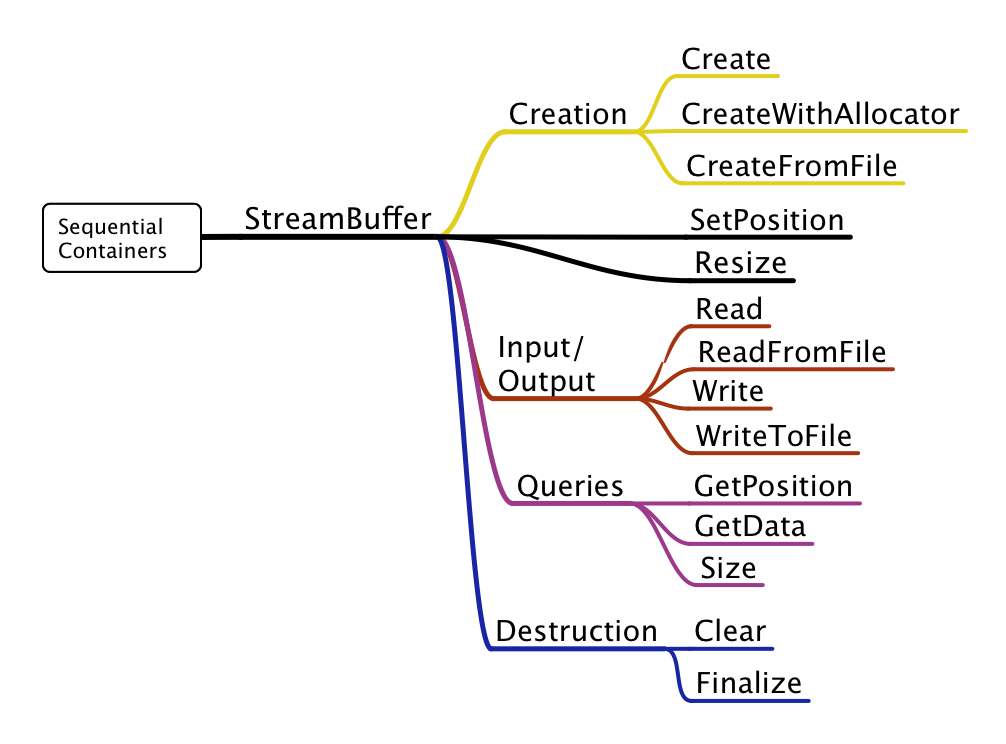
\includegraphics[scale=0.44]{StreamBuffer.png}\hfill\par

These objects are designed to store sequentially arbitrary data, resizing themselves as necessary. There is a cursor, a pointer that indicates where 
the next data item will be written. You can move the cursor, overwriting old data, or leaving holes in the buffer structure
\footnote{Buffers exist in many languages. The C++ STL doesn't explicitly provide them, but other STL extensions do, like the one proposed by 
Matthew Wilson. In that implementation, buffers store only objects of a single type. In contrast to that this library proposes no typed buffers: each buffer can store
objects of any type without any limitations, the buffer doesn't care about the type of its objects.}
.  

\subsubsection{The interface}
../texdoc/StreamBuffer.tex
\subsubsection{The API}
Noteworthy are the two functions that work with with buffers and files: \verb,ReadFromFile, and \verb,WriteToFile,. The allow you to work with a buffer when the file can't be read in one buffer, allowing
piecewise processing of portions of the file. 

The function \verb,CreateFromFile, allows you to read all the file contents into a buffer.
\api{Clear}
    int (*Clear)(StreamBuffer *b);
\end{verbatim}
\apidescription
Sets the cursor at position zero and zeroes the whole buffer.
\apierrors
\doerror{BADARG} The given buffer pointer is \Null
\returns A positive value if successful, a negative error code otherwise.

\api{Create}
    StreamBuffer *(*Create)(size_t startsize);
\end{verbatim}
\apidescription
Creates a new buffer with the given start size. If the size is zero it will use a default start value. The allocator used is the current memory manager.
\apierrors
\doerror{NOMEMORY}. There is no more memory to create the buffer.
\returns A pointer to a newly created buffer or \Null if there is no more memory left.

\api{CreateFromFile}
    StreamBuffer *(*CreateFromFile)(const char *FileName);
\end{verbatim}
\apidescription
Creates a new buffer with the contents of the given file. The allocator used is the current memory manager. The file is read in binary mode.
\apierrors
\doerror{NOMEMORY}. There is no more memory to create the buffer.
\doerror{NOENT} The file given can't be found (or it exists but the current user has no read permission).
\returns A pointer to a newly created buffer or \Null if there is no more memory left or the file can't be opened.
\api{CreateWithAllocator}
StreamBuffer *(*CreateWithAllocator)(size_t startsize, 
                                     ContainerAllocator *allocator);
\end{verbatim}
\apidescription
Creates a new buffer using the given allocator and start size. If the start size is zero a default value is used.
\apierrors
\doerror{NOMEMORY} There is no more memory to complete the operation.
\returns A pointer to the new buffer or \Null if there is no memory left.
\api{Finalize}
    int (*Finalize)(StreamBuffer *b);
\end{verbatim}
\apidescription
Releases all memory used by the buffer.
\apierrors
\doerror{BADARG} The given buffer pointer is \Null.
\returns A positive value if successful or a negative error code.
\api{GetData}
    const char *(*GetData)(const StreamBuffer *b);
\end{verbatim}
\apidescription
Returns a pointer to the data stored in the buffer. The data is read-only (const).
\apierrors
\doerror{BADARG} The given buffer pointer is \Null
\Const The given buffer is not modified. The returned pointer should not be modified.
\returns A pointer to the buffer's data or NULL, if an error occurs.

\api{GetPosition}
    size_t (*GetPosition)(const StreamBuffer *b);
\end{verbatim}
\apidescription
Returns the current cursor position.
\apierrors
\doerror{BADARG} The stream buffer pointer is \Null
\Const The stream buffer is not modified.
\returns The cursor position or zero if there is an error. Note that zero is also a valid cursor position.\footnote{Here, as in other APIs from the \texttt{buffer} interface it was preferred to have a friendly interface than to cater for errors. In case of a zero return, you should test for a \Null
pointer, but it is even better to test for it before calling this function.}
\api{Read}
    size_t (*Read)(StreamBuffer *b, void *data, size_t siz);
\end{verbatim}
\apidescription
Reads \textsl{siz} bytes from the given buffer, starting from the position of the cursor. If the buffer finishes before \textsl{siz} characters are
read, reading stops, and less characters than requested are returned. It is assumed that the \textsl{data} buffer contains at least \textsl{siz} 
characters.
\apierrors
\doerror{BADARG} Either the stream buffer, the data buffer are \Null.
\Const None. The given buffer is modified since the cursor is updated to the new position. The given buffer is modified since the data is copied 
into it.
\returns The number of characters copied or zero if there is an error. Note that if the number of requested characters is zero, this function
will also return zero.
\api{ReadFromFile}
int (*ReadFromFile)(StreamBuffer *b,FILE *f);
\end{verbatim}
\apidescription
Fills the given buffer with data from the given file. The cursor is reset to position zero.
\apierrors
\doerror{BADARG} The stream buffer pointer is \Null
\returns The number of bytes read or a negative error code.
\api{Resize}
   int (*Resize)(StreamBuffer *b,size_t newSize);
\end{verbatim}
\apidescription
Resizes the buffer to the requested size. The new size can be bigger or smaller than the current size. All pointers to the data in the buffer 
are invalid after this operation.
\apierrors
\doerror{BADARG} The stream buffer pointer is \Null.
\doerror{NOMEMORY} There is not enough memory to satisfy the request.
\returns A negative error code if an error occurs, zero if the requested size is equal to the current size, or a positive number
if the request was satisfied.
\api{SetPosition}
int (*SetPosition)(StreamBuffer *b, size_t pos);
\end{verbatim}
\apidescription
Sets the cursor at the given position. If the position is bigger than the size of the buffer the cursor is moved to the end of the buffer.

\apierrors
\doerror{BADARG} The given buffer pointer is \Null
\returns A positive value if successful, a negative error code otherwise.
\api{Size}
size_t (*Size)(const StreamBuffer *b);
\end{verbatim}
\apidescription Returns the allocated size of the buffer. If the buffer pointer is \Null returns the size of the buffer header.
\apierrors
None
\Const The given buffer is not modified.
\returns The size of the buffer.
\api{Write}
    size_t (*Write)(StreamBuffer *b,void *data, size_t siz);
\end{verbatim}
\apidescription
Writes into the buffer \textsl{siz} characters from the passed pointer \textsl{data}. The characters are written starting at the cursor
position. If the buffer is too small to hold the data, it will be enlarged using its allocator. 
\apierrors
\doerror{NOMEMORY}. There is no more memory to enlarge the buffer.
\doerror{BADARG} The stream buffer pointer or the data pointer is \Null.
\returns The number of characters written.
\example
#include <containers.h>
int main(void)
{
        StreamBuffer *sb = iStreamBuffer.Create(10);
        int i;
        char buf[20],*p;

        for (i=0; i<10; i++) {
                sprintf(buf,"item %d",i+1);
                iStreamBuffer.Write(sb,buf,1+strlen(buf));
        }
        buf[0]=0;
        iStreamBuffer.Write(sb,&buf,1);
        printf("Buffer size is: %d, position is %d\n",
                            (int)iStreamBuffer.Size(sb),
                            (int) iStreamBuffer.GetPosition(sb));
        iStreamBuffer.SetPosition(sb,0);
        p = iStreamBuffer.GetData(sb);
        while (*p) {
                printf("%s\n",p);
                p += 1 + strlen(p);
        }
        iStreamBuffer.Finalize(sb);
        return 1;
}
OUTPUT:
Buffer size is: 82, position is 72
item 1
item 2
item 3
item 4
item 5
item 6
item 7
item 8
item 9
item 10
\end{verbatim}
This example does the following:
\begin{itemize}
\item Creates a stream buffer. It assumes success and does not test the return value of the creation function. The buffer is dimensioned too small 
for the data it will contain so it has to resize several times.
\item Prepares a string buffer with sprintf and writes the resulting string including its terminating zero in the stream buffer. Note that
zeroes have no special significance in buffers. It loops ten times doing this operation.
\item It ends the buffer with a terminating double zero.
\item It prints the buffer size and the number of characters it has written. Note that they are not the same. The buffer has been resized 
several times, and at each time the new capacity is determined by an internal algorithm. Since we did not move the cursor the position of the
cursor give us the number of characters written.
\item It obtains a pointer to the data in the buffer
\item It prints all the strings in the buffer to standard output. Each character string from 1 to 9 is 7 bytes long, including its terminating zero.
The tenth string is 9 bytes, also including the terminating zero. We have then: (7*9)+9 = 72.
\item It destroys the buffer.
\end{itemize}
\api{WriteToFile}
int (*WriteToFile)(StreamBuffer *b,FILE *outfile);
\end{verbatim}
\apidescription
Writes all the contents of the given buffer to the given file. The cursor is reset to the begin of the buffer.
\apierrors
\doerror{BADARG} The stream buffer pointer or the file pointer is\Null
returns The number of bytes written.
\subsection{Circular buffers}
\includegraphics[scale=0.45]{Circular.png}\par
This objects are designed to store the last $n$ items of a stream. When they are full, the new items are stored in the same place as the oldest
item \footnote{The sample implementation allocates all the memory necessary for the container when creating it. This means that all $n\times ElementSize$ are allocated, copying the elements into it as they are added. This simplifies the management of circular buffers but is wasteful when the buffer is half empty.}. 
\subsubsection{The interface: iCircularBuffer}
\begin{verbatim}
typedef struct tagCircularBufferInterface {
    int (*Add)( CircularBuffer * b, const void *data_element);
    int (*Clear)(CircularBuffer *cb);
    CircularBuffer *(*CreateWithAllocator)(size_t sizElement,
                              size_t sizeBuffer,
                              const ContainerAllocator *allocator);
    CircularBuffer *(*Create)(size_t sizElement,size_t sizeBuffer);
    int (*Finalize)(CircularBuffer *cb);
    int (*PopFront)(CircularBuffer *b,void *result);
    int (*PeekFront)(CircularBuffer *b,void *result);
    size_t (*Size)(const CircularBuffer *cb);
    DestructorFunction SetDestructor(CircularBuffer *cb,
                                       DestructorFunction NewFn);
} CircularBufferInterface;
\end{verbatim}
\subsubsection{The API}
\api{Add}
	int (*Add)( CircularBuffer * b, const void *data_element);
\end{verbatim}
\apidescription
Adds the given data element to the circular buffer. If the buffer is full, the oldest element's place will be overwritten with the new data
and the container remains full with the same number of elements. 
\apierrors
\doerror{BADARG} One or both arguments are \Null.
\Const The given data element is not modified but copied into the container.
\returns A negative error code if an error occurs. If the container is full zero is returned. If a new element was added a positive number is returned.
\api{Clear}
	int (*Clear)(CircularBuffer *cb);
\end{verbatim}
\apidescription
Resets the number of elements inside the container to empty without freeing the memory used by the buffer.
\apierrors
\doerror{BADARG} The buffer pointer $b$ is \Null.
\returns A negative error code if an error occurs, or a positive number when the container is reset.
\api{CreateWithAllocator}
	CircularBuffer *(*CreateWithAllocator)(size_t ElementSize,
                 size_t sizeBuffer, ContainerAllocator *allocator);
\end{verbatim}
\apidescription
Creates an empty circular buffer that can hold at most $sizeBuffer$ elements, each element being of size $ElementSize$. Uses the given allocator
to allocate memory.
\apierrors
\doerror{BADARG} One or both sizes are zero, or the allocator pointer is \Null.
\doerror{NOMEM} There is no memory left.
\returns A pointer to a new circular buffer or \Null if an error occurs.
\api{Create}
	CircularBuffer *(*Create)(size_t ElementSize, size_t sizeBuffer);
\end{verbatim}
\apidescription
Creates an empty circular buffer that can hold at most $sizeBuffer$ elements, each element being of size $ElementSize$. Uses the CurrentAllocator
to allocate memory.
\apierrors
\doerror{BADARG} One or both arguments are zero.
\doerror{NOMEM} There is no memory left.
\returns A pointer to a new circular buffer or \Null if an error occurs.
\api{Finalize}
	int (*Finalize)(CircularBuffer *cb);
\end{verbatim}
\apidescription
Reclaims all memory used by the given buffer.
\apierrors
\doerror{BADARG} The buffer pointer is \Null.
\returns A positive value if the container is destroyed, a negative error code otherwise.
\api{PeekFront}
	int (*PeekFront)(CircularBuffer *b,void *result);
\end{verbatim}
\apidescription
Copies one item from the front of the circular buffer into the given buffer without removing the item from the container. 
\apierrors
\doerror{BADARG} The buffer pointer or the result buffer are \Null.
\returns A negative error code if an error occurs, zero if the buffer was empty, or a positive number if an item was copied.

\api{PopFront}
	int (*PopFront)(CircularBuffer *b,void *result);
\end{verbatim}
\apidescription
Copies one item from the front of the circular buffer into the given buffer and removes the item from the container. If the $result$ pointer is \Null
the item is removed but nothing is copied.
\apierrors
\doerror{BADARG} The buffer pointer is \Null.
\returns A negative error code if an error occurs, zero if the buffer was empty, or a positive number if an item was removed.
\example
#include <containers.h>
int main(void)
{
    CircularBuffer *cb = iCircularBuffer.Create(sizeof(int),10);
    int i,integer;

    for (i=0; i<20;i++) {
        iCircularBuffer.Add(cb,&i);
    }
    printf("There are %d elements\n",iCircularBuffer.Size(cb));
    printf("The container uses %d bytes\n",iCircularBuffer.Sizeof(cb));
    printf("The size of the header is %d\n",
                          iCircularBuffer.Sizeof(NULL));
    /* Print all elements */
    while (iCircularBuffer.PopFront(cb,&integer) > 0) {
        printf("%d ",integer);
    }
    return 0;
}
OUTPUT:
There are 10 elements
The container uses 88 bytes
The size of the header is 48
10 11 12 13 14 15 16 17 18 19
\end{verbatim}
\api{Size}
size_t (*Size)(const CircularBuffer *cb);
\end{verbatim}
\apidescription
Computes the number of items in the given circular buffer.
\apierrors
\doerror{BADARG} The buffer pointer is \Null.
\Const The given buffer is not modified.
\returns The number of items in the buffer.
\api{Sizeof}
size_t (*Sizeof)(const CircularBuffer *cb);
\end{verbatim}
\apidescription
Computes the number of bytes used by given circular buffer. If the pointer is \Null returns the size of the circular buffer header structure.
\Const the given buffer is not modified.
\returns The number of bytes used by the buffer.
%---------------------------------------------------------------------------------------------------------------------------------------
%                                             Generic
%---------------------------------------------------------------------------------------------------------------------------------------
\newpage
\section{The generic interfaces}
This interface allows the user to use containers in a generic way, ignoring its specific type.
Note that there is no "GenericContainer" object; you can't create any generic container. Once a specific container is created, it can be used as a generic container at any time since all containers comply with the generic interface. This interface just dispatches internally to the actual container and therefore incurs in a slight performance cost.
\footnote{
The Objective-C language has a similar constructs with its "Protocols". Several classes can share a common interface without any inheritance between them. Obviously in C there is no compiler support for this kind of programming, what forces your implementation to be careful about the order of the function pointers within all objects. A change in the order of those function pointers makes the object incompatible with the protocol specifications, and this can't be checked by the compiler.
All of this can be avoided, of course, if you just use the protocols designed and implemented by someone else.
}

Conceptually, the generic interfaces represent a base class (GenericContainer) and two derived classes: Sequential and Associative containers.
It would be possible to derive more classes, for instance a numeric container class that could be implemented in the future, This is left open for future releases of this specification.
\footnote{Two special cases of specialized arrays have been presented: an array of strings and an array of bits. Many other arrays are possible and surely necessary for numeric work, and they could be used as basis for vector extensions with hardware support. Another subject not mentioned in this specification  is multi-dimensional arrays.}
\subsection{Generic containers}
The general generic interface that encloses associative and sequential containers is as follows:
\index{iGenericContainer}
\begin{verbatim}
typedef struct GenericContainer GenericContainer;
typedef struct tagGenericContainerInterface {
    size_t (*Size)(const GenericContainer *Gen);
    unsigned (*GetFlags)(GenericContainer *Gen);
    unsigned (*SetFlags)(GenericContainer *Gen,unsigned flags);
    int (*Clear)(GenericContainer *Gen);
    int (*Contains)(GenericContainer *Gen,void *Value);
    int (*Erase)(GenericContainer *Gen,void *objectToDelete);
    int (*Finalize)(GenericContainer *Gen);
    void (*Apply)(GenericContainer *Gen,
                  int (*Applyfn)(void *,void * arg),
                  void *arg);
    int (*Equal)(GenericContainer *Gen1,GenericContainer *Gen2);
    GenericContainer *(*Copy)(GenericContainer *Gen);
    ErrorFunction (*SetErrorFunction)(GenericContainer *Gen,
                                      ErrorFunction fn);
    size_t (*Sizeof)(GenericContainer *Gen);
    Iterator *(*NewIterator)(GenericContainer *Gen);
    int (*deleteIterator)(Iterator *);
    int (*Save)(GenericContainer *Gen,FILE *stream, 
                SaveFunction saveFn,void *arg);
    GenericContainer *(*Load)(FILE *stream, 
                              ReadFunction readFn,void *arg);
    size_t GetElementSize(GenericContainer *Gen);
} GenericContainerInterface;
extern GenericContainerInterface iGenericContainer;
\end{verbatim}
This functions return the obvious results already described in the documentation of their container-specific counterparts and not repeated here. We only note the absence of a creation function, or any means to add an object.
\footnote{The "Erase" function  has been added to the generic interface because it has the same interface both in associative and sequential containers.The "Add" function was left out because in associative containers you need a key argument to add data. This could have been fixed by defining a structure with two fields that would be passed as a single argument, but that would make things more complex than they need to be}

Based on the generic interface, we have generic sequential and associative interfaces. They contain generic functions for adding and removing objects.
\subsection{Sequential containers}
These containers include all the functions of the GenericContainer interface, adding functions to use any sequential container as a stack, and functions for managing object replacement or addition.
\index{iSequentiaContainer}
\begin{verbatim}
typedef struct SequentialContainer SequentialContainer;
typedef struct tagSequentialContainerInterface {
    GenericContainerInterface Generic;
    int (*Add)(SequentialContainer *SC,void *Element);
    void *(*GetElement)(SequentialContainer *SC,size_t idx);
    int (*Push)(SequentialContainer *Gen,void *Element);
    int (*Pop)(SequentialContainer *Gen,void *result);
    int (*InsertAt)(SequentialContainer *SC,size_t idx, void *newval);
    int (*EraseAt)(SequentialContainer *SC,size_t idx);
    int (*ReplaceAt)(SequentialContainer *SC, 
                     size_t idx, void *element);
    int (*IndexOf)(SequentialContainer *SC,
                   void *ElementToFind,size_t *result);
    int (*Append)(SequentialContainer *SC1,SequentialContainer *SC2);
} SequentialContainerInterface;
extern SequentialContainerInterface iSequentialContainer;
\end{verbatim}
\subsection{Associative containers}
These containers include all the functions of the GenericContainer interfaces and add functions for inserting and removing objects.
\index{iAssociativeContainer}
\begin{verbatim}
typedef struct AssociativeContainer AssociativeContainer;
typedef struct tagAssociativeContainerInterface {
    GenericContainerInterface Generic;
    int (*Add)(SequentialContainer *SC,void *key,void *Element);
    void *(*GetElement)(AssociativeContainer *SC,void *Key);
    int (*Replace)(AssociativeContainer *SC, void *Key, void *element);
} AssociativeContainerInterface;
extern AssociativeContainerInterface iAssociativeContainer;
\end{verbatim} 
\chapter{Enhancing the library}
No design can ever cover all special cases that can arise during development. The advantage of the interface design is that you can enhance the library by subclassing functions that add functionality you need when absent.
Subclassing means in this context that you replace a function of the library with a new function written by you that either replaces completely the functionality of the library or that either before or after the library function adds some code that implements an enhancement.

There are several ways to enhance the library in this way:
\begin{enumerate}
\item Replace the function in the container interface object. This affects all containers of this type, including those that are already created. This involves simply assigning to the function you want to replace a new function pointer that points to a compatible function. You can save the old value and add some functionality, call the old function pointer to do what the library does, then you can add code that runs after the old library function has finished.
\item Replace the function in a copy of the functions table of a single object. This way is less intrusive than the former, since only one container is affected: the one where you modify the function table. The downside is that instead of using the simple syntax:\par\noindent \texttt{iList.Add} \par you have to use the container's table:\par \texttt{Container->VTable->Add(...)} \par This represents quite a different syntax, but this can be less of a problem if you hide it under some convenient macros \footnote{For instance you can use \texttt{iList\_Add} for \texttt{iList.Add}, or similar conventions. The specifications of the library do not define those macros to avoid invasion of the user's name space}.

On the up side, another advantage of this syntax is that you do not need to change your source code if you change the type of the container. If you write: \par \noindent \texttt{myContainer->Vtable->Add(myContainer,object);}\par \noindent this will stay the same for lists, arrays, string collections or whatever sequential container you are using. You can then change completely the type of the container just by changing the declaration.
\end{enumerate}
\section{Adding conversions between containers}
Converting one type of container into another, or creating a new container with some or all the data of an existing one are routine operations not
specified in the core library.

The reason is that there is a downside to the interface definitions as presented here: all functions within an interface module are declared 
\verb,static, to avoid polluting the user name space with those names. This has the consequence that interfaces are a monolithic  piece of
code that can't be cut in smaller pieces.

Converting an object from type "A" to another of type "B" implies then that we have \textbf{both} interfaces present. If for every container
we would define a conversion into all others, the function table of each container would need all other interfaces and if a user uses just
a single container it would need to link with the \textbf{whole} library. To avoid this problem, no conversions are specified even when surely
converting a ValArrayInt into a ValArrayDouble is an operation that will be needed sooner or later.

There are many solutions to this problem using the existing APIs:
\begin{enumerate}
\item Using a simple loop:
\begin{verbatim}
ValArrayDouble *CastToDouble(ValArrayInt *src)
{
    size_t siz = iValArrayInt.Size(src);
    ValArrayDouble *result = iValArrayDouble.Create(siz);
    size_t i;

    for (i=0; i<siz;i++) {
        double d = iValArrayInt.GetElement(src,i);
        int r = iValArrayDouble.Add(result,d);
        if (r < 0)
            break;
    }
    return result;
}
\end{verbatim}
This function stops at an error returning a partial result. Other error handling strategies could be to finalize the 
incomplete container and return \Null, or call the iError interface and then do a long jump to a recovery point, etc.
\item Using iterators:
\begin{verbatim}
ValArrayDouble *CastToDouble(ValArrayInt *src)
{
    size_t siz = iValArrayInt.Size(src);
    ValArrayDouble *result = iValArrayDouble.Create(siz);
    Iterator *it = iValArrayInt.NewIterator(src);
    int *ip;

    for (ip = it->GetFirst(src); ip;ip = it->GetNext(it)) {
        int r = iValArrayDouble.Add(result,*ip);
        if (r < 0)
            break;
    }
    iValArrayInt.DeleteIterator(it);
    return result;
}
\end{verbatim}
\item Using the Apply API.
There are surely more complex requirements for conversions. For instance we could need to extract only certain parts of the input 
container. In that case
writing a special function to be called by \verb,Apply, is justified. For instance if we have an array of structures representing customers
we could want to make a string collection with the names of all of them. 
\begin{verbatim}
// We want to extract the second field of this structure
struct customer {
    long long NumericID;
    char *Name;
    long double Balance;
};

int ApplyFn(void *data,void *container)
{
    struct customer *pData = (struct customer *)data;
    strCollection *Collection = (strCollection *)container;
    return istrCollection.Add(Collection,pData->Name);
}  

strCollection *GetAllNames(Vector *CustomerDB)
{
    size_t siz = iVector.Size(CustomerDB);
    strCollection *result = istrCollection.Create(siz);
    iVector.Apply(CustomerDB,ApplyFn,result);
    return result;
}
\end{verbatim}
\end{enumerate}
\section{Infinite arrays}
We can conceptually define an array as a function that maps an input value \textsl{index} into some output that is the \textsl{value} of the
array at that position.

In this context, an infinite array is a function that maps any member from the set of positive natural numbers  (a \verb,size_t,) into some resulting value. This function must have a value for all possible input values of its \verb,size_t, argument. For instance the function
$value=(index+5)/(index-5)$ is not usable since it would provoke a division by zero at $index=5$.

Infinite arrays exist in many computer languages.
\begin{ShorterItemize}
\item In APL they were proposed by McDonnel and Shallit in their paper "Extending APL to Infinity" \footnote{http://www.jsoftware.com/papers/eem/infinity.htm}.
\item Common lisp has the "Series" construct that is similar to infinite arrays.
\item The Translucid computer language features each variable as an infinite array of all its values
\footnote{http://cartesianprogramming.com/2012/05/22/programming-with-infinite-arrays-factorial/}
\end{ShorterItemize}

Since in the C language arrays must contain elements of the same type, obvious restrictions apply: all C types have specific bounds (defined in the
appropriate headers) so that a conceptually correct function like the Fibonacci function for instance, is not usable beyond a certain value of the
input index because of output overflow: the Fibonacci numbers grow without limit.

To implement an infinite array using the library is relatively easy. The \verb,iVector, interface has the necessary hooks for doing this.
When an index error occurs, the library calls the error function of the given vector passing it the name of the function, the integer constant 
\verb,CONTAINER_ERROR_INDEX, and a pointer to the array and the requested index. If the error function returns any other value than \Null,
the Library will assume that it is a valid pointer to some result where the real value of the array at that position is stored.

Using this information we can write this first simple implementation of an infinite array. The array function will be the \textsl{identity} function
i.e. the array will contain the value of the index at each position.
\begin{Verbatim}[numbers=left]
#include <stdarg.h>
#include <stdlib.h>
#include "containers.h"
static ErrorFunction oldErrorFn;

static void *Fn(const char *msg,int errorCode,...)
{
    va_list ap;
    size_t idx;
    static int value;
    Vector *v;
    if (errorCode != CONTAINER_ERROR_INDEX)
        return oldErrorFn(msg,errorCode);
    va_start(ap,errorCode);
    v = va_arg(ap,Vector *);
    idx = va_arg(ap,size_t);
    value = idx;
    va_end(ap);
    return &value;
}

Vector *CreateInfiniteArray(void)
{
    VectorInterface *ivct;
    Vector *result = iVector.Create(sizeof(int),1);
    if (result == NULL) return result;
    oldErrorFn = iVector.SetErrorFunction(result, Fn);
    return result;
}

int main(void)
{
    Vector *v = CreateInfiniteArray();
    int i;

    for (i=20; i<30;i++) {
        printf("%d ",*(int *)iVector.GetElement(v,i));
    }
    printf("\n");
    iVector.Finalize(v);
}

\end{Verbatim}
The central piece of the implementation is the \verb,Fn, function (lines 6 to 20) 
that will be our replacement of the default vector error function. This function
will only return something if the error is an error index (line 12). Otherwise it calls the default function stored in a static pointer.

If the error is the expected index error, we fetch the arguments (lines 15 and 16) and we set the value. 
The address of the static area is returned.

We have to write a special creation function (lines 22 to 29) that creates a vector and replaces its error function 
with our own, saving the old
value in a global variable. This value will be used if the error is not an index error.

We can now write our test program that returns 10 integers from our array. Its output is\par
\verb,20 21 22 23 24 25 26 27 28 29 ,

Note that our "infinite" array is still a perfectly valid vector object and if you use it in a "normal" way it will store the data you give it and 
return that data when you index it as any array. What it is shown in the example above is just how we can change the return value of the functions when 
an index error is detected by the library. All other uses are untouched and the vector will still behave as a normal vector.

Note also that if the error is something different than the error the software wants to modify the old procedure is called. This means that
this type of changes can be built in a cascade, each one handling only a definite type of error.

We have used here the generic interface using void pointers. Obviously we could use an integer vector instead of the generic one. To do that it would 
be necessary to change all lines that contain \verb,Vector, into \verb,intVector, and then call the \verb,iintVector.Create, function
instead of the plain \verb,iVector.Create,.

\subsection{Zero extensible arrays}
To make a zero extensible array (used in  signal processing) you would just change the line 17 above and instead of writing

\verb,value = idx;,

you would write:

\verb,value = 0;,

This type of array would return always zero for any index outside the limits of the array.
\subsection{Arrays extensible by insert}
Within the error procedure it is possible to call any function of the library. For instance, we can detect that the index error is the
result of the "InsertAt" API, and decide to enlarge the array automatically. To do this we should return a non \Null value from within  our
error procedure.

As you can see, that is \textbf{already the case}! That is why the next section is called:

\subsection{Pitfalls}
When you change the default procedure you must be careful to ensure that the \textbf{only} situations where you modify the library's behavior are
the ones you want to modify. 

\chapter{Applications}
\section{Unique}
The main point in using the C containers library is the increase in
program abstraction. In this example we will see how the library
can be used to solve in a few lines a classroom problem.

\subsubsection{Task description}
Given a text file, print in standard output the lines that are
unique in it, i.e. filtering all duplicated lines.

\subsubsection{Algorithm}
Normally this involves keeping a sorted list/array of lines
and testing if a line is in the set or  not.

\subsubsection{Solution using the CCL}
\begin{Verbatim}[numbers=left]
 #include <containers.h>
 int main(int argc,char *argv[])
 {
         FILE *f;
         int i=1,r;
         Dictionary *dict;
         char buf[8192];
         if (argc < 2) {
                 fprintf(stderr,"%s <file name>\n",argv[0]);
                 return -1;
         }
         f = fopen(argv[1],"r");
         if (f == NULL)
                 return -1;
         dict = iDictionary.Create(0,500);
         if (dict == NULL)
                 return -1;
         while (fgets(buf,sizeof(buf),f)) {
                 r= iDictionary.Add(dict,buf,NULL);
                 if (r > 0)
                         printf("[%3d] %s",i,buf);
                 else if (r < 0) break;
                 i++;
         }
         iDictionary.Finalize(dict);
         fclose(f);
 }
\end{Verbatim}
\subsubsection{Algorithm}
A hash table will be used to determine if a line is a duplicate
or not.

\subsubsection{Commentary}
We use the following local variables (lines 4-7):
\par\noindent

\begin{tabular}{l|l}
Name   & Usage\\ \hline
f      & Input stream bound to the file to read\\
i      & Counter for lines read\\
r      & Result of adding a line\\
dict   & Dictionary (Hash table)\\
buf    & Line buffer limited to 8K per line\\
\end{tabular}
\par\noindent
Lines 9-15 are concerned with opening the input file, with some error
checking.

In line 16 we create a dictionary, requesting a size of zero for the
data associated with the key since we aren't storing any data, just the
key, and we suppose that the table will contain more or less 500
entries. If the file contains much more lines performance could
suffer but the algorithm would still work.

Lines 19-25 are the main loop of the program. We read each line into
the buffer and add it to then dictionary. If the "Add" API returns
a positive number the line wasn't there, if it returns zero the
line was already in the dictionary. If the result is negative it
is an error code and we stop the loop aborting the operation. Failure
can be provoked only by lack of memory.

If the result is positive we print the line.

Cleanup is performed in lines 26 and 27: we dispose of the dictionary
and close the file.

\section{Paste}
\subsubsection{Task description}
Given two text files, print each line of them in the same line separated by a tab character. If files have a different number of lines
stop when the first file is exhausted.

Note that this specifications may be different from the Unix utility of the same name.
\subsubsection{Solution}
\begin{Verbatim}[numbers=left]
#include "containers.h"
int main(int argc,char *argv[])
{
    FILE *f1,*f2;
    char *line1,*line2;
    strCollection *file1,*file2;
    Iterator *it1,*it2;
  
    if (argc < 3) {
        fprintf(stderr,"%s: file1 file2\n",argv[0]);
        return -1;
    }
    file1 = istrCollection.CreateFromFile(argv[1]);
    file2 = istrCollection.CreateFromFile(argv[2]);
    if (file1 != NULL && file2 != NULL) {
        it1 = istrCollection.NewIterator(file1);
        it2 = istrCollection.NewIterator(file2);
        line2 = it2->GetFirst(it2); line1 = it1->GetFirst(it1);
        for (; line1; line1 = it1->GetNext(it1)) {
            if (line2) {
                printf("%s\t%s\n",line1,line2);
                line2 = it2->GetNext(it2);
            }
            else printf("%s\n",line1);
        }
        istrCollection.deleteIterator(it1);
        istrCollection.deleteIterator(it2);
    }
    istrCollection.Finalize(file1);
    istrCollection.Finalize(file2);
    return 0;
}
\end{Verbatim}
\subsubsection{Commentary}
We create two string collections containing the text (lines 13-14). Two iterators are used to get each line of both files( lines 16 17). The rest
is just cleanup: we delete the iterators (lines 26-27) and finalize the string collections (lines 29 30).

This solution using the library is shorter and easier to write than a solution reading each line with \verb,fgets(), but needs enough memory
to hold both files in memory at the same time.
\section{Mapcar}
\index{mapcar}
The lisp function "mapcar" produces a map by applying a given function to each element of a list.
\begin{verbatim}
(mapcar #'abs '(3 -4 2 -5 -6)) => (3 4 2 5 6) 
\end{verbatim}
We can reproduce this function by using "Apply". In the extra argument we pass a structure of two members: 
\begin{itemize}
\item A function to call (in the above example it would be a function to calculate the absolute value)
\item A list container where the result would be stored
\end{itemize}
Our function receives then (as all functions called by Apply) two arguments, the element and a pointer to our structure. Here is a sketch of how could it be done:
\begin{verbatim}
#include <containers.h>
struct MapcarArgs {
    void  *(*fn)(void *);
     List *Result;
};
\end{verbatim}
We keep some generality by using a general prototype and definition for the function we are using. We could have defined the callback as:
\begin{verbatim}
    int (*fn)(int *);
\end{verbatim}
That prototype would have been unusable for lists that use doubles, for instance. With the current definition we can use this "MapcarArgs" structure with any other list.

The actual function we are calling encapsulates all knowledge about the data stored in the list and the operation we perform with that data. The other parts of the software do not need to know anything about it.  It returns a static pointer to the result of the operation it performs using the given element as data that will be overwritten at each call. The intended usage is to save that result before making the next call.
It can be defined as follows:
\begin{verbatim}
void *DoAbsValue(void *element)
{
    static int result = *(int *)element;
    if (result < 0)
        result = -result;
    return &result;
}
/* This function will be directly called by "Apply". */
static int Applyfn(void *element, struct MapcarArgs *args)
{
    void *result = args->fn(element);
    int r = iList.Add(args->Result,result);
    return r;
}
List *mapcar(List *li,void *(*fn)(void *))
{
        struct MapcarArgs args;

        args.fn = fn;
        args.Result = iList.Create(iList.GetElementSize(li));
        if (args.Result == NULL)
                return NULL;
        iList.Apply(li,Applyfn,(void *)&args);
        return args.Result;
}

int main(void)
{
    List *li = iList.Create(sizeof(int));
    List *newList;
    int i;
    int tab[] = {3,-4,2,-5,6};
    for (i=0; i<5;i++) {
        iList.Add(li,&tab[i]);
    }
    newList = mapcar(li,DoAbsValue);
}
\end{verbatim}
Still, our version of mapcar is still specific to lists. A more general version would use a sequential container to make a mapcar function that would be able to work with any type of sequential container. 

The basic idea is to provide an empty container of the desired result type as an extra argument to mapcar. We use an iterator instead of "Apply", obtaining a single compact function that will take any sequential container as input an add the result of the function to any type of sequential container.
\begin{verbatim}
int mapcar(SequentialContainer *src,         /* The source container */
           void *(*fn)(void *),/* Function to call with each element */
           SequentialContainer *result)   /* The resulting container */
{
        Iterator *it = iSequentialContainer.NewIterator(src);
        int r=1;
        void *obj;
        if (it == NULL)
               return CONTAINER_ERROR_NOMEMORY;
        for (obj = it->GetFirst(it);
              obj != NULL;
              obj = it->GetNext(it)) {
              void *tmp = fn(obj);
              int r = iSequentialContainer.Add(result,tmp);
              if (r < 0) {
                    /* In case of any error return a partial result 
                    and the error code */
                    break;
               }
        }
        deleteIterator(it);
        return r;
}
\end{verbatim}
Other similar functions can be built from this model. For instance "mapcon", a function that needs two containers to build a resulting container. The result is  made out of the results of a binary function that will receive one element from each container. 

Its implementation is trivially deduced from the above function:
\index{mapcon}
\begin{verbatim}
int mapcon(SequentialContainer *src1,
           SequentialContainer *src2,  /* The input containers */
           void *(*fn)(void *,void *),  /* Function with 2 arguments */
           SequentialContainer *result)   /* The resulting container */
{
        Iterator *it1 = iSequentialContainer.NewIterator(src1);
        Iterator *it2 = iSequentialContainer.NewIterator(src2);
        int r=1;
        void *obj1,*obj2;
        if (it == NULL)
               return CONTAINER_ERROR_NOMEMORY;
        if (iSequentialContainer.GetElementSize(src1) != 
            iSequentialContainer.GetElementSize(src2)) {
            return CONTAINER_ERROR_INCOMPATIBLE;
        }
        for (obj1 = it1->GetFirst(it1),obj2 = it2->GetFirst(it2);
              obj1 != NULL && obj2 != NULL;
              obj2 = it2->GetNext(it2),
              obj1 = it1->GetNext(it1)) {
              void *tmp = fn(obj1,obj2);
              int r = iSequentialContainer.Add(result,tmp);
              if (r < 0) {
                    /* In case of any error return a partial result 
                    and the error code */
                    break;
               }
        }
        deleteIterator(it1);
        deleteIterator(it2);
        return r;
}
\end{verbatim}
We can use it with a function  that adds its two arguments to add two containers:
\begin{verbatim}
void *DoAdd(void *element1,void *element2)
{
    static int result = *(int *)element1 + *(int *)element2;
    return &result;
}
\end{verbatim}
Note that not all errors are detected, and we stop at the smallest container, producing a result compatible with the smallest of both arguments.
Note too that we make a very superficial compatibility test to see if the arguments contain the same type of object, using their size as an indication. This test would ignore elements of the same size but incompatible, for instance floats and 32 bit integers, or 64 bit integers and double precision elements, etc.

The standard answer to the above problems is to point out that C has a tradition of keeping things simple and expecting programmers that take care of low level details. If you want more error support, you will find out with minimal research a lot of languages ready to make all kinds of hand holding for you.


%--------------------------------------------------------------------------------------------------------------
%                                                The sample implementation
%-------------------------------------------------------------------------------------------------------------
\chapter{The sample implementation}
The objective of the sample implementation is to serve as a guide for the implementors of this proposal. It is not the fastest implementation and it is not the most efficient or compact one. As any other software, it contains bugs, that I hope to iron out with time.

Please note that all the decisions done for the sample implementation are \textbf{not} part of the specifications of the containers library. Other
implementations could do completely different things\footnote{The full source code of the sample implementation can be downloaded from
the project's home page  \Verb,http://code.google.com/p/ccl/,. There you can find also the source code of this documentation. }.
\section{The different source files}

The sample implementation has two types of files:
\begin{enumerate}
\item Source files that implement a specific container: list.c vector.c, etc. This containers use a void pointer to receive their arguments and return
a void pointer when retrieving their data.
\item Source files that implement a \textsl{templated} container, i.e. the file needs a \textsl{parameter file} and a \textsl{templated implementation} 
file. In this type of files we have a small file that defines the templated file parameters (in the form of pre-processor macros) and then just 
includes the templated implementation file. This containers receive data of a concrete type passed by value and return the same data passed by value.
\end{enumerate}

{\small
\begin{longtable}{||p{3.5cm}|p{11cm}||}
\hline
\textbf{File}&\textbf{Description}\\\hline \hline 
bitstrings.c&The bitstring container.\\\hline
bloom.c&The bloom filter container\\\hline
buffer.c&Growable buffers and circular buffers\\\hline
ccl\_internal.h&Definitions of all the types defined internally by the library.\\\hline
containers.h&Main header file of the library. It defines all the user visible interfaces.\\\hline
deque.c&The deque container\\\hline
dlistgen.h&Generic definition of the double linked list data-type specific containers.\\\hline
dictionary.c&Hash tables using ASCII text as key. This is just a small file that sets the parameters for the \verb,dictionarygen.c, file\\\hline
dictionarygen.c&Common code for the dictionary container using either ASCII or wide characters keys\\\hline
dlist.c&Double linked list container using void pointers to store the data.\\\hline
dlistgen.c&Double linked list container using a specific data type. Needs a parameter file\\\hline
dlistgen.h&Double linked list container data definitions and interface definitions using a specific data type. Needs a parameter file\\\hline
doubledlist.c&Double linked list for double data. This is a parameter file for dlistgen.c\\\hline
doubledlist.h&Single linked list header file for double data. This is a parameter file for dlistgen.h\\\hline
doublelist.c& Parameter file for listgen.c producing the doubleList container\\\hline
doublelist.h&Parameter file for listgen.h for doubleList container\\\hline
error.c&The error interface\\\hline
fgetline.c&Reads a line of text from a file. Used in the string container\\\hline
generic.c&The generic container interface\\\hline
hashtable.c&Hash table featuring binary keys\\\hline
heap.c&Small object allocator\\\hline
iMask.c&Mask interface implementation\\\hline
intdlist.c&Parameter file for dlistgen.c defining the intDlist container\\\hline
intdlist.h&Parameter header for dlistgen.h declaring intDlist container\\\hline
intlist.c&Parameter file for listgen.c defining intList container\\\hline
intlist.h&Parameter header for listgen.h declaring intList container\\\hline
list.c&Generic type list container using void pointers\\\hline
listgen.c&Template file for List container\\\hline
longlongdlist.c&Parameter file for dlistgen.c defining longlongDlist container.\\\hline
longlonglist.c&Parameter file for listgen.c\\\hline
malloc\_debug.c&Debug implementation of malloc\\\hline
Makefile&Make file for Unix systems using the gcc compiler\\\hline
Makefile.lcc&Make file for windows systems using the 32 bit lcc compiler\\\hline
Makefile.lcc64&Make file for windows systems using the 64 bit lcc compiler\\\hline
Makefile.msvc&Make file for windows systems using the Microsoft compiler\\\hline
memoryanager.c&Very short file describing the CurrentAllocator mechanism.\\\hline
observer.c&The implementation of the observer pattern\\\hline
pool.c&Pooled memory manager\\\hline
pooldebug.c&Debug version of the pool memory manager\\\hline
priorityqueue.c&Priority queues implementation\\\hline
qsortex.c&Quick sort algorithm\\\hline
queue.c&Queue container\\\hline
redblacktree.c&Red black tree implementation. Not yet documented\\\hline
scapegoat.c&"Scapegoat" trees implementation\\\hline
searchtree.c&AVL trees. Not documented\\\hline
sequential.c&Implementation of the general sequential container interface\\\hline
smallpool.c&Not documented yet\\\hline
strcollection.c&Specialized vector for ascii character strings. This is a parameter file for strcollectiongen.c.\\\hline
stringlist.c&Specialized version of single linked lists using strings\\\hline
stringlistgen.c&Common code for ascii and wide character strings specialized vector\\\hline
valarraydouble.c&Value array of double data. Parameter file for valarraygen.c\\\hline
valarrayfloat.c&Value array of float data. Parameter file for valarraygen.c\\\hline
valarrayint.c&Value array of int data. Parameter file for valarraygen.c\\\hline
valarraylongdouble.c&Value array of long double data. Parameter file for valarraygen.c\\\hline
valarraylonglong.c&Value array of long long data. Parameter file for valarraygen.c\\\hline
valarrayshort.c&Value array of short data. Parameter file for valarraygen.c\\\hline
valarraysize\_t.c&Value array of size\_t data. Parameter file for valarraygen.c\\\hline
valarrayuint.c&Value array of unsigned int data. Parameter file for valarraygen.c\\\hline
valarrayulonglong.c&Value array of unsigned long long data. Parameter file for valarraygen.c\\\hline
valarraygen.c&Common code for all val array implementations.\\\hline
valarraygen.h&Common header file for all val array implementations. Needs a parameter file\\\hline
vector.c&Code for the vector container\\\hline
vectorgen.h&Header file for the template form of the vector container\\\hline
vectorgen.c&Implementation of the template form of the vector container\\\hline
wdictionary.c&Dictionary for a dictionary using wide character strings\\\hline
wstrcollection.c&String collection using wide character data. Parameter file for strcollectiongen.c\\\hline \hline
\end{longtable}
} % End of scriptsize
\subsection{Building the software}
The library comes with several "makefiles" to build it automatically. Those makefiles build a library called \verb,libccl.a, under Unix systems, or \verb,ccl.lib, under windows.
\begin{ShorterItemize}
\item Type \verb,make, for building the files under Unix
\item Type \verb,make -f Makefile.lcc, for building under windows 32 bit with the lcc compiler
\item Type \verb,make -f Makefile.lcc64, for building under windows 64 bit with the lcc64 compiler
\item Type \verb,nmake -f Makefile.msvc, for building under windows with the Microsoft MSVC compiler
\end{ShorterItemize}
\section{Partitioning}
An interface is a table of functions. This tables are a monolithic construct: if you use only one of the functions of the
interface you will have to link with all of the interface functions, whether you use them or not.

It is important then, that each interface doesn't "pull in" other interfaces since then you would end up linking with the whole library even if
you use a small fraction of it.

Some of this is inevitable though. All interfaces use the observer interface, so if you use any interface the observer interface will be
pulled in. It is important then, that the dependencies of the observer interface be kept to a minimum 
\footnote{Early versions of the library used the vector interface to maintain the association between an object and its callbacks. That meant that the vector interface would be pulled in too. And since the vector interface uses the heap interface object, that one would be pulled in also.}. Problem is, it is necessary for the
observer interface to set the flags of the container being registered as an observed object. This means that the generic interface is needed.

Go avoid pulling in the whole generic interface, the observer functions use the \texttt{vTable}. In the sample implementation all containers
have a table of functions as first interface field. Since the description of the generic container object is published in "containers.h" it can
use the generic notation.
\begin{verbatim}
GenericContainer *gen = (GenericContainer *)InputObject;
unsigned flags = gen->vTable->GetFlags(gen);
\end{verbatim}

This works because the sample implementation has carefully designed all interface to be binary compatible, allowing an easy implementation
of the generic interface. All vTables have the \texttt{GetFlags} function at the same place, so we always call the correct function.

Another interface that is used by all other interfaces is the error interface. It has been kept as small as possible to avoid pulling in too much
data into the fixed overhead.

\section{Data structures}
All container data structures are composed of two parts:
\begin{enumerate}
\item A header part, containing a pointer to the functions table and some other fields. This 'generic' part is at the start of all container header structures.
\item A container specific part, containing auxiliary structures and data needed for the specific container at hand.
\end{enumerate}
\subsection{The generic part}
The first part of all container data structures is the same for each container. This allows to implement conceptually an abstract class of objects: the 'generic' container.
\index{Generic Container!structure}
\begin{verbatim}
struct GenericContainer {
    GenericContainerInterface *vTable;
    size_t Size;
    unsigned Flags;
    size_t ElementSize;
};
\end{verbatim}
\begin{enumerate}
\item \texttt{Vtable}. All containers in the sample implementation contain a pointer to the table of functions of their interface.
\item \texttt{Size}. The number of elements this container stores.
\item \texttt{Flags}. Stores the state of the container. The only flag the sample implementation uses is the \texttt{READ\_ONLY\_FLAG} but many others 
are possible, for instance a 'locked' flag for multi-threading access, or a 'copy on write' flag for lazy copy, etc.
\item \texttt{ElementSize}. All containers in the sample implementation can store objects of the same size. This is not really a limitation since you 
can store objects of ANY size by storing a pointer in the container.
An alternative design would store objects of any size but it would need to store the size of each object in addition to the data used by the object. 
The specialized containers like bitstrings, string collections or integer/double arrays do not need this field obviously, and its presence is optional.
\end{enumerate}
\subsection{Lists}
\includegraphics[scale=0.63]{List.png}

Single linked lists use a single pointer to the next element. The data for the element comes right behind that pointer to avoid the overhead that yet 
another pointer would represent.
\begin{verbatim}
typedef struct _list_element {
    struct _list_element *Next;
    char Data[MINIMUM_ARRAY_INDEX];     // See below
} list_element;
\end{verbatim}
The list header uses this structure to store the elements\footnote{The constant \texttt{MINIMUM\_ARRAY\_INDEX} is defined as 1 if we are compiling in 
C90 mode or as nothing if we are compiling in C99 mode. In C99 mode we have a flexible structure, that consists of a fixed and a variable part. The 
fixed part is the pointer to the next element. The variable part is the object we are storing in the list. 
}. As you can see, there is no space wasted in a pointer to the element stored. The element stored is placed just behind the \texttt{Next} pointer. The 
downside of this decision is that we can't recycle this object to store other different objects of different size.
\subsection{Source files}
\begin{center}
\includegraphics[scale=0.41]{ListContainerSourceFiles.png}
\end{center}

The figure shows the files associated with the two implementations of the list container. The generic pointers implementation is \verb,list.c, and the 
\textsl{templated} implementation is in \verb,listgen.c,. The files depending on \verb,listgen.c, are \textsl{parameter} files for \verb,listgen.c,.
\subsubsection{Alignment}
Some machines require that data be stored at particular addresses, always a multiple of two. For instance SPARC machines require that doubles be
aligned at a multiple of 8. The structure for our list element above would provoke a crash when used to store doubles
\footnote{Modern versions of the operating systems that use SPARC catch the exception, load the data with several instructions and return control
to the program transparently. This wasn't the case in the older versions, and anyway the SPARC example is an example for a whole class of machines
that require alignment.}. 

In those machines the list element structure is defined as follows:
\begin{verbatim}
typedef struct _ListElement {
    struct _ListElement *Next;
#ifdef SPARC32
    void *alignment;
#endif
    char Data[MINIMUM_ARRAY_INDEX];
} ListElement;
\end{verbatim}

This assumes that \verb,sizeof(void *), is 4. 

In machines that handle unaligned data gracefully without crashing alignment requirements aren't useless, since in most cases they 
provoke a performance loss.
\index{lists!structure}
\begin{verbatim}
struct _List {
    ListInterface *VTable;  
    size_t count;           
    unsigned Flags;	
    unsigned timestamp;   
    size_t ElementSize;   
    list_element *Last;   
    list_element *First;  
    CompareFunction Compare; 
    ErrorFunction RaiseError; 
    ContainerHeap *Heap;
    ContainerAllocator *Allocator;
};
\end{verbatim}
In the public \texttt{containers.h} header file we refer always to an abstract structure \texttt{\_List}. We define it here. This schema allows other 
implementation to use the same header with maybe radically different implementations of their data structure.
\begin{enumerate}
\item \texttt{Vtable}, \texttt{count}, \texttt{Flags}, \texttt{ElementSize}. This fields were described in the generic container section.
\item \texttt{timestamp}. This field is incremented at each modification of the list, and allows the iterators to detect if the container changes 
during an iteration: they store the value of this field at the start of the iteration, and before each iteration they compare it with its current 
value. If there are any changes, they return \Null.
\item \texttt{Last}. Stores a pointer to the last element of the list. This allows the addition of an element at the end of the list to be fast, 
avoiding a complete rescan of the list. This field is an optimization, all algorithms of a single linked list would work without this field.
\item \texttt{First}. The start of the linked list.
\item \texttt{Compare}. A comparison function for the type of elements stored in the list.
\item \texttt{RaiseError}. A function that will be called when an error occurs. This field is necessary only if you want to keep the flexibility of 
having a different error function for each list that the client software builds. An alternative implementation would store a pointer to an error 
function in the interface.
\item \texttt{Allocator}. A set of functions that allocates memory for this list. In an implementation that needs less flexibility and is more 
interested in saving space it could be replaced by the default allocator.
\end{enumerate}
The sample implementation has certainly a quite voluminous header because of a design decision to keep things very flexible. Other implementations 
could trim most of the fields, and an absolute minimal implementation would trim \texttt{Last}, \texttt{Compare}, \texttt{RaiseError}, \texttt{Heap}, 
and \texttt{Allocator}. If the implementation assumes that only one iterator per container is allowed, the \texttt{timestamp} field could be replace by 
a single bit ('changed') in the \texttt{Flags} field.\footnote{The function \texttt{newContainer} would clear the 'changed' bit, and the iterator 
functions would test if it is still clear. All modifications function would set it to one. This simple schema becomes problematic when you consider 
what happens when an invalid iterator is used again. In the simple one bit schema if the flag has been cleared, the iterator goes on, in the more 
expensive schema of the sample  implementation, the stalled iterators are never restartable until the counter wraps around to the same value.}
\subsection{Double linked lists}
This container has a very similar structure to the single linked ones
\begin{verbatim}
typedef struct _dlist_element {
    struct _dlist_element *Next;
	struct _dlist_element *Previous;
    char Data[MINIMUM_ARRAY_INDEX];   /* (1) */
} dlist_element;
\end{verbatim}

(1): In the \textsl{templated} versions of the container this field is defined as: \verb,TYPE Data;, where \verb,TYPE, is a type 
definition passed to the file as a parameter.

We have now two pointers followed by the stored data. All other fields are exactly identical to the ones in the single linked list. The single 
difference is the existence of a free list. This could have been done in the single linked list implementation too.
\index{Dlist!structure definition}
\begin{verbatim}
struct Dlist {
    DlistInterface *VTable;
    size_t count;        
    unsigned Flags;
    unsigned timestamp;
    size_t ElementSize;
    dlist_element *Last; 
    dlist_element *First;
    dlist_element *FreeList;
    CompareFunction Compare;
    ErrorFunction RaiseError; 
    ContainerHeap *Heap;
    ContainerAllocator *Allocator;
};
\end{verbatim}

\subsection{Vector}
Arrays are the containers that use the smallest overhead per element: zero. The only overhead is the header structure, whose cost is amortized since it is fixed for all elements that the array can hold.

This is a 'flexible' array however, what means that there is some spare space allocated for allowing further growth, and that different allocation strategies can be followed when allocating a new chunk of array space when the existing array is full.
\index{Vector!structure}
\begin{verbatim}
struct _Vector {
    VectorInterface *VTable;
    size_t count;          
    unsigned int Flags;    
    size_t ElementSize;	
    void *contents;        
    size_t capacity;       
    unsigned timestamp;
    CompareFunction CompareFn;
    ErrorFunction RaiseError;
    ContainerAllocator *Allocator;
} ;
\end{verbatim}
\begin{enumerate}
\item \texttt{Vtable}, \texttt{count}, \texttt{Flags}, \texttt{ElementSize}. This fields were described in the generic container section.
\item \texttt{CompareFn, RaiseError, timestamp} and \texttt{Allocator} were described in the \texttt{List} container.
\item \texttt{capacity}. Stores the number of elements (of \verb,ElementSize, bytes each) this container can hold without resizing.
\item \texttt{contents}. Points to an array of \texttt{capacity} elements, each of size \texttt{ElementSize}.
\end{enumerate}
\subsection{Dictionary}
This container consists of an array of single linked lists. It could have been done with an \texttt{Vector} of \texttt{List} containers but a dedicated implementation is justified because of a greater efficiency. The advantages of the \texttt{Vector} container (secured access, flexible expansion) are not needed since the array has a fixed length that never changes.
\index{Dictionary!structure definition}
\begin{verbatim}
struct _Dictionary {
    DictionaryInterface *VTable;
    size_t count;
    unsigned Flags;
    size_t size;
    ErrorFunction RaiseError;
    unsigned timestamp;
    size_t ElementSize;
    ContainerAllocator *Allocator;
    unsigned (*hash)(const char *Key);
    struct DataList {
        struct DataList *Next;
        char *Key;     /* (1) */
        char *Value;
    } **buckets;
};
\end{verbatim}

(1): In the wide character version of this structure, this field will be defined as: \verb,wchar_t *Key;,\par
\begin{enumerate}
\item \texttt{Vtable}, \texttt{count}, \texttt{Flags}, \texttt{ElementSize}. This fields were described in the generic container section.
\item \texttt{RaiseError, timestamp} and \texttt{Allocator} were described in the \texttt{List} container.
\item \texttt{size}. The number of different lists that the hash table can contain. This is normally a prime number.
\item \texttt{hash}. A hash function for character strings.
\item \texttt{buckets}. A table of pointers to lists of \texttt{DataList} structures.
\end{enumerate}
\subsection{String collection}
String collections are just flexible arrays of pointers to C character strings. They share all the fields of the Vector container, the only specific 
field is a context that is passed to the string comparison function. This context can contain flags or other information to use with special text 
encodings (wide characters for instance) or other data like regular expressions, etc.
\index{strCollection!structure}
\begin{verbatim}
struct strCollection {
    strCollectionInterface *VTable;
    size_t count; 
    unsigned int Flags;
    char **contents;      /* (1) */
    size_t capacity;
    size_t timestamp;
    ErrorFunction RaiseError;
    StringCompareFn strcompare;
    CompareInfo *StringCompareContext;
    ContainerAllocator *Allocator;
};
\end{verbatim}
(1): In the wide character version of this structure this field is defined as:
\begin{verbatim}
    wchar_t ** contents;
\end{verbatim}
\subsection{Masks}
There were two alternatives for implementing masks: 
\index{Mask!structure definition}
\begin{ShorterItemize}
\item Bit strings. Each bit position can hold a boolean value.
\item A character array. Each position can hold more values, for instance -1, 0, and 1, to hold the results of comparisons. This solution was retained
for the sample implementation. Item access is simplified and faster, at the expense of course of more memory.
\end{ShorterItemize}
\begin{verbatim}
struct _Mask {
    size_t length;
    const ContainerAllocator *Allocator;
    char data[];
};
\end{verbatim}
\subsection{Bit strings}
Bit strings do not need the ElementSize field obviously. The \verb,BIT_TYPE, macro is defined as unsigned char. In general it should be an
unsigned integer type that could be different from char, maybe a 32 bit type or even larger.
\index{BitString!structure definition}
\begin{verbatim}
struct _BitString {
    BitStringInterface *VTable; /* The table of functions */
    size_t count;         /* number of bits in the array */
    BIT_TYPE *contents;   /* The contents of the collection */
    size_t capacity;      /* allocated space in the contents vector */
    unsigned timestamp;   /* Modifications counter */
    unsigned int Flags;   /* Read-only or other flags */
    const ContainerAllocator *Allocator;
} ;
\end{verbatim}

\subsection{The iterator implementation}
This data structure has two main parts:
\begin{itemize}
\item A public part:
\index{Iterator!structure}
\begin{verbatim}
typedef struct _Iterator {
    void *(*GetNext)(struct _Iterator *);
    void *(*GetPrevious)(struct _Iterator *);
    void *(*GetFirst)(struct _Iterator *);
    void *(*GetCurrent)(struct _Iterator *);
    void *(*GetLast)(struct _Iterator *);
    void *(*Seek)(struct _Iterator *,size_t);
    int   (*Replace)(struct _Iterator *,void *data,int direction);
} Iterator;
\end{verbatim} 
This part contains only the functions that the interface offers. It is defined in the public header \verb,containers.h,.
\item A private, container specific part that comes right behind the public part and stores additional information that is needed for each container. 
For instance the list container will add following fields:
\index{ListIterator}
\begin{verbatim}
struct ListIterator {
    Iterator it;          // Includes the public part
    List *L;              // List this iterator is going through
    size_t index;         // The position where we are in the list
    list_element *Current;// The current element
    size_t timestamp;     // The timestamp of the list when this
                          // iterator was created
    char ElementBuffer[1];// The current element if needed
};
\end{verbatim}
User code should only see and use the public part, as if the iterator was only the public part. Internally all iterator functions are completely 
different functions, specific for the container they should iterate. It looks like from user code, as you were always calling the same function because 
the syntax and name is the same. This allows for a certain abstraction in the source code that uses this functions, allowing to express a whole range 
of algorithms in terms of general concepts.

Each of the functions that implement \texttt{GetNext} \texttt{GetFirst}, etc starts with a cast of the input argument that is declared as an 
\texttt{Iterator} structure to a concrete container iterator like our \texttt{ListIterator} above.

In all those structures there is a common ground. They have:
\begin{enumerate}
\item A pointer to the container the iterator is using.
\item Some fields for storing the current position within the container, i.e. a cursor.
\item A \texttt{timestamp} field to detect if the container has changed during the iteration.
\item A buffer that allows the iterator to store an element of the container. This area contains a copy of the current element. Normally the
iterators return a pointer to the data of each element, but in the case of read only containers a pointer to this area will be returned. 
This allows to maintain the read only semantics.
\end{enumerate}
\end{itemize}
\subsection{The timestamp field}
This field will be incremented by each modification of the list. When an iterator is created it will copy the current value of the time stamp, and for
each subsequent operation it will compare the value of the container with its saved copy. They should be always equal, otherwise the iterator will
return always \Null. The only exception to this rule is the iterator \verb,Replace, function that will modify the container without invalidating
the iterator that calls it. Other iterators to the same container will be invalidated.

The timestamp field should be incremented in all operations that somehow modify the container, not only in the operations that modify the number of 
elements.
\notes{Implementation issues}
\begin{itemize}
\item
There is currently no way to know when you delete a container if there are iterators that are still
pointing to it. This could be detected by simply having a counter of the number of iterators a container has, but that would mean more overhead for the 
already fat header objects...
\item The current interface requires that the user calls the \verb,deleteIterator, function when you are done using the iterator. This is
a source of memory leaks if you forget
to do it. An easier way to do this would be to maintain a list of current iterators, to be freed automatically when the container is 
destroyed. Obviously this supposes that you do not create thousands of iterators but that you reuse the iterators for different loops.
\end{itemize}
\section{The code}
Only one container will be shown here in full: the List container. For the others, only some functions will be explained to save space. You are 
invited to read the distributed code of course that is part of this work.
\subsection{List}

\index{lists!code}
\renewcommand{\container}{list}
\function{Add}
static int Add_nd(List *l,void *elem)
{
    list_element *newl;

    newl = new_link(l,elem,"iList.Add");
    if (newl == 0)
        return CONTAINER_ERROR_NOMEMORY;
    if (l->count ==  0) {
        l->First = newl;
    }
    else {
        l->Last->Next = newl;
    }
    l->Last = newl;
    l->timestamp++;
    ++l->count;
    return 1;
}

static int Add(List *l,void *elem)
{
    int r;
    if (l == NULL || elem == NULL) return NullPtrError("Add");
    if (l->Flags &CONTAINER_READONLY) return ErrorReadOnly(l,"Add");
    r = Add_nd(l,elem);
    if (r && (l->Flags & CONTAINER_HAS_OBSERVER))
        iObserver.Notify(l,CCL_ADD,elem,NULL);
    return r;
}
\end{Verbatim}
This function adds one element at the end. The \verb,Add, entry point performs the error checking and calls \verb,Add_nd, an internal
function that does the actual work. This is needed because other functions call internally \verb,Add, after they have already performed
the error checking.

The \verb,Add_nd, function requests a new list element (5). If that succeeds the new element must be inserted in the list.
If the list is empty it just establishes the start of the list (9), if not, it adds it after the last element (12). The new 
list element is the last one (14). Errors leave the list unchanged. Exclusive access to the list is needed between the line 8 and the line 16 in the code. 
This operation is a modification of the list, and it needs to update the \verb,timestamp, value to notify possible iterators
that they are invalid.

If the \verb,Add_nd, function was successful and this container has a registered observer we notify the observer of this
event.
\function{AddRange}
static int AddRange(List * AL,size_t n, void *data)
{
    unsigned char *p; 
    list_element *oldLast;
    
    if (AL == NULL) return NullPtrError("AddRange");
    if (AL->Flags & CONTAINER_READONLY) {
        AL->RaiseError("iList.AddRange",CONTAINER_ERROR_READONLY);
        return CONTAINER_ERROR_READONLY;
    }   
    if (n == 0) return 0;
    if (data == NULL) {
        AL->RaiseError("iList.AddRange",CONTAINER_ERROR_BADARG);
        return CONTAINER_ERROR_BADARG;
    }   
    p = data;
    oldLast = AL->Last;
    while (n > 0) {
        int r = Add_nd(AL,p);
        if (r < 0) {
            AL->Last = oldLast;
            if (AL->Last) {
                list_element *removed = oldLast->Next;
                while (removed) {
                    list_element *tmp = removed->Next;
                    if (AL->Heap) 
                        iHeap.FreeObject(AL->Heap,removed);
                    else    AL->Allocator->free(removed);
                    removed = tmp;
                }   
                AL->Last->Next = NULL;
            }   
            return r;
        }   
        p += AL->ElementSize; /* Point to the next element */
        n--; /* Count the items added so far */
    }           
    AL->timestamp++;
    if (AL->Flags & CONTAINER_HAS_OBSERVER)
        iObserver.Notify(AL,CCL_ADDRANGE,data,(void *)n);
    return 1;
}
\end{Verbatim}
This function calls repeatedly \verb,Add_nd, for each element of the given array. Any error provokes an abort and the original 
list is left unchanged.

Error checking is done in lines 6 to 15, testing for \Null for the list and the data. If the number of elements is zero the
function does nothing and returns zero. The code accepts data as \Null if the number of elements is zero. If \verb,n, is
zero this code still checks  that the list is not \Null, and that the list is not read only, considering both to be errors.
Nothing is specified for those cases and you can't rely on this behavior for other implementations.

Note that at compile time we do not know the 
size of each element and we can't index into this array. We just setup a generic pointer to the start of the data area (16), and 
increment it by the size of each element at each iteration (line 35). 
This implementation supposes that the size of the elements as assumed by the list is the same as the size of then element as assumed by the calling program.

If an error occurs when adding elements the new elements are discarded, the list is reset to its previous state and an
error code is returned. (lines 20-33). The eventually added elements are discarded (lines 24-30).

\notes
It would be far more efficient to test at the start of the loop if there is enough space for the\param{n}list elements than
doing it within the loop. That would eliminate the code for reclaiming the already allocated items. This isn't done because
the list allocator could be the default malloc function that doesn't allow queries of this type.
 
\function{Append}
static int Append(List *l1,List *l2)
{

    if (l1 == NULL || l2 == NULL) {
        if (l1)
         l1->RaiseError("iList.Append",CONTAINER_ERROR_BADARG);
        else
         iError.RaiseError("iList.Append",CONTAINER_ERROR_BADARG);
        return CONTAINER_ERROR_BADARG;
    }
    if ((l1->Flags & CONTAINER_READONLY) 
      || (l2->Flags & CONTAINER_READONLY)) {
        l1->RaiseError("iList.Append",CONTAINER_ERROR_READONLY);
        return CONTAINER_ERROR_READONLY;
    }   
    if (l2->ElementSize != l1->ElementSize) {
        l1->RaiseError("iList.Append",CONTAINER_ERROR_INCOMPATIBLE);
        return CONTAINER_ERROR_INCOMPATIBLE;
    }           
    if (l1->Flags & CONTAINER_HAS_OBSERVER)
        iObserver.Notify(l1,CCL_APPEND,l2,NULL);
 
    if (l2->Flags & CONTAINER_HAS_OBSERVER)
        iObserver.Notify(l2,CCL_FINALIZE,NULL,NULL);
 
    if (l1->count == 0) {
        l1->First = l2->First; 
        l1->Last = l2->Last;
    }       
    else if (l2->count > 0) {
        if (l2->First)
            l1->Last->Next = l2->First;
        if (l2->Last)
            l1->Last = l2->Last;
    }       
    l1->count += l2->count;
    l1->timestamp++;
    l2->Allocator->free(l2);
    return 1;
}
\end{Verbatim}
This function  adds the second argument list to the first one. The second list is destroyed because all its elements are inserted into the first one. The result is obtained by pointer manipulation: no data is moved at all, and any pointers to the objects in the second list remain valid.

Error checking is done in lines 4 to 19. Then, the observer interface is considered. Since the second list will be destroyed
a notification is sent to any observers that listen to events in that list. A notification is sent to the first list also,
informing the observers of this event.

The actual work can then begin (lines 26 to 36):\param{l2}is appended to\param{l1}and the list header of\param{l2}is freed.
\notes
The test for compatibility between both lists is done with the size of an element,
assuming elements of the same size are of the same type. This could
very well be false but there is no portable way of test this at run time. Anyway, since a container doesn't care what is
inside the objects it manages you can store elements of different types but the same size in a single container.

\function{Apply}
static int Apply(List *L,int (Applyfn)(void *,void *),void *arg)
{
    list_element *le;
    void *pElem=NULL;

    if (L == NULL || Applyfn == NULL) {
        if (L)
            L->RaiseError("iList.Apply",CONTAINER_ERROR_BADARG);
        else
            iError.RaiseError("iList.Apply",CONTAINER_ERROR_BADARG);
        return CONTAINER_ERROR_BADARG;
    }
    le = L->First;
    if (L->Flags&CONTAINER_READONLY) {
        pElem = L->Allocator->malloc(L->ElementSize);
        if (pElem == NULL) {
            L->RaiseError("iList.Apply",CONTAINER_ERROR_NOMEMORY);
            return CONTAINER_ERROR_NOMEMORY;
        }
    }
    while (le) {
        if (pElem) {
            memcpy(pElem,le->Data,L->ElementSize);
            Applyfn(pElem,arg);
        }
        else Applyfn(le->Data,arg);
        le = le->Next;
   }
    if (pElem)
        L->Allocator->free(pElem);
    return 1;
}
\end{Verbatim}
This function calls the given function for each element. If the container is read only, a copy of each element is passed to the called function. This 
copy is allocated with "malloc" because it is used for internal purposes, and the standard allocator for the list could be a heap based, i.e. one that 
doesn't really free any memory. That could be a problem if repeated calls to \texttt{Apply} are done.

This function does not pass any pointer to the called function to mark the list as changed if the data passed to it is rewritten. This means that 
there is no way to let the called function inform the rest of the software of any modifications. This can be justified by the fact that only the data, 
not the container itself can be modified, but this can be tricky in multi-threaded environments. Other implementations could pass some pointer or away 
to inform the rest of the software that a modification has been done.
\function{Clear}
static int Clear_nd(List *l)
{
    if (l->Flags & CONTAINER_HAS_OBSERVER)
        iObserver.Notify(l,CCL_CLEAR,NULL,NULL);
#ifdef NO_GC
    if (l->Heap)
        iHeap.Finalize(l->Heap);
    else {
        list_element *rvp = l->First,*tmp;

        while (rvp) {
            tmp = rvp;
            rvp = rvp->Next;
                        if (l->DestructorFn)
                                l->DestructorFn(tmp);
            l->Allocator->free(tmp);
        }
    }
#endif
    l->count = 0;
    l->Heap = NULL;
    l->First = l->Last = NULL;
    l->Flags = 0;
    l->timestamp = 0;
    return 1;
}   

static int Clear(List *l)
{
    if (l == NULL) {
        return NullPtrError("Clear");
    }   
    if (l->Flags & CONTAINER_READONLY) {
        l->RaiseError("iList.Clear",CONTAINER_ERROR_READONLY);
        return CONTAINER_ERROR_READONLY;
    }   
    return Clear_nd(l);
} 
\end{Verbatim}
This function should clear all stored elements and reset some fields of the header structure so that the resulting list header is almost the same as when it was created. The only difference is that any functions like the comparison function or the error function are not cleared. If they were changed by the user they still remain changed.

Like in other functions we have a no-debug function (named \verb,Clear_nd,) that assumes all its parameters are correct, and the 
official entry point that checks its arguments. If we are compiling with a garbage collector in mind we can save us all the
work of releasing each element since the collector will do that automatically.
\function{Copy}
static List *Copy(List *l)
{
    List *result;
    list_element *elem,*newElem;

    if (l == NULL) {
        NullPtrError("Copy");
        return NULL;
    }
    result = iList.CreateWithAllocator(l->ElementSize,l->Allocator);
    if (result == NULL) {
        l->RaiseError("iList.Copy",CONTAINER_ERROR_NOMEMORY);
        return NULL;
    }
    result->Flags = l->Flags; 
    result->VTable = l->VTable; 
    result->Compare = l->Compare;
    result->RaiseError = l->RaiseError;
    elem = l->First;
    while (elem) {
        newElem = new_link(result,elem->Data,"iList.Copy");
        if (newElem == NULL) {
            l->RaiseError("iList.Copy",CONTAINER_ERROR_NOMEMORY);
            result->VTable->Finalize(result);
            return NULL;
        }
        if (elem == l->First) {
            result->First = newElem;
            result->count++;
        }
        else {
            result->Last->Next = newElem;
            result->count++;
        }
        result->Last = newElem;
        elem = elem->Next;
    }
    if (l->Flags & CONTAINER_HAS_OBSERVER)
        iObserver.Notify(l,CCL_COPY,result,NULL);
    return result;
}

\end{Verbatim}
This function requires a non null list pointer. It creates a header structure, and fills some of it fields with the corresponding fields of the source list:
\begin{enumerate}
\item The allocator
\item The flags.
\item The table of functions. This is necessary in case some of those functions have been sub-classed.
\item The comparison function
\item The error function
\end{enumerate}

Note that the timestamp is not copied, and starts in the copy with zero.

If an error occurs during the copy, probably because of lack of memory, the new list is destroyed and the result is \Null.
Otherwise elements are added at the growing end of the list.
\function{Contains}
static int Contains(List *l,void *data)
{
    size_t idx;
    return (IndexOf(l,data,NULL,&idx) < 0) ? 0 : 1;
}
\end{Verbatim}
The \texttt{Contains} function is just a cover function for \texttt{IndexOf}.
\function{CopyElement}
static int CopyElement(List *l,size_t position,void *outBuffer)
{
    list_element *rvp;

    /* Error checking elided */
    rvp = l->First;
    while (position) {
        rvp = rvp->Next;
        position--;
    }
    memcpy(outBuffer,rvp->Data,l->ElementSize);
    return 1;
}
\end{Verbatim}
After the error checking, this function positions at the given element and copies its contents into the  given buffer.
Other designs are obviously possible. 
\begin{itemize}
\item This function could return a newly allocated buffer. This poses other problems like the type of allocator to use. If we use the list allocator we could run into problems if it is a specialized allocator that is designed for allocating list elements from a pool where no 'free' operation exists. Another, more important problem with that solution is that it forces an allocation when none is necessary if the buffer you use is stack based.
\item The function could require the buffer length to be sure there are no buffer overflows. This solution was discarded because it actually increases the chances of errors: you have to pass the size of the buffer, and if you pass the wrong one more problems arise. Is it an error if you pass more space than is actually needed? It could be an error if the passed size differs from the size of the elements stored or it could be just a consequence that you used the \texttt{sizeof(buffer)} expression with a bigger buffer than necessary.
\end{itemize}
\function{Create}
static List *Create(size_t elementsize)
{
    return CreateWithAllocator(elementsize,CurrentAllocator);
}
\end{Verbatim}
This function just calls \texttt{CreateWithAllocator} using the current memory manager.
\function{CreateWithAllocator}
static List *CreateWithAllocator(size_t elementsize,
                       ContainerAllocator *allocator)
{
    List *result;

    if (elementsize == 0) {
        iError.RaiseError("iList.Create",CONTAINER_ERROR_BADARG);
        return NULL;
    }
    result = allocator->malloc(sizeof(List));
    if (result == NULL) {
        iError.RaiseError("iList.Create",CONTAINER_ERROR_NOMEMORY);
        return NULL;
    }
    memset(result,0,sizeof(List));
    result->ElementSize = elementsize;
    result->VTable = &iList;
    result->Compare = DefaultListCompareFunction;
    result->RaiseError = iError.RaiseError;
    result->Allocator = allocator;
    return result;
}
\end{Verbatim}
After doing some error checking, the creation function allocates and initializes the new container with its default values.

A big question is the alignment problem for the given size. This can't be checked and could lead to problems if you pass to this function any argument that is not the product of a sizeof expression.
\function{DefaultListCompareFunction}
static int DefaultListCompareFunction(const void *left,
                                      const void *right,
                                      CompareInfo *ExtraArgs)
{
        size_t siz=((List *)ExtraArgs->Container)->ElementSize;
        return memcmp(left,right,siz);
}
\end{Verbatim}
The default element compare function is just a cover for \texttt{memcmp}. It is assumed that the user will replace it with a comparison function of its own if necessary.
\function{DefaultListLoadFunction}
static size_t DefaultLoadFunction(void *element,void *arg, FILE *Infile)
{
    size_t len = *(size_t *)arg;

    return fread(element,1,len,Infile);
}
\end{Verbatim}
This function just reads an element from the disk file. Returns the result value of \texttt{fread}, what is OK for our purposes.
\function{DefaultSaveFunction}
static size_t DefaultSaveFunction(const void *element,void *arg, 
                                  FILE *Outfile)
{
    const unsigned char *str = element;
    size_t len = *(size_t *)arg;

    return fwrite(str,1,len,Outfile);
}
\end{Verbatim}
This function just writes the given element to the disk. Together with the default load function they allow for a very effective serialization package for containers. Obviously here we have a shallow copy, and all this will never work for recursive saves, i.e. for elements that contain pointers.
\function{deleteIterator}
static int deleteIterator(Iterator *it)
{
    struct ListIterator *li;
    List *L;

    if (it == NULL) {
        iError.RaiseError("deleteIterator",CONTAINER_ERROR_BADARG);
        return CONTAINER_ERROR_BADARG;
    }
    li = (struct ListIterator *)it;
    L = li->L;
    L->Allocator->free(it);
    return 1;
}
\end{Verbatim}
This routine retrieves the list header object from the hidden part of the iterator and uses its allocator object to free the memory used by the iterator.

The functions \texttt{NewIterator} and \texttt{deleteIterator} should occur in pairs like many others in C: malloc and free, fopen and fclose, etc. It would be very easy to have in the header object a counter of iterators that should be zero when the list is destroyed or cleared.
\function{Equal}
static int Equal(List *l1,List *l2)
{
    list_element *link1,*link2;
    CompareFunction fn;
    CompareInfo ci;

    if (l1 == l2)
        return 1;
    if (l1 == NULL || l2 == NULL)
        return 0;
    if (l1->count != l2->count)
        return 0;
    if (l1->ElementSize != l2->ElementSize)
        return 0;
    if (l1->Compare != l2->Compare)
        return 0;
    if (l1->count == 0)
        return 1;
    fn = l1->Compare;
    link1 = l1->First;
    link2 = l2->First;
    ci.Container = l1;
    ci.ExtraArgs = NULL;
    while (link1 && link2) {
        if (fn(link1->Data,link2->Data,&ci))
            return 0;
        link1 = link1->Next;
        link2 = link2->Next;
    }
    if (link1 || link2)
        return 0;
    return 1;
}
\end{Verbatim}
If two null pointers are passed to the \texttt{Equal} function it returns true. This is a design decision: \texttt{Equal} doesn't have any error result. Either the two objects are equal or not.

A redundant test is done at the end of the function: if the lists have the same count and all elements are equal, link1 and link2 should be \Null. If they aren't that means there is a memory overwrite problem somewhere...
\function{Erase}
static int Erase(List *l,void *elem)
{
    size_t idx;
    int i;

    if (l == NULL) {
        iError.RaiseError("iList.Erase",CONTAINER_ERROR_BADARG);
        return CONTAINER_ERROR_BADARG;
    }
    if (elem == NULL) {
        l->RaiseError("iList.Erase",CONTAINER_ERROR_BADARG);
        return CONTAINER_ERROR_BADARG;
    }
    if (l->count == 0) {
        return CONTAINER_ERROR_NOTFOUND;
    }
    i = IndexOf(l,elem,NULL,&idx);
    if (i < 0)
        return i;
    return RemoveAt(l,idx);
}
\end{Verbatim}
This is a very inefficient implementation. The list will be traversed twice, the first by \texttt{IndexOf}, and the second by \texttt{RemoveAt}. The obvious solution is to merge both into one function.
\function{EraseRange}
static int EraseRange(List *l,size_t start,size_t end)
{
    list_element *rvp,*start_pos,*tmp;
    size_t toremove;
    if (end > l->count)
        end = l->count;
    if (start >= l->count)
        return 0;
    if (start >= end)
        return 0;
    toremove = end - start+1;
    rvp = l->First;
    while (rvp && start > 1) {
        rvp = rvp->Next;
        start--;
    }
    start_pos = rvp;
    rvp = rvp->Next;
    while (toremove > 1) {
        tmp = rvp->Next;
        if (l->Heap)
            iHeap.FreeObject(l->Heap,rvp);
        else {
            l->Allocator->free(rvp);
        }
        rvp = tmp;
        toremove--;
        l->count--;
    }
    start_pos->Next = rvp;
    return 1;
}\end{Verbatim}
This function positions the cursor \footnote{Very often I use the name "rvp" for \textbf{r}o\textbf{v}ing \textbf{p}ointer} at the element before
the one where the range starts, and then erases until it reaches the end of the range.
\function{Finalize}
static int Finalize(List *l)
{
    int t=0;

    t = Clear(l);
    if (t < 0)
        return t;
    l->Allocator->free(l);
    return 1;
}
\end{Verbatim}
This function should free the memory used by the header object. It is fundamental that this will never be done with an object not allocated with that iterator in the first place, i.e. when the user has called \texttt{Init} instead of \texttt{Create}. This can't be tested in a portable manner since there is no function to verify that a given memory space belongs or not to a given allocator.\footnote{This has been
discussed several times in the comp.lang.c discussion group, but the committee never followed any of those proposals}
\function{GetCurrent}
static void *GetCurrent(Iterator *it)
{
    struct ListIterator *li = (struct ListIterator *)it;

    if (li->L->count == 0)
        return NULL;    
    if (li->index == (size_t)-1) {
        li->L->RaiseError("GetCurrent",CONTAINER_ERROR_BADARG);
        return NULL;
    }
    if (li->L->Flags & CONTAINER_LIST_READONLY) {
        return li->ElementBuffer;
    }
    return li->Current->Data;
}
\end{Verbatim}
Returns the current object pointed by the given iterator. This function should be called only after \texttt{GetFirst} is called. It verifies this by testing if a correct value is stored in the \texttt{index} field. This value is stored by the \texttt{NewIterator} function. This simple algorithm avoids the usage of an uninitialized iterator at the cost of one integer comparison per call.


\function{GetFirst}
static void *GetFirst(Iterator *it)
{
    struct ListIterator *li = (struct ListIterator *)it;
    List *L;


    L = li->L;
    if (L->count == 0)
        return NULL;
    if (li->timestamp != L->timestamp) {
        L->RaiseError("iList.GetFirst",CONTAINER_ERROR_OBJECT_CHANGED);
        return NULL;
    }
    li->index = 0;
    li->Current = L->First;
    if (L->Flags & CONTAINER_LIST_READONLY) {
        memcpy(li->ElementBuffer,L->First->Data,L->ElementSize);
        return li->ElementBuffer;
    }
    return L->First->Data;
}
\end{Verbatim}
This function should set the iteration at the first element of the container, ready to get the iteration started. After the error checking phase it returns a pointer to the data in the first element, or a pointer to a copy of that data if the container is read only.
\function{GetFlags}
static unsigned GetFlags(List *l)
{
    if (l == NULL) {
            iError.RaiseError("iList.GetFlags",CONTAINER_ERROR_BADARG);
            return (unsigned)CONTAINER_ERROR_BADARG;
    }
    return l->Flags;
}
\end{Verbatim}
Just returns the value of the flags.
\function{GetNext}
static void *GetNext(Iterator *it)
{
    struct ListIterator *li = (struct ListIterator *)it;
    List *L;
    void *result;


    if (li == NULL) {
        iError.RaiseError("iList.GetNext",CONTAINER_ERROR_BADARG);
        return NULL;
    }
    L = li->L;
    if (li->index >= (L->count-1) || li->Current == NULL)
        return NULL;
    if (li->L->count == 0)
        return NULL;
    if (li->timestamp != L->timestamp) {
        L->RaiseError("GetNext",CONTAINER_ERROR_OBJECT_CHANGED);
        return NULL;
    }
    li->Current = li->Current->Next;
    li->index++;
    if (L->Flags & CONTAINER_LIST_READONLY) {
        memcpy(li->ElementBuffer,li->Current->Data,L->ElementSize);
        return li->ElementBuffer;
    }
    result = li->Current->Data;
    return result;
}
\end{Verbatim}
Advances the cursor to the next element and returns either a pointer to it or a pointer to a copy if the list is read only. The test for the cursor being \Null avoids using \texttt{GetNext} with an uninitialized iterator.
\function{GetPrevious}
static void *GetPrevious(Iterator *it)
{
    struct ListIterator *li = (struct ListIterator *)it;
    List *L;
    list_element *rvp;
    size_t i;

    L = li->L;
    if (li->index >= L->count || li->index == 0)
        return NULL;
    if (li->timestamp != L->timestamp) {
        L->RaiseError("GetPrevious",CONTAINER_ERROR_OBJECT_CHANGED);
        return NULL;
    }
    rvp = L->First;
    i=0;
    li->index--;
    if (li->index > 0) {
        while (rvp && i < li->index) {
            rvp = rvp->Next;
            i++;
        }
    }
    li->Current = rvp;
    return rvp->Data;
}
\end{Verbatim}
There were heated discussions about this function. In single linked lists it is necessary to go through the whole list at each call to this function. This is extremely inefficient and its usage should be avoided, it is much better to use double linked lists if you are interested in bi-directional cursor positioning. In the other hand this should be a required iterator feature, and rather than filling this function pointer with a function that just returns an error, the user is better served with a function that actually returns the previous item. Besides for short lists the performance lost is quite small, and would justify using lists with smaller overhead per item.\footnote{But then, if the lists are small, the greater overhead of the double linked lists is small too. You see, there were a lot of good arguments from both sides}.
\function{GetRange}
static List *GetRange(List *l,size_t start,size_t end)
{
    size_t counter;
    List *result;
    list_element *rvp;;

    result = iList.Create(l->ElementSize);
    result->VTable = l->VTable;
    if (l->count == 0)
        return result;
    if (end >= l->count)
        end = l->count;
    if (start > end || start > l->count)
        return NULL;
    if (start == l->count-1)
        rvp = l->Last;
    else {
        rvp = l->First;
        counter = 0;
        while (counter < start) {
            rvp = rvp->Next;
            counter++;
        }
    }
    while (start < end && rvp != NULL) {
        int r = result->VTable->Add(result,&rvp->Data);
        if (r < 0) {
            Finalize(result);
            result = NULL;
            break;
        }
        rvp = rvp->Next;
        start++;
    }
    return result;
}
\end{Verbatim}
A new list is constructed from the given range of elements. The elements are copied. Any error during the construction of the new list provokes a \Null result: the copied elements are destroyed. Only correctly constructed ranges are returned. A recurring problem arises because it is impossible to report any details about the error that stops the copy. The result is actually boolean, either everything worked and there is a non \Null result, or something didn't. 

An alternative design would have an integer return code, and a pointer to a result. This option was discarded because it is cumbersome and the most likely reason for \texttt{Add} to fail is lack of memory.
\function{IndexOf}
static int IndexOf(List *l,void *ElementToFind,
                   void *ExtraArgs,size_t *result)
{
    list_element *rvp;
    int r,i=0;
    CompareFunction fn;
    CompareInfo ci;

    if (l == NULL || ElementToFind == NULL) {
        if (l)
            l->RaiseError("iList.IndexOf",CONTAINER_ERROR_BADARG);
        else
            iError.RaiseError("iList.IndexOf",CONTAINER_ERROR_BADARG);
        return CONTAINER_ERROR_BADARG;
    }
    rvp = l->First;
    fn = l->Compare;
    ci.Container = l;
    ci.ExtraArgs = ExtraArgs;
    while (rvp) {
        r = fn(&rvp->Data,ElementToFind,&ci);
        if (r == 0) {
            *result = i;
            return 1;
        }
        rvp = rvp->Next;
        i++;
    }
    return CONTAINER_ERROR_NOTFOUND;
}
\end{Verbatim}
The design of this function went through several iterations. The big problem was the result type: a \texttt{size\_t}, that in most cases is an unsigned quantity. A negative error result then was out of the question. But then, how would you indicate an error? \footnote{The function \texttt{Contains} started its life as a way of avoiding all this problems}

A first solution was to return a 1 based index and reserve zero for the 'not found' value. That could work, but was the source of many bugs in the rest of the software when the value was used without decrementing it first. 

A second solution was to reserve a value within the \texttt{size\_t} range to represent the 'not found' result. That works, and it is doable, but produced other, more subtle, problems in the rest of the software since in all checks of a size\_t, it could be that \textsl{this} size\_t has a value that is actually the sentinel value of \texttt{IndexOf}: the tests tended to multiply and the handling of those tests started to become a problem.

Here you see the third iteration: the function receives a pointer to a size\_t that will be set if the function returns with a result greater than zero.

Another, completely different issue is the fact that in lists, this function is inefficient since it forces the function that uses the result to restart a list traversal to access the nth element. Much more efficient would be to do something immediately with the result, or to return a list element that allows the calling software to use it without going again through the list. 

Problems with those solutions is that they are not portable, and that they would expose the inner workings of the list container to the users. The \texttt{list\_element} structure is not even mentioned in the public containers.h.

\function{InitWithAllocator}
static List *InitWithAllocator(List *result,size_t elementsize,
	                       ContainerAllocator *allocator)
{
    if (elementsize == 0) {
        iError.RaiseError("iList.Init",CONTAINER_ERROR_BADARG);
        return NULL;
    }
    memset(result,0,sizeof(List));
    result->ElementSize = elementsize;
    result->VTable = &iList;
    result->Compare = DefaultListCompareFunction;
    result->RaiseError = iError.RaiseError;
    result->Allocator = allocator;
    return result;
}
\end{Verbatim}
This function initializes a piece of storage to a list container. This allows the user to use stack storage for the list container, saving an allocation from the heap, and the corresponding need to free that storage.
\function{Init}
static List *Init(List *result,size_t elementsize)
{
    return InitWithAllocator(result,elementsize,CurrentAllocator);
}
\end{Verbatim}
Uses the current memory manager to call InitWithAllocator.
\function{InsertAt}
static int InsertAt(List *l,size_t pos,void *pdata)
{
    list_element *elem;
    if (l == NULL || pdata == NULL) {
        if (l)
            l->RaiseError("iList.InsertAt",CONTAINER_ERROR_BADARG);
        else
            iError.RaiseError("iList.InsertAt",CONTAINER_ERROR_BADARG);
        return CONTAINER_ERROR_BADARG;
    }
    if (pos > l->count) {
        l->RaiseError("iList.InsertAt",CONTAINER_ERROR_INDEX);
        return CONTAINER_ERROR_INDEX;
    }
    if (l->Flags & CONTAINER_LIST_READONLY) {
        l->RaiseError("iList.InsertAt",CONTAINER_ERROR_READONLY);
        return CONTAINER_ERROR_READONLY;
    }
    if (pos == l->count) {
        return l->VTable->Add(l,pdata);
    }

    elem = new_link(l,pdata,"iList. InsertAt");
    if (elem == NULL) {
        l->RaiseError("iList.InsertAt",CONTAINER_ERROR_NOMEMORY);
        return CONTAINER_ERROR_NOMEMORY;
    }
    if (pos == 0) {
        elem->Next = l->First;
        l->First = elem;
    }
    else {
        list_element *rvp = l->First;
        while (--pos > 0) {
            rvp = rvp->Next;
        }
        elem->Next = rvp->Next;
        rvp->Next = elem;
    }
    l->count++;
    l->timestamp++;
    return 1;
}
\end{Verbatim}
This inserts before the given index. It would have been equally possible to insert after, that is a more or less random decision.
\function{InsertIn}
static int InsertIn(List *l, size_t idx,List *newData)
{
    size_t newCount;
    list_element *le,*nle;

    if (idx > l->count) {
        l->RaiseError("iList.InsertIn",CONTAINER_ERROR_INDEX);
        return CONTAINER_ERROR_INDEX;
    }
    if (l->ElementSize != newData->ElementSize) {
        l->RaiseError("iList.InsertIn",CONTAINER_ERROR_INCOMPATIBLE);
        return CONTAINER_ERROR_INCOMPATIBLE;
    }
    if (newData->count == 0)
        return 1;
    newData = Copy(newData);
    if (newData == NULL) {
        l->RaiseError("iList.InsertIn",CONTAINER_ERROR_NOMEMORY);
        return CONTAINER_ERROR_NOMEMORY;
    }
    newCount = l->count + newData->count;
    if (l->count == 0) {
        l->First = newData->First;
        l->Last = newData->Last;
    }
    else {
        le = l->First;
        while (le && idx > 1) {
            le = le->Next;
            idx--;
        }
        nle = le->Next;
        le->Next = newData->First;
        newData->Last->Next = nle;
    }
    newData->Allocator->free(newData);
    l->timestamp++;
    l->count = newCount;
    return 1;
}
\end{Verbatim}
Inserts the given list at the specified position.
\begin{enumerate}
\item Error checking. First argument must be non \Null and read/write. Second must be non \Null.
\item If the position given is exactly the same as the length of the receiving list, the second list is just appended to the first one.
\item Otherwise search the position and insert a copy of the elements in the second list.
\end{enumerate}
\function{Load}
static List *Load(FILE *stream, ReadFunction loadFn,void *arg)
{
    size_t i,elemSize;
    List *result,L;
    char *buf;
    int r;
    guid Guid;

    if (loadFn == NULL) {
        loadFn = DefaultLoadFunction;
        arg = &elemSize;
    }
    if (fread(&Guid,sizeof(guid),1,stream) <= 0) {
        iError.RaiseError("iList.Load",CONTAINER_ERROR_FILE_READ);
        return NULL;
    }
    if (memcmp(&Guid,&ListGuid,sizeof(guid))) {
        iError.RaiseError("iList.Load",CONTAINER_ERROR_WRONGFILE);
        return NULL;
    }
    if (fread(&L,1,sizeof(List),stream) <= 0) {
        iError.RaiseError("iList.Load",CONTAINER_ERROR_FILE_READ);
        return NULL;
    }
    elemSize = L.ElementSize;
    buf = malloc(L.ElementSize);
    if (buf == NULL) {
        iError.RaiseError("iList.Load",CONTAINER_ERROR_NOMEMORY);
        return NULL;
    }
    result = iList.Create(L.ElementSize);
    if (result == NULL) {
        iError.RaiseError("iList.Load",CONTAINER_ERROR_NOMEMORY);
        return NULL;
    }
    result->Flags = L.Flags;
    r = 1;
    for (i=0; i < L.count; i++) {
        if (loadFn(buf,arg,stream) <= 0) {
            r = CONTAINER_ERROR_FILE_READ;
            break;
        }
        if ((r=Add(result,buf)) < 0) {
            break;
        }
    }
    free(buf);
    if (r < 0) {
        iError.RaiseError("iList.Load",r);
        iList.Finalize(result);
        result = NULL;
    }
    return result;
}
\end{Verbatim}

The load function is long and complex. As always, the process starts with error checking. All streams written to by its counterpart \texttt{Save} are 
marked with a container specific globally unique identifier (GUID). This ensures that a load function from the list container will not crash if passed a file that belongs to an array or a dictionary, or a totally unrelated file. The guids can be changed to mark the versions of the software and
allow more advanced versions to read older versions.\index{guid}

Then, the header object is read, what gives the data to continue the process, since we now know the number of elements and the size of each element.

A new list is created with the given element size, and we start reading \textsl{count} elements from the stream. Any error provokes the destruction of the elements read so far and a result of NULL.
\function{NewIterator}
static Iterator *NewIterator(List *L)
{
    struct ListIterator *result;
    
    if (L == NULL) {
        iError.RaiseError("iList.NewIterator",CONTAINER_ERROR_BADARG);
        return NULL;
    }
    result = L->Allocator->malloc(sizeof(struct ListIterator));
    if (result == NULL) {
        L->RaiseError("iList.NewIterator",CONTAINER_ERROR_NOMEMORY);
        return NULL;
    }
    result->it.GetNext = GetNext;
    result->it.GetPrevious = GetPrevious;
    result->it.GetFirst = GetFirst;
    result->it.GetCurrent = GetCurrent;
    result->L = L;
    result->timestamp = L->timestamp;
    result->index = (size_t)-1;
    result->Current = NULL;
    return &result->it;
}
\end{Verbatim}
The creation of a new iterator involves just allocating and initializing values to their defaults.
\function{PopFront}
static int PopFront(List *l,void *result)
{
    list_element *le;

    if (l->count == 0)
        return 0;
    le = l->First;
    if (l->count == 1) {
        l->First = l->Last = NULL;
    }
    else l->First = l->First->Next;
    l->count--;
    if (result)
        memcpy(result,&le->Data,l->ElementSize);
    if (l->Heap) {
        iHeap.FreeObject(l->Heap,le);
    }
    else l->Allocator->free(le);
    l->timestamp++;
    return 1;
}
\end{Verbatim}
Contrary to most versions of this function, \texttt{PopFront} does not return the data of the element but stores it in a pointer that it receives. If the pointer is \Null, the data is just discarded.

The problem with returning a pointer to the first element, is that the user code should remember to discard it when no longer needed, and it should discard it using the same allocator that the list used to allocate it. That would be a very error prone interface.
\function{PushFront}
static int PushFront(List *l,void *pdata)
{
    list_element *rvp;

    rvp = new_link(l,pdata,"Insert");
    if (rvp == NULL)
        return CONTAINER_ERROR_NOMEMORY;
    rvp->Next = l->First;
    l->First = rvp;
    if (l->Last == NULL)
        l->Last = rvp;
    l->count++;
    l->timestamp++;
    return 1;
}
\end{Verbatim}
Lists are a good base to implement a stack. PushFront and PopFront take a constant and small time to complete and they would be much smaller if we would eliminate the error checking.
\function{RemoveAt}
static int RemoveAt(List *l,size_t position)
{
    list_element *rvp,*last,*removed;


    rvp = l->First;
    if (position == 0) {
        removed = l->First;
        if (l->count == 1) {
            l->First = l->Last = NULL;
        }
        else {
            l->First = l->First->Next;
        }
    }
    else if (position == l->count - 1) {
        while (rvp->Next != l->Last)
            rvp = rvp->Next;
        removed = rvp->Next;
        rvp->Next = NULL;
        l->Last = rvp;
    }
    else {
        last = rvp;
        while (position > 0) {
            last = rvp;
            rvp = rvp->Next;
            position --;
        }
        removed = rvp;
        last->Next = rvp->Next;
    }
    if (l->Heap) {
        iHeap.FreeObject(l->Heap,removed);
    }
    else l->Allocator->free(removed);
    l->timestamp++;
    --l->count;
    return 1;
}
\end{Verbatim}
The operation when \texttt{RemoveAt} is called with the index of the last element is equivalent to the \texttt{PopBack} function, that is absent in the single linked list interface. After much discussions, we decided that the generic interface would have only Push and Pop, and that each container would fill those functions with the most efficient implementation available for it. For lists, the most efficient implementation is PopFront and PushFront. For arrays, the most efficient is PushBack and PopBack. For double linked lists is either.
\function{ReplaceAt}
static int ReplaceAt(List *l,size_t position,void *data)
{
    list_element *rvp;

    if (position == l->count-1)
        rvp = l->Last;
    else  {
        rvp = l->First;
        while (position) {
            rvp = rvp->Next;
            position--;
        }
    }
    memcpy(&rvp->Data , data,l->ElementSize);
    l->timestamp++;
    return 1;
}
\end{Verbatim}
After error checking (not shown), position the cursor at the right item, then copy from the given data pointer the element size bytes needed.

An open issue is whether the "timestamp" field should be changed. Nothing in the list structure has been changed, only the data stored in the container. Any iterators will go on working as advertised even if this function is called to replace many items in the list. In the other hand, if  user programs were making assumptions about the data (for instance a search function doesn't always look again at past items to see if they have been changed) this could bad consequences. As a rule, any change will provoke the incrementing of the "timestamp" counter.
\function{Reverse}
static int Reverse(List *l)
{
    list_element *New,*current,*old;

    if (l->count < 2)
        return 1;
    old = l->First;
    l->Last = l->First;
    New = NULL;
    while (old) {
        current = old;
        old = old->Next;
        current->Next = New;
        New = current;
    }
    l->First = New;
    l->Last->Next = NULL;
    l->timestamp++;
    return 1;
}
\end{Verbatim}
After the error checking, the list is reversed in place if the count of its element is bigger than 1.\footnote{Looks easy isn't it? It isn't. It took me a while to arrive at the code above. Even worst is the reversing of a double linked list}
\function{RotateLeft}
static int RotateLeft(List *l, size_t n)
{
    ListElement *rvp,*oldStart,*last=NULL;
    if (l == NULL) return NullPtrError("RotateLeft");
    if (l->Flags & CONTAINER_READONLY)
        return ErrorReadOnly(l,"RotateLeft");
    if (l->count < 2 || n == 0)
        return 0;
    n %= l->count;
    if (n == 0) return 0;
    rvp = l->First;
    oldStart = rvp;
    while (n > 0) {
        last = rvp;
        rvp = rvp->Next;
        n--;
    }
    l->First = rvp;
    last->Next = NULL;
    l->Last->Next = oldStart;
    l->Last = last;
    return 1;
}
\end{Verbatim}
The \verb,RotateLeft, and the \verb,RotateRight,functions can be implemented without any movement of the stored objects themselves. It suffices to make the list start at another place: \textsl{n} places after the start for left rotates, or n places before the end for right rotates.
\function{RotateRight}
static int RotateRight(List *l, size_t n)
{
    ListElement *rvp,*oldStart,*last=NULL;
    if (l == NULL) return NullPtrError("RotateRight");
    if (l->Flags & CONTAINER_READONLY)
        return ErrorReadOnly(l,"RotateRight");
    if (l->count < 2 || n == 0)
        return 0;
    n %= l->count;
    if (n == 0) return 0;
    rvp = l->First;
    oldStart = rvp;
    n = l->count - n;
    while (n > 0) {
        last = rvp;
        rvp = rvp->Next;
        n--;
    }
    l->First = rvp;
    if (last == NULL) {
        iError.RaiseError("RotateRight",CONTAINER_INTERNAL_ERROR);
        return CONTAINER_INTERNAL_ERROR;
    }
    last->Next = NULL;
    l->Last->Next = oldStart;
    l->Last = last;
    return 1;
}
\end{Verbatim}

The \verb,RotateRight/RotateLeft, functions check their arguments to the contrary of their \verb,ValArray, counterparts that do not. This 
implementation shows also a checking of values that \textsl{should} be non-null but could be \Null if there is a memory overwrite or another
similar problem.
\function{Save}
static int Save(List *L,FILE *stream, SaveFunction saveFn,void *arg)
{
    size_t i;
    list_element *rvp;

    if (saveFn == NULL) {
        saveFn = DefaultSaveFunction;
        arg = &L->ElementSize;
    }

    if (fwrite(&ListGuid,sizeof(guid),1,stream) <= 0)
        return EOF;

    if (fwrite(L,1,sizeof(List),stream) <= 0)
        return EOF;
    rvp = L->First;
    for (i=0; i< L->count; i++) {
        char *p = rvp->Data;

        if (saveFn(p,arg,stream) <= 0)
            return EOF;
        rvp = rvp->Next;
    }
    return 1;
}
\end{Verbatim}
The format of the saved list container is:
\begin{enumerate}
\item The GUID of the list container: 128 bytes
\item The Header object
\item The data for all the elements of the list. This is the siz of the container times the element size.
\end{enumerate}
\function{Seek}
static void *Seek(Iterator *it,size_t idx)
{
    struct ListIterator *li = (struct ListIterator *)it;
    list_element *rvp;


    if (li->L->count == 0)
        return NULL;

    rvp = li->L->First;
    if (idx >= li->L->count-1) {
        li->index = li->L->count-1;
        li->Current = li->L->Last;
    }
    else if (idx == 0) {
        li->index = 0;
        li->Current = li->L->First;
    }
    else {
        li->index = idx;
        while (idx > 0) {
            rvp = rvp->Next;
            idx--;
        }
        li->Current = rvp;
    }
    return li->Current;
}
\end{Verbatim}
This function positions the given iterator at the desired position. Several alternatives are possible, for instance position the iterator at a
given item. This can be obtained now only by calling first \texttt{IndexOf}, then \texttt{Seek}, what forces to go through the list twice.
\function{SetCompareFunction}
static CompareFunction SetCompareFunction(List *l,CompareFunction fn)
{
   CompareFunction oldfn = l->Compare;

   if (l == NULL) {
      iError.RaiseError("iList.SetCompareFunction",
                        CONTAINER_ERROR_BADARG);
      return NULL;
   }
   if (fn != NULL) {
      if (l->Flags&CONTAINER_LIST_READONLY) {
          l->RaiseError("iList.SetCompareFunction",
                        CONTAINER_LIST_READONLY);
      }
      else l->Compare = fn;
   }
   return oldfn;
}
\end{Verbatim}
This function returns the old value of the comparison function and sets it to the new one, if the new one is not \Null. This allows to query the comparison function without changing it, avoiding yet another trivial function like GetComparisonFunction. This is just what in other languages like Objective C or others is called a \textsl{property} of the iList object. Objective C makes all this automatic with its \texttt{synthesize} directive.

In C there isn't any such hand holding and you have to write that code yourself. There are several other functions in the same style like \texttt{SetErrorFunction}, \texttt{Size} (that returns the \texttt{count} field) and \texttt{SetFlags}. They aren't listed here but you can look at the code by browsing through the list.c file distributed
with this software.
\function{Sizeof}
static size_t Sizeof(List *l)
{
    if (l == NULL) {
        return sizeof(List);
    }

    return sizeof(List) + 
           l->ElementSize * l->count + 
           l->count *sizeof(list_element);
}
\end{Verbatim}
Returns the number of bytes used by the given list, including the data, and all overhead. For lists, this is the size of the header object, and for 
each element the overhead of a pointer to the next element and the size of each stored object. With a \Null list pointer returns the size of the list 
header object, what allows you to allocate buffers containing a header object and use the \texttt{Init} function.
\function{Sort}
static int Sort(List *l)
{
    list_element **tab;
    size_t i;
    list_element *rvp;
    CompareInfo ci;

    if (l == NULL) {
        iError.RaiseError("iList.Sort",CONTAINER_ERROR_BADARG);
        return CONTAINER_ERROR_BADARG;
    }
    if (l->count < 2)
        return 1;
    if (l->Flags&CONTAINER_LIST_READONLY) {
        l->RaiseError("iList.Sort",CONTAINER_ERROR_READONLY);
        return CONTAINER_ERROR_READONLY;
    }
    tab = l->Allocator->malloc(l->count * sizeof(list_element *));
    if (tab == NULL) {
        l->RaiseError("iList.Sort",CONTAINER_ERROR_NOMEMORY);
        return CONTAINER_ERROR_NOMEMORY;
    }
    rvp = l->First;
    for (i=0; i<l->count;i++) {
        tab[i] = rvp;
        rvp = rvp->Next;
    }
    ci.Container = l;
    ci.ExtraArgs = NULL;
    qsortEx(tab,l->count,sizeof(list_element *),lcompar,&ci);
    for (i=0; i<l->count-1;i++) {
        tab[i]->Next = tab[i+1];
    }
    tab[l->count-1]->Next = NULL;
    l->Last = tab[l->count-1];
    l->First = tab[0];
    l->Allocator->free(tab);
    return 1;

}
\end{Verbatim}
This function basically builds an array and calls quicksort, nothing really fancy. Note that it calls a modified version of the library
function quicksort, since it needs to pass a context to it for the comparison function.
The default comparison function is listed below:
\begin{Verbatim}[numbers=left]
static bool lcompar (const void *elem1, const void *elem2,
                                       CompareInfo *ExtraArgs)
{
    list_element *Elem1 = *(list_element **)elem1;
    list_element *Elem2 = *(list_element **)elem2;
    List *l = (List *)ExtraArgs->Container;
    CompareFunction fn = l->Compare;
    return fn(Elem1->Data,Elem2->Data,ExtraArgs);
}
\end{Verbatim}
The default comparison function pulls the list compare function and calls it with the extra arguments needed to
pass a context to it.
\function{SplitAfter}
static List *SplitAfter(List *l, ListElement *pt)
{
    ListElement *pNext;
    List *result;
    size_t count=0;

    if (pt == NULL || l == NULL) {
        iError.NullPtrError("iList.SplitAfter");
        return NULL;
    }
    if (l->Flags&CONTAINER_READONLY) {
        ErrorReadOnly(l,"SplitAfter");
        return NULL;
    }
    pNext = pt->Next;
    if (pNext == NULL) return NULL;
    result = CreateWithAllocator(l->ElementSize, l->Allocator);
    if (result) {
        result->First = pNext;
        while (pNext) {
            count++;
            if (pNext->Next == NULL) result->Last = pNext;
            pNext = pNext->Next;
        }
        result->count = count;
    }
    else return NULL;
    pt->Next = NULL;
    l->Last = pt;
    l->count -= count;
    l->timestamp++;
    return result;
}
\end{Verbatim}
After the normal error checking of arguments, this function gets the next element after the given one. If there is none, it is impossible
to split the list after after the given element since it is the last. We return \Null (lines 15-16).

If there is an element, it will be the head of the new list. We create a new list (line 17) using the source list allocator
and we set the given element (argument \verb,pt,) as the first one of the new 
list. We then count the elements (lines 20 to 24) in the new list
since we need to fill the "count" field in the new list. This makes this operation much more expensive than it would be
if we didn't maintain a "count" field\footnote{This is an exception however, most of the time the "count" field will save us a lot of work when we can
return a pre calculated field instead of going through all elements of the list each time we need to know that count. Besides we need to 
set the pointer to the last element, so we would need to count anyway.}.
In lines 27-31 we set the correct fields in the new list, decrease the "count" field in the source list by the number of elements in the new list,
and we note the fact that the input list has been modified in line 31.
\function{RotateLeft}
  1 static int RotateLeft(List * l, size_t n)
  2 {
  3     ListElement    *rvp, *oldStart, *last = NULL;
  4     if (l == NULL)
  5         return NullPtrError("RotateLeft");
  6     if (l->Flags & CONTAINER_READONLY)
  7         return ErrorReadOnly(l, "RotateLeft");
  8     if (l->count < 2 || n == 0)
  9         return 0;
 10     n %= l->count;
 11     if (n == 0)
 12         return 0;
 13     rvp = l->First;
 14     oldStart = rvp;
 15     while (n > 0) {
 16         last = rvp;
 17         rvp = rvp->Next;
 18         n--;
 19     }
 20     l->First = rvp;
 21     last->Next = NULL;
 22     l->Last->Next = oldStart;
 23     l->Last = last;
 24     return 1;
 25 }
\end{Verbatim}

Rotating a list is very simple: Cut the list at the desired place, and append the list elements from the start up to the cut point at the 
end of the list. 

After the error checking is done (lines 3-12) we start
a first loop where we find the place to cut: lines 15-19.
Then, we cut (set the previous element's \verb,Next, pointer to\Null in line 21) and append the
elements we cut to the end of the list, updating the list's header.

\function{UseHeap}
static int UseHeap(List *L, ContainerAllocator *m)
{
    if (L == NULL) {
        iError.RaiseError("iList.UseHeap",CONTAINER_ERROR_BADARG);
        return CONTAINER_ERROR_BADARG;
    }
    if (L->Heap || L->count) {
        L->RaiseError("UseHeap",CONTAINER_ERROR_NOT_EMPTY);
        return CONTAINER_ERROR_NOT_EMPTY;
    }
    if (m == NULL)
        m = CurrentAllocator;
    L->Heap = iHeap.Create(L->ElementSize+sizeof(list_element), m);
    return 1;
}
\end{Verbatim}
This function installs a heap to be used by the list. This is very important for huge lists, since performance goes quickly down if you call malloc 
for each element you add to the list. Basically, the heap is just a way to allocate memory in blocks so that malloc calls are reduced.
\subsection{Queues}
Queues are, to use the C++ terminology, \textsl{adaptor} containers, i.e. containers based on other containers, in this case a list. We describe here
an implementation with the objective to show how those adaptors can be implemented, and how you can restrain the interface of the underlying container
with a small cost.

The data structure used is very simple:
\begin{verbatim}
typedef struct _Queue {
    QueueInterface *VTable;
    List *Items;
} _Queue;
\end{verbatim}
Just two fields: the interface and the underlying list.
We do not document here some functions of the queue interface that trivially call the corresponding List functions.

\function{Back}
static int Back(Queue *Q,void *result)
{
    size_t idx;
    if (Q == NULL) {
        iError.RaiseError("iQueue.Front",CONTAINER_ERROR_BADARG);
        return CONTAINER_ERROR_BADARG;
    }
    idx = iList.Size(Q->Items);
    if (idx == 0)
        return 0;
    return iList.CopyElement(Q->Items,idx-1,result);
}
\end{Verbatim}
Returns the last element of the queue. We do not want to have any errors issued by the underlying list, so we test for \Null. We use the size as an index, except of course when the queue is empty.
\function{CreateWithAllocator}
static Queue *CreateWithAllocator(size_t ElementSize,
                                  ContainerAllocator *allocator)
{
    Queue *result = allocator->malloc(sizeof(Queue));

    if (result == NULL)
        return NULL;
    result->Items = iList.CreateWithAllocator(ElementSize,allocator);
    if (result->Items == NULL) {
        allocator->free(result);
        return NULL;
    }
    result->VTable = &iQueue;
    return result;
}
\end{Verbatim}
Using the given allocator, we get memory for the Queue object, then for the list using the given allocator.
\function{Finalize}
static int Finalize(Queue *Q)
{
    ContainerAllocator *allocator = iList.GetAllocator(Q->Items);
    iList.Finalize(Q->Items);
    allocator->free(Q);
    return 1;
}
\end{Verbatim}
We should free the queue header object with the same allocator we used for the list. We obtain it first, before we free the list.
\function{Front}
static int Front(Queue *Q,void *result)
{
    size_t idx;
    if (Q == NULL) {
        iError.RaiseError("iQueue.Front",CONTAINER_ERROR_BADARG);
        return CONTAINER_ERROR_BADARG;
    }
    idx = iList.Size(Q->Items);
    if (idx == 0)
        return 0;
    return iList.CopyElement(Q->Items,0,result);
}
\end{Verbatim}
Same as \texttt{Back}. We make the error checking to avoid errors when accessing the list.
\function{Sizeof}
static size_t Sizeof(Queue *q)
{
    if (q == NULL) return sizeof(Queue);
    return sizeof(*q) + iList.Sizeof(q->Items);
}
\end{Verbatim}
If passed a \Null queue, we return the size of the Queue header object. Note that we do not return the size of the underlying list even if it has been allocated and uses up space. An alternative design would have required to take into account the list header as it would have been part of the overhead of the Queue object. But in that case we could never know the size of the Queue itself...
\subsection{The dictionary}
Dictionary is an instance of a hash table where the key is supposed to contain character strings (names) that are associated with some data. Hash 
tables are normal tables that are indexed by a hash function, i.e. a function that maps character strings into some integer that is used to index the 
table. At each slot of the table we find a linked list of elements that were classified by the hash function into the same slot. If we have a good hash function, i.e. one that spreads evenly the elements across the table, we can have a speed up for searching an element of the order of the table size, in the best case.

\subsubsection{Hashing}
\renewcommand{\container}{hash}
One of the important aspects of a dictionary implementation is to use a good hash function, i.e. one that distributes evenly the keys. I have picked
up for this work one of the most used functions of this type. Here is the documentation I found for this function in the Apache runtime:
\par\indent
\begin{quotation}{
This is the popular `times 33' hash algorithm which is used by perl and that also appears in Berkeley DB. This is one of the best
 known hash functions for strings because it is both computed very fast and distributes very well.
   
 The originator may be Dan Bernstein but the code in Berkeley DB cites Chris Torek as the source. The best citation I have found
 is "Chris Torek, Hash function for text in C, Usenet message  $<$27038@mimsy.umd.edu$>$ in comp.lang.c , October, 1990." in Rich
 Salz's USENIX 1992 paper about INN which can be found at  \underline{http://citeseer.nj.nec.com/salz92internetnews.html}.
\par

    The magic of number 33, i.e. why it works better than many other constants, prime or not, has never been adequately explained by
 anyone. So I try an explanation: if one experimentally tests all  multipliers between 1 and 256 (as I did while writing a low-level
 data structure library some time ago) one detects that even numbers are not useable at all. The remaining 128 odd numbers
 (except for the number 1) work more or less all equally well.  They all distribute in an acceptable way and this way fill a hash
 table with an average percent of approx. 86\%.
 
   If one compares the $chi^{2}$ 
 values of the variants (see Bob Jenkins ``Hashing FAQ'' at \underline{
 http://burtleburtle.net/bob/hash/hashfaq.html}  for a description  of $chi^{2})$, the number 33 not even has the best value. \par But the
 number 33 and a few other equally good numbers like 17, 31, 63, 127 and 129 have nevertheless a great advantage to the remaining
 numbers in the large set of possible multipliers: their multiply operation can be replaced by a faster operation based on just one
 shift plus either a single addition or subtraction operation. And  because a hash function has to both distribute good \textsl{and} has to
 be very fast to compute, those few numbers should be preferred.


                 -- Ralf S. Engelschall $<$rse@engelschall.com$>$
}                
\end{quotation}
Julienne Walker has another twist to this story. She says:\footnote{In the very interesting web page \par\noindent
http://eternallyconfuzzled.com/tuts/algorithms/jsw\_tut\_hashing.aspx\par\noindent In that page she also proposes to replace the addition operation with an XOR operations. She says that that improves the algorithm.}
\begin{quotation}
Bernstein hash

Dan Bernstein created this algorithm and posted it in a newsgroup. It is known by many as the Chris Torek hash because Chris went a long way toward popularizing it. Since then it has been used successfully by many, but despite that the algorithm itself is not very sound when it comes to avalanche and permutation of the internal state. It has proven very good for small character keys, where it can outperform algorithms that result in a more random distribution.

Bernstein's hash should be used with caution. It performs very well in practice, for no apparently known reasons (much like how the constant 33 does better than more logical constants for no apparent reason), but in theory it is not up to snuff. Always test this function with sample data for every application to ensure that it does not encounter a degenerate case and cause excessive collisions.
\end{quotation}
\function{hash}
static unsigned int hash(const unsigned char *key)
{
   unsigned int Hash = 0;
   const unsigned char *p;
		
    for (p = key; *p; p++) {
        Hash = Hash * 33 + scatter[*p];
    }
    return Hash;
}
\end{Verbatim}
Note that I have slightly modified the algorithm by using a scatter table of 256 positions filled with random numbers. The objective is to avoid
that letters that appear frequently in the text would tend to cluster the keys in  the same position.

This default function may not be the best for the data in the user's application. The library has reserved a field in the dictionary header object for a pointer to a hash function that can be changed by the user.

\subsubsection{Creation}
Another important aspect of the dictionary implementation is the decision of how many slots the table should have. I have followed the recommendations of Dave Hanson in his Book "C interfaces and Implementations"\footnote{C Interfaces and Implementations, David R. Hanson, Addison Wesley. ISBN 0-201-49841-3 3rd printing June 2001 page 149}, and I use a small table of primes to decide what size the table should have:
\function{Init}
static Dictionary *Init(Dictionary *Dict,
                              size_t elementsize,size_t hint)
{
    size_t i,allocSiz;
    static unsigned primes[] = { 509, 509, 1021, 2053, 4093, 8191, 
                16381, 32771, 65521, 131071, 0 };
    for (i = 1; primes[i] < hint && primes[i] > 0; i++)
        ;
    allocSiz = sizeof (Dictionary);
    memset(Dict,0,allocSiz);
    allocSiz = primes[i-1]*sizeof (Dict->buckets[0]);
    Dict->buckets = CurrentAllocator->malloc(allocSiz);
    if (Dict->buckets == NULL) {
        return NULL;
    }
    memset(Dict->buckets,0,allocSiz);
    Dict->size = primes[i-1];
    Dict->hash = hash;
    Dict->VTable = &iDictionary;
    Dict->ElementSize = elementsize;
    Dict->Allocator = CurrentAllocator;
    Dict->RaiseError = iError.RaiseError;
    return Dict;
}
\end{Verbatim}
The primes in the table are the nearest primes to the regular powers of two. Table sizes can range from 509 to more than 130000, what gives a really 
wide range of table sizes. Obviously, bigger tables could be necessary, and other specialized implementations could use the \textsl{hint} parameter
to extend this algorithm or to use a completely different algorithm altogether.

\subsubsection{Adding elements}
This operation consists of:
\begin{itemize}
\item hash the key to find a slot
\item go through the list at that slot to see if the key is already there
\item if key is already there replace
\item if key is absent add it in a new list item
\end{itemize}
\function{Add}
static int Add(Dictionary *Dict,const unsigned char *Key,void *Value)
{
    size_t i;
    struct DataList *p;
    unsigned char *tmp;

    if (Dict == NULL) 
        return NullPtrError("Add");
    if (Dict->Flags & CONTAINER_READONLY) 
        return ReadOnlyError(Dict,"Add");
    if (Key == NULL || Value == NULL) 
        return BadArgError(Dict,"Add");
    i = (*Dict->hash)(Key) % Dict->size;
    for (p = Dict->buckets[i]; p; p = p->Next) {
        if (strcmp(Key, p->Key) == 0)
            break;
    }
    Dict->timestamp++;
    if (p == NULL) {
        p = Dict->Allocator->malloc(sizeof(*p)+Dict->ElementSize);
        tmp = Dict->Allocator->malloc(1+strlen((char *)Key));
        if (p == NULL || tmp == NULL) {
            if (p) Dict->Allocator->free(p);
            if (tmp) Dict->Allocator->free(tmp);
            return NoMemoryError(Dict,"Add");
        }
        p->Value = (void *)(p+1);
        strcpy(tmp,Key);
        p->Key = tmp;
        p->Next = Dict->buckets[i];
        Dict->buckets[i] = p;
        Dict->count++;
    }
    memcpy((void *)p->Value,Value,Dict->ElementSize);
    return 0;
}
\end{Verbatim}
Following the logical steps outlined above, we:
\begin{enumerate}
\item Call the hash function and use its result modulo the size of the slot table to fetch the list at the indicated slot.
\item See if the key was absent. If that is the case, we need to add a new key. We copy the key and allocate memory for a new list element 
that is initialized afterwards with the copied value of the key and inserted into the list.
\item Copy in the value. If it was a new key, its value is initialized, if the key was already present we overwrite the old contents.
\end{enumerate}
This function uses strcmp for comparing keys. This has the advantage of simplicity and speed, but in many other contexts a key comparison function 
would be necessary, to allow for keys in Unicode for instance, or for binary keys, for instance a GUID or similar binary data.

An important design decision was to replace the data associated with a key if the key is already there. This is a decision that has consequences for 
all associative containers, since it must be coherent in all of them. Since the "Insert" function allows for non-destructive insertions, Add was
allowed to replace contents since this is a very common operation for instance in some symbol tables, where "Insert if absent or replace if present"
is used to ensure that a symbol is associated with a certain value. \footnote{Note that the C++ \texttt{map::insert} does not replace an element}. At the same time we need a \texttt{Replace} function since we want to get an error if the element we want to replace was \textbf{not} found.
A small table makes this clearer
\par %\vspace{0.5cm}
\begin{center}
\begin{tabular}{|l | l|}
\hline 
Add & Insert or replace an item for a key \\
Insert & Insert, error if the key was present \\
Replace & Replace, error if key was absent \\
\hline
\end{tabular}
\end{center}

\subsubsection{Implementing iterators}
Iterators in sequential containers are conceptually easy: just start at the first and stop at the last. In associative containers however things are 
more complicated since there is no obvious way to order them. The solution retained in the sample implementation involves going through all elements
starting at the first element of the slots table, and for each slot go through the linked list of items if any. This guarantees to visit all elements 
in a fixed order. As an example of this here is the \texttt{Apply} function that should go through all elements calling the given function for each 
one of them.
\function{Apply}
static int Apply(Dictionary *Dict,
                 int (*apply)(const char *Key,
                             const void *Value, 
                             void *ExtraArgs),
                void *ExtraArgs)
{
    size_t i;
    unsigned stamp;
    struct DataList *p;

    if (Dict == NULL) {
        return NullPtrError("Apply");
    }
    if (apply == NULL)
        return BadArgError(Dict,"Apply");
    stamp = Dict->timestamp;
    for (i = 0; i < Dict->size; i++) {
        for (p = Dict->buckets[i]; p; p = p->Next) {
            apply(p->Key,p->Value, ExtraArgs);
            if (Dict->timestamp != stamp)
                return 0;
        }
    }
    return 1;
}
\end{Verbatim}

As we outlined above, we start at slot zero, going upwards. If we find a non-empty slot, we go through the linked list of items.

Iterators are implemented using the same algorithm, and need conceptually two indexes to remember their position: a first index for the slots table, 
and another for the position in the list of items at that slot.

The implementation of the dictionary iterator is as follows:
\index{iterator!Dictionary}
\begin{verbatim}
struct DictionaryIterator {
   Iterator it;
   Dictionary *Dict;
   size_t index;
   struct DataList *dl;
   size_t timestamp;
   unsigned long Flags;
};
\end{verbatim}
The \texttt{index} field remembers the position in the slot table, and the \texttt{dl} field is just a small structure that contains a link to the 
next item in the linked list and a pointer to the key. Storing the list element itself spare us the work of going through all the list to position ourselves at each advance of the cursor in the list.
%---------------------------------------------------------------------------------------------------------------------------------------
%                                             bloom filter
%---------------------------------------------------------------------------------------------------------------------------------------
\subsection{The bloom filter}
\renewcommand{\container}{bloom filter}
This container is a completely different beast as all other ones we have in the library. It is a probabilistic data structure. It was conceived by
Mr Burton Howard Bloom in 1970 according to D. E Knuth in his Art of Computer Programming.

Bloom filters are designed to cheaply test if a given element is in a large set. It is possible that the filter says that an element is there
when in fact, it is not. But if the filter says it is \textsl{not} there you can be certain that the element is not in the set.

You can add elements to the set but not remove them. The more elements you add to the filter, the larger the possibility of getting false positives, i.e.
getting an answer of "yes, the element is there" when in fact it is not.


%---------------------------------------------------------------------------------------------------------------------------------------
%                                             debug malloc
%---------------------------------------------------------------------------------------------------------------------------------------
\subsection{Debugging malloc}
\label{Malloc}
\renewcommand{\container}{debugMalloc}
The library provides a sample of how a malloc used for debugging allocation problems could look like. It is designed to be enhanced and even if it
has several important features like detection of double free and buffer overflows, it is not a competitor for the professional versions you can find
in the market like valgrind or similar.
\function{Malloc}
static void *Malloc(size_t size)
{
    register char *r;
    register size_t *ip = NULL;

    size = ALIGN_DEFAULT(size);
    size += 3 * sizeof(size_t);
    r = malloc(size);
    if (r == NULL)
        return NULL;
    AllocatedMemory += size;
    ip = (size_t *) r;
    *ip++ = SIGNATURE;
    *ip++ = size;
    memset(ip, 0, size - 3*sizeof(size_t));
    ip = (size_t *) (&r[size - sizeof(size_t)]);
    *ip = MAGIC;
    return (r + 2 * sizeof(size_t));
}
\end{Verbatim}
The algorithm is as follows:
\begin{itemize}
\item The given size will be aligned to a multiple of \texttt{size\_t}. It is assumed that this size is the size of a register, and will be 
good for any type of allocation. In some machines this may be completely wrong, for instance for some quantities the Intel processors need an
alignment of 16 bytes, and there is no implementation of \texttt{size\_t} with that size.
\item We reserve three words more than the requested size to store:
\begin{enumerate}
\item The "magic number". This is just an integer that will enable us to ensure that we are dealing with a valid block. Blocks that have this number two 
words below the address passed to our \texttt{Free} function will be assumed to be real blocks. There 
is of course a chance that the memory
could contain that number for other reasons, but choosing a value that can't be a pointer and that is high above 100 millions give us a fighting chance 
that the
probability of hitting a bad positive is fairly low.
\item The length of the block. This will allow us to verify that nothing was written beyond the required length of the block.
\item A guard at the end of the block. We will ensure that we can read this quantity when freeing the block.
\end{enumerate}
\item We obtain memory using \texttt{malloc}. If not available we just return \Null.
\item We keep a counter of all memory allocated so far. This counter should be zero at program exit. It helps to detect the leaks between two 
operations: it suffices to note the value of the counter before some part of the software and then see if the counter returns to the
same value after the module has finished.
\item We write the two different integers at the start and at the end of the block, together with its size.
\item We set to zero all memory even if the program didn't ask us. This ensures that any error that accesses uninitialized memory will 
always have the same consequences.
\end{itemize}
The other functions that complete this memory manager (free, realloc calloc) are not shown here (they are available in the source code 
of the library). They just undo what \texttt{Malloc} has built, calling the error functions if they detect a problem.

This simple system has several drawbacks.
\begin{itemize}
\item If a buffer "underflow" happens, i.e. something is written to memory \textsl{before} the start of the block, our field "length" could be
wrong. Depending on the resulting contents of the length field after the overwrite we could have a bogus length and access some invalid memory.
\item Memory overwrites \textsl{after} the magic number that guards the end of the block are not detected. This is obviously impossible to detect
unless we would just inspect each memory write, but a few words more after the end of the block could give us some extra security.
\end{itemize}
For completeness here is the code of the free function for the debugging malloc sample:
\function{Free}
static void Free(void *pp)
{
        size_t *ip = NULL;
        size_t s;
        register char *p = pp;
        if (p == NULL)
                return;
        p -= 2 * sizeof(size_t);
        ip = (size_t *) p;
        if (*ip == SIGNATURE) {
            *ip++ = 0;
            s = *ip;
            ip = (size_t *) (&p[s - sizeof(size_t)]);
            if (*ip != MAGIC) {
                /* overwritten block size */
                iError.RaiseError("Free",
                       CONTAINER_ERROR_BUFFEROVERFLOW);
                return;
            }
            *ip = 0;
            AllocatedMemory -= s;
            memset(p,66,s);
            free(p);
        }
        else {
            /* Wrong block passed to Free */
            iError.RaiseError("Free",CONTAINER_ERROR_BADPOINTER);
        }
}
\end{Verbatim}
\begin{itemize}
\item Line 6:
If we receive a \Null argument is not an error (C99 standard).
\item Line 8:
We seek to the start of the real block and we point to it with a pointer to int (line 9).
\item
If we find the signature we erase the signature immediately (line 11). This avoids that
we ever process this block again. We get in line 12 the size of the block and we point
to the end of it. If we do not find our magic number it has been erased because our
block was somehow overwritten. We report that and stop any further processing.
\item
If we find our magic number all is OK and we free the block. We set it to zero before
to avoid that its data is used again (line 21).
\item
If we do not find the signature after we seek for it we do nothing but report an error:
the block has been overwritten or we have been handed a bogus pointer to our \verb,free,
function. Since our data is written before the start of the block, the software assumes
that it is a bad pointer since in most cases buffer overflows go beyond the end
of the block. It could be that it is actually a buffer overflow error however.
\end{itemize}
%---------------------------------------------------------------------------------------------------------------------------------------
%                                             The observer interface
%---------------------------------------------------------------------------------------------------------------------------------------
\subsection{The observer interface}
\renewcommand{\container}{Observer}
This interface allows arbitrary functions to be called when some interesting event happens.
It supposes several actors that play together:
\begin{itemize}
\item An object that wants to be notified when some event occurs. This object will be represented by
its callback function.
\item An object that emits events and necessary calls the interface to announce them.
\item An associative interface that associates objects with their corresponding
observer functions.
\end{itemize}
The observer interface has three entry points:
\begin{enumerate}
\item Subscribe. This operation is started by an object that wants to be notified of events
happening in a specific container. It calls the associative interface to be notified
when those events occur.
\item Notify. The container sends events descriptions to the interface. The interface searches
the observer list and if an interested object exists, its associated function is called.
\item Unsubscribe Either the container is going out of scope or the object that receives
the notifications is going out of scope and wants to stop the process. The associative
interface is called to break the event stream. It can be that an either object is no
longer interested in receiving notifications for a specific container without any
change in scope: One of the objects desires to break the relationship.
\end{enumerate}
The observer object then, is very simple:
\begin{verbatim}
typedef struct _tagObserver {
    void *ObservedObject; 
    ObserverFunction Callback; 
    unsigned Flags; 
} Observer;
\end{verbatim}
The association is between an observed object (the container) and another unspecified object represented by its
callback here. The flags contain in each bit an event code\footnote{According to the C99 standard, an unsigned int is at
least 16 bits what gives up to 16 different events.}. If an observer wants to subscribe to several events
it sets different bits in this field.

Note that we do not characterize further the observed object: it is just a \verb,void *,. This is not
a great idea since the \verb,InitObserver, function assumes it is a generic container.

We need a table of this objects because several containers could have several observers defined.
\begin{verbatim}
static Observer *ObserverVector;
static size_t vsize;
\end{verbatim}
Now we can start describing the functions themselves
\function{Subscribe}
static int Subscribe(void *ObservedObject, 
                     ObserverFunction callback, unsigned flags)
{
    Observer result;
    int r = InitObserver(&result,ObservedObject,callback,flags);
    if (r > 0)
        r = AddObject(&result);
    return r;
}
\end{Verbatim}
We initialize an observer object, and if that succeeds we add it to the association tables.
We use temporary storage for the initialization because the "AddObserver" function copies
the contents into the table\footnote{In the first versions the Vector interface was used
to implement the table. This had several advantages, but since the observer interface is used by all
containers, the vector interface would be also included by all other containers, what would
mean too much code bloat. The solution was to replicate a subset of the functionality of the vector
interface here}.
\function{InitObserver}
static int InitObserver(Observer *result,void *ObservedObject, 
                        ObserverFunction callback, unsigned flags)
{
    GenericContainer *gen = ObservedObject;
    unsigned Subjectflags = gen->Flags;
    Subjectflags |= CONTAINER_HAS_OBSERVER;
    gen->Flags=Subjectflags;
    memset(result,0,sizeof(Observer));
    result->ObservedObject = ObservedObject;
    result->Callback = callback;
    result->Flags = flags;
    if (ObserverVector == NULL && initVector() == 0) {
        return CONTAINER_ERROR_NOMEMORY;
    }
    return 1;
}
\end{Verbatim}
This function assumes that it receives a container that follows the requirements of generic containers,
i.e. it has a Get/Set flags field. It sets a bit in the flags field that is tested at each function
that modifies the number of elements within the container logic. This means in most machines a bit
test, a very fast operation that should not really affect the speed of the library code in a
significant way.

A far more important consideration is that the interface is called with a notification for many
functions that the user hasn't subscribed at all. This could be speeded up simply by storing
the flags somewhere in the container, but the sample implementation doesn't go that far. The
reason is that it is assumed that observers are seldom used, and the objects that have an
observer defined are surely heavyweight objects where the slow down caused by the observer
interface is not that significant.

Of course this assumptions could be very wrong: other, better implementations could decide
otherwise.
\function{AddObject}
static int  AddObject(Observer *ob)
{
    size_t i;
    Observer *tmp;

1:  for (i=0; i<vsize;i++) {
        if (ObserverVector[i].ObservedObject==NULL) {
            memcpy(ObserverVector+i,ob,sizeof(Observer));
            return 1;
        }
    }
2:  tmp = realloc(ObserverVector,(vsize+CHUNK_SIZE)*sizeof(Observer));
    if (tmp == NULL) {
        iError.RaiseError("iObserver.Subscribe",
                             CONTAINER_ERROR_NOMEMORY);
        return CONTAINER_ERROR_NOMEMORY;
    }
    ObserverVector = tmp;
    memset(ObserverVector+vsize+1,0,(CHUNK_SIZE-1)*sizeof(Observer));
    memcpy(ObserverVector+vsize,ob,sizeof(Observer));
    vsize+= CHUNK_SIZE;
    return 1;
}
\end{Verbatim}
The AddObject function is responsible for inserting a new association in the existing table.
First (in \textbf{1:} above) it searches for a free slot. If a free slot is available
it copies the new association into it and returns.

If there isn't any free slot it attempts to enlarge the table (\textbf{2:}). If an error occurs, the
original table is still valid but no more elements can't be added. It reports the error
and returns with the error code.

Otherwise all went well, and a new element is inserted.
\function{Notify}
static int Notify(void *ObservedObject,unsigned operation,
                  void *ExtraInfo1,void *ExtraInfo2)
{
   int count=0;
   size_t idx = 0;
   void *ExtraInfo[2];

   ExtraInfo[0] = ExtraInfo1;
   ExtraInfo[1] = ExtraInfo2;
   for (idx=0; idx < vsize;idx++) {
      if (ObserverVector[idx].ObservedObject == ObservedObject) {
         if (ObserverVector[idx].Flags & operation) {
            ObserverVector[idx].Callback(ObservedObject,
                                        operation,ExtraInfo);
            count++;
         }
      }
   }
   return count;
}
\end{Verbatim}
This is a simple linear search function. We search for an association that has the same
observed object and in the flags field has a bit set that indicates that is interested in this operation.
If both conditions are true we call the registered function.
\function{Unsubscribe}
static size_t Unsubscribe(void *ObservedObject,
                          ObserverFunction callback)
{
    size_t idx,count=0;

1:  if (ObservedObject == NULL) {
        if (callback == NULL) 
            return 0;
        for (idx=0; idx<vsize;idx++) {
            if (ObserverVector[idx].Callback == callback) {
                memset(ObserverVector+idx,0,sizeof(Observer));
                count++;
            }
        }
        return count;
    }
2:  if (callback == NULL) {
        for (idx=0;idx<vsize;idx++) {
            if (ObserverVector[idx].ObservedObject == ObservedObject) {
                memset(ObserverVector+idx,0,sizeof(Observer));
                count++;
            }
        }
        return count;
    }
3:  for (idx=0; idx<vsize;idx++) {
        if (ObserverVector[idx].ObservedObject == ObservedObject &&
            ObserverVector[idx].Callback == callback) {
            memset(ObserverVector+idx,0,sizeof(Observer));
            count++;
        }
    }
    return count;
}
\end{Verbatim}
Unsubscribe should handle three different situations:
\begin{itemize}
\item
The observer object wishes to stop observing. This case is represented by a \Null \verb,ObservedObject, argument meaning that all
observed objects for this callback should be affected. This is handled in the code marked \textbf{1:} above.
\item The observed object (the container) wishes to stop being observed. This case is represented by a \Null \verb,callback, argument, meaning that
all callbacks are affected. This is handled in the code marked \textbf{2:} above.
\item Only a single relationship should be stopped between a single object and a single callback. This is handled in the code marked \textbf{3:} above.
\end{itemize}
To erase an item we just set it to zero, supposing that the next time an object subscribes the empty slot will be found and used.
Obviously this method could waste some space in case we ever do only a single relationship in the whole program. The number of slots
that is reserved in the sample implementation is small, to avoid wasting memory in case there are few  observers. More sophisticated
implementations can add features here.
\subsection{ValArrays}
\index{ValArrays,code}
All ValArrays are implemented using a template file that receives its parameters from a small c file. The same is done for the header files, that
are also controlled by a header file. Since header files do not contain any definitions, only declarations, the different headers are grouped into
a single header file that includes the templated file several times. Here is an excerpt of valarray.h:
\begin{verbatim}
  1 /**********************************************  *       
  2  *          ValArraySize_t                       *
  3  *************************************************/ 
  4 #undef ElementType
  5 #undef ValArrayInterface
  6 #undef ElementType
  7 #undef ValArray
  9 #undef _ValArray
 10 #define ValArray ValArraySize_t
 11 #define ElementType size_t
 12 #define ValArrayInterface ValArraySize_tInterface
 13 #define __IS_UNSIGNED__
 14 #define __IS_INTEGER__
 15 #include "valarraygen.h"
 16 #undef __IS_UNSIGNED__
 17 #undef __IS_INTEGER__
 18 extern ValArraySize_tInterface iValArraySize_t;
 
\end{verbatim}
Lines 4-9 remove a possible previous definition of the parameters we are going to use for valarraygen.h. Then we start defining the parameters:
\begin{itemize}
\item \verb,_ValArray, is \verb,ValArraySize_t, (line 10)
\item The \verb,ElementType, parameter is the actual type of the elements to be stored into each ValArray.
\item Lines 13 and 14 define symbols used to test for certain attributes within valarraygen.h. Some functions are defined in types that 
correspond to those attributes and omitted in the types where they are not. The attributes defined are:
\begin{itemize}
\item Unsigned. This encloses all unsigned types. In these types bitwise operations are legal.
\item Integer. This encloses all integer types. The \verb,mod, operation is defined for these types.
\item Not Integer implies float. Operations like \verb,fcmp, are defined only for floats.
\end{itemize}
\item All parameters defined, we can include the valarraygen.h file. This file uses the defines above to define the interface data structure.
\item The really end user visible name is at line 19: the name of the interface. 
\end{itemize}
The valarraygen.h (gen for \textbf{gen}eric) defines the interfaces for all the parameter types.
Here is a small part of it so that you get the idea:
\begin{verbatim}
typedef struct _ValArray ValArray;
typedef struct tagValArray {
    size_t (*Size)(const ValArray *AL);
    int (*Contains)(ValArray *AL,ElementType data);
    int (*Erase)(ValArray *AL,ElementType elem);
    // ... snip
} ValArrayInterface;
\end{verbatim}
In a very similar way, the generic ValArray containers for all basic types are organized in a small parameter file "valarrayint.c", "valarraydouble.c"
and others that make the necessary defines so that the underlying valarraygen.c defines a function for each required basic type.
Programming in valarraygen.c is fairly simple. Here is a function that is parametrized by the \texttt{ElementType} macro:
\begin{verbatim}
static ElementType GetElement(const ValArray *AL,size_t idx)
{
        size_t start=0,incr=1,top=AL->count;

        if (AL->Slice) {
                start = AL->Slice->start;
                incr = AL->Slice->increment;
                top = AL->Slice->length;
        }
        if (idx >=top ) {
                IndexError("GetElement");
                return MinElementType;
        }
        idx = start+idx*incr;
        return AL->contents[idx];
}
\end{verbatim}
We see here:
\begin{itemize}
\item Slice management. All operations in a ValArray are constrained by the current slice, that starts with a slice that encloses the whole array 
(the start is zero, the increment is one, and the length of the slice is the length of the array). When a slice is defined for an array, it will be
used, if not, an implicit slice is used that includes the whole array.
\item Error analysis is simplified for ValArrays, and no \Null checking is done. However hard errors like an index error (trying to index an array beyond
its bounds) are always reported.
\item Contrary to the \verb,GetElement, function in the \verb,vector, container we do not return a pointer to the element but the element
itself. For the basic types this can always be done and is very efficient. For more complex types use \verb,vector, instead of \verb,ValArray,.

\end{itemize}
The \verb,valarraygen.c, file can be used to provide for an array of actually \textbf{any} data structure that is small enough to be returned by value.
It suffices to change the \verb,ElementType, to the concerned structure whose definition must be visible to the compiler. In the next chapter we see how this
could be done.
\section{Building the documentation}
The documentation is written in the \LaTeX markup language. This is an ancient and quite outmoded software written by a certain D. Knuth dozens of
years ago, and as many outmoded and ancient things, it works perfectly in an incredible number of environments and machines, just like the C language.
It produces high quality documents that look the same independently of the environment or machine where they are produced.
Obtaining a version of \TeX and \LaTeX is very easy and it is the reason it has been useful here \footnote{ I used \verb,pdfTeX Version 3.1415926-1.40.11 (TeX Live 2010), \TeX is free of charge, another important point.}
.

The documentation is stored in a sub-directory of the main sources directory of the sample implementation called \verb,ccldoc,. You will find there
two types of files:
\begin{ShorterItemize}
\item \verb,.png, files containing drawings.
\item \verb,.tex, files containing the tex source of the documentation.
\item \verb,.c, files that build auxiliary executables.
\end{ShorterItemize}

The main source of the documentation is the \verb,ccl.tex, file. This file includes the \verb,Introduction.tex, tex source file, and all the drawings
and tables.

All other \verb,.tex, files are \textsl{generated} files that are produced by the \verb,dotable, executable compiled from the \verb,dotable.c,
source file
\footnote{This program uses the library extensively to read, parse, generate and store the different files and it is a good example
of the practical applications of the library.
}. The \verb,dotable.c, source file reads the source code of the library and extracts information about the interfaces, information that
is used to generate the different interface files (\verb,list.tex,, \verb,vector.tex,, etc) and the table of functions at the end of the
documentation. The interfaces are sorted in alphabetical order, then written to disk. For historical reasons, the interfaces are not written in
alphabetical order in the \verb,ccl.h, source file.
\footnote{This is a big problem when writing interfaces for the library. When you want (for some reason) move a function within its interface 
definition you have to synchronize also the layout of the structure at its initialization. C99 makes it easier since it allows to name
the initialization explicitly by their names and not only by their position.}.

The Makefile builds also the \verb,ccl.html, file, that contains the same text of the documentation but in a form suitable to be displayed by any
web browser. This task is done by the \verb,tth, program that is built from the \verb,tth.c, source file, an adaptation of the program written by
Ian Hutchinson\footnote{The \Verb,tth, (\textbf{t}ex \textbf{t}o \textbf{h}tml) source code was modified to accept the \Verb,fancyverb, package
and a few other details. The original package can be found at\par\noindent \verb,http://hutchinson.belmont.ma.us/tth/tth-noncom/download.html,.}.
%---------------------------------------------------------------------------------------------------------------------------------------
%                                             Templates
%---------------------------------------------------------------------------------------------------------------------------------------
\chapter{Building generic components}
\section{Pre processing a generic file}
If you take the source code of a container like "arraylist", for instance, you will notice that all those "void *"are actually a single type, i.e. the type of the objects being stored in the container.  All generic containers use "void *" as the type under which the objects are stored so that the same code works with many different types.

Obviously another way is possible. You could actually replace the object type within that code and build a family of functions and types that can be specialized by its type parameter. For instance:
\begin{verbatim}
struct tag$(TYPE)ArrayInterface;
typedef struct _$(TYPE)Array {
   struct tag$(TYPE)ArrayInterface *VTable; 
   size_t count;
   unsigned int Flags;
   $(TYPE) *contents;
   size_t capacity;
   size_t ElementSize;
   unsigned timestamp;
   CompareFunction CompareFn; 
    ErrorFunction RaiseError;
} $(TYPE)_Array ;
\end{verbatim}
Now, if we just substitute \textbf{ \texttt{\$(TYPE)}} with \textbf{"double"} in the code above, we obtain:

\begin{verbatim}
struct tagdoubleArrayInterface;
typedef struct _doubleArray {
   struct tagdoubleArrayInterface *VTable; 
   size_t count;
   unsigned int Flags;
   double *contents;
   size_t capacity;
   size_t ElementSize;
   unsigned timestamp;
   CompareFunction CompareFn; 
    ErrorFunction RaiseError;
} double_Array ;
\end{verbatim}

We use the name of the parameter to build a family of names, and we use the name of the type parameter to declare an array of elements of that specific type as the contents of the array. This double usage allows us to build different name spaces for each different array type, so that we can declare arrays of different types without problems.

Using the same pattern, we can build a family of functions for this container that is specialized to a concrete type of element. For instance we can write:

\begin{verbatim}
static int EraseAt($(TYPE)_Array *AL,size_t idx)
{
        $(TYPE) *p;
        if (idx >= AL->count)
                return CONTAINER_ERROR_INDEX;
        if (AL->Flags & AL_READONLY)
                return CONTAINER_ERROR_READONLY;
        if (AL->count == 0)
                return -2;
        p = AL->contents+idx;
        if (idx < (AL->count-1)) {
                memmove(p,p+1,(AL->count-idx)*sizeof($(TYPE)));
        }
        AL->count--;
        AL->timestamp++;
        return AL->count;
}
\end{verbatim}

when transformed, the function above becomes:

\begin{verbatim}
static int EraseAt(double_Array *AL,size_t idx)
{
    double *p;
    if (idx >= AL->count)
        return CONTAINER_ERROR_INDEX;
    if (AL->Flags & AL_READONLY)
        return CONTAINER_ERROR_READONLY;
    if (AL->count == 0)
        return -2;
    p = AL->contents+idx;
    if (idx < (AL->count-1)) {
        memmove(p,p+1,(AL->count-idx)*sizeof(double));
    }
    AL->count--;
    AL->timestamp++;
    return AL->count;
}
\end{verbatim}

Now we can build a simple program in C that will do the substitution work for us. To make things easier, that program should build two files:
\begin{itemize}
\item The header file, that will contain the type definitions for our array.
\item The C source file, containing all the parametrized function definitions.
\end{itemize}
We separate the commands to change the name of the file from the rest of the text by introducing in the first positions of a line a sequence of three or more @ signs.  Normally we will have two of those "commands": one for the header file, another for the c file.

Besides that, our program is just a plain text substitution. No parsing, nor anything else is required. If we write \texttt{"\$(TYPE)"} within a comment or a character string, it will be changed too.
\begin{verbatim}
#include <stdlib.h>
#include <string.h>
#include <stdio.h>

#define MAXLINE_LEN     2048
#define MAX_FNAME       1024
#define EXPANSION_LENGTH 256

int main(int argc,char *argv[])
{
   FILE *input,*output=NULL;
   char buf[MAXLINE_LEN],
        tmpLine[MAXLINE_LEN+EXPANSION_LENGTH];
   char tmpBuf[MAX_FNAME];
   char outputFile[MAX_FNAME];
   char *TypeDefinition;
   unsigned lineno = 1;

   if (argc < 3) {
      fprintf(stderr,
        "Usage: %s <template file to expand> <type name>\n",
              argv[0]);
         return EXIT_FAILURE;
   }
   input = fopen(argv[1],"r");
   if (input == NULL) {
       fprintf(stderr,"Unable to open file '%s'\n",argv[1]);
       return EXIT_FAILURE;
   }
   TypeDefinition = argv[2];
   while (fgets(buf,sizeof(buf)-1,input)) {
       if (buf[0]=='@' && buf[1] == '@' && buf[2] == '@') {
          int i=0,j=0;
          while (buf[i]  == '@')
                 i++;
          while (buf[i] != 0 && 
                 buf[i] != '\n' && 
                 i < MAX_FNAME-1) {
                   tmpBuf[j++] = buf[i];
                 i++;
           }
           tmpBuf[j] = 0;
           if (strrepl(tmpBuf,"$(TYPE)",TypeDefinition,NULL)) {
                 fprintf(stderr,"File name '%s' too long\n",
                                tmpBuf);
                 return EXIT_FAILURE;
           }
           strrepl(tmpBuf,"$(TYPE)",TypeDefinition,outputFile);
           if (output != NULL)
               fclose(output);
               output = fopen(outputFile,"w");
               if (output == NULL) {
                  fprintf(stderr,
                         "Impossible to open '%s'\n",outputFile);
                  return(EXIT_FAILURE);
               }
            }
            else if (lineno == 1) {
              fprintf(stderr,
              "Error: First line should contain the file name\n");
              exit(EXIT_FAILURE);
            }
            else {
             /* Normal lines here */
                if (strrepl(buf,"$(TYPE)",TypeDefinition,NULL) 
                     >= sizeof(tmpLine)) {
                 fprintf(stderr,
                      "Line buffer overflow line %d\n",lineno);
                       break;
                }
                strrepl(buf,"$(TYPE)",TypeDefinition,tmpLine);
                fwrite(tmpLine,1,strlen(tmpLine),output);
           }
           lineno++;
        }
        fclose(input);
        fclose(output);
        return EXIT_SUCCESS;
}
\end{verbatim}
The heart of this program is the "strrepl" function that replaces a given character string in a piece of text. If you call it with a \Null output parameter, it will return the number of characters that the replacement would need if any. For completeness, here is the code for strrepl:
\begin{verbatim}
int strrepl(const char *InputString, const char *StringToFind,
            const char *StringToReplace, char *output)
{
    char *offset = NULL, *CurrentPointer = NULL;
    int insertlen;
    int findlen = strlen(StringToFind);
    int result = 0;

    if (StringToReplace)
       insertlen = strlen(StringToReplace);
    else
       insertlen = 0;
    if (output) {
        if (output != InputString)
            memmove(output,InputString,strlen(InputString)+1);
            InputString = output;
    }
    else
       result = strlen(InputString)+1;

    while (*InputString)    {
    offset = strstr (!offset ? InputString : CurrentPointer,
                     StringToFind);
       if (offset == NULL)
           break;
       CurrentPointer = (offset + (output ? insertlen : findlen));
       if (output) {
           strcpy (offset, (offset + findlen));
           memmove (offset + insertlen,
                       offset, strlen (offset) + 1);
           if (insertlen)
               memcpy (offset, StringToReplace, insertlen);
           result++;
       }
       else {
           result -= findlen;
           result += insertlen;
       }
    }
    return result;
}
\end{verbatim}

And now we are done. The usage of this program is very simple:
 \begin{verbatim}
   expand <template file> <type name>
\end{verbatim}

For instance to substitute by "double" in the template file "arraylist.tpl" we would use:

\begin{verbatim}
   expand arraylist.tpl double
\end{verbatim}

We would obtain doublearray.h and doublearray.c

BUG: Obviously, this supposes that the type name does NOT contain  any spaces or other characters like '*' or "[  ]". If you want to use types with 
those characters you should substitute them with a "\_" for instance, and make a typedef:

\texttt{typedef long double long\_double;}

And use that type ("long\_double") as the substitution type.
\section{Using the pre-processor}
Instead of using a separate program we can try to use the pre-processor to make the grunt of the editing work. This is the path taken by the
sample implementation. We will describe here the \verb,listgen.c, and \verb,listgen.h, files that implement a type-generic list container.

Each type needs two files:
\begin{enumerate}
\item A header file where the data structures are declared. The name of this file is composed from the name of the type and the name of the
container. For instance for a double linked list of integers we would have: \verb,intdlist.h,.
\item An implementation file where the code for the data type resides. The name is the same as the header file but with a \verb,.c, extension
\footnote{The same constraint applies here to types composed of two words or including characters that should not appear in file names, for instance 
the character \texttt{*}. A typedef should be used in these cases.}.
\end{enumerate}

In the sample implementation the different files (\verb,intlist.h,, \verb,doublelist.h,, etc) are very small files that mainly define a single macro, 
including afterwards a generic file with the bulk of the code. For instance here is the \verb,intlist.h, file:
\begin{verbatim}
#include "containers.h"
#undef DATA_TYPE
#define DATA_TYPE int // The name of the type
#include "listgen.h"  // The generic header file
#undef DATA_TYPE
#undef LIST_TYPE
#undef LIST_TYPE_
#undef INTERFACE
#undef ITERATOR
#undef ITERFACE_NAME
#undef LIST_ELEMENT
#undef LIST_ELEMENT_
\end{verbatim}
The \verb,#undef, statements allow to include several files of the same type in a source file.
\subsubsection{The generic header file}
The generic list file above (\verb,listgen.h,) has the following tasks:
\begin{enumerate}
\item Define the container data type: \verb,[type][container], in this case \verb,intList,. Since we are defining a list, we define a list element 
component:
\begin{verbatim}
typedef struct LIST_ELEMENT {
    struct LIST_ELEMENT *Next;
    DATA_TYPE Data;
} LIST_ELEMENT;
\end{verbatim}
This will be expanded by the pre processor to:
\begin{verbatim}
typedef struct intListElement {
    struct intListElement *Next;
    int Data;
} intListElement;
\end{verbatim}
\item Define the interface structure (the function table) using generic notation:
\begin{verbatim}
struct INTERFACE_STRUCT_INTERNAL_NAME(DATA_TYPE) {
    size_t (*Size)(const LIST_TYPE *L);
    unsigned (*GetFlags)(const LIST_TYPE *L);
    unsigned (*SetFlags)(LIST_TYPE *L,unsigned flags);
    int (*Contains)(const LIST_TYPE *L,const DATA_TYPE element);
    int (*Erase)(LIST_TYPE *L,const DATA_TYPE);
    int (*EraseAll)(LIST_TYPE *l,const DATA_TYPE);
    // ...
};
\end{verbatim}
This will be translated into:
\begin{verbatim}
struct __intListInterface {
    size_t (*Size)(const intList *L);
    unsigned (*GetFlags)(const intList *L);
    unsigned (*SetFlags)(intList *L,unsigned flags);
    int (*Clear)(intList *L);
    int (*Contains)(const intList *L,const int element);
    int (*Erase)(intList *L,const int);
    int (*EraseAll)(intList *l,const int);
    // ...
};
\end{verbatim}
\end{enumerate}
\subsubsection{The implementation file}
There are two possibilities: 
\begin{ShorterItemize}
\item Replicate all code of the container. This has the advantage of sparing an extra call instruction at run time and making possible use of
specialized code tailored to the specific data type being compiled.

\item Make a thin translation layer to reuse the code of the container. This has the advantage of minimizing the source code, making bug fixing
easier since the bugs will be fixed in only one place and not in many different specializations. 
\end{ShorterItemize}

This first edition of the sample implementation has chosen the second strategy since the code is new, and probably a lot of changes will be necessary
before it stabilizes. In general we have three types of functions:
\begin{ShorterItemize}
\item Functions where the signature has changed: instead of working with a \verb,void *, they receive the concrete data type of the container specialization. This allows for compile time checking of arguments, what is a very good improvement over the generic \verb,void *, functions.
An example of those functions looks like this:
\begin{verbatim}
static int Add(LIST_TYPE * l, const DATA_TYPE elem)
{
    return iList.Add((List *)l,&elem);
}
\end{verbatim}
\item Functions that have the same signature and are replaced by the equivalent functions of the generic container at the creation of the new
container.
\item Functions that for performance reasons are rewritten in a generic way, i.e. their body is present in the specialized container. An example
is the quick sort function, that receives an expression parameter in the form of a compile time macro that is expanded in the body of the
function. This enables a big performance boost: Instead of the sorting function calling a function that does a \verb,memcmp, of the data, the
comparison expression is used, avoiding two function calls of overhead at each comparison.

\end{ShorterItemize}

The implementation file receives several other optional parameters.
\index{COMPARE\_EXPRESSION} 
\begin{verbatim}
#define COMPARE_EXPRESSION(a, b) \
      ((*b)->Data > (*a)->Data ? -1 : (*b)->Data != (*a)->Data)
\end{verbatim}

This expression is used to return -1 for $a < b$, zero for equality and 1 for $a > b$\footnote{The reason for using this expression instead of the simpler $a>b$ is that it is coherent with the other uses of the comparison function in other APIs}. 
\clearpage
\iftth 
\begin{center}
\chapter{API Overview}
\end{center}
\else
\chapter{API Overview}
\label{APIOverview}
\fi
\vspace{0.5cm}
\index{API Overview}
\par\noindent
Here is a table of all functions of the library. It indicates which functions are implemented in each container. Some containers are fused 
together since they implement exactly the same functions: all the \verb,ValArray, containers are displayed in a single column, the containers 
\verb,StringList, and \verb,wStringList, share the same column also.
\begin{landscape}
\noindent
\pagestyle{empty}
{\scriptsize
%\begin{longtable}{p{2.0cm}||p{1.1cm}|p{1.1cm}|p{1.4cm}|p{1.6cm}|p{2.0cm}|p{1.6cm}|p{1.7cm}|p{1.7cm}|p{1.3cm}|p{1.2cm}|p{2.5cm}|}
\rowcolors{0}{green!9}{white}
\begin{longtable}{||p{3.0cm}||c c c c c c c c c c c c c||}
%                                 hashtab

\iftth\else
\hiderowcolors
\hline
\hline
{\tiny\textbf{Function}}  &
{\tiny\textbf{List}} &
{\tiny\textbf{Dlist}} &
{\tiny\textbf{Vector}} &
{\tiny\textbf{Val}} &
{\tiny\textbf{Bit-}} &
{\tiny\textbf{String}} &
{\tiny\textbf{Queue}} &
{\tiny\textbf{Deque}} &
{\tiny\textbf{Dict.}} &
{\tiny\textbf{Hash}} &
{\tiny\textbf{Tree}} &
{\tiny\textbf{Priority}} & 
{\tiny\textbf{Stream}} 
\\

{\tiny\textbf{Name}}& 
 &
 &
 &
{\tiny\textbf{array}} &
{\tiny\textbf{string}} &
{\tiny\textbf{collection}} &
 &
 &
 &
{\tiny\textbf{table}} &
{\tiny\textbf{map}} &
{\tiny\textbf{queue}} &
{\tiny\textbf{buffer}}
\\
\hline
\hline
\endfirsthead
\fi

%This is the header for the remaining page(s) of the table...
{\tiny\textbf{Function}}  &
{\tiny\textbf{List}} &
{\tiny\textbf{Dlist}} &
{\tiny\textbf{Vector}} &
{\tiny\textbf{Val}} &
{\tiny\textbf{Bit-}} &
{\tiny\textbf{String}} &
{\tiny\textbf{Queue}} &
{\tiny\textbf{Deque}} &
{\tiny\textbf{Dict.}} &
{\tiny\textbf{Hash}} &
{\tiny\textbf{Tree}} &
{\tiny\textbf{Priority}} &
{\tiny\textbf{Stream}} 
\\

{\tiny\textbf{Name}}& 
 &
 &
 &
{\tiny\textbf{array}} &
{\tiny\textbf{string}} &
{\tiny\textbf{collection}} &
 &
 &
 &
{\tiny\textbf{table}} &
{\tiny\textbf{map}} &
{\tiny\textbf{queue}} &
{\tiny\textbf{buffer}}
\\ \hline 
\endhead
\hline \hline
\showrowcolors

Abs                 	& & & & \X & & & & & & & & & \\

Accumulate          	& & & & \X & & & & & & & & & \\

Add                 	& \X & \X & \X & \X & \X & \X & & & \X & \X & \X & \X & \\

AddRange            	& \X & \X & \X & \X & \X & \X & & & & & \X & & \\

And                 	& & & & \X & \X & & & & & & & & \\

AndAssign           	& & & & & \X & & & & & & & & \\

AndScalar           	& & & & \X & & & & & & & & & \\

Append              	& \X & \X & \X & \X & \X & \X & & & & & & & \\

Apply               	& \X & \X & \X & \X & \X & \X & & \X & \X & \X & \X & & \\

Back                	& \X & \X & \X & \X & & \X & \X & \X & & & & & \\

BitBlockCount       	& & & & & \X & & & & & & & & \\

BitLeftShift        	& & & & \X & \X & & & & & & & & \\

BitRightShift       	& & & & \X & \X & & & & & & & & \\

CastToArray         	& & & & & & \X & & & \X & & & & \\

Clear               	& \X & \X & \X & \X & \X & \X & \X & \X & \X & \X & \X & \X & \X \\

Compare             	& & & & \X & & & & & & & & & \\

CompareEqual        	& & & \X & \X & & \X & & & & & & & \\

CompareEqualScalar  	& & & \X & \X & & \X & & & & & & & \\

CompareScalar       	& & & & \X & & & & & & & & & \\

Contains            	& \X & \X & \X & \X & \X & \X & & \X & \X & \X & \X & & \\

Copy                	& \X & \X & \X & \X & \X & \X & & \X & \X & \X & \X & \X & \\

CopyBits            	& & & & & \X & & & & & & & & \\

CopyElement         	& \X & \X & \X & \X & & & & & \X & & & & \\

CopyTo              	& & & \X & \X & & \X & & & & & & & \\

Create              	& \X & \X & \X & \X & \X & \X & \X & \X & \X & \X & \X & \X & \X \\

CreateFromFile      	& & & & & & \X & & & & & & & \X \\

CreateSequence      	& & & & \X & & & & & & & & & \\

CreateWithAllocator 	& \X & \X & \X & \X & \X & \X & \X & & \X & & \X & \X & \X \\

Dequeue             	& & & & & & & \X & & & & & & \\

DivideBy            	& & & & \X & & & & & & & & & \\

DivideByScalar      	& & & & \X & & & & & & & & & \\

DivideScalarBy      	& & & & \X & & & & & & & & & \\

Enqueue             	& & & & & & & \X & & & & & & \\

Equal               	& \X & \X & \X & \X & \X & \X & & \X & \X & & \X & \X & \\

Erase               	& \X & \X & \X & \X & \X & \X & & \X & \X & \X & \X & & \\

EraseAll            	& \X & \X & \X & & & \X & & \X & & & & & \\

EraseAt             	& \X & \X & \X & \X & \X & \X & & & & & & & \\

EraseRange          	& \X & & & & & & & & & & & & \\

FCompare            	& & & & \X & & & & & & & & & \\

FillSequential      	& & & & \X & & & & & & & & & \\

Finalize            	& \X & \X & \X & \X & \X & \X & \X & \X & \X & \X & \X & \X & \X \\

FindFirst           	& & & & & & \X & & & & & & & \\

FindNext            	& & & & & & \X & & & & & & & \\

FindText            	& & & & & & \X & & & & & & & \\

FindTextIndex       	& & & & & & \X & & & & & & & \\

FindTextPositions   	& & & & & & \X & & & & & & & \\

FirstElement        	& \X & \X & & & & & & & & & & & \\

ForEach             	& & & & \X & & & & & & & & & \\

Fprintf             	& & & & \X & & & & & & & & & \\

Front               	& \X & \X & \X & \X & & \X & \X & \X & & & & \X & \\

GetAllocator        	& \X & \X & \X & \X & \X & \X & & & \X & & \X & & \\

GetCapacity         	& & & \X & \X & \X & \X & & & & & & & \\

GetData             	& & & \X & \X & \X & \X & \X & & & & & & \X \\

GetElement          	& \X & \X & \X & \X & \X & \X & & & \X & \X & \X & & \\

GetElementSize      	& \X & \X & \X & \X & \X & \X & & & \X & \X & \X & & \\

GetFlags            	& \X & \X & \X & \X & \X & \X & & \X & \X & \X & \X & & \\

GetHeap             	& \X & & & & & & & & & & & & \\

GetKeys             	& & & & & & & & & \X & & & & \\

GetLoadFactor       	& & & & & & & & & \X & & & & \\

GetPosition         	& & & & & & & & & & & & & \X \\

GetRange            	& \X & \X & \X & \X & \X & \X & & & & & & & \\

GetSlice            	& & & & \X & & & & & & & & & \\

IndexIn             	& & & \X & \X & & \X & & & & & & & \\

IndexOf             	& \X & \X & \X & \X & \X & \X & & & & & & & \\

Init                	& \X & \X & \X & \X & \X & \X & & \X & \X & \X & & & \\

InitIterator        	& \X & \X & \X & \X & \X & \X & & \X & \X & \X & \X & & \\

InitWithAllocator   	& \X & \X & & & & \X & & & \X & & & & \\

InitializeWith      	& \X & \X & \X & \X & \X & \X & & & \X & & \X & & \\

Insert              	& & & \X & \X & \X & \X & & & \X & & \X & & \\

InsertAt            	& \X & \X & \X & \X & \X & \X & & & & & & & \\

InsertIn            	& \X & \X & \X & \X & & \X & & & \X & & & & \\

Inverse             	& & & & \X & & & & & & & & & \\

LastElement         	& \X & \X & & & & & & & & & & & \\

LessEqual           	& & & & & \X & & & & & & & & \\

Load                	& \X & \X & \X & \X & \X & \X & & \X & \X & \X & \X & & \\

Max                 	& & & & \X & & & & & & & & & \\

Memset              	& & & & \X & \X & & & & & & & & \\

Min                 	& & & & \X & & & & & & & & & \\

Mismatch            	& & & \X & \X & & \X & & & & & & & \\

Mod                 	& & & & \X & & & & & & & & & \\

ModScalar           	& & & & \X & & & & & & & & & \\

MultiplyWith        	& & & & \X & & & & & & & & & \\

MultiplyWithScalar  	& & & & \X & & & & & & & & & \\

NewIterator         	& \X & \X & \X & \X & \X & \X & & \X & \X & \X & \X & & \\

Not                 	& & & & \X & \X & & & & & & & & \\

NotAssign           	& & & & & \X & & & & & & & & \\

Or                  	& & & & \X & \X & & & & & & & & \\

OrAssign            	& & & & & \X & & & & & & & & \\

OrScalar            	& & & & \X & & & & & & & & & \\

Pop                 	& & & & & & & & & & & & \X & \\

PopBack             	& & \X & \X & \X & \X & \X & & \X & & & & & \\

PopFront            	& \X & \X & & & & \X & & \X & & & & & \\

PopulationCount     	& & & & & \X & & & & & & & & \\

Print               	& & & & & \X & & & & & & & & \\

Product             	& & & & \X & & & & & & & & & \\

Push                	& & & & & & & & & & & & \X & \\

PushBack            	& & \X & \X & \X & \X & \X & & \X & & & & & \\

PushFront           	& \X & \X & & & & \X & & \X & & & & & \\

Read                	& & & & & & & & & & & & & \X \\

ReadFromFile        	& & & & & & & & & & & & & \X \\

RemoveRange         	& \X & \X & \X & \X & & \X & & & & & & & \\

Replace             	& & & & & & & & & \X & \X & & & \\

ReplaceAt           	& \X & \X & \X & \X & \X & \X & & & & & & & \\

Reserve             	& & & \X & & & & & & & & & & \\

ResetSlice          	& & & & \X & & & & & & & & & \\

Resize              	& & & \X & \X & & & & & & \X & & & \X \\

Reverse             	& \X & \X & \X & \X & \X & \X & & \X & & & & & \\

RotateLeft          	& \X & \X & \X & \X & & & & & & & & & \\

RotateRight         	& \X & \X & \X & \X & & & & & & & & & \\

Save                	& \X & \X & \X & \X & \X & \X & & \X & \X & \X & \X & & \\

Search              	& & & & & & & & & & \X & & & \\

SearchWithKey       	& & & \X & & & & & & & & & & \\

Select              	& \X & \X & \X & \X & & \X & & & & & & & \\

SelectCopy          	& \X & \X & \X & \X & & \X & & & & & & & \\

SetCapacity         	& & & \X & \X & \X & \X & & & & & & & \\

SetCompareFunction  	& \X & \X & \X & \X & & \X & & & & & \X & & \\

SetDestructor       	& \X & \X & \X & \X & & \X & & \X & \X & \X & \X & & \\

SetElement          	& & & & & \X & & & & & & & & \\

SetElementData      	& \X & \X & & & & & & & & & & & \\

SetErrorFunction    	& \X & \X & \X & \X & \X & \X & & \X & \X & \X & \X & & \\

SetFlags            	& \X & \X & \X & \X & \X & \X & & \X & \X & \X & \X & & \\

SetHashFunction     	& & & & & & & & & \X & \X & & & \\

SetPosition         	& & & & & & & & & & & & & \X \\

SetSlice            	& & & & \X & & & & & & & & & \\

Size                	& \X & \X & \X & \X & \X & \X & \X & \X & \X & \X & \X & \X & \X \\

Sizeof              	& \X & \X & \X & \X & \X & \X & \X & \X & \X & \X & \X & \X & \\

SizeofIterator      	& \X & \X & \X & \X & & \X & & \X & \X & \X & \X & & \\

Sort                	& \X & \X & \X & \X & & \X & & & & & & & \\

Splice              	& & \X & & & & & & & & & & & \\

SplitAfter          	& \X & \X & & & & & & & & & & & \\

StringToBitString   	& & & & & \X & & & & & & & & \\

SubtractFrom        	& & & & \X & & & & & & & & & \\

SubtractFromScalar  	& & & & & & & & & & & & & \X \\

SubtractScalarFrom  	& & & & \X & & & & & & & & & \\

SumScalarTo         	& & & & \X & & & & & & & & & \\

SumTo               	& & & & \X & & & & & & & & & \\

Union               	& & & & & & & & & & & & \X & \\

UseHeap             	& \X & \X & & & & & & & & & & & \\

Write               	& & & & & & & & & & & & & \X \\

WriteToFile         	& & & & & & \X & & & & & & & \X \\

Xor                 	& & & & \X & \X & & & & & & & & \\

XorAssign           	& & & & & \X & & & & & & & & \\

XorScalar           	& & & & \X & & & & & & & & & \\

\hline

Totals              	& 56& 57& 60& 94& 56& 65& 11& 28& 35& 26& 28& 13& 15\\

Total APIs          	& 544 &  &  &  &  &  &  &  &  &  &  &  & \\




\hline
\hline
\end{longtable}
}
\end{landscape}
\pagestyle{headings}
\iftth\else
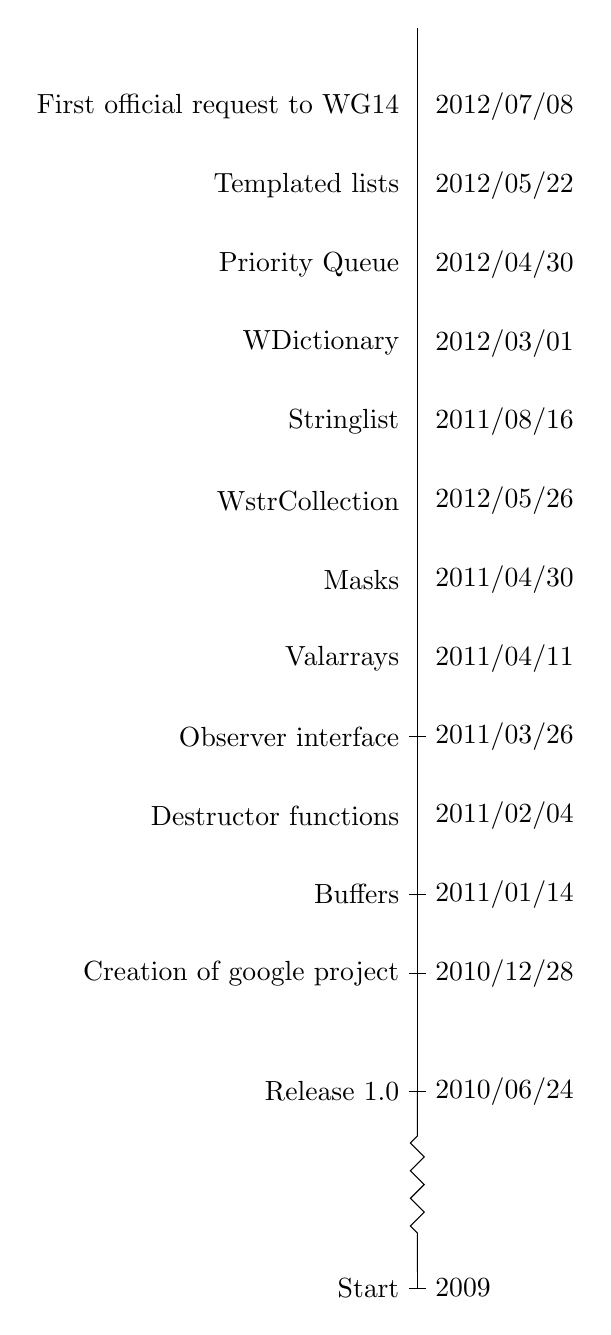
\begin{tikzpicture}[snake=zigzag, line before snake = 5mm, line after snake = 5mm]
%draw vertical line   
\draw (1,0) -- (1,0.2);
\draw[snake] (1,0.2) -- (1,2.5);
\draw (1,2.5) -- (1,16);

%draw vertical lines
\foreach \y in {0,2.5,4,5,7}
   \draw (1cm - 3pt, \y cm) -- (1cm + 3pt,\y cm);

%draw nodes
\draw (1,0) node[left=3pt] { Start } node[right=3pt] {2009};
\draw (1,2.5) node[left=3pt] { Release 1.0 } node[right=3pt] {2010/06/24};
\draw (1,4) node[left=3pt] { Creation of google project } node[right=3pt] {2010/12/28};
\draw (1,5) node[left=3pt] {Buffers} node[right=3pt] {2011/01/14};
\draw (1,6) node[left=3pt] {Destructor functions} node[right=3pt] {2011/02/04};
\draw (1,7) node[left=3pt] {Observer interface} node[right=3pt] {2011/03/26};
\draw (1,8) node[left=3pt] {Valarrays} node[right=3pt] {2011/04/11};
\draw (1,9) node[left=3pt] {Masks} node[right=3pt] {2011/04/30};

\draw (1,10) node[left=3pt] {WstrCollection} node[right=3pt] {2012/05/26};

\draw (1,11) node[left=3pt] {Stringlist} node[right=3pt] {2011/08/16};
\draw (1,12) node[left=3pt] {WDictionary} node[right=3pt] {2012/03/01};
\draw (1,13) node[left=3pt] {Priority Queue} node[right=3pt] {2012/04/30};
\draw (1,14) node[left=3pt] {Templated lists} node[right=3pt] {2012/05/22};
\draw (1,15) node[left=3pt] {First official request to WG14} node[right=3pt] {2012/07/08};
\end{tikzpicture}
\fi
\printindex
\iftth\else
% Author: Till Tantau
% Source: The PGF/TikZ manual
\pagestyle{empty}
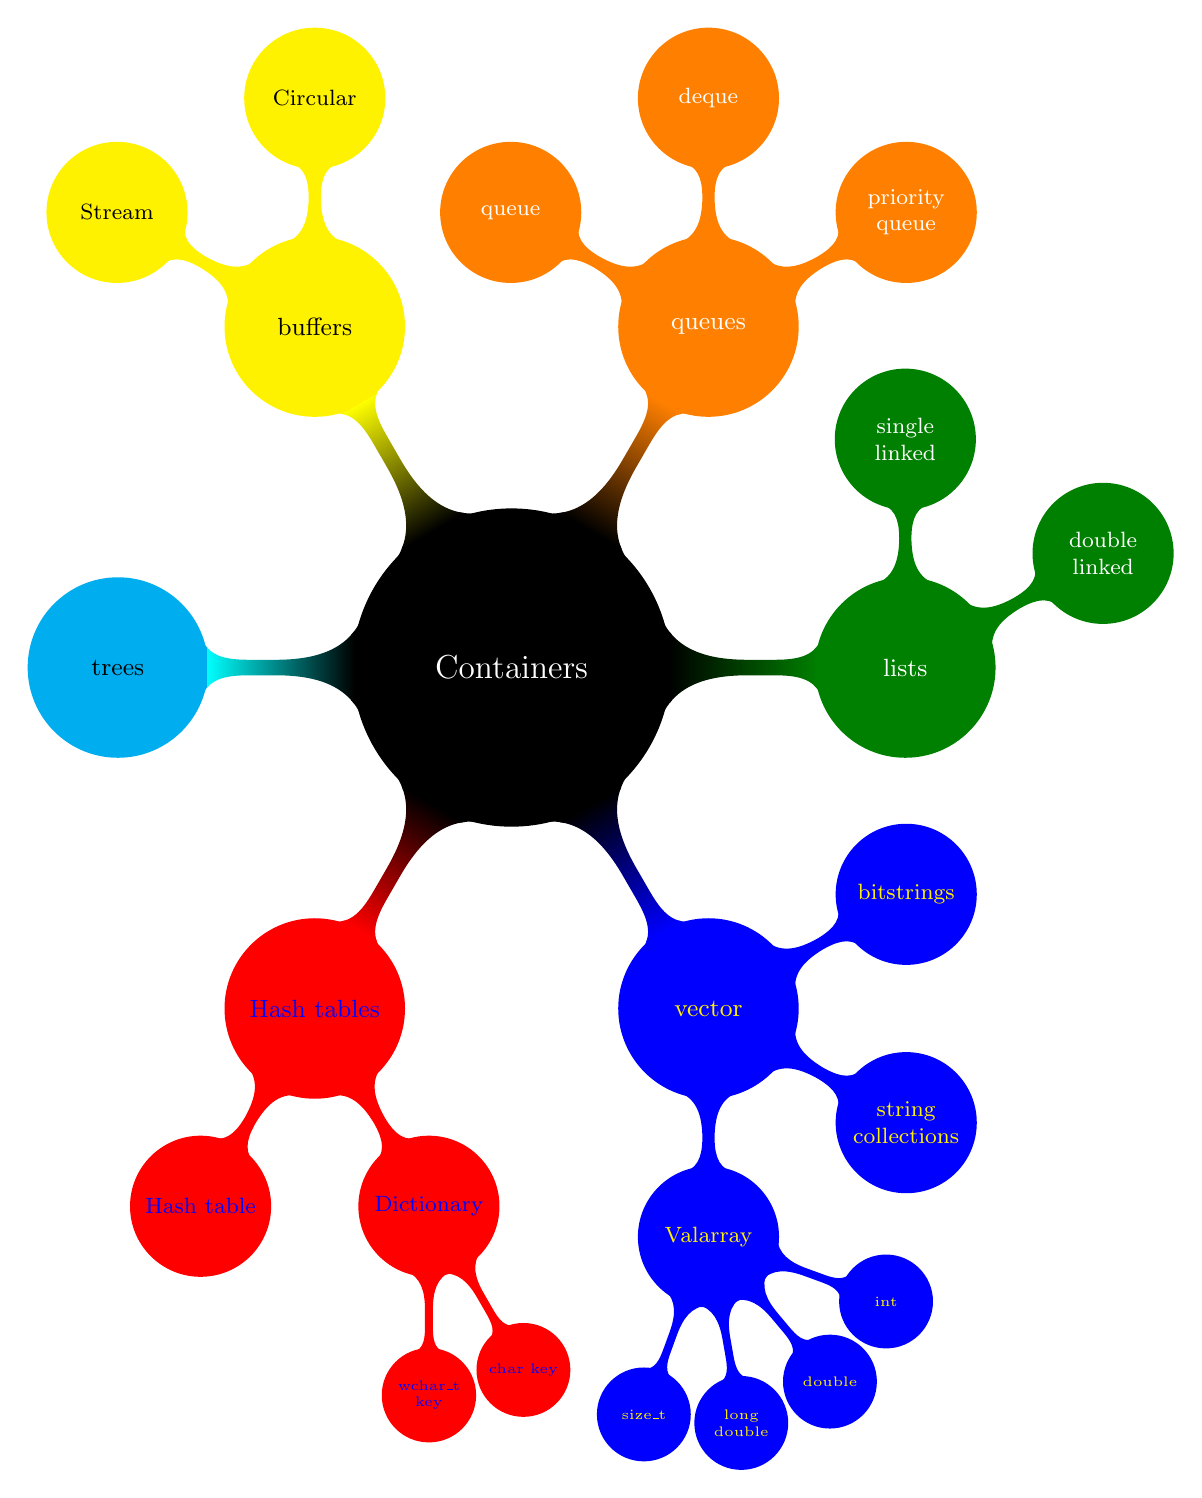
\begin{tikzpicture}
  \path[mindmap,concept color=black,text=white]
    node[concept] {Containers}
    [clockwise from=0]
    child[concept color=green!50!black] {
      node[concept] {lists}
      [clockwise from=90]
      child { node[concept] {single linked} }
      child { node[concept] {double linked} }
    }  
    child[concept color=lightblue,text=yellow] {
      node[concept] {vector}
      [clockwise from=30 ]
      child { node[concept] {bitstrings} }
      child { node[concept] {string collections} }
      child { node[concept ] {Valarray} 
          [clockwise from=-20]
          child { node[concept] {int} }
          child { node[concept] {double} }
          child { node[concept] {long double} }
          child { node[concept] {size\_t} }
      }
    }
    child[concept color=lightred,text=blue] { 
       node[concept] {Hash tables} 
      [clockwise from=-60]
      child { node[concept ] {Dictionary} 
          [clockwise from=-60]
           child { node[concept] {char key} }
           child { node[concept] {wchar\_t key} }
      }
      child { node[concept] {Hash table} }
    }
    child[concept color=cyan,text=black] { node[concept] {trees} }
    child[concept color=yellow,text=black] { node[concept] {buffers} 
      [clockwise from=150]
      child { node[concept] {Stream} }
      child { node[concept] {Circular} }
    }
    child[concept color=orange] { node[concept] {queues} 
      [clockwise from=150]
      child { node[concept] {queue} }
      child { node[concept] {deque} }
      child { node[concept] {priority queue} }
 };
\end{tikzpicture}
\fi
\end{document}
